\documentclass[a4paper, 12pt]{memoir}
\usepackage[utf8]{inputenc}
\usepackage[english]{babel}
\usepackage{concmath}
\usepackage{tgschola}
\usepackage[T1]{fontenc}
\usepackage{amssymb}
\usepackage{amsthm}
\usepackage{mathtools}
\usepackage{algorithm}
\usepackage[noend]{algpseudocode}
\usepackage{bm}
\usepackage{xcolor}
\usepackage{listings}
\usepackage{caption}
\usepackage{standalone}
\usepackage{fancyhdr}
\usepackage[fit, breakall]{truncate}
\usepackage{bookmark}
\usepackage{titlesec}
\usepackage[margin=1.3in]{geometry}


\usepackage{soul}
\definecolor{nicered}{rgb}{0,.5,.55} %{.647,.129,.149}
\makeatletter
\newlength\dlf@normtxtw
\setlength\dlf@normtxtw{\textwidth}
\def\myhelvetfont{\def\sfdefault{mdput}}
\newsavebox{\feline@chapter}
\newcommand\feline@chapter@marker[1][4cm]{%
\sbox\feline@chapter{%
\resizebox{!}{#1}{\fboxsep=1pt%
\colorbox{nicered}{\color{white}\bfseries\sffamily\thechapter}%
}}%
\rotatebox{90}{%
\resizebox{%
\heightof{\usebox{\feline@chapter}}+\depthof{\usebox{\feline@chapter}}}%
{!}{\scshape\so\@chapapp}}\quad%
\raisebox{\depthof{\usebox{\feline@chapter}}}{\usebox{\feline@chapter}}%
}
\newcommand\feline@chm[1][4cm]{%
\sbox\feline@chapter{\feline@chapter@marker[#1]}%
\makebox[0pt][l]{% aka \rlap
\makebox[1cm][r]{\usebox\feline@chapter}%
}}
\makechapterstyle{daleif1}{
\renewcommand\chapnamefont{\normalfont\Large\scshape\raggedleft\so}
\renewcommand\chaptitlefont{\normalfont\huge\bfseries\scshape\color{nicered}}
\renewcommand\chapternamenum{}
\renewcommand\printchaptername{}
\renewcommand\printchapternum{\null\hfill\feline@chm[2.5cm]\par}
\renewcommand\afterchapternum{\par\vskip\midchapskip}
\renewcommand\printchaptertitle[1]{\chaptitlefont\raggedleft ##1\par}
}
\makeatother
\chapterstyle{daleif1}


\definecolor{section}{rgb}{0,.5,.55}


%\newtheorem{theorem}{Theorem}
\newtheorem*{theorem*}{Theorem}
%\newtheorem{lemma}{Lemma}
\newtheorem*{lemma*}{Lemma}

\newtheoremstyle{style}
{0pt}
{12pt}
{\centering\itshape\color{black}}
{}
{\color{white}}
{}
{0em}
{\centering}

\theoremstyle{style}
\newtheorem{theorem}{Theorem}
\newtheorem{lemma}{Lemma}


\renewcommand\qedsymbol{$\blacksquare$}
\DeclareMathOperator*{\nullspace}{null}
\newcommand{\pluseq}{\mathrel{+}=}
\newcommand{\minuseq}{\mathrel{-}=}
\pdfstringdefDisableCommands{\let\bm=\relax}


\newcommand{\sep}{
    \begin{center}
        \vspace{1\baselineskip}
    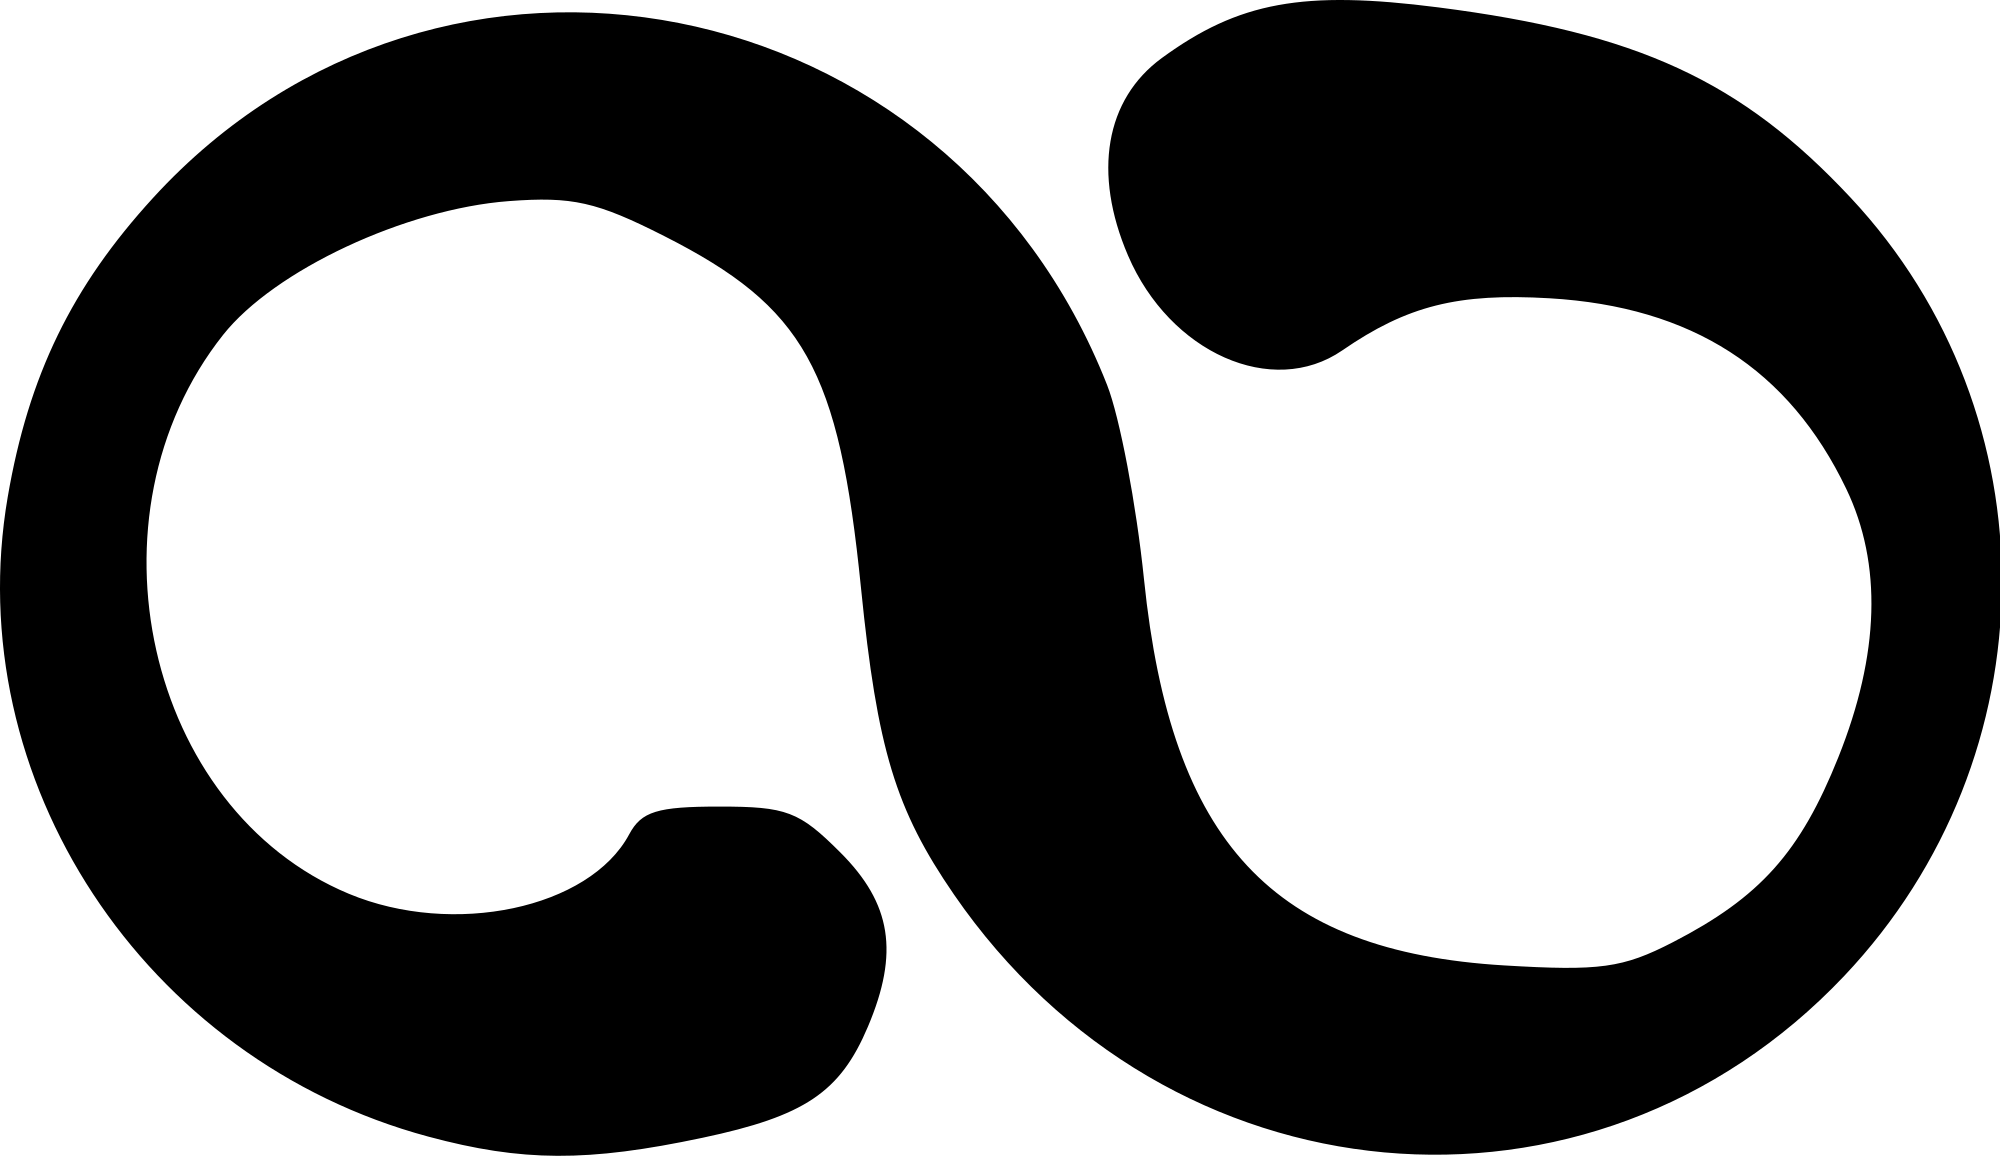
\includegraphics[width=0.75cm]{../resources/jpg/eulers_infinity.png}
\end{center}
}


\makeatletter
\newcommand\fs@nobottomruled{\def\@fs@cfont{\bfseries}\let\@fs@capt\floatc@ruled
  \def\@fs@pre{\hrule height.8pt depth0pt \kern2pt}%
  \def\@fs@post{}% Formerly \def\@fs@post{\kern2pt\hrule\relax}%
  \def\@fs@mid{\kern2pt\hrule\kern2pt}%
  \let\@fs@iftopcapt\iftrue}
\makeatother


\floatstyle{nobottomruled}
\restylefloat{algorithm}


\lstset{
    numbers=left,
    stepnumber=1,
    numbersep=5pt,
    numberstyle=\small\color{lightgray},
    basicstyle=\ttfamily\color{black},
    keywordstyle=\color{teal},
    commentstyle=\color{lightgray},
    stringstyle=\color{cyan},
    identifierstyle=\color{black},
    frame=none,
    rulecolor=\color{darkgray},
    tabsize=4,
    backgroundcolor=\color{white}
}


%\setsecnumdepth{subsection}


\hypersetup{
    pdftitle={Book of Proofs},
    pdfsubject={Discrete Mathematics},
    bookmarksnumbered=true,
    bookmarksopenlevel=1,
    bookmarksdepth=2,
    hidelinks,
    pdfstartview=Fit,
    pdfpagemode=UseOutlines,
    pdfpagelayout=TwoPageRight,
    }

\bookmarksetup{depth=2}
\setcounter{tocdepth}{2}


\fancyhf{}
\fancyhead[LE, RO]{\truncate{0.33 \textwidth} \rightmark}
\fancyhead[RE, LO]{ \leftmark}


%\definecolor{section}{rgb}{0,.5,.55}

\titlespacing*{\section}
    {0pt}{3.7ex plus 1ex minus .2ex}{4.3ex plus .2ex}
\titleformat{\section}{
    \normalfont\fontsize{18}{15}\bfseries\raggedright
    }{
        \textbf{Section }
        \color{section}
        \thesection\color{black}
        \hspace{0cm}
        \textbf{:}
    }{1em}{}

\titlespacing*{\subsection}
    {0pt}{3.7ex plus 1ex minus .2ex}{3.3ex plus .2ex}

% \setsecnumformat{\csname #1secnumformat\endcsname}
%     \newcommand\subsectionsecnumformat{
%         \raggedleft
%         \color{section}
%         \thesubsection
%         \hspace{0.5cm}
%     }


\begin{document}


\pagestyle{fancy}
\raggedbottom


\frontmatter
% =================================== Title ===================================
\documentclass[preview]{standalone}


%\makeatletter \newcommand\HUGE{\@setfontsize\Huge{38}{47}} \makeatother


\begin{document}
    \begin{titlingpage}
        \hypertarget{pdftitle}{}
        \bookmark[dest=pdftitle, level=chapter]{Title}
        \centering
        \hfill 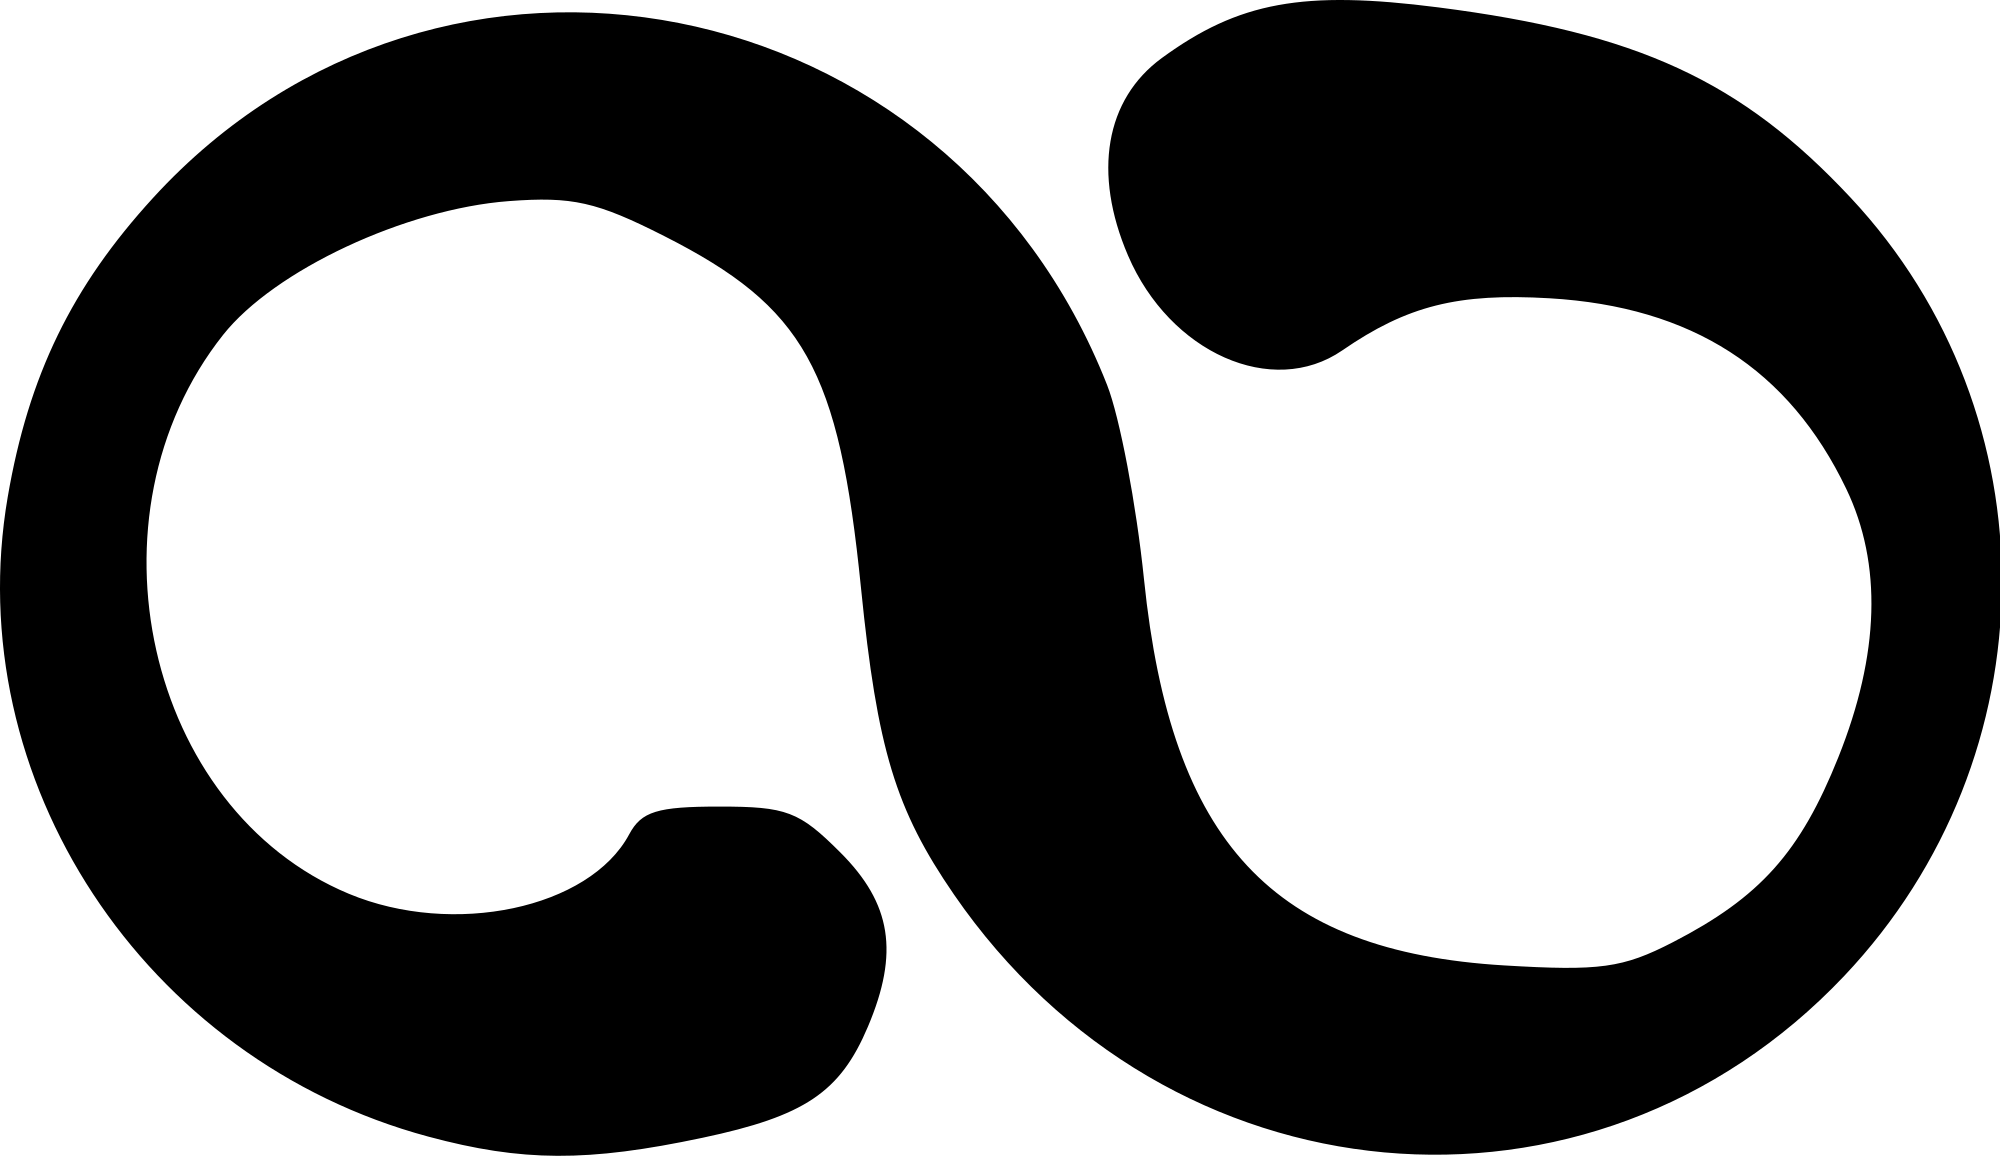
\includegraphics[width=2cm]{../resources/jpg/eulers_infinity.png} \par
        \vspace{4\baselineskip}
        \raggedleft \scshape \Large DISCRETE MATHEMATICS \par
        \vspace{2\baselineskip}
        \scalebox{2}{\fontsize{22pt}{0pt} \textbf{\scshape{Book of Proofs}}} \par
        \vspace{4\baselineskip}
        %\scshape \large Author: Chris Hamberg \par
        \scshape \large chris.hamberg@programmer.net \par      
    \end{titlingpage}
\end{document}


% ==================================== TOC ====================================
\cfoot{\thepage}
\tableofcontents


\mainmatter
\cfoot{\thepage}
% ================================= Chapter 1 =================================
\chapter{Introduction to Proofs}
\documentclass[preview]{standalone}


\begin{document}

\section{Theorems}
\begin{figure}[h!]
    \centering
    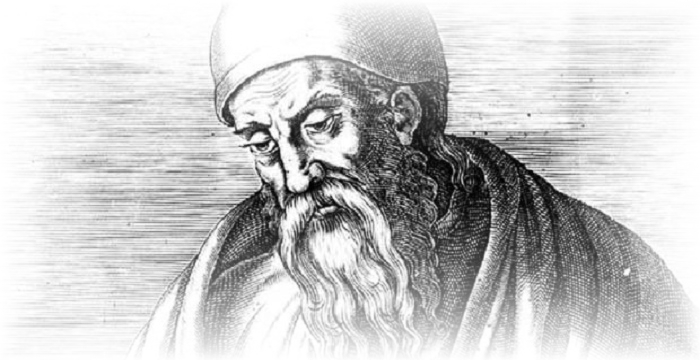
\includegraphics[width=9.5cm]{../resources/jpg/1.6.introduction.to.proofs/euclid.jpg}
    \caption*{\emph{Euclid.}}
\end{figure} 

% ============================== 0001 Theorem 1601 ================================
\subsection[The sum of two odd integers is even.]{\color{section} Theorem 1 \color{black} : the sum of two odd integers is even.}
\documentclass[preview]{standalone}
\usepackage{amssymb, amsthm}
\usepackage{mathtools}
\usepackage{bm}


\newtheorem{theorem}{Theorem}
\renewcommand\qedsymbol{$\blacksquare$}


\begin{document}
    
\begin{theorem} %[\textbf{1601}]
    Let \bm{$\chi$} and \bm{$\zeta$} be integers. 
    If \bm{$\chi$} and \bm{$\zeta$} are odd, 
    then \bm{$\chi + \zeta$} is even.
\end{theorem}

\begin{proof}
    By the definition for odd numbers, 
    there exists integers \bm{$\mu$} and \bm{$\nu$} such that 
    \bm{$\chi = 2\mu + 1$} and \bm{$\zeta = 2\nu + 1$}. 
    Hence,
    \begin{equation*}
        \chi + \zeta 
            = 
        \Big[
            \big \langle 2 \mu + 1 \big \rangle 
                + 
            \big \langle 2 \nu + 1 \big \rangle
        \Big]
            = 
        \Big[
            2 \big \langle \mu + \nu + 1 \big \rangle
        \Big]
    \end{equation*} 
    Integers are closed under addition. 
    Thus, the factor 
    \bm{$\big \langle \mu + \nu + 1 \big \rangle$} is an integer. 
    It follows that \bm{$\chi + \zeta$} is even, 
    by the definition for even numbers.
\end{proof}


\end{document}
\pagebreak


% ============================== 0002 Theorem 1602 =================================
\subsection[The sum of two even integers is even.]{\color{section} Theorem 2 \color{black} : the sum of two even integers is even.}
\documentclass[preview]{standalone}
\usepackage{amssymb, amsthm}
\usepackage{mathtools}
\usepackage{bm}


\newtheorem{theorem}{Theorem}
\renewcommand\qedsymbol{$\blacksquare$}


\begin{document}

\begin{theorem} %[\textbf{1602}]
    Let \bm{$\chi$} and \bm{$\zeta$} be integers. 
    If \bm{$\chi$} and \bm{$\zeta$} are even, 
    then \bm{$\chi + \zeta$} is even.
\end{theorem}

\begin{proof}
    By the definition for even numbers, 
    there exist integers \bm{$\mu$} and \bm{$\nu$} such that 
    \bm{$2\mu = \chi$} and \bm{$2\nu = \zeta$}. 
    Hence,
    \begin{equation*}
        \chi + \zeta 
            = 
        \Big[
            \big \langle 2\mu \big \rangle
                + 
            \big \langle 2\nu \big \rangle
        \Big]
            =
        \Big[ 
            2 \big \langle \mu + \nu \big \rangle
        \Big]
    \end{equation*} 
    Integers are closed under addition. 
    Thus, the factor 
    \bm{$\big \langle \mu + \nu \big \rangle$} 
    is an integer. 
    It follows that \bm{$\chi + \zeta$} is even, 
    by the definition for even numbers.
\end{proof}


\end{document}
\sep


% ============================== 0003 Theorem 1603 =================================
\subsection[The square of an even number is even.]{\color{section} Theorem 3 \color{black} : the square of an even number is even.}
\documentclass[preview]{standalone}
\usepackage{amssymb, amsthm}
\usepackage{mathtools}
\usepackage{bm}


\newtheorem{theorem}{Theorem}
\renewcommand\qedsymbol{$\blacksquare$}


\begin{document}
    
\begin{theorem} %[\textbf{1603}]
    If \bm{$\chi$} is an even integer, 
    then \bm{$\chi^2$} is an even integer.
\end{theorem}

\begin{proof}
    By the definition for even numbers, 
    there exists an integer \bm{$\eta$} such that 
    \bm{$\chi = 2\eta$}. 
    Hence,
    \begin{equation*}
        \big \langle 2 \eta \big \rangle ^2 
            = 
        4 \eta ^2 
            = 
        2 \big \langle 2 \eta ^2 \big \rangle
    \end{equation*}
    Integers are closed under multiplication. 
    Thus, the factor 
    \bm{$\big \langle 2 \eta ^2 \big \rangle$} is an integer. 
    It follows that \bm{$\chi^2$} is even, by 
    the definition for even numbers.
\end{proof}


\end{document}
\sep


% ============================== 0004 Theorem 1604 =================================
\subsection[The additive inverse of an even number.]{\color{section} Theorem 4 \color{black} : the additive inverse of an even number.}
\documentclass[preview]{standalone}
\usepackage{amssymb, amsmath, amsthm}
\usepackage{mathtools}
\usepackage{bm}


\newtheorem{theorem}{Theorem}
\renewcommand\qedsymbol{$\blacksquare$}


\begin{document}


\begin{theorem} %[\textbf{1604}]
    The additive inverse of an even number is an even number.
\end{theorem}

\begin{proof}
    Let \bm{$\chi$} be an even number. 
    There exists an integer \bm{$\eta$} such that 
    \bm{$\chi = 2\eta$}, 
    by the definition for even numbers. 
    The additive inverse for \bm{$\chi$} is,
    \begin{equation*}
        -1 \big \langle \chi \big \rangle
            = 
        -1 \big \langle 2 \eta \big \rangle
    \end{equation*} 
    By commutativity of multiplication that is,
    \begin{equation*}
        -1 \big \langle 2 \eta \big \rangle
            = 
        2 \big \langle - \eta \big \rangle
    \end{equation*}
    Since integers are closed under multiplication, 
    the factor \bm{$\big \langle - \eta \big \rangle$} is an integer. 
    It follows that the additive inverse of \bm{$\chi$} is an even number, 
    by the definition for even numbers.
\end{proof}


\end{document} 
\pagebreak


% ============================== 0005 Theorem 1605 =================================
\subsection[A special parity.]{\color{section} Theorem 5 \color{black} : a special parity.}
\documentclass[preview]{standalone}
\usepackage{amssymb, amsthm}
\usepackage{mathtools}
\usepackage{bm}


\newtheorem{theorem}{Theorem}
\renewcommand\qedsymbol{$\blacksquare$}


\begin{document}


\begin{theorem} %[\textbf{1605}]
    Let \bm{$\mu$}, \bm{$\zeta$}, and \bm{$\pi$} be integers. 
    If \bm{$\mu + \zeta$} and \bm{$\zeta + \pi$} are even, 
    then \bm{$\mu + \pi$} is even.
\end{theorem}

\begin{proof}
    By the hypothesis, 
    there exist integers \bm{$\sigma$} and \bm{$\epsilon$} such that 
    \bm{$\mu + \zeta = 2\sigma$}, 
    and \bm{$\zeta + \pi = 2\epsilon$}. 
    Hence, 
    \begin{equation*}
        \big \langle \mu + \zeta \big \rangle 
            + 
        \big \langle \zeta + \pi \big \rangle
            = 
        2 \sigma + 2 \epsilon
    \end{equation*}
    Subtracting \bm{$2\zeta$} from both sides, 
    by the subtraction property of equality for equations, 
    produces
    \begin{equation*}
        \Big \langle \mu + \pi \Big \rangle
            = 
        \Big \langle 2 \sigma + 2 \epsilon - 2 \zeta \Big \rangle
            = 
        \Big[ 2 \big \langle \sigma + \epsilon - \zeta \big \rangle \Big]
    \end{equation*}
    \bm{$\sigma$} and \bm{$\epsilon$} are integers,
    by the definition for even numbers, 
    and \bm{$\zeta$} is an integer by the hypothesis. 
    Since addition and subtraction are closed on integers, 
    the factor 
    \bm{$\big \langle \sigma + \epsilon - \zeta \big \rangle$} 
    is an integer. 
    It follows that \bm{$\mu + \pi$} is an even, 
    by the definition for 
    even numbers.
\end{proof}


\end{document}
\begin{center}
    
\includegraphics[width=6cm]{../resources/jpg/1.6.introduction.to.proofs/olympics.jpg}
\end{center}


% ============================== 0006 Theorem 1606 =================================
\subsection[The product of two odd numbers is odd.]{\color{section} Theorem 6 \color{black} : the product of two odd numbers is odd.}
\documentclass[preview]{standalone}
\usepackage{amssymb, amsthm}
\usepackage{mathtools}
\usepackage{bm}


\newtheorem{theorem}{Theorem}
\renewcommand\qedsymbol{$\blacksquare$}


\begin{document}


\begin{theorem} %[\textbf{1606}]
    The product of two odd numbers is odd.
\end{theorem}

\begin{proof}
    Suppose that \bm{$\mu$} and \bm{$\zeta$} are odd numbers. 
    By the definition for odd numbers, 
    there exist integers \bm{$\sigma$} and \bm{$\epsilon$} such that 
    \bm{$\mu = 2\sigma + 1$} and \bm{$\zeta = 2\epsilon + 1$}. 
    Thus, the product of odd numbers \bm{$\mu \zeta$} is,
    \begin{equation*}
        \mu \zeta 
            =
        \Big[ 
            \big \langle 2 \sigma + 1 \big \rangle 
            \big \langle 2 \epsilon + 1 \big \rangle
        \Big]
            = 
        \Big[% \langle
            2 \sigma 2 \epsilon + 2 \sigma + 2 \epsilon + 1 
        \Big]% \rangle
            = 
        \Big[
            2 \big \langle 
                \sigma \epsilon + \sigma + \epsilon 
            \big \rangle 
                + 1
        \Big]
    \end{equation*}     
    The factor 
    \bm{$\big \langle \sigma \epsilon + \sigma + \epsilon \big \rangle$} 
    is an integer because \bm{$\sigma$} and \bm{$\epsilon$} are integers by definition, 
    and integers are closed on addition. 
    Therefore, \bm{$\mu \zeta$} is odd by the definition for odd numbers.
\end{proof}


\end{document}
\pagebreak


% ============================== 0007 Theorem 1608 =================================
\subsection[Two plus a perfect square is not perfect.]{\color{section} Theorem 7 \color{black} : two plus a perfect square is not perfect.}
\documentclass[preview]{standalone}
\usepackage{amssymb, amsthm}
\usepackage{mathtools}
\usepackage{bm}


\newtheorem{theorem}{Theorem}
\renewcommand\qedsymbol{$\blacksquare$}


\begin{document}


\begin{theorem} %[\textbf{1608}]
    If \bm{$\eta$} is a perfect square, 
    then \bm{$\eta + 2$} is not a perfect square.
\end{theorem}

\begin{proof}
    Let \bm{$\eta$} be a perfect square. 
    Assume \bm{$\eta + 2$} is a perfect square for the purpose of contradiction. 
    By the definition of perfect square, 
    \bm{$\sqrt{\eta}$} has to be an integer, 
    and by our assumption there exists an integer \bm{$\zeta$} such that 
    \bm{$\zeta^2 = \eta + 2$}. 
    So the equivalence 
    \bm{$\zeta^2 - \big \langle \sqrt{\eta} \big \rangle ^2 = 2$} 
    must be the difference of squares 
    %\begin{equation*}
    \bm{$
        \big \langle \zeta + \sqrt{\eta} \big \rangle 
        \big \langle \zeta - \sqrt{\eta} \big \rangle 
            =
        2
    $}.
    %\end{equation*}
    Since integers are closed on addition and subtraction, 
    it follows that the factors of \bm{$2$}, 
    \bm{$\big \langle \zeta + \sqrt{\eta} \big \rangle$} and 
    \bm{$\big \langle \zeta - \sqrt{\eta} \big \rangle$}, 
    have to be integers. 
    Because \bm{$2$} is prime, those integer factors can only be elements in the set
    \bm{$\{-2, -1, 1, 2\}$}. Thus, there are exactly two possibilities:
    \\ \\ \indent \indent \bm{$(i)$} $\zeta ^2 - \big \langle \sqrt{\eta} \big \rangle ^2 = 
                            \big \langle 2 \big \rangle \big \langle 1 \big \rangle$,
    \\ \indent \indent or \bm{$(ii)$} $\zeta ^2 - \big \langle \sqrt{\eta} \big \rangle ^2 =
                            \big \langle -1 \big \rangle \big \langle -2 \big \rangle.$
    \\ \\ In case \bm{$(i)$}, without loss of generality, 
    we have a system of linear equations in two variables \bm{$\zeta$} and \bm{$\sqrt{\eta}$}:
    \begin{equation*}
        \zeta + \sqrt{\eta} = 2
    \end{equation*}
    \begin{equation*}
        \zeta - \sqrt{\eta} = 1
    \end{equation*}
    The matrix of coefficients 
    $\bm{\Psi = } \left[\begin{smallmatrix}
        \bm{1} & \bm{1} \\
        \bm{1} & \bm{-1} 
    \end{smallmatrix}\right]$, 
    the inverse for which is
    $\bm{\Psi^{-1} = } \left[\begin{smallmatrix}
        \bm{0.5} & \bm{0.5} \\
        \bm{0.5} & \bm{-0.5}
    \end{smallmatrix}\right]$. 
    The product of \bm{$\Psi^{-1}$} and the matrix of solutions yields \bm{$\zeta = 1.5$}, 
    which is not in \bm{$\mathbb{Z}$}; 
    contradicting the assumption that \bm{$\zeta^2$} was a perfect square.
    \\ \\ 
    In case \bm{$(ii)$}, 
    we are presented with a similar system of linear equations. 
    The only difference in this system compared to \bm{$(i)$} is the matrix of solutions 
    $\bm{\Phi = } \left[\begin{smallmatrix}
        \bm{-1} \\
        \bm{-2}
    \end{smallmatrix}\right]$. 
    \bm{$\Psi^{-1}\Phi$} yields \bm{$\zeta = -1.5$}, 
    which is not in \bm{$\mathbb{Z}$}, 
    a contradiction. 
    Thus, the assumption that \bm{$\zeta^2$} was a perfect square must be false in this case, as well.
    \\ \\
    Since the assumption proves false in all possible cases, 
    it is not possbile that both \bm{$\eta + 2$}, and \bm{$\eta$} are perfect squares.
\end{proof}


\end{document}
\vspace{1\baselineskip}
\begin{figure}[h!]
    \centering
    
\includegraphics[width=2cm]{../resources/jpg/1.6.introduction.to.proofs/zeus.jpg}
\end{figure} 
\pagebreak


% ============================== 0008 Theorem 1609 =================================
\subsection[A sum of irrational and rational numbers.]{\color{section} Theorem 8 \color{black} : a sum of irrational and rational numbers.}
\documentclass[preview]{standalone}
\usepackage{amssymb, amsthm}
\usepackage{mathtools}
\usepackage{bm}


\newtheorem{theorem}{Theorem}
\renewcommand\qedsymbol{$\blacksquare$}


\begin{document}


\begin{theorem} %[\textbf{1609}]
    The sum of an irrational number and a rational number is irrational.
\end{theorem}

\begin{proof}
    By contradiction. Suppose that \bm{$\mu$} and \bm{$\zeta$} are rational numbers, 
    and let \bm{$\chi$} be an irrational number. 
    For the purpose of contradiction, 
    assume the negation of the hypothesis. 
    That is, the proposition 
        $$\lnot p: \emph{the sum of an irrational number and a rational number 
        is rational.}$$
    Hence, \bm{$\chi \textbf{ + } \mu \textbf{ = } \zeta$}, 
    by the assumption \bm{$\lnot p$}. 
    Thus, 
    \bm{$\chi \textbf{ = } \zeta \textbf{ + } \big \langle \textbf{ - } \mu \big \rangle$}, 
    by the additive equality property for equations. 
    But rational numbers are closed under addition by the closure property for rational numbers. 
    So \bm{$\lnot p$} implies \bm{$\chi$} is rational, 
    and \bm{$\chi$} is irrational; a contradiction.
\end{proof}


\end{document}
\begin{figure}[h!]
    \centering
    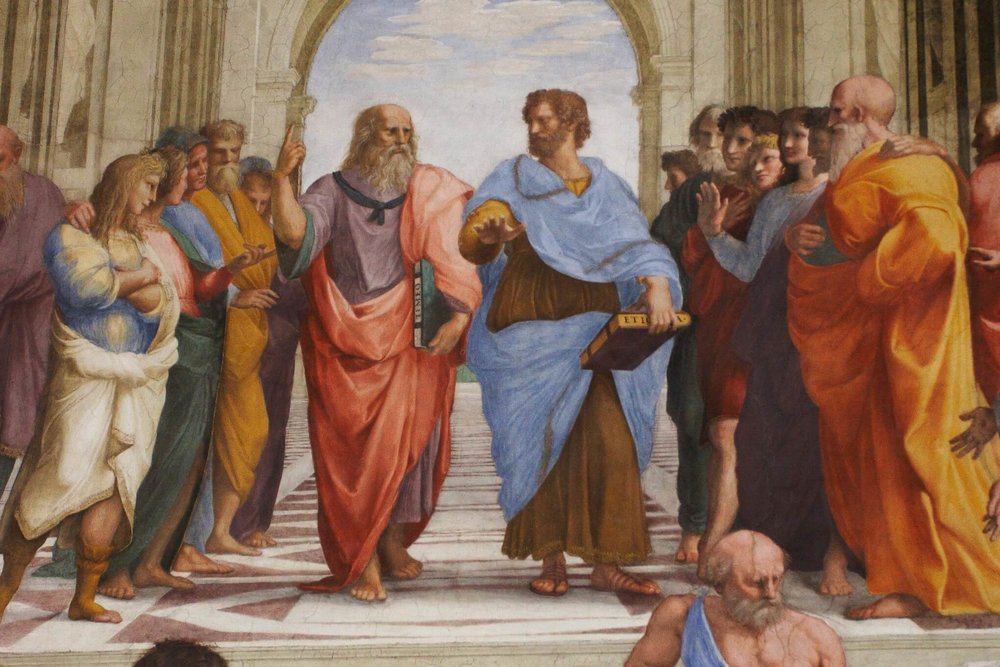
\includegraphics[width=12.5cm]{../resources/jpg/1.6.introduction.to.proofs/plato-republic.jpg}
    \caption*{\emph{Plato and Aristotle.}}
\end{figure}


% ============================== 0009 Theorem 1610 ================================
\subsection[The product of two rational numbers.]{\color{section} Theorem 9 \color{black} : the product of two rational numbers.}
\documentclass[preview]{standalone}
\usepackage{amssymb, amsthm}
\usepackage{mathtools}
\usepackage{bm}


\newtheorem{theorem}{Theorem}
\renewcommand\qedsymbol{$\blacksquare$}


\begin{document}


\begin{theorem} %[\textbf{1610}]
    The product of two rational numbers is rational.
\end{theorem}

\begin{proof}
    Let \bm{$\mu$} and \bm{$\zeta$} be rational numbers. 
    By the definition for rational numbers, 
    there exist integers \bm{$\alpha$}, \bm{$\beta$}, \bm{$\gamma$}, and \bm{$\delta$} such that 
    \bm{$\mu = \frac{\alpha}{\beta}$} and \bm{$\zeta = \frac{\gamma}{\delta}$}. 
    The product of \bm{$\mu$} and \bm{$\zeta$} is \bm{$\frac{\alpha\gamma}{\beta\delta}$}. 
    Since integers are closed under multiplcation, 
    \bm{$\alpha\gamma$} and \bm{$\beta\delta$} are integers. 
    Thus \bm{$\mu\zeta$} is rational by definition.
\end{proof}


\end{document}
\pagebreak


% ============================== 0010 Theorem 1612 ================================
\subsection[An irrational times a rational number.]{\color{section} Theorem 10 \color{black} : an irrational times a rational number.}
\documentclass[preview]{standalone}
\usepackage{amssymb, amsthm}
\usepackage{mathtools}
\usepackage{bm}


\newtheorem{theorem}{Theorem}
\renewcommand\qedsymbol{$\blacksquare$}


\begin{document}


\begin{theorem} %[\textbf{1612}]
    The product of a nonzero rational number and an irrational number is 
    irrational.
\end{theorem}

\begin{proof}
    For the purpose of contradiction, assume the negation of the hypothesis; 
    the proposition 
        $$\lnot p : \emph{ the product of a nonzero rational number and an 
        irrational number}$$
        $\indent \indent \emph{is rational}$
        \\ \\
    Let \bm{$\alpha$}, \bm{$\beta$}, \bm{$\gamma$}, and \bm{$\delta$} be integers such that 
    \bm{$\alpha \neq 0$}, and let \bm{$\chi$} be an irrational number. 
    Then the proposition \bm{$\lnot p$} states 
    \begin{equation*}
        \Bigg(
            \frac{\alpha}{\beta} \space \cdot \space \chi 
        \Bigg)
            = 
        \Bigg(
            \frac{\gamma}{\delta}
        \Bigg)
    \end{equation*}    
    By the multiplicative equality property for equations, that is
    \begin{equation*}
        \Bigg(
            \chi
        \Bigg) 
            = 
        \Bigg(
            \frac{\gamma}{\delta} \space \cdot \space \frac{\beta}{\alpha} 
        \Bigg)
            =
        \Bigg( 
            \frac{\gamma\beta}{\delta\alpha}
        \Bigg)
    \end{equation*}
    By Theorem 9 (the closure property for multplication on rational numbers,) 
    \bm{$\chi$} is rational. 
    Thus, \bm{$\lnot p$} implies \bm{$\chi$} is rational and irrational.
\end{proof}


\end{document}
\sep


% ============================== 0011 Theorem 1613 ================================
\subsection[An irrational multiplicative inverse.]{\color{section} Theorem 11 \color{black} : an irrational multiplicative inverse.}
\documentclass[preview]{standalone}
\usepackage{amssymb, amsthm}
\usepackage{mathtools}
\usepackage{bm}


\newtheorem{theorem}{Theorem}
\renewcommand\qedsymbol{$\blacksquare$}


\begin{document}


\begin{theorem} %[\textbf{1613}]
    If \bm{$\chi$} is an irrational number, 
    then \bm{$\frac{1}{\chi}$} is irrational.
\end{theorem}

\begin{proof}
    By the contrapositive. 
    Suppose that \bm{$\frac{1}{\chi}$} is a rational number. 
    By the definition for rational numbers, 
    there exist integers \bm{$\alpha$} and \bm{$\gamma$} such that 
    \bm{$\frac{1}{\chi} = \frac{\alpha}{\gamma}$}. 
    Note that \bm{$\alpha$} is nonzero (because \bm{$\frac{1}{\chi}$} is nonzero.) 
    By the multiplicative property of equality for equations,
    \begin{equation*}
        \Bigg\{
            \left(
                \chi \cdot \frac{1}{\chi}
            \right) 
                = 
            \left(
                \chi \cdot \frac{\alpha}{\gamma}
            \right)
        \Bigg\} 
            \equiv
        \Bigg\{
            \left(
                \frac{\chi}{\chi} \cdot \frac{\gamma}{\alpha}
            \right) 
                = 
            \left(
                \frac{\chi \alpha}{\gamma} \cdot \frac{\gamma}{\alpha}
            \right)
        \Bigg\} 
            \equiv
        \Bigg\{
            \frac{\gamma}{\alpha} 
                = 
            \chi
        \Bigg\}
    \end{equation*}
    \bm{$\frac{\gamma}{\alpha} = \chi$} is rational, 
    by definition. 
    Thus, if \bm{$\frac{1}{\chi}$} is rational, 
    then \bm{$\chi$} is rational.
\end{proof}


\end{document}
\pagebreak


% ============================== 0012 Theorem 1614 ================================
\subsection[A rational multiplicative inverse.]{\color{section} Theorem 12 \color{black} : a rational multiplicative inverse.}
\documentclass[preview]{standalone}
\usepackage{amssymb, amsthm}
\usepackage{mathtools}
\usepackage{bm}


\newtheorem{theorem}{Theorem}
\renewcommand\qedsymbol{$\blacksquare$}


\begin{document}


\begin{theorem} %[\textbf{1614}]
    If \bm{$\chi$} is a rational number and 
    \bm{$\chi \neq 0$}, 
    then \bm{$\frac{1}{\chi}$} is rational.
\end{theorem}

\begin{proof}
    Let \bm{$\alpha$} and \bm{$\gamma$} be nonzero integers. 
    \bm{$\chi = \frac{\alpha}{\gamma}$}, 
    by the definition for rational numbers. 
    By the multiplicative property of equality for equations
    \begin{equation*}
        \left\{
            \left(
                \frac{1}{\chi} \cdot \chi
            \right) 
                = 
            \left(
                \frac{1}{\chi} \cdot \frac{\alpha}{\gamma}
            \right)
        \right\} 
            \equiv 
        \left\{
            \left(
                \frac{\chi}{\chi} \cdot \frac{\gamma}{\alpha}
            \right) 
                = 
            \left(
                \frac{\alpha}{\chi\gamma} \cdot \frac{\gamma}{\alpha}
            \right)
        \right\}
            \equiv 
        \left\{
            \frac{\gamma}{\alpha} 
                = 
            \frac{1}{\chi}
        \right\}
    \end{equation*}
    \bm{$\frac{\gamma}{\alpha} = \frac{1}{\chi}$} is rational, by definition. 
    Thus, if \bm{$\chi$} is a rational number and \bm{$\chi \neq 0$}, 
    then \bm{$\frac{1}{\chi}$} is rational.
\end{proof}


\end{document}
\begin{figure}[h!]
    \centering
    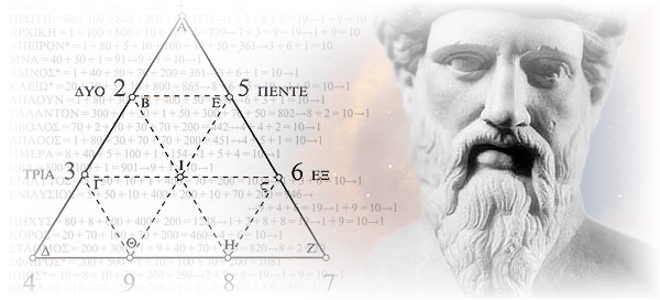
\includegraphics[width=13cm]{../resources/jpg/1.6.introduction.to.proofs/pythagoras.jpg}
    \caption*{\emph{Pythagoras.}}
\end{figure}


% ============================== 0013 Theorem 1615 ================================
\subsection[A corollary from additive compatibility.]{\color{section} Theorem 13 \color{black} : a corollary from additive compatibility.}
\documentclass[preview]{standalone}
\usepackage{amssymb, amsthm}
\usepackage{mathtools}
\usepackage{bm}


\newtheorem{theorem}{Theorem}
\renewcommand\qedsymbol{$\blacksquare$}


\begin{document}


\begin{theorem} %[\textbf{1615}]
    Let \bm{$\chi$} and \bm{$\zeta$} be real numbers. 
    If \bm{$\chi + \zeta \ge 2$}, 
    then 
    \bm{$
        \big \langle \chi \ge 1 \big \rangle 
            \lor
    $}
    \\
    \bm{$
        \big \langle \zeta \ge 1 \big \rangle
    $}.
\end{theorem}

\begin{proof}
    By the contrapositive.
    Suppose the negation of the consequent: 
    \begin{equation*}
        \big \langle \chi < 1 \big \rangle 
            \land 
        \big \langle \zeta < 1 \big \rangle    
    \end{equation*}    
    By additive compatibility,
    \begin{equation*}
        \Big \langle \chi + \zeta \Big \rangle 
            < 
        \Big \langle 1 + 1 \Big \rangle 
            = 
        \Big \langle 
            2
        \Big \rangle
    \end{equation*}
    This is the logical negation of the direct hypothesis. Thus concludes the proof.
\end{proof}


\end{document}
\pagebreak


% ============================== 0014 Theorem 1616 ================================
\subsection[Divisors of an even number.]{\color{section} Theorem 14 \color{black} : divisors of an even number.}
\documentclass[preview]{standalone}
\usepackage{amssymb, amsthm}
\usepackage{mathtools}
\usepackage{bm}


\newtheorem{theorem}{Theorem}
\renewcommand\qedsymbol{$\blacksquare$}


\begin{document}


\begin{theorem} %[\textbf{1616}]
    Let \bm{$\mu$} and \bm{$\zeta$} be integers. 
    If the product \bm{$\mu\zeta$} is even, 
    then \bm{$\mu$} is even or \bm{$\zeta$} is even.
\end{theorem}

\begin{proof}
    For the purpose of contraposition, suppose the negation of the consequent 
    \bm{$q$}
        $$\lnot q : \mu \text{\emph{ is odd and }} \zeta \text{\emph{ is odd.}}$$ 
    By definition, 
    there exist integers \bm{$\sigma$} and \bm{$\epsilon$} such that 
    \bm{$\mu = 2\sigma + 1$} and \bm{$\zeta = 2\epsilon + 1$}. 
    Thus, 
    \begin{equation*}
        \mu\zeta 
            =
        \Big[ 
            \big \langle 2 \sigma + 1 \big \rangle
            \big \langle 2 \epsilon + 1 \big \rangle 
        \Big]
            =
        \Big[ 
            2 
            \big \langle \sigma\epsilon + \sigma + \epsilon \big \rangle 
                + 
            1
        \Big]
    \end{equation*}
    The factor 
    \bm{$\big \langle \sigma \epsilon + \sigma + \epsilon \big \rangle$} 
    is an integer, 
    because integers are closed under addition and multiplication. 
    Thus, the product \bm{$\mu \zeta$} is odd, by definition.
\end{proof}


\end{document}
%\sep
\begin{figure}[h!]
    \centering
    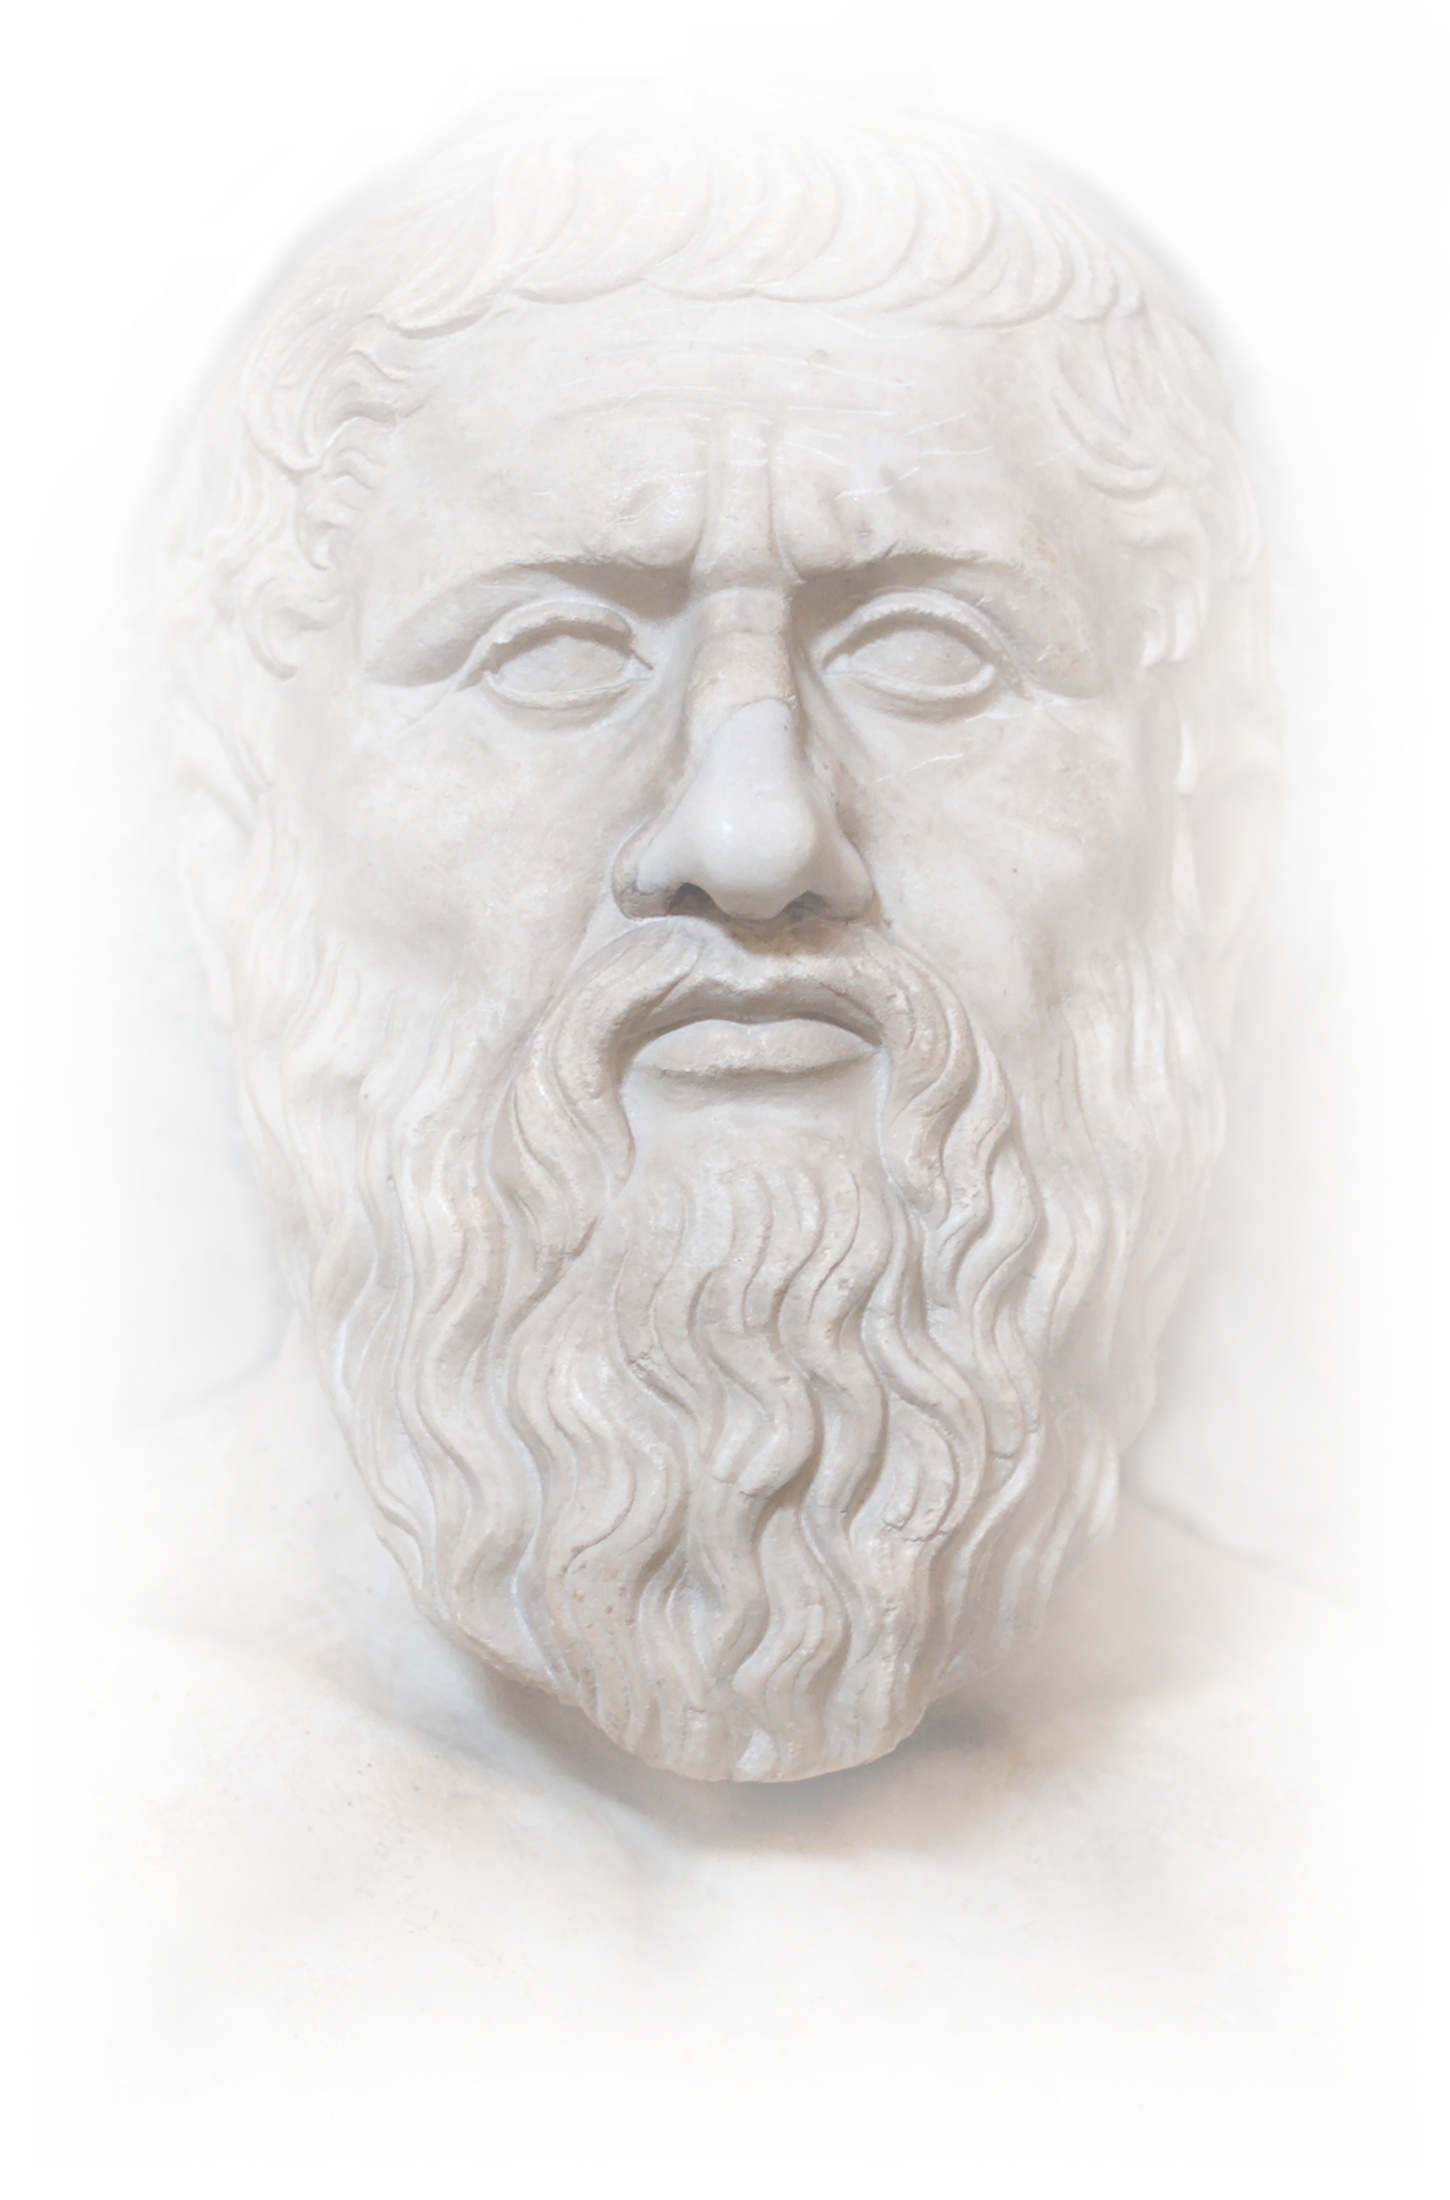
\includegraphics[width=8.5cm]{../resources/jpg/1.6.introduction.to.proofs/plato.jpg}
    \caption*{\emph{Plato.}}
\end{figure}
\pagebreak


% ============================== 0015 Theorem 1617 ================================
\subsection[\texorpdfstring{Odd integers of the form $\zeta ^3 + 5$.}
    {Odd integers of the form zeta cubed + 5.}
    ]{
        \color{section} Theorem 15 \color{black} : odd integers of the form \bm{$\zeta ^3 + 5$}.
    }
\documentclass[preview]{standalone}
\usepackage{amssymb, amsthm}
\usepackage{mathtools}
\usepackage{bm}


\newtheorem{theorem}{Theorem}
\renewcommand\qedsymbol{$\blacksquare$}


\begin{document}


\begin{theorem} %[\textbf{1617}]
    Let \bm{$\zeta$} be an integer. 
    If \bm{$\zeta^3 + 5$} is odd, 
    then \bm{$\zeta$} is even.
\end{theorem}

\begin{proof}
    By the contrapositive. 
    Suppose that \bm{$\zeta$} were odd. 
    By the definition for odd numbers, 
    there exists an integer \bm{$\gamma$} such that 
    \bm{$\zeta = 2 \gamma + 1$}. 
    By the Binomial Theorem,
    \begin{equation*}
        \Bigg \{
            \big \langle 2 \gamma + 1 \big \rangle ^3 + 5
        \Bigg \}
            = 
        \Bigg \{
            5 
                + 
            \sum\limits_{\iota=0} ^3 {3 \choose \iota} 
                2 \gamma ^{\langle 3 - \iota \rangle}
        \Bigg \}
            = 
        \Bigg \{
            2 
            \big \langle 4 \gamma ^3 - 6 \gamma ^2 + 3 \gamma + 3 \big \rangle
        \Bigg \}
    \end{equation*}
    The factor 
    \bm{$\big \langle 4 \gamma ^3 - 6 \gamma ^2 + 3 \gamma + 3 \big \rangle$} 
    is an integer because integers are closed on addition and multiplication. 
    Thus, \bm{$\zeta^3 + 5$} is even, by definition.
\end{proof}


\end{document}
\begin{figure}[h!]
    \centering
    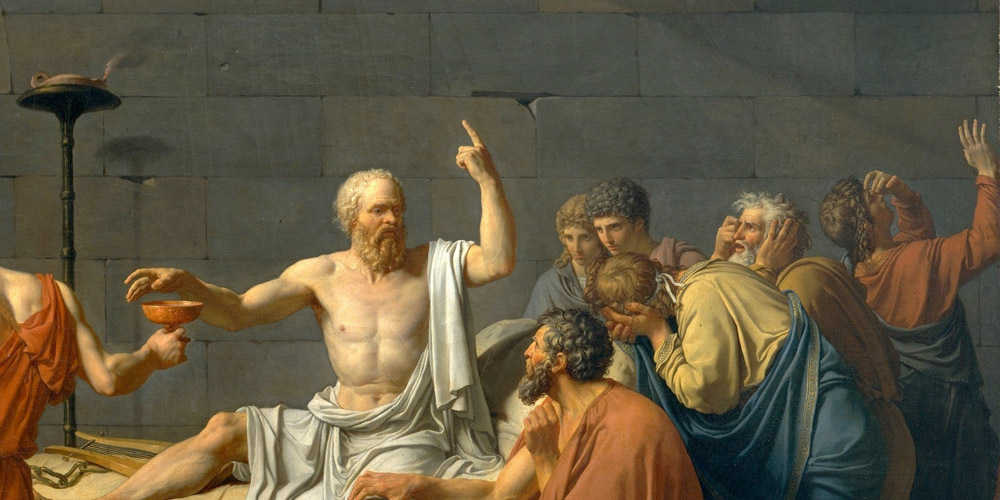
\includegraphics[width=13.25cm]{../resources/jpg/1.6.introduction.to.proofs/socrates.jpg}
    \caption*{\emph{Socrates with hemlock.}}
\end{figure}


% ============================== 0016 Theorem 1618 ================================
\subsection[\texorpdfstring{Even numbers of the form $3 \gamma + 2$}
        {Even numbers of the form $3 gamma + 2$}
    ]{
        \color{section} Theorem 16 \color{black} : even numbers of the form \bm{$3 \gamma + 2$}.
    }
\documentclass[preview]{standalone}
\usepackage{amssymb, amsthm}
\usepackage{mathtools}
\usepackage{bm}


\newtheorem{theorem}{Theorem}
\renewcommand\qedsymbol{$\blacksquare$}


\begin{document}


\begin{theorem} %[\textbf{1618}]
    Let \bm{$\gamma$} be an integer. 
    If \bm{$3 \gamma + 2$} is even, 
    then \bm{$\gamma$} is even.
\end{theorem}

\begin{proof}
    By the contrapositive. 
    Suppose \bm{$\gamma$} were odd. 
    By the definition of odd numbers,
    there exist an integer \bm{$\mu$} such that 
    \bm{$\gamma = 2 \mu + 1$}. 
    Thus,
    \begin{equation*}
        \Big \langle
            3 \big[ 2 \mu + 1 \big] + 2 
        \Big \rangle
            = 
        \Big \langle
            6 \mu + 5
        \Big \rangle
            =
        \Big \langle
            6 \mu + 4 + 1 
        \Big \rangle
            =
        \Big \langle
            2 \big[ 3 \mu + 2 \big] + 1
        \Big \rangle
    \end{equation*} 
    The factor \bm{$\big[ 3 \mu + 2 \big]$} is an integer, 
    since integers are closed on addition and multiplcation. 
    Thus, \bm{$3\gamma + 2$} is odd, by definition.
\end{proof}


\end{document}
\pagebreak


% ============================== 0017 Theorem 1625 ================================
\subsection[\texorpdfstring{$\rho$ does not exist.}
        {Rho does not exist.}
    ]{
        \color{section} Theorem 17 \color{black} : $\bm{\rho}$ does not exist.
    }
\documentclass[preview]{standalone}
\usepackage{amssymb, amsthm}
\usepackage{mathtools}
\usepackage{bm}


\newtheorem{theorem}{Theorem}
\renewcommand\qedsymbol{$\blacksquare$}


\begin{document}


\begin{theorem} %[\textbf{1625}]
    There does not exist a rational number \bm{$\rho$} such that 
    \bm{$\rho^3 + \rho + 1 = 0$}.
\end{theorem}

\begin{proof}
    For the purpose of contradiction, 
    assume that there exists a rational number \bm{$\rho$} satisfying the equation 
    \bm{$\rho^3 + \rho + 1 = 0$}. 
    By the definition for rational numbers, 
    there exist integers \bm{$\alpha$} and \bm{$\beta$} (\bm{$\beta$} is nonzero,) such that 
    \begin{equation*}
        \left( 
            \rho ^3 + \rho + 1 
        \right) 
            = 
        \left( 
            \frac{\alpha^3}{\beta^3} + \frac{\alpha}{\beta} + 1 
        \right) 
            = 
        0
    \end{equation*}
    By the additive equality property for equations, that is
    \begin{equation*}
        \frac{\alpha^3}{\beta^3} 
            = 
        \left(
            -1 - \frac{\alpha}{\beta}
        \right)
    \end{equation*}
    It is possible to derive \bm{$\rho^2$} from \bm{$\rho^3$} 
    by multiplying \bm{$\rho^3$} by the multiplicative inverse for \bm{$\rho$}. 
    By the multiplicative equality property for equations,
    \begin{equation*}
        \frac{\alpha^3}{\beta^3} \cdot \frac{\beta}{\alpha}
            =
        \left(
            -1 - \frac{\alpha}{\beta}
        \right) 
            \cdot 
        \frac{\beta}{\alpha} 
            =
        \left\{
            \frac{-\beta}{\alpha} 
                - 
            \frac{\alpha \beta}{\beta \alpha}
        \right\}
    \end{equation*}
    Thus, by the field axioms, \bm{$\rho^2$} is
    \begin{equation*}
        \left\{
            \frac{-\beta}{\alpha} 
                - 
            \frac{\alpha \beta}{\beta \alpha}
        \right\}
            = 
        \left(
            \frac{-\beta - \alpha}{\alpha}
        \right)
            = 
        -1 
            \cdot 
        \left( 
            \frac{\beta + \alpha}{\alpha}
        \right)
    \end{equation*}
    Applying the square root to \bm{$\rho^2$} gives the identity for \bm{$\rho$}
    \begin{equation*}
        \sqrt{ \frac{\alpha^2}{\beta^2} } 
            =
        \sqrt{ -1 \cdot \left( \frac{\beta + \alpha}{\alpha} \right) } 
            =
        i \cdot \sqrt{ \left( \frac{\beta + \alpha}{\alpha} \right) }
    \end{equation*}
    \bm{$\rho$} is imaginary and rational. 
    Thus, the negation of the hypothesis implies a contradiction. 
    In other words, \bm{$\rho$} does not exist.
\end{proof}


\end{document}
\vspace{1\baselineskip}
\begin{figure}[h!]
    \centering
    
\includegraphics[width=4cm]{../resources/jpg/1.6.introduction.to.proofs/hades.jpg}
\end{figure} 
\pagebreak
\thispagestyle{empty}


\end{document}
\pagebreak


% ================================= Chapter 2 =================================
\chapter{Set Operations}
\documentclass[preview]{standalone}


\begin{document}

\section{Theorems}
\begin{figure}[!h]
    \centering
    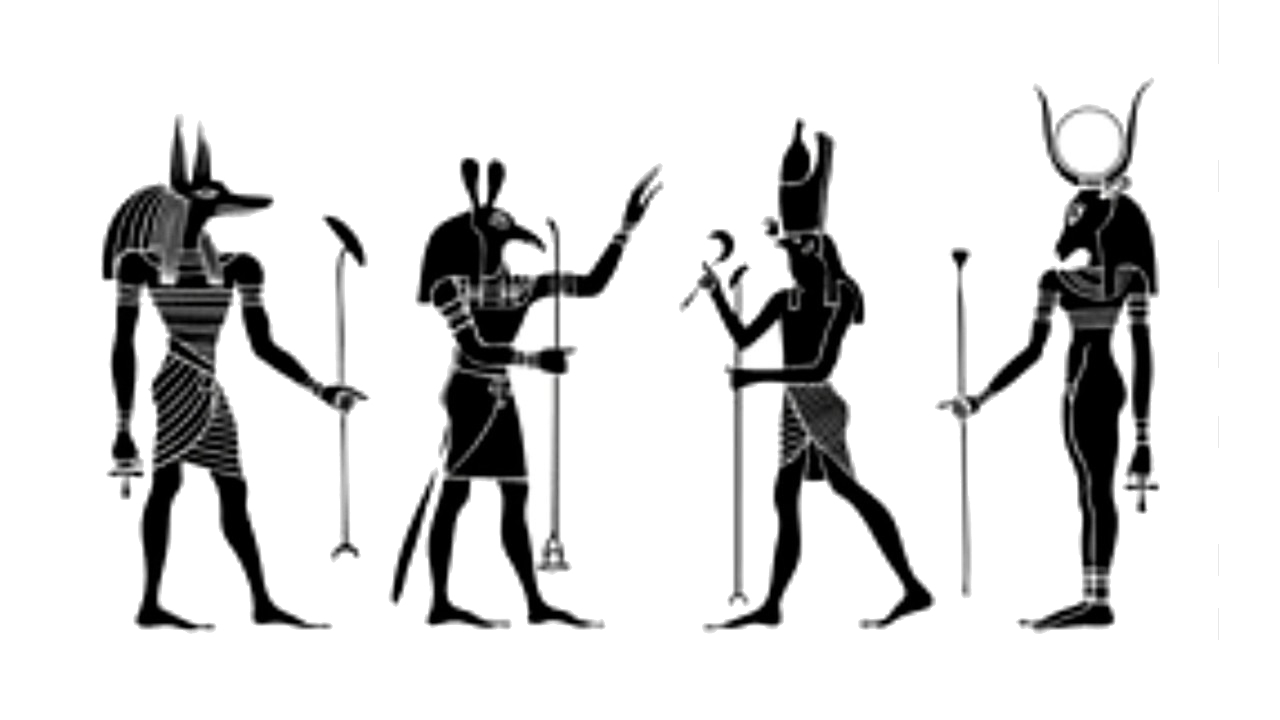
\includegraphics[width=5.75cm]{../resources/jpg/2.2.set.operations/set.jpg}
\end{figure}


% ============================== 0018 Theorem 2205 ================================
\subsection[The set complementation law.]
    {
        \color{section}Theorem 18 \color{black} : the set complementation law.
    }
\documentclass[preview]{standalone}
\usepackage{amssymb, amsthm}
\usepackage{mathtools}
\usepackage{bm}


\newtheorem{theorem}{Theorem}
\renewcommand\qedsymbol{$\blacksquare$}


\begin{document}


\begin{theorem} %[\textbf{2205}] \color{black}
    Let \bm{$\Lambda$} be a subset of \space \bm{$\Omega$}.
    \bm{$\overline{\overline{\Lambda}} = \Lambda$}.
\end{theorem}
\begin{proof} \color{black}
    Suppose there exists an element \bm{$\chi$} such that \bm{$\chi$} is a member of 
    \bm{$\overline{\overline{\Lambda}}$}. 
    By the definition for set complementation, 
    and by the defintion for set membership, 
    that is 
    \begin{equation*}
        \Big \langle \chi \in \overline{\overline{\Lambda}} \Big \rangle 
            \equiv
        \Big \langle \chi \notin \overline{\Lambda} \Big \rangle 
            \equiv
        \lnot \Big \langle \chi \in \overline{\Lambda} \Big \rangle 
            \equiv
        \lnot \Big \langle \chi \notin \Lambda \Big \rangle 
            \equiv
        \lnot \Big \langle \lnot \big \langle \chi \in \Lambda \big \rangle \Big \rangle
    \end{equation*}
    By the logical law of double negation, $\bm{\chi \in \Lambda}$.
    Since logical equivalence is biconditional by definition, 
    this sequence of equivalencies proves both, that 
    \begin{equation*}
        \Big \langle 
            \overline{\overline{\Lambda}}
                \subseteq 
            \Lambda
        \Big \rangle 
            \land 
        \Big \langle 
            \Lambda
                \subseteq 
            \overline{\overline{\Lambda}}
        \Big \rangle
    \end{equation*}
    $\therefore \text{\space} \bm{\overline{\overline{\Lambda}} = \Lambda$}; 
    the complementation law for sets.
\end{proof}


\end{document}
\pagebreak


% ============================= 0019 Theorem 2206a ================================
\subsection[The identity law for set union.]
    {
        \color{section}Theorem 19 \color{black} : the identity law for set union.
    }
\documentclass[preview]{standalone}
\usepackage{amssymb, amsthm}
\usepackage{mathtools}
\usepackage{bm}


\newtheorem{theorem}{Theorem}
\renewcommand\qedsymbol{$\blacksquare$}


\begin{document}


\begin{theorem} %[\textbf{2206a}]
    Let \bm{$\Xi$} be a set. 
    The set identity for \bm{$\Xi$} is \bm{$\Xi \cup \varnothing = \Xi$}.
\end{theorem}
\begin{proof}
    Suppose there exists an element \bm{$\zeta$} such that \bm{$\zeta$} is a member of 
    \bm{$\Xi \cup \varnothing$}. 
    By the definition of set union, that is 
    \begin{equation*}
        \Big \langle \zeta \in \Xi \Big \rangle 
            \lor 
        \Big \langle \zeta \in \varnothing \Big \rangle
    \end{equation*}
    The logical identity for the statement \bm{$\zeta \in \varnothing$} is trivially \bm{$\bot$}, 
    because the empty set contains no members. 
    Thus, by that identity, and by the identity law for logical disjunction,
    \begin{equation*} 
        \Bigg\{
            \Big \langle \zeta \in \Xi \Big \rangle 
                \lor 
            \Big \langle \zeta \in \varnothing \Big \rangle
        \Bigg\} 
            \equiv
        \Bigg\{
            \Big \langle \zeta \in \Xi \Big \rangle 
                \lor
            \Big \langle \bot \Big \rangle 
                \equiv
            \Big \langle \zeta \in \Xi \Big \rangle
        \Bigg\}
            \equiv
    \end{equation*}
    \begin{equation*} 
        \Bigg\{
            \Big \langle \zeta \in \Xi \Big \rangle 
                \lor 
            \Big \langle \zeta \in \varnothing \Big \rangle
                \equiv
            \Big \langle \zeta \in \Xi \Big \rangle
        \Bigg\}
    \end{equation*}
    $\therefore$ 
    by the definition for set union,
    the set identity for \bm{$\Xi$} is \bm{$\Xi \cup \varnothing = \Xi$}.
\end{proof}


\end{document}
\sep


% ============================= 0020 Theorem 2206b ================================
\subsection[The identity law for set intersection.]
    {
        \color{section}Theorem 20 \color{black} : the identity law for set intersection.
    }
\documentclass[preview]{standalone}
\usepackage{amssymb, amsthm}
\usepackage{mathtools}
\usepackage{bm}


\newtheorem*{theorem*}{Theorem}
\renewcommand\qedsymbol{$\blacksquare$}


\begin{document}


\begin{theorem} %[\textbf{2206b}]
    Let \bm{$\Xi$} be a set with universal set \bm{$\Omega$}. 
    The set identity for \bm{$\Xi$} is \bm{$\Xi \cap \Omega = \Xi$}.
\end{theorem}
\begin{proof}
    Suppose there exists an element \bm{$\zeta$} such that \bm{$\zeta$} is a member of \bm{$\Xi \cap \Omega$}. 
    By the definition for set intersection, that is
    \begin{equation*}
        \Big \langle \zeta \in \Xi \Big \rangle 
            \land 
        \Big \langle \zeta \in \Omega \Big \rangle
    \end{equation*}
    The logical identity for the statement \bm{$\zeta \in \Omega$} is trivially \bm{$\top$}, 
    because \bm{$\Omega$} is the universe. 
    Thus, by that identity, and by the identity law for logical conjunction, 
    \begin{equation*}
        \Bigg\{
            \Big \langle \zeta \in \Xi \Big \rangle 
                \land 
            \Big \langle \zeta \in \Omega \Big \rangle 
        \Bigg\} 
            \equiv
        \Bigg\{
            \Big \langle \zeta \in \Xi \Big \rangle 
                \land 
            \Big \langle \top \Big \rangle 
                \equiv 
            \Big \langle \zeta \in \Xi \Big \rangle
        \Bigg\}
            \equiv
    \end{equation*}
    \begin{equation*}
        \Bigg\{
            \Big \langle \zeta \in \Xi \Big \rangle 
                \land 
            \Big \langle \zeta \in \Omega \Big \rangle
                \equiv
            \Big \langle \zeta \in \Xi \Big \rangle
        \Bigg\}
    \end{equation*}
    $\therefore$ by the definition for the intersection of sets,
    the set identity for \bm{$\Xi$} is \bm{$\Xi \cap \Omega = \Xi$}.
\end{proof}


\end{document}
\pagebreak


% ============================= 0021 Theorem 2207a ================================
\subsection[Domination for set union.]
    {
        \color{section}Theorem 21 \color{black} : domination for set union.
    }
\documentclass[preview]{standalone}
\usepackage{amssymb, amsthm}
\usepackage{mathtools}
\usepackage{bm}


\newtheorem{theorem}{Theorem}
\renewcommand\qedsymbol{$\blacksquare$}


\begin{document}


\begin{theorem} %[\textbf{2207a}]
    Let \bm{$\Xi$} be a set with universal set \bm{$\Omega$}. 
    \bm{$\Omega$} dominates set union such that 
    \begin{equation*}
        \bm{\Xi \cup \Omega = \Omega}    
    \end{equation*}
\end{theorem}
\begin{proof}
    Suppose there exists an element \bm{$\zeta$} such that \bm{$\zeta$} is a member of 
    \bm{$\Xi \cup \Omega$}. 
    By the definition for set union, that is
    \begin{equation*}
        \Big \langle \zeta \in \Xi \Big \rangle
            \lor 
        \Big \langle \zeta \in \Omega \Big \rangle
    \end{equation*}
    The logical identity for the statement \bm{$\zeta \in \Omega$} is trivially \bm{$\top$}, 
    since \bm{$\Omega$} is the universe. 
    Thus, 
    by that identity, 
    and by the domination law for logical disjunction,
    \begin{equation*}
        \Bigg\{
            \Big \langle \zeta \in \Xi \Big \rangle 
                \lor 
            \Big \langle \zeta \in \Omega \Big \rangle
        \Bigg\}
            \equiv
        \Bigg\{
            \Big \langle \zeta \in \Xi \Big \rangle 
                \lor 
            \Big \langle \top \Big \rangle
                \equiv
            \Big \langle \zeta \in \Omega \Big \rangle
        \Bigg\}
            \equiv
    \end{equation*}
    \begin{equation*}
        \Bigg\{
            \Big \langle \zeta \in \Xi \Big \rangle 
                \lor 
            \Big \langle \zeta \in \Omega \Big \rangle
                \equiv
            \Big \langle \zeta \in \Omega \Big \rangle
        \Bigg\}
    \end{equation*}
    $\therefore$ by the definition for the union of sets, 
    \bm{$\Omega$} dominates set union such that 
    \bm{$\Xi \cup \Omega = \Omega$}.
\end{proof}


\end{document}
\sep
\begin{figure}[!h]
    \centering
    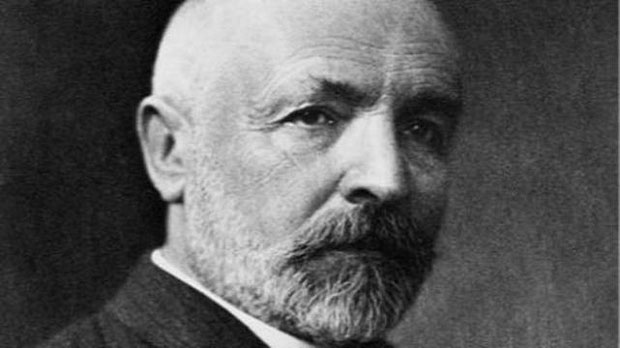
\includegraphics[width=13.75cm]{../resources/jpg/2.2.set.operations/georg_cantor.jpg}
    \caption*{Georg Cantor.}
\end{figure}
\pagebreak


% ============================= 0022 Theorem 2207b ================================
\subsection[Domination for set intersection.]
    {
        \color{section}Theorem 22 \color{black} : domination for set intersection.
    }
\documentclass[preview]{standalone}
\usepackage{amssymb, amsthm}
\usepackage{mathtools}
\usepackage{bm}


\newtheorem{theorem}{Theorem}
\renewcommand\qedsymbol{$\blacksquare$}


\begin{document}


\begin{theorem} %[\textbf{2207b}]
    Let \bm{$\Xi$} be a set. 
    The empty set dominates set intersection such that
    \begin{equation*}
        \bm{\Xi \cap \varnothing = \varnothing}
    \end{equation*}
\end{theorem}
\begin{proof}
    Let \bm{$\zeta$} be an element in \bm{$\Xi \cap \varnothing$}. 
    By the definition for set intersection, that is 
    \begin{equation*}
        \Big \langle \zeta \in \Xi \Big \rangle 
            \land 
        \Big \langle \zeta \in \varnothing \Big \rangle
    \end{equation*}
    The logical identity for the statement \bm{$\zeta \in \varnothing$} is trivially \bm{$\bot$}, 
    since the empty set contains no members. 
    Thus, by that identity, 
    and by the domination law for logical conjunction,
    \begin{equation*}
        \Bigg\{
            \Big \langle \zeta \in \Xi \Big \rangle 
                \land 
            \Big \langle \zeta \in \varnothing \Big \rangle
        \Bigg\}
            \equiv
        \Bigg\{
            \Big \langle \zeta \in \Xi \Big \rangle 
                \land 
            \Big \langle \bot \Big \rangle
                \equiv
            \Big \langle \zeta \in \varnothing \Big \rangle
        \Bigg\}
            \equiv
    \end{equation*}
    \begin{equation*}
        \Bigg\{
            \Big \langle \zeta \in \Xi \Big \rangle 
                \land 
            \Big \langle \zeta \in \varnothing \Big \rangle
                \equiv
            \Big \langle \zeta \in \varnothing \Big \rangle
        \Bigg\}
    \end{equation*}
    $\therefore$ by the definition for the intersection of sets,
    the empty set dominates set intersection such that 
    \bm{$\Xi \cap \varnothing = \varnothing$}.
\end{proof}


\end{document}
\vspace{3\baselineskip}
\begin{figure}[!h]
    \centering
    
\includegraphics[width=6cm]{../resources/jpg/2.2.set.operations/border1.jpg}
\end{figure}
\vspace{2\baselineskip}


% ============================= 0023 Theorem 2208a ================================
\subsection[Idempotence for the union of sets.]
    {
        \color{section}Theorem 23 \color{black} : idempotence for the union of sets.
    }
\documentclass[preview]{standalone}
\usepackage{amssymb, amsthm}
\usepackage{mathtools}
\usepackage{bm}


\newtheorem{theorem}{Theorem}
\renewcommand\qedsymbol{$\blacksquare$}


\begin{document}


\begin{theorem} %[\textbf{2208a}]
    Let \bm{$\Lambda$} be a set. 
    \bm{$\Lambda$} is idempotent such that 
    \bm{$\Lambda \cup \Lambda = \Lambda$}.
\end{theorem}
\begin{proof}
    Let \bm{$\mu$} be an element in \bm{$\Lambda \cup \Lambda$}. 
    By the definition of set union, that is 
    \begin{equation*}
        \Big \langle \mu \in \Lambda \Big \rangle 
            \lor 
        \Big \langle \mu \in \Lambda \Big \rangle
    \end{equation*}
    Thus, by the idempotent law for logical disjunction, 
    \begin{equation*}
        \Big \langle \mu \in \Lambda \Big \rangle 
            \lor 
        \Big \langle \mu \in \Lambda \Big \rangle 
            \equiv 
        \Big \langle \mu \in \Lambda \Big \rangle
    \end{equation*}
    $\therefore$ by the defintion for set union,
    \bm{$\Lambda$} is idempotent such that 
    \bm{$\Lambda \cup \Lambda = \Lambda$}.
\end{proof}


\end{document}
\pagebreak


% ============================= 0024 Theorem 2208b ================================
\subsection[Idempotence for the intersection of sets.]
    {
        \color{section}Theorem 24 \color{black} : idempotence for the intersection of sets.
    }
\documentclass[preview]{standalone}
\usepackage{amssymb, amsthm}
\usepackage{mathtools}
\usepackage{bm}


\newtheorem{theorem}{Theorem}
\renewcommand\qedsymbol{$\blacksquare$}


\begin{document}


\begin{theorem} %[\textbf{2208b}]
    Let \bm{$\Lambda$} be a set.
    \bm{$\Lambda$} is idempotent such that 
    \bm{$\Lambda \cap \Lambda = \Lambda$}.
\end{theorem}
\begin{proof}
    Let \bm{$\mu$} be an element in \bm{$\Lambda \cap \Lambda$}. 
    By the definition for set intersection,
    \begin{equation*}
        \Big \langle \mu \in \Lambda \Big \rangle 
            \land 
        \Big \langle \mu \in \Lambda \Big \rangle
    \end{equation*}
    Thus, by the idempotent law for logical conjunction,
    \begin{equation*}
        \Big \langle \mu \in \Lambda \Big \rangle 
            \land 
        \Big \langle \mu \in \Lambda \big \rangle 
            \equiv 
        \Big \langle \mu \in \Lambda \Big \rangle
    \end{equation*}
    $\therefore$ by the definition for the intersection of sets,
    \bm{$\Lambda$} is idempotent such that 
    \bm{$\Lambda \cap \Lambda = \Lambda$}.
\end{proof}


\end{document}
\sep


% ============================= 0025 Theorem 2209a ================================
\subsection[The complement law for set union.]
    {
        \color{section}Theorem 25 \color{black} : the complement law for set union.
    }
\documentclass[preview]{standalone}
\usepackage{amssymb, amsthm}
\usepackage{mathtools}
\usepackage{bm}


\newtheorem{theorem}{Theorem}
\renewcommand\qedsymbol{$\blacksquare$}


\begin{document}


\begin{theorem}[\textbf{2209a}]
    Let \bm{$\Psi$} be a set with universal set \bm{$\Omega$}.
    \bm{$\Psi \cup \overline{\Psi} = \Omega$}.
\end{theorem}
\begin{proof}
    Let \bm{$\sigma$} be an element in \bm{$\Psi \cup \overline{\Psi}$}. 
    By the definition for set union,  
    \begin{equation*}
        \Big \langle \sigma \in \Psi \Big \rangle 
            \lor 
        \Big \langle \sigma \in \overline{\Psi} \Big \rangle
    \end{equation*}
    The right-hand side of this disjunction is equivalent to \bm{$\sigma \in \Omega - \Psi$}, 
    by the definition for set complementation. 
    By Theorem 45, \bm{$\sigma \in \Omega \cap \overline{\Psi}$}, 
    which is defined as 
    \bm{$\big \langle \sigma \in \Omega \big \rangle 
        \land 
    \big \langle \sigma \notin \Psi \big \rangle$},
    by the definitions for set intersection and set complementation. 
    Thus, the original disjunction is the same as 
    \begin{equation*}
        \Big \langle \sigma \in \Psi \Big \rangle 
            \lor 
        \Bigg[
            \Big \langle \sigma \in \Omega \Big \rangle 
                \land 
            \Big \langle \sigma \notin \Psi \Big \rangle
        \Bigg]
    \end{equation*}
    We must distribute the left-hand side of this disjunction over the conjunction occurring in the right-hand side. 
    We get 
    \begin{equation*}
        \Bigg[
            \Big \langle \sigma \in \Psi \Big \rangle 
                \lor 
            \Big \langle \sigma \in \Omega \Big \rangle
        \Bigg] 
            \land 
        \Bigg[
            \Big \langle \sigma \in \Psi \Big \rangle 
                \lor 
            \Big \langle \sigma \notin \Psi \Big \rangle
        \Bigg]
    \end{equation*}
    By the logical law of negation, 
    the identity for the right-hand side of this conjunction is \bm{$\top$}. 
    The left-hand side of this conjunction is dominated by \bm{$\Omega$}, 
    according to Theorem 21. 
    Therefore, 
    the statement \bm{$\sigma \in \Psi \cup \overline{\Psi}$} can be equivalently stated as 
    \bm{$\big \langle \sigma \in \Omega \big \rangle \land \top$}; 
    the logical identity for which is \bm{$\sigma \in \Omega$}. 
    The converse trivially follows from the fact of logical equivalence. 
    Thus, 
    proves the set complement law for the union of sets, 
    \bm{$\Psi \cup \overline{\Psi} = \Omega$}.
\end{proof}


\end{document}
\pagebreak


% ============================= 0026 Theorem 2209b ================================
\subsection[The complement law for set intersection.]
    {
        \color{section}Theorem 26 \color{black} : the complement law for set intersection.
    }
\documentclass[preview]{standalone}
\usepackage{amssymb, amsthm}
\usepackage{mathtools}
\usepackage{bm}


\newtheorem{theorem}{Theorem}
\renewcommand\qedsymbol{$\blacksquare$}


\begin{document}


\begin{theorem}[\textbf{2209b}]
    Let \bm{$\Xi$} be a set. 
    \bm{$\Xi \cap \overline{\Xi} = \varnothing$}.
\end{theorem}
\begin{proof}
    Let \bm{$\zeta$} be an element in \bm{$\Xi \cap \overline{\Xi}$}. 
    By the definition for the intersection of sets, that is
    \begin{equation*}
        \Big \langle \zeta \in \Xi \Big \rangle 
            \land 
        \Big \langle \zeta \in \overline{\Xi} \Big \rangle
    \end{equation*} 
    According to the definitions for set complementation and set membership, 
    and by the negation law of logic, that is
    \begin{equation*}
        \Bigg\{
            \Big \langle \zeta \in \Xi \Big \rangle 
                \land 
            \Big \langle \zeta \in \overline{\Xi} \Big \rangle
        \Bigg\}
            \equiv
        \Bigg\{
            \Big \langle \zeta \in \Xi \Big \rangle 
                \land 
            \lnot \Big \langle \zeta \in \Xi \Big \rangle
                \equiv
            \Big \langle \bot \Big \rangle
        \Bigg\}
    \end{equation*}
    \bm{$\big \langle \bot \big \rangle$} is trivially the logical identity for 
    the statement \bm{$\zeta \in \varnothing$}, 
    since the empty set contains no members. 
    Thus, 
    by that identity, 
    and following from the series of equivalencies from above,
    \begin{equation*}
        \Big \langle \zeta \in \Xi \Big \rangle 
            \land 
        \Big \langle \zeta \in \overline{\Xi} \Big \rangle 
            \equiv
        \Big \langle \zeta \in \varnothing \Big \rangle
    \end{equation*}
    $\therefore$ the complement law for sets, 
    \bm{$\Xi \cap \overline{\Xi} = \varnothing$}, 
    follows immediately from the definition for the intersection of sets.
\end{proof}


\end{document}
\sep


% ============================= 0027 Theorem 2210a ===============================
\subsection[Subtracting the empty set.]
    {
        \color{section}Theorem 27 \color{black} : subtracting the empty set.
    }
\documentclass[preview]{standalone}
\usepackage{amssymb, amsthm}
\usepackage{mathtools}
\usepackage{bm}


\newtheorem{theorem}{Theorem}
\renewcommand\qedsymbol{$\blacksquare$}


\begin{document}


\begin{theorem}[\textbf{2210a}]
    Let \bm{$\Xi$} be a set. 
    \bm{$\Xi - \varnothing = \Xi$}.
\end{theorem}
\begin{proof}
    Suppose there exists an element \bm{$\zeta$} such that \bm{$\zeta$} is a member of 
    \bm{$\Xi - \varnothing$}.
    By the definition for set difference, that is
    \begin{equation*}
        \Big \langle \zeta \in \Xi \Big \rangle
            \land 
        \Big \langle \zeta \notin \varnothing \Big \rangle
    \end{equation*}
    It is trivial that the logical identity for the statement 
    \bm{$\zeta \notin \varnothing$} is \bm{$\top$},
    since the empty set contains no members. 
    Thus, by that identity, 
    and by the identity law for logical conjunction,
    \begin{equation*}
        \Bigg\{
            \Big \langle \zeta \in \Xi \Big \rangle
                \land 
            \Big \langle \zeta \notin \varnothing \Big \rangle
        \Bigg\}
            \equiv
        \Bigg\{
            \Big \langle \zeta \in \Xi \Big \rangle
                \land 
            \Big \langle \top \Big \rangle
                \equiv
            \Big \langle \zeta \in \Xi \Big \rangle
        \Bigg\}
            \equiv
    \end{equation*}
    \begin{equation*}
        \Bigg\{
            \Big \langle \zeta \in \Xi \Big \rangle
                \land 
            \Big \langle \zeta \notin \varnothing \Big \rangle
                \equiv
            \Big \langle \zeta \in \Xi \Big \rangle
        \Bigg\}
    \end{equation*}
    $\therefore$ by the definition for set difference,
    \bm{$\Xi - \varnothing = \Xi$}.
\end{proof}


\end{document}
\pagebreak


% ============================= 0028 Theorem 2210b ===============================
\subsection[The empty set minus any set is empty.]
    {
        \color{section}Theorem 28 \color{black} : the empty set minus any set is empty.
    }
\documentclass[preview]{standalone}
\usepackage{amssymb, amsthm}
\usepackage{mathtools}
\usepackage{bm}


\newtheorem{theorem}{Theorem}
\renewcommand\qedsymbol{$\blacksquare$}


\begin{document}


\begin{theorem}[\textbf{2210b}]
    Let \bm{$\Xi$} be a set. 
    \bm{$\varnothing - \Xi = \varnothing$}.
\end{theorem}
\begin{proof}
    Let \bm{$\zeta$} be an element in \bm{$\varnothing - \Xi$}. 
    By the definition for set difference,
    \begin{equation*}
        \Big \langle \zeta \in \varnothing \Big \rangle
            \land 
        \Big \langle \zeta \notin \Xi \Big \rangle
    \end{equation*}
    The logical identity for the statement \bm{$\zeta \in \varnothing$} is trivially \bm{$\bot$}, 
    since the empty set contains no members. 
    Thus, by that identity, and by the domination law for logical conjunction,
    \begin{equation*}
        \Bigg\{
            \Big \langle \zeta \in \varnothing \Big \rangle
                \land 
            \Big \langle \zeta \notin \Xi \Big \rangle
        \Bigg\}
            \equiv
        \Bigg\{
            \Big \langle \bot \Big \rangle
                \land 
            \Big \langle \zeta \notin \Xi \Big \rangle 
                \equiv 
            \Big \langle \bot \Big \rangle
        \Bigg\}
            \equiv
    \end{equation*}
    \begin{equation*}
        \Bigg\{
            \Big \langle \zeta \in \varnothing \Big \rangle
                \land 
            \Big \langle \zeta \notin \Xi \Big \rangle
                \equiv
            \Big \langle \zeta \in \varnothing \Big \rangle
        \Bigg\}
    \end{equation*}
    $\therefore$ by the definition for set difference,  
    \bm{$\varnothing - \Xi = \varnothing$}
\end{proof}


\end{document}
\vspace{2.9\baselineskip}
\begin{figure}[!h]
    \centering
    
\includegraphics[width=8cm]{../resources/jpg/2.2.set.operations/border2.jpg}
\end{figure}
\vspace{2\baselineskip}


% ============================= 0029 Theorem 2211a ===============================
\subsection[Set union is commutative.]
    {
        \color{section}Theorem 29 \color{black} : set union is commutative.
    }
\documentclass[preview]{standalone}
\usepackage{amssymb, amsthm}
\usepackage{mathtools}
\usepackage{bm}


\newtheorem{theorem}{Theorem}
\renewcommand\qedsymbol{$\blacksquare$}


\begin{document}


\begin{theorem}[\textbf{2211a}]
    Let \bm{$\mathrm{A}$} and \bm{$\Lambda$} be sets. 
    The union of \bm{$\mathrm{A}$} and \bm{$\Lambda$} is commutative.
\end{theorem}
\begin{proof}
    Let \bm{$\lambda$} be an element in \bm{$\mathrm{A} \cup \Lambda$}. 
    By the definition for set union,
    \begin{equation*}
        \Big \langle \lambda \in \mathrm{A} \Big \rangle 
            \lor 
        \Big \langle \lambda \in \Lambda \Big \rangle
    \end{equation*} 
    Because logical disjunction is commutative, 
    that is 
    \begin{equation*}
        \Bigg[
            \Big \langle \lambda \in \mathrm{A} \Big \rangle
                \lor 
            \Big \langle \lambda \in \Lambda \Big \rangle
        \Bigg]
            \equiv 
        \Bigg[
            \Big \langle \lambda \in \Lambda \Big \rangle
                \lor 
            \Big \langle \lambda \in \mathrm{A} \Big \rangle
        \Bigg]
    \end{equation*} 
    $\therefore \text{\space} 
    \bm{\mathrm{A} \cup \Lambda = \Lambda \cup \mathrm{A}$}, 
    and the union of \bm{$\mathrm{A}$} and \bm{$\Lambda$} is indeed commutative.
\end{proof}


\end{document}
\pagebreak


% ============================= 0030 Theorem 2211b ===============================
\subsection[Set intersection is commutative.]
    {
        \color{section}Theorem 30 \color{black} : set intersection is commutative.
    }
\documentclass[preview]{standalone}
\usepackage{amssymb, amsthm}
\usepackage{mathtools}
\usepackage{bm}


\newtheorem{theorem}{Theorem}
\renewcommand\qedsymbol{$\blacksquare$}


\begin{document}


\begin{theorem}[\textbf{2211b}]
    Let \bm{$\mathrm{A}$} and \bm{$\Lambda$} be sets. 
    The intersection of \bm{$\mathrm{A}$} and \bm{$\Lambda$} is commutative.
\end{theorem}
\begin{proof}
    Let \bm{$\lambda$} be an element in \bm{$\mathrm{A} \cap \Lambda$}. 
    By the definition for set intersection, 
    \begin{equation*}
        \Big \langle \lambda \in \mathrm{A} \Big \rangle 
            \land 
        \Big \langle \lambda \in \Lambda \Big \rangle
    \end{equation*}
    Because logical conjunction is commutative, that is
    \begin{equation*}
        \Bigg[
            \Big \langle \lambda \in \mathrm{A} \Big \rangle 
                \land 
            \Big \langle \lambda \in \Lambda \Big \rangle
        \Bigg]
            \equiv
        \Bigg[
            \Big \langle \lambda \in \Lambda \Big \rangle 
                \land 
            \Big \langle \lambda \in \mathrm{A} \Big \rangle
        \Bigg]
    \end{equation*}
    $\therefore \text{\space} 
    \bm{\mathrm{A} \cap \Lambda = \Lambda \cap \mathrm{A}}$, 
    and indeed the intersection of \bm{$\mathrm{A}$} and \bm{$\Lambda$} is commutative.
\end{proof}


\end{document}
\vspace{2.9\baselineskip}
\begin{figure}[!h]
    \centering
    
\includegraphics[width=7cm]{../resources/jpg/2.2.set.operations/border3.jpg}
\end{figure}
\vspace{2.8\baselineskip}

% ============================= 0031 Theorem 2212 ================================
\subsection[Absorption for union over intersection.]
    {
        \color{section}Theorem 31 \color{black} : absorption for union over intersection.
    }
\documentclass[preview]{standalone}
\usepackage{amssymb, amsthm}
\usepackage{mathtools}
\usepackage{bm}


\newtheorem{theorem}{Theorem}
\renewcommand\qedsymbol{$\blacksquare$}


\begin{document}


\begin{theorem}[\textbf{2212}]
    Let \bm{$\mathrm{A}$} and \bm{$\Lambda$} be sets. 
    \bm{$
    \mathrm{A} 
        \cup 
    \big \langle \mathrm{A} \cap \Lambda \big \rangle 
        = 
    \mathrm{A}$}.
\end{theorem}
\begin{proof}
    Let \bm{$\lambda$} be an element in 
    \bm{$
    \mathrm{A} 
        \cup 
    \big \langle \mathrm{A} \cap \Lambda \big \rangle
    $}. 
    By the definitions for the union of sets and the intersection of sets, that is
    \begin{equation*}
        \Big \langle \lambda \in \mathrm{A} \Big \rangle 
            \lor 
        \bigg[
            \Big \langle \lambda \in \mathrm{A} \Big \rangle 
                \land 
            \Big \langle \lambda \in \Lambda \Big \rangle
        \bigg]
    \end{equation*}
    It follows immediately from the laws of logical absorption that
    \begin{equation*}
        \Bigg\{
            \Big \langle \lambda \in \mathrm{A} \Big \rangle 
                \lor 
            \bigg[
                \Big \langle \lambda \in \mathrm{A} \Big \rangle 
                    \land 
                \Big \langle \lambda \in \Lambda \Big \rangle
            \bigg]
        \Bigg\}
            \equiv 
        \bigg \langle \lambda \in \mathrm{A} \bigg \rangle 
    \end{equation*}
    $\therefore$ by the definitions for set union and set intersection, 
    \bm{$
    \mathrm{A} 
        \cup 
    \big \langle \mathrm{A} \cap \Lambda \big \rangle 
        = 
    \mathrm{A}$}; 
    the absorption law for set union over intersection.
\end{proof}


\end{document}
\pagebreak


% ============================= 0032 Theorem 2213 ================================
\subsection[Absorption for intersection over union.]
    {
        \color{section}Theorem 32 \color{black} : absorption for intersection over union.
    }
\documentclass[preview]{standalone}
\usepackage{amssymb, amsthm}
\usepackage{mathtools}
\usepackage{bm}


\newtheorem{theorem}{Theorem}
\renewcommand\qedsymbol{$\blacksquare$}


\begin{document}


\begin{theorem}[\textbf{2213}]
    Let \bm{$\mathrm{A}$} and \bm{$\Lambda$} be sets. 
    \bm{$
    \mathrm{A} 
        \cap 
    \big \langle \mathrm{A} \cup \Lambda \big \rangle 
        = 
    \mathrm{A}
    $}.
\end{theorem}
\begin{proof}
    Let \bm{$\lambda$} be an element in 
    \bm{$
    \mathrm{A} 
        \cap 
    \big \langle \mathrm{A} \cup \Lambda \big \rangle
    $}. 
    By the definitions for set union and set intersection, that is 
    \begin{equation*}
        \Big \langle \lambda \in \mathrm{A} \Big \rangle 
            \land 
        \bigg[
            \Big \langle \lambda \in \mathrm{A} \Big \rangle 
                \lor 
            \Big \langle \lambda \in \Lambda \Big \rangle
        \bigg]
    \end{equation*}
    It follows immediately from the laws of logical absorption that
    \begin{equation*}
        \Bigg\{
            \Big \langle \lambda \in \mathrm{A} \Big \rangle 
                \land 
            \bigg[
                \Big \langle \lambda \in \mathrm{A} \Big \rangle 
                    \lor 
                \Big \langle \lambda \in \Lambda \Big \rangle
            \bigg]
        \Bigg\}
            \equiv
        \bigg \langle \lambda \in \mathrm{A} \bigg \rangle 
    \end{equation*}
    $\therefore$ by the definitions for set intersection and set union, 
    \bm{$
    \mathrm{A} 
        \cap 
    \big \langle \mathrm{A} \cup \Lambda \big \rangle 
        = 
    \mathrm{A}
    $}; 
    the absorption law for set intersection over union. 
\end{proof}


\end{document}
\vspace{1.1\baselineskip}
\begin{figure}[!h]
    \centering
    
\includegraphics[width=9cm]{../resources/jpg/2.2.set.operations/border4.jpg}
\end{figure}
\vspace{.1\baselineskip}


% ============================= 0033 Theorem 2215 ================================
\subsection[DeMorgan's Law for a complemented union.]
    {
        \color{section}Theorem 33 \color{black} : DeMorgan's for complemented unions.
    }
\documentclass[preview]{standalone}
\usepackage{amssymb, amsthm}
\usepackage{mathtools}
\usepackage{bm}


\newtheorem{theorem}{Theorem}
\renewcommand\qedsymbol{$\blacksquare$}


\begin{document}


\begin{theorem}[\textbf{2215}]
    Let \bm{$\mathrm{A}$} and \bm{$\Lambda$} be sets. 
    \bm{$
    \overline{\mathrm{A} \cup \Lambda} 
        = 
    \overline{\mathrm{A}} \cap \overline{\Lambda}
    $}.
\end{theorem}
\begin{proof}
    Let \bm{$\lambda$} be an element in \bm{$\overline{\mathrm{A} \cup \Lambda}$}. 
    By the definitions for set complementation, and set membership, that is 
    \bm{$\lnot 
            \Big[
                \lambda \in \big \langle \mathrm{A} \cup \Lambda \big \rangle 
            \Big]
    $}. 
    Hence, by the definition of set union, 
    \begin{equation*}
        \lnot \bigg[
            \Big \langle \lambda \in \mathrm{A} \Big \rangle 
                \lor 
            \Big \langle \lambda \in \Lambda \Big \rangle
        \bigg]    
    \end{equation*}
    By DeMorgans law (from logic), 
    and by the definitions for set complementation
    and set membership
    \begin{equation*}
        \Bigg\{
            \lnot \bigg[
                \Big \langle \lambda \in \mathrm{A} \Big \rangle 
                    \lor 
                \Big \langle \lambda \in \Lambda \Big \rangle
            \bigg]
        \Bigg\}
        \equiv
        \Bigg\{
            \lnot \Big \langle \lambda \in \mathrm{A} \Big \rangle 
                \land 
            \lnot \Big \langle \lambda \in \Lambda \Big \rangle
        \Bigg\}
        \equiv
    \end{equation*}
    \begin{equation*}
        \Bigg\{
            \Big \langle \lambda \in \overline{\mathrm{A}} \Big \rangle 
                \land 
            \Big \langle \lambda \in \overline{\Lambda} \Big \rangle
        \Bigg\}
    \end{equation*}
    $\therefore$ by the definition of set intersection,
    \bm{$
    \overline{\mathrm{A} \cup \Lambda} 
        = 
    \overline{\mathrm{A}} \cap \overline{\Lambda}
    $};
    DeMorgans law for sets.
\end{proof}


\end{document}
\pagebreak


% ============================= 0034 Theorem 2216a ===============================
\subsection[Intersection is a subset of its operands.]
    {
        \color{section}Theorem 34 \color{black} : intersection is a subset of its operands.
    }
\documentclass[preview]{standalone}
\usepackage{amssymb, amsthm}
\usepackage{mathtools}
\usepackage{bm}


\newtheorem{theorem}{Theorem}
\renewcommand\qedsymbol{$\blacksquare$}


\begin{document}


\begin{theorem}[\textbf{2216a}]
    Let \bm{$\mathrm{A}$} and \bm{$\Lambda$} be sets. 
    \bm{$
    \big \langle \mathrm{A} \cap \Lambda \big \rangle 
        \subseteq 
    \mathrm{A}
    $}.
\end{theorem}
\begin{proof}
    Let \bm{$\lambda$} be an element in \bm{$\mathrm{A} \cap \Lambda$}. 
    By the definition for set intersection,
    \begin{equation*}
        \Big \langle \lambda \in \mathrm{A} \Big \rangle 
            \land 
        \Big \langle \lambda \in \Lambda \Big \rangle   
    \end{equation*}
    It trivially follows from the simplification rule of inference that 
    \begin{equation*}
        \bigg[
            \Big \langle \lambda \in \mathrm{A} \Big \rangle 
                \land 
            \Big \langle \lambda \in \Lambda \Big \rangle
        \bigg]
            \rightarrow
        \Big \langle \lambda \in \mathrm{A} \Big \rangle
    \end{equation*}
    $\therefore$ 
    \bm{$
    \big \langle \mathrm{A} \cap \Lambda \big \rangle 
        \subseteq 
    \mathrm{A}
    $}, by the definition of subsets.
\end{proof}


\end{document}
\vspace{2\baselineskip}
\begin{figure}[!h]
    \centering
    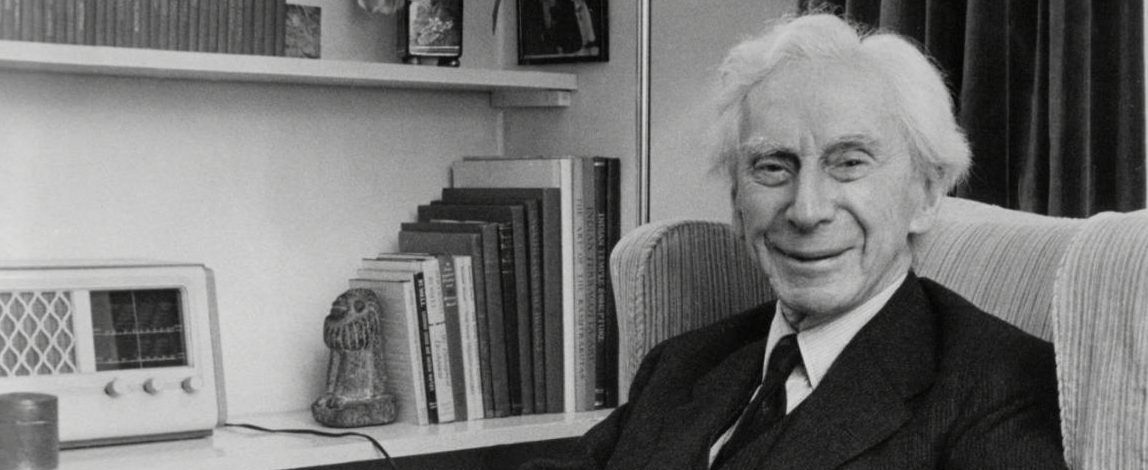
\includegraphics[width=14cm]{../resources/jpg/2.2.set.operations/russel.jpg}
    \caption*{Bertrand Russel.}
\end{figure}


% ============================= 0035 Theorem 2216b ===============================
\subsection[A set is a subset of its union.]
    {
        \color{section}Theorem 35 \color{black} : a set is a subset of its union.
    }
\documentclass[preview]{standalone}
\usepackage{amssymb, amsthm}
\usepackage{mathtools}
\usepackage{bm}


\newtheorem{theorem}{Theorem}
\renewcommand\qedsymbol{$\blacksquare$}


\begin{document}


\begin{theorem}[\textbf{2216b}]
    Let \bm{$\mathrm{A}$} and \bm{$\Lambda$} be sets. 
    \bm{$
    \mathrm{A} 
        \subseteq 
    \big \langle \mathrm{A} \cup \Lambda \big \rangle
    $}.
\end{theorem}
\begin{proof}
    Suppose there existed and element \bm{$\lambda$} such that 
    \bm{$\lambda$} were a member of \bm{$\mathrm{A}$}.
    It follows from the addition rule of inference that
    \begin{equation*}
        \Big \langle \lambda \in \mathrm{A} \Big \rangle
            \rightarrow
        \bigg[ 
            \Big \langle \lambda \in \mathrm{A} \Big \rangle
                \lor 
            \Big \langle \lambda \in \Lambda \Big \rangle
        \bigg]
    \end{equation*}
    $\therefore$ by the definitons for set union and subsets,
    \bm{$
    \mathrm{A} 
        \subseteq 
    \big \langle \mathrm{A} \cup \Lambda \big \rangle
    $}.
\end{proof}


\end{document}
\pagebreak


% ============================= 0036 Theorem 2216c ===============================
\subsection[Set difference is a subset of its left-hand side.]
    {
        \color{section}Theorem 36 \color{black} : difference is a subset of its left side.
    }
\documentclass[preview]{standalone}
\usepackage{amssymb, amsthm}
\usepackage{mathtools}
\usepackage{bm}


\newtheorem{theorem}{Theorem}
\renewcommand\qedsymbol{$\blacksquare$}


\begin{document}


\begin{theorem}[\textbf{2216c}]
    Let \bm{$\mathrm{A}$} and \bm{$\Lambda$} be sets. 
    \bm{$
    \big \langle \mathrm{A} - \Lambda \big \rangle 
        \subseteq 
    \mathrm{A}
    $}.
\end{theorem}
\begin{proof}
    Let \bm{$\lambda$} be an element in \bm{$\mathrm{A} - \Lambda$}. 
    By the definition for set difference,
    \begin{equation*}
        \Big \langle \lambda \in \mathrm{A} \Big \rangle
            \land
        \Big \langle \lambda \notin \Lambda \Big \rangle   
    \end{equation*}
    It trivially follows from the simplification rule of inference that
    \begin{equation*}
        \bigg[
            \Big \langle \lambda \in \mathrm{A} \Big \rangle
                \land
            \Big \langle \lambda \notin \Lambda \Big \rangle
        \bigg]
            \rightarrow
        \Big \langle \lambda \in \mathrm{A} \Big \rangle
    \end{equation*}
    $\therefore$ 
    \bm{$
    \big \langle \mathrm{A} - \Lambda \big \rangle 
        \subseteq 
    \mathrm{A}
    $},
    by the definition for subsets.
\end{proof}


\end{document}
\vspace{1.5\baselineskip}
\begin{figure}[!h]
    \centering
    
\includegraphics[width=8cm]{../resources/jpg/2.2.set.operations/border5.jpg}
\end{figure}
\vspace{1\baselineskip}


% ============================= 0037 Theorem 2216d ===============================
\subsection[Alpha intersect lambda minus alpha is empty.]
    {
        \color{section}Theorem 37 \color{black} : alpha intersect lambda minus alpha.
    }
\documentclass[preview]{standalone}
\usepackage{amssymb, amsthm}
\usepackage{mathtools}
\usepackage{bm}


\newtheorem{theorem}{Theorem}
\renewcommand\qedsymbol{$\blacksquare$}


\begin{document}


\begin{theorem}[\textbf{2216d}]
    Let \bm{$\mathrm{A}$} and \bm{$\Lambda$} be sets. 
    \bm{$
    \mathrm{A} 
        \cap 
    \big \langle \Lambda - \mathrm{A} \big \rangle 
        = 
    \varnothing
    $}.
\end{theorem}
\begin{proof}
    Let \bm{$\lambda$} be an element in 
    \bm{$\mathrm{A} \cap \big \langle \Lambda - \mathrm{A} \big \rangle$}. 
    By the definitions for set difference, 
    and set intersection, that is
    \begin{equation*}
       \Big \langle \lambda \in \mathrm{A} \Big \rangle
            \land
        \bigg[
            \Big \langle \lambda \in \Lambda \Big \rangle
                \land
            \Big \langle \lambda \notin \mathrm{A} \Big \rangle
        \bigg] 
    \end{equation*}
    Since logical conjunction is associative, 
    the logical identity for this statement is \bm{$\bot$}, 
    by the negation law for logical conjunction, 
    and by the domination law for logical conjunction. 
    It is trivial that the logical identity for the statement
    \bm{$\lambda \in \varnothing$} is \bm{$\bot$}, 
    since the empty set contains no members. 
    Thus,
    \begin{equation*}
        \Big \langle \lambda \in \mathrm{A} \Big \rangle
             \land
         \bigg[
             \Big \langle \lambda \in \Lambda \Big \rangle
                 \land
             \Big \langle \lambda \notin \mathrm{A} \Big \rangle
         \bigg] 
            \equiv
        \Big \langle \lambda \in \varnothing \Big \rangle
     \end{equation*}
    $\therefore$ 
    by the definitions for set difference and intersection,
    \bm{$
    \mathrm{A} 
        \cap 
    \big \langle \Lambda - \mathrm{A} \big \rangle 
        = 
    \varnothing
    $}.
\end{proof}


\end{document}
\sep
\pagebreak


% ============================= 0038 Theorem 2216e ===============================
\subsection[Alpha union lambda minus alpha.]
    {
        \color{section}Theorem 38 \color{black} : alpha union lambda minus alpha.
    }
\documentclass[preview]{standalone}
\usepackage{amssymb, amsthm}
\usepackage{mathtools}
\usepackage{bm}


\newtheorem{theorem}{Theorem}
\renewcommand\qedsymbol{$\blacksquare$}


\begin{document}


\begin{theorem}[\textbf{2216e}]
    Let \bm{$\mathrm{A}$} and \bm{$\Lambda$} be sets. 
    \bm{$
    \mathrm{A} 
        \cup 
    \big \langle \Lambda - \mathrm{A} \big \rangle 
        = 
    \mathrm{A} \cup \Lambda
    $}.
\end{theorem}
\begin{proof}
    Let \bm{$\lambda$} be an element in 
    \bm{$\mathrm{A} \cup \big \langle \Lambda - \mathrm{A} \big \rangle$}. 
    By the definitions for set difference, and set union, that is
    \begin{equation*}
        \Big \langle \lambda \in \mathrm{A} \Big \rangle 
            \lor 
        \bigg[
            \Big \langle \lambda \in \Lambda \Big \rangle 
                \land 
            \Big \langle \lambda \notin \mathrm{A} \Big \rangle 
        \bigg] 
    \end{equation*}
    Distributing the logical disjunction over logical conjunction yields
    \begin{equation*}
        \bigg[
            \Big \langle \lambda \in \mathrm{A} \Big \rangle 
                \lor 
            \Big \langle \lambda \in \Lambda \Big \rangle
        \bigg]
            \land
        \bigg[
            \Big \langle \lambda \in \mathrm{A} \Big \rangle
                \lor
            \Big \langle \lambda \notin \mathrm{A} \Big \rangle 
        \bigg]
    \end{equation*} 
    By the negation law for logical disjunction, 
    and by the identity law for logical conjunction, that is
    \begin{equation*}
        \Big \langle \lambda \in \mathrm{A} \Big \rangle 
        \lor 
        \Big \langle \lambda \in \Lambda \Big \rangle
    \end{equation*}
    Thus, 
    \begin{equation*}
        \Big \langle \lambda \in \mathrm{A} \Big \rangle 
            \lor 
        \bigg[
            \Big \langle \lambda \in \Lambda \Big \rangle 
                \land 
            \Big \langle \lambda \notin \mathrm{A} \Big \rangle 
        \bigg]
        \equiv
        \Big \langle \lambda \in \mathrm{A} \Big \rangle 
            \lor 
        \Big \langle \lambda \in \Lambda \Big \rangle\
    \end{equation*}
    $\therefore$ by the definition of set union,
    \bm{$
    \mathrm{A} 
        \cup 
    \big \langle \Lambda - \mathrm{A} \big \rangle 
        = 
    \mathrm{A} \cup \Lambda
    $}.
\end{proof}


\end{document}
\sep


% ============================= 0039 Theorem 2217 ================================
\subsection[DeMorgan's law for a union of complements.]
    {
        \color{section}Theorem 39 \color{black} : DeMorgan's for a union of complements.
    }
\documentclass[preview]{standalone}
\usepackage{amssymb, amsthm}
\usepackage{mathtools}
\usepackage{bm}


\newtheorem{theorem}{Theorem}
\renewcommand\qedsymbol{$\blacksquare$}


\begin{document}


\begin{theorem}[\textbf{2217}]
    Let \bm{$\mathrm{A}$}, \bm{$\Lambda$}, and \bm{$\Delta$} be sets. 
    \bm{$
    \overline{
            \mathrm{A} 
                \cap 
            \Lambda 
                \cap 
            \Delta
    } 
        = 
    \overline{\mathrm{A}} 
        \cup 
    \overline{\Lambda} 
        \cup 
    \overline {\Delta}
    $}.
\end{theorem}
\begin{proof} \color{black}
    Let \bm{$\lambda$} be an element in 
    \bm{$\overline{\mathrm{A} \cap \Lambda \cap \Delta}$}. 
    By the definitions for set complementation and set membership, that is
    \begin{equation*}
        \lambda \notin \mathrm{A} \cap \Lambda \cap \Delta 
            \equiv 
        \lnot \big[ \lambda \in
            \mathrm{A} \cap \Lambda \cap \Delta
        \big]
    \end{equation*}
    The following statement is equivalent, by the definition for set intersection,
    \begin{equation*}
        \lnot \Big[
            \big \langle \lambda \in \mathrm{A} \big \rangle 
                \land 
            \big \langle \lambda \in \Lambda \big \rangle
                \land 
            \big \langle \lambda \in \Delta \big \rangle
        \Big]
    \end{equation*}
    By DeMorgans law (from logic), 
    and by the definitions for set membership and set complementation, that is 
    \begin{equation*}
        \lnot \Big \langle \lambda \in \mathrm{A} \Big \rangle 
            \lor 
        \lnot \Big \langle \lambda \in \Lambda \Big \rangle 
            \lor 
        \lnot \Big \langle \lambda \in \Delta \Big \rangle
            \equiv
        \Big \langle \lambda \in \overline{\mathrm{A}} \Big \rangle 
            \lor 
        \Big \langle \lambda \in \overline{\Lambda} \Big \rangle
            \lor 
        \Big \langle \lambda \in \overline{\Delta} \Big \rangle
    \end{equation*}
    $\therefore \text{\space} \bm{
    \overline{
            \mathrm{A} 
                \cap 
            \Lambda 
                \cap 
            \Delta
    } 
        = 
    \overline{\mathrm{A}} 
        \cup 
    \overline{\Lambda} 
        \cup 
    \overline {\Delta}}
    $,
    by the definition for the union of sets.
\end{proof}


\end{document}
\pagebreak


% ============================= 0040 Theorem 2218a ===============================
\subsection[Union is a subset of its greater union.]
    {
        \color{section}Theorem 40 \color{black} : union is a subset of its greater union.
    }
\documentclass[preview]{standalone}
\usepackage{amssymb, amsthm}
\usepackage{mathtools}
\usepackage{bm}


\newtheorem{theorem}{Theorem}
\renewcommand\qedsymbol{$\blacksquare$}


\begin{document}


\begin{theorem}[\textbf{2218a}]
    Let \bm{$\mathrm{A}$}, \bm{$\Lambda$}, and \bm{$\Delta$} be sets. 
    \bm{$
    \big \langle \mathrm{A} \cup \Lambda \big \rangle
        \subseteq 
    \big \langle \mathrm{A} \cup \Lambda \cup \Delta \big \rangle
    $}.
\end{theorem}
\begin{proof}
    Let \bm{$\lambda$} be an element in \bm{$\mathrm{A} \cup \Lambda$}. 
    By the defintion for the union of sets, that is
    \begin{equation*}
        \Big \langle \lambda \in \mathrm{A} \Big \rangle
            \lor 
        \Big \langle \lambda \in \Lambda \Big \rangle
    \end{equation*}
    Let this statement be represented by the propositional variable \bm{$p$}. 
    By the addition rule of inference, \bm{$p$} implies \bm{$p \lor q$}, 
    for any propositional variable \bm{$q$}. 
    Let \bm{$q$} be the statement \bm{$\lambda \in \Delta$}. 
    Thus,
    \begin{equation*}
        \Big \langle \lambda \in \mathrm{A} \Big \rangle
            \lor 
        \Big \langle \lambda \in \Lambda \Big \rangle
            \rightarrow
        \Big \langle \lambda \in \mathrm{A} \Big \rangle
            \lor 
        \Big \langle \lambda \in \Lambda \Big \rangle
            \lor
        \Big \langle \lambda \in \Delta \Big \rangle
    \end{equation*}
    $\therefore \text{\space} \bm{
    \big \langle \mathrm{A} \cup \Lambda \big \rangle
        \subseteq 
    \big \langle \mathrm{A} \cup \Lambda \cup \Delta \big \rangle
    }
    $,
    by the definitions for set union and subsets.
\end{proof}


\end{document}
\vspace{2.5\baselineskip}
\begin{figure}[!h]
    \centering
    
\includegraphics[width=9cm]{../resources/jpg/2.2.set.operations/border6.jpg}
\end{figure}
\vspace{2\baselineskip}


% ============================= 0041 Theorem 2218b ===============================
\subsection[Intersection is a subset of its lesser.]
    {
        \color{section}Theorem 41 \color{black} : intersection is a subset of its lesser.
    }
\documentclass[preview]{standalone}
\usepackage{amssymb, amsthm}
\usepackage{mathtools}
\usepackage{bm}


\newtheorem{theorem}{Theorem}
\renewcommand\qedsymbol{$\blacksquare$}


\begin{document}


\begin{theorem}[\textbf{2218b}]
    Let \bm{$\mathrm{A}$}, \bm{$\Lambda$} and \bm{$\Delta$} be sets. 
    \bm{$
    \big \langle \mathrm{A} \cap \Lambda \cap \Delta \big \rangle
        \subseteq 
    \big \langle \mathrm{A} \cap \Lambda \big \rangle
    $}.
\end{theorem}
\begin{proof}
    Let \bm{$\lambda$} be an element in \bm{$\mathrm{A} \cap \Lambda \cap \Delta$}. 
    By the definition for set intersection, that is
    \begin{equation*}
        \Big \langle \lambda \in \mathrm{A} \Big \rangle
            \land 
        \Big \langle \lambda \in \Lambda \Big \rangle
            \land 
        \Big \langle \lambda \in \Delta \Big \rangle
    \end{equation*} 
    By the simplification rule of inference,
    \begin{equation*}
        \Big \langle \lambda \in \mathrm{A} \Big \rangle
            \land 
        \Big \langle \lambda \in \Lambda \Big \rangle
            \land 
        \Big \langle \lambda \in \Delta \Big \rangle
            \rightarrow
        \Big \langle \lambda \in \mathrm{A} \Big \rangle
            \land 
        \Big \langle \lambda \in \Lambda \Big \rangle
    \end{equation*} 
    $\therefore \text{\space} \bm{
    \big \langle \mathrm{A} \cap \Lambda \cap \Delta \big \rangle
        \subseteq 
    \big \langle \mathrm{A} \cap \Lambda \big \rangle
    }$,
    by the defintions for set intersection and subsets.
\end{proof}


\end{document}
\pagebreak


% ============================= 0042 Theorem 2218c ===============================
\begin{figure}[!h]
    \centering
    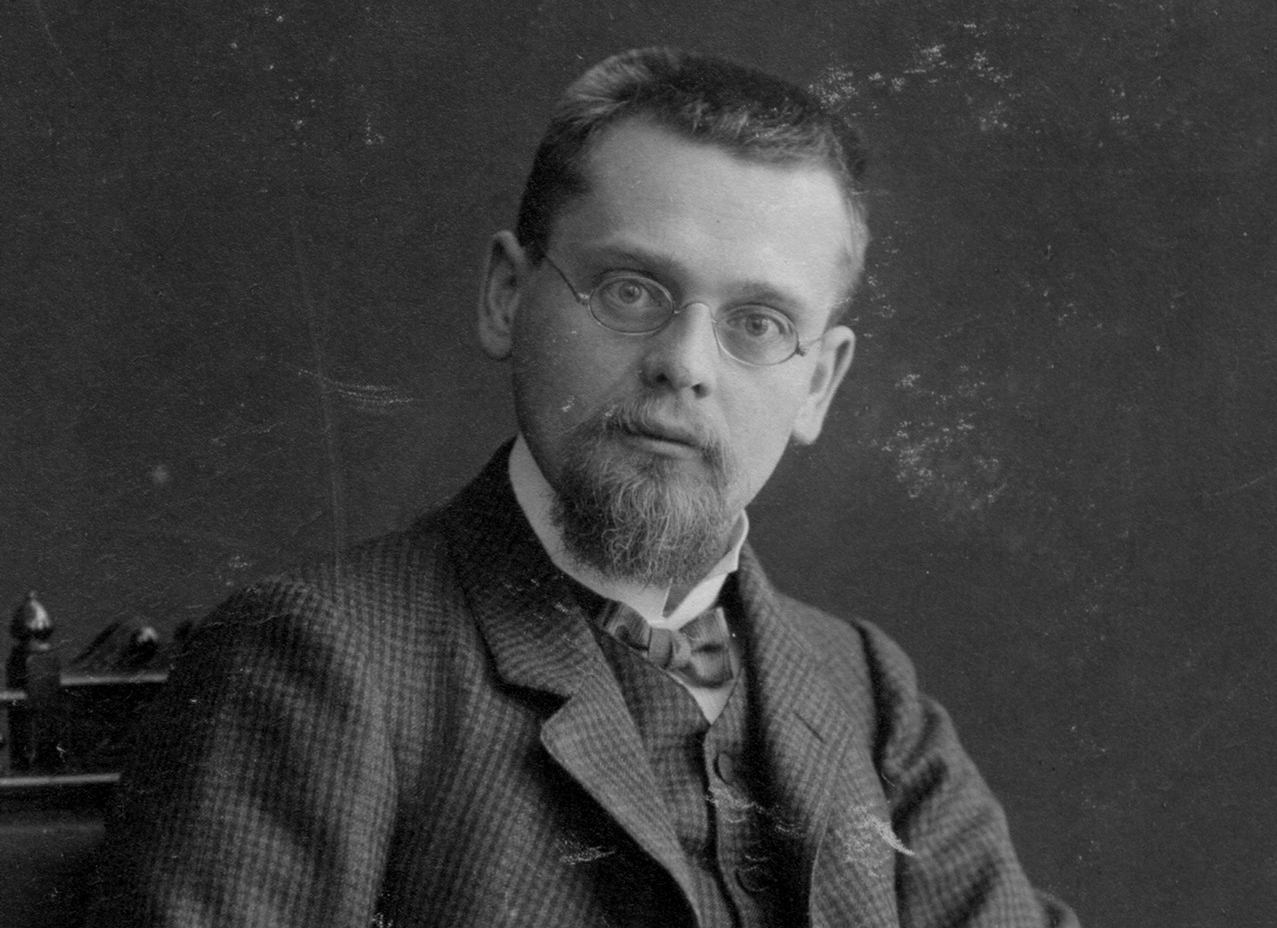
\includegraphics[width=13.5cm]{../resources/jpg/2.2.set.operations/zermelo.jpg}
    \caption*{Ernst Zermelo.}
\end{figure}
\subsection[Outermost sets in a difference is a superset.]
    {
        \color{section}Theorem 42 \color{black} : Outer sets of a difference is a superset.
    }
\documentclass[preview]{standalone}
\usepackage{amssymb, amsthm}
\usepackage{mathtools}
\usepackage{bm}


\newtheorem{theorem}{Theorem}
\renewcommand\qedsymbol{$\blacksquare$}


\begin{document}


\begin{theorem}[\textbf{2218c}]
    Let \bm{$\mathrm{A}$}, \bm{$\Lambda$}, and \bm{$\Delta$} be sets. 
    \bm{$
    \big \langle \mathrm{A} - \Lambda \big \rangle - \Delta 
        \subseteq 
    \big \langle \mathrm{A} - \Delta \big \rangle
    $}.
\end{theorem}
\begin{proof}
    Let \bm{$\lambda$} be an element in 
    \bm{$\big \langle \mathrm{A} - \Lambda \big \rangle - \Delta$}. 
    By the definition for set difference, that is
    \begin{equation*}
        \bigg[
            \Big \langle \lambda \in \mathrm{A} \Big \rangle
                \land
            \Big \langle \lambda \notin \Lambda \Big \rangle
        \bigg]
            \land
        \Big \langle \lambda \notin \Delta \Big \rangle
    \end{equation*}
    By the law of associativity for logical conjunction, 
    by the law of commutativity for logical conjunction,
    and by the simplification rule of inference,
    \begin{equation*}
        \Bigg\{
            \bigg[
                \Big \langle \lambda \in \mathrm{A} \Big \rangle
                    \land
                \Big \langle \lambda \notin \Lambda \Big \rangle
            \bigg]
                \land
            \Big \langle \lambda \notin \Delta \Big \rangle
        \Bigg\}
            \equiv
        \Bigg\{
            \bigg[
                \Big \langle \lambda \in \mathrm{A} \Big \rangle
                    \land
                \Big \langle \lambda \notin \Delta \Big \rangle
            \bigg]
                \land
            \Big \langle \lambda \notin \Lambda \Big \rangle
        \Bigg\}
    \end{equation*}
    \begin{equation*}
            \to
        \Big \langle \lambda \in \mathrm{A} \Big \rangle
            \land
        \Big \langle \lambda \notin \Delta \Big \rangle
    \end{equation*}
    $\therefore \text{\space} \bm{
    \big \langle \mathrm{A} - \Lambda \big \rangle - \Delta 
        \subseteq 
    \big \langle \mathrm{A} - \Delta \big \rangle
    }$,
    by the definitions for set difference and subsets.
\end{proof}


\end{document}
\pagebreak


% ============================= 0043 Theorem 2218d ===============================
\subsection[Alpha minus delta intersect delta $\dots$]
    {
        \color{section}Theorem 43 \color{black} : alpha minus delta intersect delta $\dots$
    }
\documentclass[preview]{standalone}
\usepackage{amssymb, amsthm}
\usepackage{mathtools}
\usepackage{bm}


\newtheorem{theorem}{Theorem}
\renewcommand\qedsymbol{$\blacksquare$}


\begin{document}


\begin{theorem}[\textbf{2218d}]
    Let \bm{$\mathrm{A}$}, \bm{$\Lambda$}, and \bm{$\Delta$} be sets. 
    \bm{$
    \big \langle \mathrm{A} - \Delta \big \rangle
        \cap 
    \big \langle \Delta - \Lambda \big \rangle
        = 
    \varnothing
    $}.
\end{theorem}
\begin{proof}
    Let \bm{$\lambda$} be an element in 
    \bm{$
    \big \langle \mathrm{A} - \Delta \big \rangle
        \cap 
    \big \langle \Delta - \Lambda \big \rangle
    $}.
    By the definitions for set difference, and set intersection, that is
    \begin{equation*}
        \bigg[
            \Big \langle \lambda \in \mathrm{A} \Big \rangle
                \land
            \Big \langle \lambda \notin \Delta \Big \rangle
        \bigg]
            \land
        \bigg[
            \Big \langle \lambda \in \Delta \Big \rangle
                \land
            \Big \langle \lambda \notin \Lambda \Big \rangle
        \bigg]
    \end{equation*}
    Since logical conjunction is associative, 
    \bm{$\lambda$} is in \bm{$\Delta$},
    and \bm{$\lambda$} is not in \bm{$\Delta$}. 
    Thus, by the negation law of logic,
    \begin{equation*}
        \Big \langle \lambda \in \mathrm{A} \Big \rangle
            \land
        \Big \langle \bot \Big \rangle
            \land
        \Big \langle \lambda \notin \Lambda \Big \rangle
    \end{equation*}
    This statement is \bm{$\bot$}, 
    by the domination law for logical conjunction. 
    And the logical identity for \bm{$\lambda \in \varnothing$} is trivially \bm{$\bot$},
    since the empty set contains no members. 
    Hence,
    \begin{equation*}
        \bigg[
            \Big \langle \lambda \in \mathrm{A} \Big \rangle
                \land
            \Big \langle \lambda \notin \Delta \Big \rangle
        \bigg]
            \land
        \bigg[
            \Big \langle \lambda \in \Delta \Big \rangle
                \land
            \Big \langle \lambda \notin \Lambda \Big \rangle
        \bigg]
            \equiv
        \Big \langle \lambda \in \varnothing \Big \rangle
    \end{equation*}
    $\therefore \text{\space} \bm{
    \big \langle \mathrm{A} - \Delta \big \rangle
        \cap 
    \big \langle \Delta - \Lambda \big \rangle
        = 
    \varnothing
    }$,
    by the definitions for the difference of sets, 
    and for the intersection of sets.
\end{proof}


\end{document}
\vspace{2\baselineskip}
\begin{figure}[!h]
    \centering
    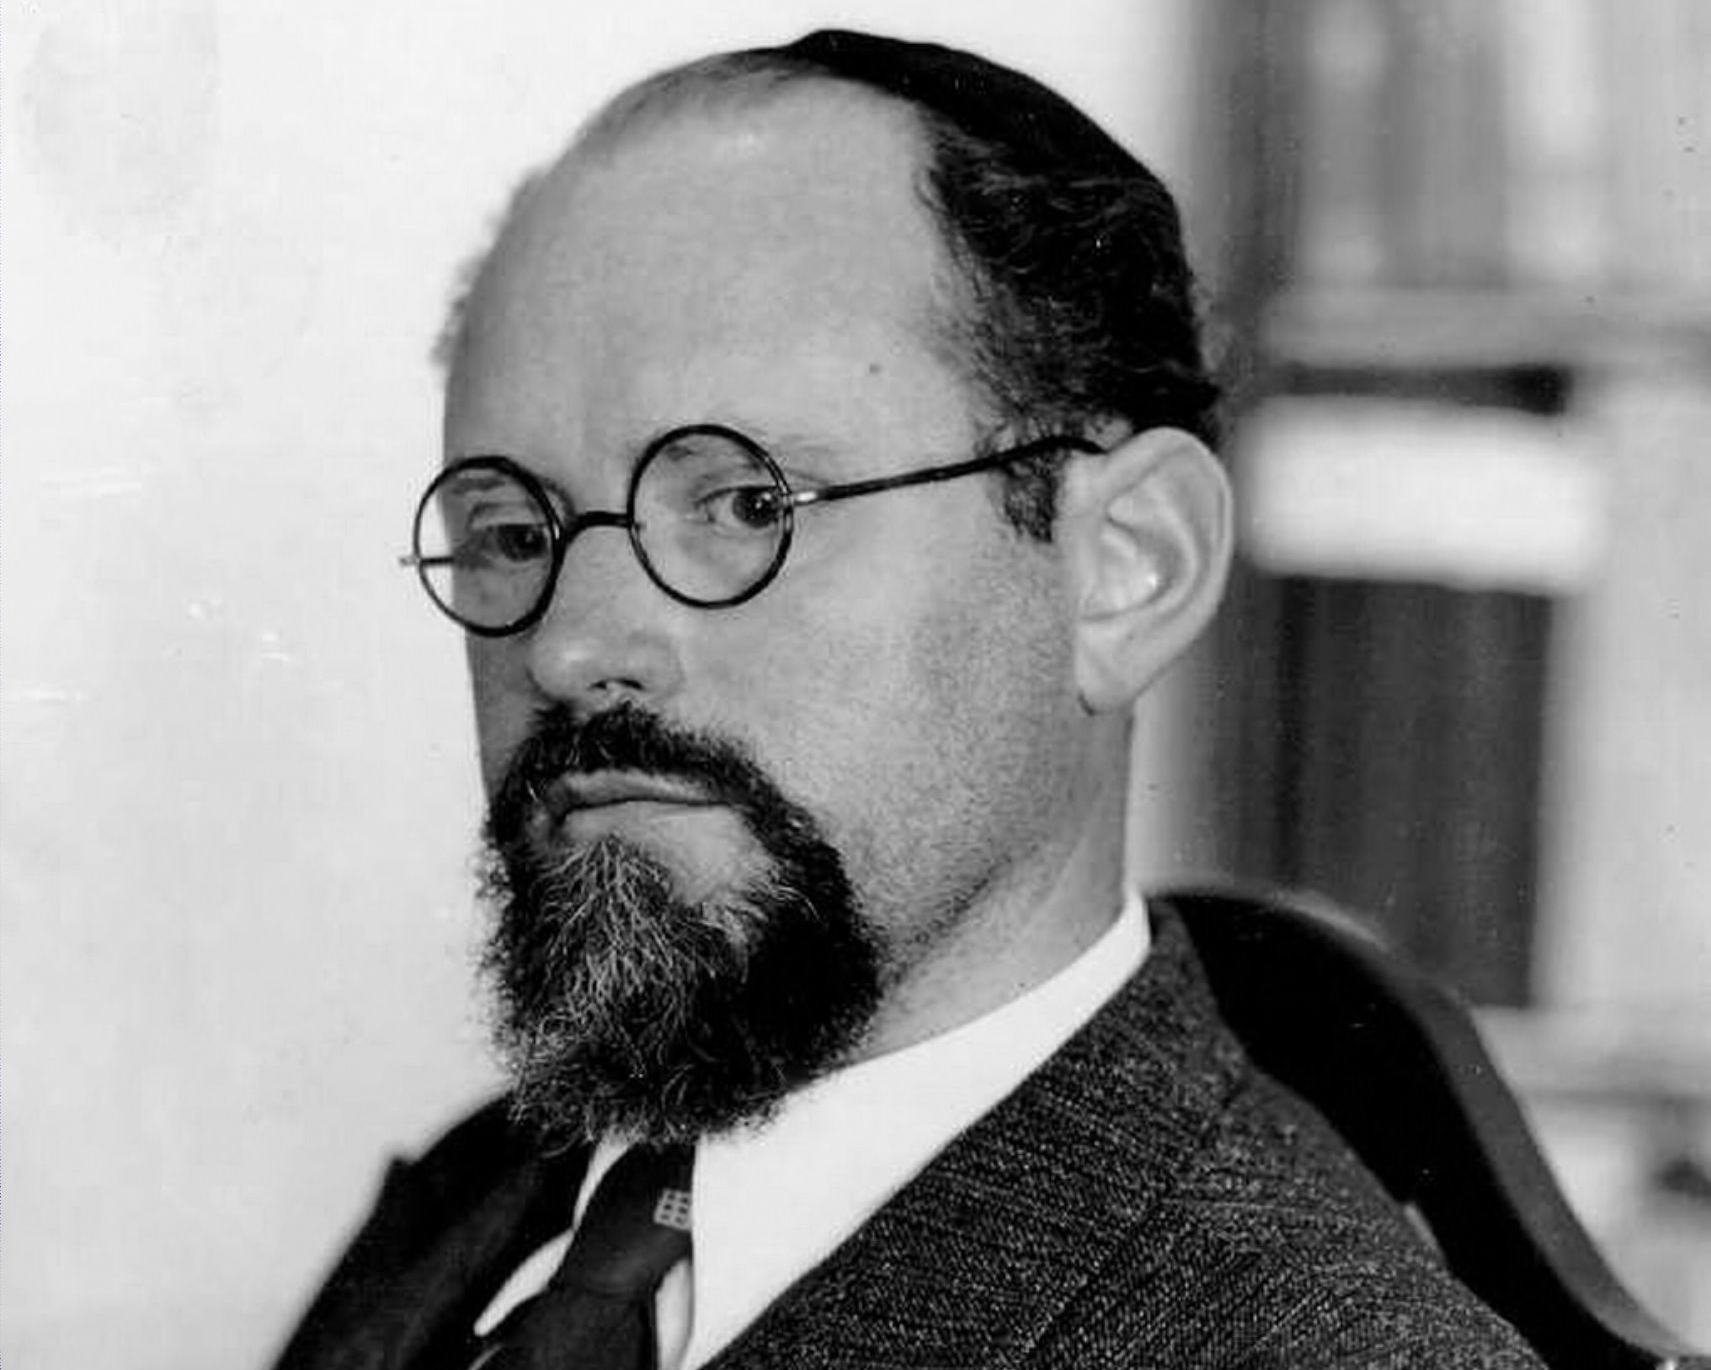
\includegraphics[width=9.5cm]{../resources/jpg/2.2.set.operations/fraenkel.jpg}
    \caption*{Abraham Fraenkel.}
\end{figure}
\pagebreak


% ============================= 0044 Theorem 2218e ===============================
\subsection[Lambda minus alpha union delta $\dots$]
    {
        \color{section}Theorem 44 \color{black} : lambda minus alpha union delta $\dots$
    }
\documentclass[preview]{standalone}
\usepackage{amssymb, amsthm}
\usepackage{mathtools}
\usepackage{bm}


\newtheorem{theorem}{Theorem}
\renewcommand\qedsymbol{$\blacksquare$}


\begin{document}


\begin{theorem}[\textbf{2218e}]
    Let \bm{$\mathrm{A}$}, \bm{$\Lambda$}, and \bm{$\Delta$} be sets. 
    \bm{$
    \big \langle \Lambda - \mathrm{A} \big \rangle 
        \cup 
    \big \langle \Delta - \mathrm{A} \big \rangle 
        = 
    \big \langle \Lambda \cup \Delta \big \rangle - \mathrm{A}
    $}.
\end{theorem}
\begin{proof} \color{black}
    Let \bm{$\lambda$} be an element in 
    \bm{$
    \big \langle \Lambda - \mathrm{A} \big \rangle 
        \cup 
    \big \langle \Delta - \mathrm{A} \big \rangle
    $}.
    By the definitions for set difference, and the union of sets, that is
    \begin{equation*}
        \bigg[
            \Big \langle \lambda \in \Lambda \Big \rangle
                \land
            \Big \langle \lambda \notin \mathrm{A} \Big \rangle
        \bigg]
            \lor
        \bigg[
            \Big \langle \lambda \in \Delta \Big \rangle
                \land
            \Big \langle \lambda \notin \mathrm{A} \Big \rangle
        \bigg]
    \end{equation*}
    Factoring \bm{$\lambda \notin \mathrm{A}$} out, 
    by the distributive laws for logical conjunction over disjunction,
    \begin{equation*}
        \Bigg\{
            \bigg[
                \Big \langle \lambda \in \Lambda \Big \rangle
                    \land
                \Big \langle \lambda \notin \mathrm{A} \Big \rangle
            \bigg]
                \lor
            \bigg[
                \Big \langle \lambda \in \Delta \Big \rangle
                    \land
                \Big \langle \lambda \notin \mathrm{A} \Big \rangle
            \bigg]
        \Bigg\}
            \equiv
    \end{equation*}
    \begin{equation*}
        \Bigg\{
            \bigg[
                \Big \langle \lambda \in \Lambda \Big \rangle
                    \lor
                \Big \langle \lambda \in \Delta \Big \rangle
            \bigg]
                \land
            \Big \langle \lambda \notin \mathrm{A} \Big \rangle
        \Bigg\}
    \end{equation*}
    $\therefore \text{\space} \bm{
    \big \langle \Lambda - \mathrm{A} \big \rangle 
        \cup 
    \big \langle \Delta - \mathrm{A} \big \rangle 
        = 
    \big \langle \Lambda \cup \Delta \big \rangle - \mathrm{A}
    }$,
    by the defintions for set difference, and set union.
\end{proof}


\end{document}
\sep
\vspace{0.5\baselineskip}


% ============================= 0045 Theorem 2219 ================================
\subsection[Alpha intersect complement lambda.]
    {
        \color{section}Theorem 45 \color{black} : alpha intersect complement lambda.
    }
\documentclass[preview]{standalone}
\usepackage{amssymb, amsthm}
\usepackage{mathtools}
\usepackage{bm}


\newtheorem{theorem}{Theorem}
\renewcommand\qedsymbol{$\blacksquare$}


\begin{document}


\begin{theorem}[\textbf{2219}]
    Let \bm{$\mathrm{A}$}, and \bm{$\Lambda$} be sets. 
    \bm{$
    \mathrm{A} - \Lambda 
        = 
    \mathrm{A} \cap \overline{\Lambda}
    $}.
\end{theorem}
\begin{proof}
    Let \bm{$\lambda$} be an element in \bm{$\mathrm{A} - \Lambda$}. 
    By the definition for set difference,
    \begin{equation*}
        \Big \langle \lambda \in \mathrm{A} \Big \rangle
            \land
        \Big \langle \lambda \notin \Lambda \Big \rangle
    \end{equation*}
    By the definition for set complementation,
    \begin{equation*}
        \bigg[
            \Big \langle \lambda \in \mathrm{A} \Big \rangle
                \land
            \Big \langle \lambda \notin \Lambda \Big \rangle
        \bigg]
            \equiv
        \bigg[
            \Big \langle \lambda \in \mathrm{A} \Big \rangle
                \land
            \Big \langle \lambda \in \overline{\Lambda} \Big \rangle
        \bigg]
    \end{equation*}
    $\therefore \text{\space} \bm{
    \mathrm{A} - \Lambda 
        = 
    \mathrm{A} \cap \overline{\Lambda}
    }$,
    by the definition for the intersection of sets.
\end{proof}


\end{document}
\pagebreak


% ============================= 0046 Theorem 2220 ================================
\subsection[An identity for the set alpha.]
    {
        \color{section}Theorem 46 \color{black} : an identity for the set alpha.
    }
\documentclass[preview]{standalone}
\usepackage{amssymb, amsthm}
\usepackage{mathtools}
\usepackage{bm}


\newtheorem{theorem}{Theorem}
\renewcommand\qedsymbol{$\blacksquare$}


\begin{document}


\begin{theorem}[\textbf{2220}]
    Let \bm{$\mathrm{A}$}, and \bm{$\Lambda$} be sets. 
    \bm{$
    \big \langle \mathrm{A} \cap \Lambda \big \rangle 
        \cup 
    \big \langle \mathrm{A} \cap \overline{\Lambda} \big \rangle 
        = 
    \mathrm{A}
    $}.
\end{theorem}
\begin{proof}
    Let \bm{$\lambda$} be an element in 
    \bm{$
    \big \langle \mathrm{A} \cap \Lambda \big \rangle 
        \cup 
    \big \langle \mathrm{A} \cap \overline{\Lambda} \big \rangle
    $}.
    By the definitions for the union of sets, and set intersection, that is,
    \begin{equation*}
        \bigg[
            \Big \langle \lambda \in \mathrm{A} \Big \rangle
                \land
            \Big \langle \lambda \in \Lambda \Big \rangle
        \bigg]
            \lor
        \bigg[
            \Big \langle \lambda \in \mathrm{A} \Big \rangle
                \land
            \Big \langle \lambda \in \overline{\Lambda} \Big \rangle
        \bigg]
    \end{equation*} 
    By the law of distribution for logical conjunction over disjunction,
    we can factor out the term \bm{$\lambda \in \mathrm{A}$}. 
    Hence, the following statement is equivalent,
    \begin{equation*}
        \Big \langle \lambda \in \mathrm{A} \Big \rangle
            \land
        \bigg[
            \Big \langle \lambda \in \Lambda \Big \rangle
                \lor
            \Big \langle \lambda \in \overline{\Lambda} \Big \rangle
        \bigg]
    \end{equation*}
    \bm{$
    \lambda \in \Lambda 
        \lor 
    \lambda \in \overline{\Lambda} 
        \equiv 
    \top
    $},
    by the negation laws of logic.
    Thus, by the identity law for logical conjunction,
    \begin{equation*}
        \Bigg\{
            \bigg[
                \Big \langle \lambda \in \mathrm{A} \Big \rangle
                    \land
                \Big \langle \lambda \in \Lambda \Big \rangle
            \bigg]
                \lor
            \bigg[
                \Big \langle \lambda \in \mathrm{A} \Big \rangle
                    \land
                \Big \langle \lambda \in \overline{\Lambda} \Big \rangle
            \bigg]
        \Bigg\}
            \equiv
        \Bigg\{
            \Big \langle \lambda \in \mathrm{A} \Big \rangle
                \land
            \Big \langle \top \Big \rangle
        \Bigg\}
            \equiv
    \end{equation*}
    \begin{equation*}
        \Big \langle \lambda \in \mathrm{A} \Big \rangle
    \end{equation*}
    $
    \therefore \text{\space} \bm{
    \big \langle \mathrm{A} \cap \Lambda \big \rangle 
        \cup 
    \big \langle \mathrm{A} \cap \overline{\Lambda} \big \rangle
        = 
    \mathrm{A}
    }$.
\end{proof}


\end{document}
\sep


% ============================= 0047 Theorem 2221 ================================
\subsection[The associative law for set union.]
    {
        \color{section}Theorem 47 \color{black} : the associative law for set union.
    }
\documentclass[preview]{standalone}
\usepackage{amssymb, amsthm}
\usepackage{mathtools}
\usepackage{bm}


\newtheorem{theorem}{Theorem}
\renewcommand\qedsymbol{$\blacksquare$}


\begin{document}


\begin{theorem}[\textbf{2221}]
    Let \bm{$\mathrm{A}$}, \bm{$\Lambda$}, and \bm{$\Delta$} be sets. 
    Set union is associative such that
    \begin{equation*}
        \bm{
            \mathrm{A} 
                \cup 
            \big \langle \Lambda \cup \Delta \big \rangle 
                = 
            \big \langle \mathrm{A} \cup \Lambda \big \rangle 
                \cup 
            \Delta
        } 
    \end{equation*}
\end{theorem}
\begin{proof}
    Let \bm{$\lambda$} be an element in 
    \bm{$
    \mathrm{A} 
        \cup 
    \big \langle \Lambda \cup \Delta \big \rangle
    $}. 
    By the definition for the union of sets, that is
    \begin{equation*}
        \Big \langle \lambda \in \mathrm{A} \Big \rangle
            \lor
        \bigg[
            \Big \langle \lambda \in \Lambda \Big \rangle
                \lor
            \Big \langle \lambda \in \Delta \Big \rangle
        \bigg]
    \end{equation*}
    It trivially follows from the associative law for logical disjunction that
    \begin{equation*}
        \Big \langle \lambda \in \mathrm{A} \Big \rangle
            \lor
        \bigg[
            \Big \langle \lambda \in \Lambda \Big \rangle
                \lor
            \Big \langle \lambda \in \Delta \Big \rangle
        \bigg]
            \equiv
        \bigg[
            \Big \langle \lambda \in \mathrm{A} \Big \rangle
                \lor
            \Big \langle \lambda \in \Lambda \Big \rangle
        \bigg]
            \lor
        \Big \langle \lambda \in \Delta \Big \rangle
    \end{equation*}
    $\therefore \text{\space} \bm{
    \mathrm{A} 
        \cup 
    \big \langle \Lambda \cup \Delta \big \rangle 
        = 
    \big \langle \mathrm{A} \cup \Lambda \big \rangle 
        \cup 
    \Delta
    }$, 
    such that set union is associative.
    by the definition for the union of sets.
\end{proof}


\end{document}
\pagebreak


% ============================= 0048 Theorem 2222 ================================
\subsection[The associative law for set intersection.]
    {
        \color{section}Theorem 48 \color{black} : the associative law for set intersection.
    }
\documentclass[preview]{standalone}
\usepackage{amssymb, amsthm}
\usepackage{mathtools}
\usepackage{bm}


\newtheorem{theorem}{Theorem}
\renewcommand\qedsymbol{$\blacksquare$}


\begin{document}


\begin{theorem}[\textbf{2222}]
    Let \bm{$\mathrm{A}$}, \bm{$\Lambda$}, and \bm{$\Delta$} be sets. 
    Set intersection is associative such that
    \begin{equation*}
        \bm{
            \mathrm{A} 
                \cap 
            \big \langle \Lambda \cap \Delta \big \rangle 
                = 
            \big \langle \mathrm{A} \cap \Lambda \big \rangle
                \cap 
            \Delta
        }
\end{equation*}
\end{theorem}
\begin{proof}
    Let \bm{$\lambda$} be an element in 
    \bm{$
    \mathrm{A} 
        \cap 
    \big \langle \Lambda \cap \Delta \big \rangle
    $}. 
    By the definition for the intersection of sets, that is 
    \begin{equation*}
        \Big \langle \lambda \in \mathrm{A} \Big \rangle
            \land
        \bigg[
            \Big \langle \lambda \in \Lambda \Big \rangle
                \land
            \Big \langle \lambda \in \Delta \Big \rangle
        \bigg]
    \end{equation*}
    It trivially follows from the associative law for logical conjunction that
    \begin{equation*}
        \Big \langle \lambda \in \mathrm{A} \Big \rangle
            \land
        \bigg[
            \Big \langle \lambda \in \Lambda \Big \rangle
                \land
            \Big \langle \lambda \in \Delta \Big \rangle
        \bigg]
            \equiv
        \bigg[
            \Big \langle \lambda \in \mathrm{A} \Big \rangle
                \land
            \Big \langle \lambda \in \Lambda \Big \rangle
        \bigg]
            \land
        \Big \langle \lambda \in \Delta \Big \rangle
    \end{equation*}
    $
    \therefore \text{\space} \bm{
    \mathrm{A} 
        \cap 
    \big \langle \Lambda \cap \Delta \big \rangle 
        = 
    \big \langle \mathrm{A} \cap \Lambda \big \rangle
        \cap 
    \Delta
    }$,
    such that set intersection is associative,
    by the definition for the intersection of sets.
\end{proof}


\end{document}
\vspace{2.5\baselineskip}
\begin{figure}[!h]
    \centering
    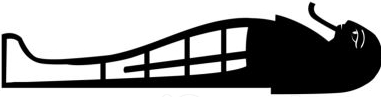
\includegraphics[width=7cm]{../resources/jpg/2.2.set.operations/border7.jpg}
\end{figure}
\vspace{2\baselineskip}


% ============================= 0049 Theorem 2223 ================================
\subsection[Union is distributive over intersection.]
    {
        \color{section}Theorem 49 \color{black} : union is distributive over intersection.
    }
\documentclass[preview]{standalone}
\usepackage{amssymb, amsthm}
\usepackage{mathtools}
\usepackage{bm}


\newtheorem{theorem}{Theorem}
\renewcommand\qedsymbol{$\blacksquare$}


\begin{document}


\begin{theorem}[\textbf{2223}]
    Let \bm{$\mathrm{A}$}, \bm{$\Lambda$}, and \bm{$\Delta$} be sets.
    Set union is distributive over set intersection such that
    \begin{equation*}
        \bm{
            \mathrm{A} \cup \Big \langle \Lambda \cap \Delta \Big \rangle 
                =
            \Big \langle \mathrm{A} \cup \Lambda \Big \rangle
                \cap 
            \Big \langle \mathrm{A} \cup \Delta \Big \rangle
        }
    \end{equation*}
\end{theorem}
\begin{proof}
    Let \bm{$\lambda$} be an element in 
    \bm{$
    \mathrm{A} \cup \big \langle \Lambda \cap \Delta \big \rangle
    $}.
    By the defintions for the union and intersection of sets, that is 
    \begin{equation*}
        \big \langle \lambda \in \mathrm{A} \big \rangle
            \lor
        \Big[
            \big \langle \lambda \in \Lambda \big \rangle
                \land
            \big \langle \lambda \in \Delta \big \rangle
        \Big]
    \end{equation*}
    By the law of distribution for logical disjunction over conjunction,
    \begin{equation*}
        \big \langle \lambda \in \mathrm{A} \big \rangle
            \lor
        \Big[
            \big \langle \lambda \in \Lambda \big \rangle
                \land
            \big \langle \lambda \in \Delta \big \rangle
        \Big] 
            \equiv
        \Big[
            \big \langle \lambda \in \mathrm{A} \big \rangle
                \lor
            \big \langle \lambda \in \Lambda \big \rangle
        \Big]
            \land
        \Big[
            \big \langle \lambda \in \mathrm{A} \big \rangle
                \lor
            \big \langle \lambda \in \Delta \big \rangle
        \Big]
    \end{equation*}
    $\therefore \text{\space} \bm{
    \mathrm{A} \cup \big \langle \Lambda \cap \Delta \big \rangle 
        = 
    \big \langle \mathrm{A} \cup \Lambda \big \rangle
        \cap 
    \big \langle \mathrm{A} \cup \Delta \big \rangle
    }$, 
    such that set union is distributive over set intersection,
    by the definitons for set union and set intersection.
\end{proof}


\end{document}
\pagebreak


% ============================= 0050 Theorem 2224 ================================
\subsection[The distribution of differences.]
    {
        \color{section}Theorem 50 \color{black} : the distribution of differences.
    }
\documentclass[preview]{standalone}
\usepackage{amssymb, amsthm}
\usepackage{mathtools}
\usepackage{bm}


\newtheorem{theorem}{Theorem}
\renewcommand\qedsymbol{$\blacksquare$}


\begin{document}


\begin{theorem}[\textbf{2224}]
    Let \bm{$\mathrm{A}$}, \bm{$\Lambda$}, and \bm{$\Delta$} be sets. 
    \begin{equation*}
        \bm{
            \Big \langle \mathrm{A} - \Lambda \Big \rangle - \Delta 
                = 
            \Big \langle \mathrm{A} - \Delta \Big \rangle 
                - 
            \Big \langle \Lambda - \Delta \Big \rangle
        }
    \end{equation*}
\end{theorem}
\begin{proof}
    Let \bm{$\lambda$} be an element in 
    \bm{$
    \big \langle \mathrm{A} - \Lambda \big \rangle - \Delta 
    $}. 
    By the definition for set difference,
    \begin{equation*}
        \bigg[
            \Big \langle \lambda \in \mathrm{A} \Big \rangle
                \land
            \Big \langle \lambda \notin \Lambda \Big \rangle
        \bigg]
            \land
        \Big \langle \lambda \notin \Delta \Big \rangle
    \end{equation*}
    Note that, by the indentity law for logical disjunction, 
    \bm{$
    \lambda \notin \Lambda
        \equiv 
    \lambda \notin \Lambda
        \lor 
    \bot
    $}.
    And since
    \bm{$
    \lambda \in \Delta
        \equiv 
    \bot
    $},
    by definition,
    it follows that
    \begin{equation*}
        \Big \langle \lambda \notin \Lambda \Big \rangle
            \equiv
        \bigg[
            \Big \langle \lambda \notin \Lambda \Big \rangle
                \lor
            \Big \langle \bot \Big \rangle
        \bigg]
            \equiv
        \bigg[
            \Big \langle \lambda \notin \Lambda \Big \rangle
                \lor
            \Big \langle \lambda \in \Delta \Big \rangle
        \bigg]
    \end{equation*}
    Moreover, by the double negation law of logic, and by DeMorgans laws,
    \begin{equation*}
        \Big \langle \lambda \notin \Lambda \Big \rangle
            \equiv
        \lnot \Bigg\{
            \lnot \bigg[
                \Big \langle \lambda \notin \Lambda \Big \rangle
                    \lor
                \Big \langle \lambda \in \Delta \Big \rangle
            \bigg]
        \Bigg\}
            \equiv
        \lnot \bigg[
            \Big \langle \lambda \in \Lambda \Big \rangle
                \land
            \Big \langle \lambda \notin \Delta \Big \rangle
        \bigg]
    \end{equation*}
    Thus, the proposition
    \bm{$
    \lambda \in
    \big \langle \mathrm{A} - \Lambda \big \rangle - \Delta 
    $},
    is equivalent to
    \begin{equation*}
        \Bigg\{
        \Big \langle \lambda \in \mathrm{A} \Big \rangle
            \land
        \lnot \bigg[
            \Big \langle \lambda \in \Lambda \Big \rangle
                \land
            \Big \langle \lambda \notin \Delta \Big \rangle
        \bigg]
        \Bigg\}
            \land
        \Big \langle \lambda \notin \Delta \Big \rangle
    \end{equation*}
    By law of commutativity (and association) for logical conjunction, 
    that is
    \begin{equation*}
        \bigg[
            \Big \langle \lambda \in \mathrm{A} \Big \rangle
                \land
            \Big \langle \lambda \notin \Delta \Big \rangle
        \bigg]
            \land
        \lnot \bigg[
            \Big \langle \lambda \in \Lambda \Big \rangle
                \land
            \Big \langle \lambda \notin \Delta \Big \rangle
        \bigg]
    \end{equation*}
    By the definitions for the difference of sets, set complementation,
    and the intersection of sets,
    \begin{equation*}
        \bigg[
        \Big \langle \mathrm{A} - \Lambda \Big \rangle - \Delta
        \bigg]
            \equiv
        \bigg[
        \Big \langle \mathrm{A} - \Delta \Big \rangle
            \cap
        \overline{
            \Big \langle \Lambda - \Delta \Big \rangle
        }
        \bigg]
    \end{equation*}
    $\therefore \text{\space} \bm{
    \big \langle \mathrm{A} - \Lambda \big \rangle - \Delta 
        = 
    \big \langle \mathrm{A} - \Delta \big \rangle 
        - 
    \big \langle \Lambda - \Delta \big \rangle
    }$, by Thereom 45.

\end{proof}


\end{document}
\sep
\pagebreak


% ============================= 0051 Theorem 2231 ================================
\subsection[Subsets are contrapositive.]
    {
        \color{section}Theorem 51 \color{black} : Subsets are contrapositive.
    }
\documentclass[preview]{standalone}
\usepackage{amssymb, amsthm}
\usepackage{mathtools}
\usepackage{bm}


\newtheorem{theorem}{Theorem}
\renewcommand\qedsymbol{$\blacksquare$}


\begin{document}


\begin{theorem}[\textbf{2231}]
    Let \bm{$\mathrm{A}$}, and \bm{$\Lambda$} be subsets of a universal set \bm{$\Omega$}. 
    \begin{equation*}
        \bm{
            \mathrm{A} \subseteq \Lambda
                \text{ if and only if } 
            \overline{\Lambda} \subseteq \overline{\mathrm{A}}
            }
    \end{equation*}
\end{theorem}
\begin{proof}
    The proposition \bm{$\mathrm{A} \subseteq \Lambda$} is defined by the universal quantification% statement 
    \begin{equation*}
        \forall \lambda \Big \langle \lambda \in \mathrm{A} \rightarrow \lambda \in \Lambda \Big \rangle
    \end{equation*}
    Where \bm{$\lambda$} is an element in the domain of discourse \bm{$\Omega$}.
    It is a tautology that the truth value for the predicate is equivalent to its contrapositive. 
    Thus,  
    \begin{equation*}
        \forall \lambda \Big \langle \lambda \notin \Lambda \rightarrow \lambda \notin \mathrm{A} \Big \rangle
    \end{equation*} 
    By the definition for set complementation, and subsets
    \bm{$\lambda \in \overline{\Lambda} \subseteq \overline{\mathrm{A}}$} 
    $\therefore$ \bm{$\mathrm{A} \subseteq \Lambda$} \textbf{\emph{ iff }} \bm{$\overline{\Lambda} \subseteq \overline{\mathrm{A}}$}.
\end{proof}


\end{document}
\vspace{2.5\baselineskip}
\begin{figure}[!h]
    \centering
    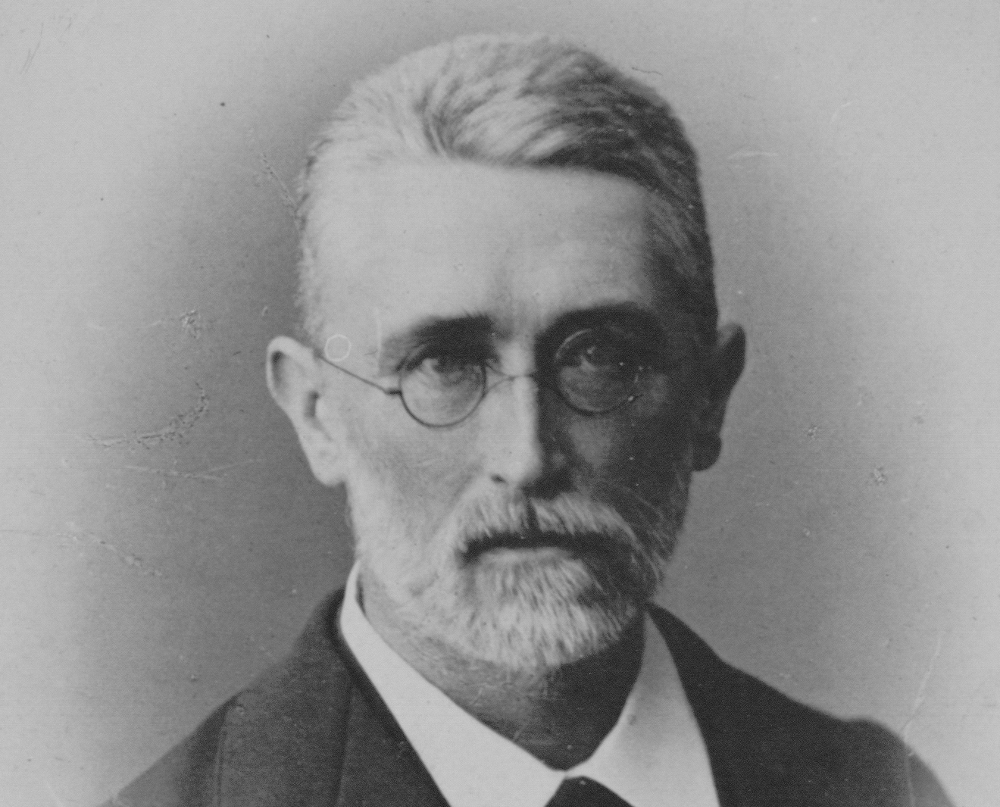
\includegraphics[width=13cm]{../resources/jpg/2.2.set.operations/dedekind.png}
    \caption*{Richard Dedekind.}
\end{figure}
\pagebreak


% ============================= 0052 Theorem 2235 ================================
\subsection[Symmetric difference is a set difference.]
    {
        \color{section}Theorem 52 \color{black} : symmetric difference is a set difference.
    }
\documentclass[preview]{standalone}
\usepackage{amssymb, amsthm}
\usepackage{mathtools}
\usepackage{bm}


\newtheorem{theorem}{Theorem}
\renewcommand\qedsymbol{$\blacksquare$}


\begin{document}


\begin{theorem}[\textbf{2235}]
    Let \bm{$\mathrm{A}$}, and \bm{$\Lambda$} be sets. 
    \bm{$
    \mathrm{A} \oplus \Lambda 
        = 
    \big \langle \mathrm{A} \cup \Lambda \big \rangle 
        - 
    \big \langle \mathrm{A} \cap \Lambda \big \rangle
    $}.
\end{theorem}
\begin{proof}
    Let \bm{$\lambda$} be an element in \bm{$\mathrm{A} \oplus \Lambda$}. 
    By the definition for the symmetric difference of sets,
    \begin{equation*}
        \bigg[
            \Big \langle \lambda \in \mathrm{A} \Big \rangle 
                \land 
            \Big \langle \lambda \notin \Lambda \Big \rangle
        \bigg] 
            \lor 
        \bigg[
            \Big \langle \lambda \notin \mathrm{A} \Big \rangle
                \land 
            \Big \langle \lambda \in \Lambda \Big \rangle
        \bigg]
    \end{equation*}
    Distributing the right-hand side over the left-hand side,
    by the distributive laws of logic, that is
    \begin{equation*}
        \Bigg\{
            \Big \langle \lambda \in \mathrm{A} \Big \rangle
                \lor
            \bigg[
                \Big \langle \lambda \notin \mathrm{A} \Big \rangle
                    \land 
                \Big \langle \lambda \in \Lambda \Big \rangle
            \bigg]
        \Bigg\}
            \land
        \Bigg\{
            \Big \langle \lambda \notin \Lambda \Big \rangle
                \lor
            \bigg[
                \Big \langle \lambda \notin \mathrm{A} \Big \rangle
                    \land 
                \Big \langle \lambda \in \Lambda \Big \rangle
            \bigg]
        \Bigg\}
    \end{equation*}
    Again, by the distributive law for logical disjunction over conjunction,
    and by the associative law for logical conjunction, we have
    \begin{equation*}
        \bigg[
            \Big \langle \lambda \in \mathrm{A} \Big \rangle
                \lor
            \Big \langle \lambda \notin \mathrm{A} \Big \rangle
        \bigg]
            \land
        \bigg[
            \Big \langle \lambda \in \mathrm{A} \Big \rangle
                \lor 
            \Big \langle \lambda \in \Lambda \Big \rangle
        \bigg]
            \land
        \bigg[
            \Big \langle \lambda \notin \Lambda \Big \rangle
                \lor
            \Big \langle \lambda \notin \mathrm{A} \Big \rangle
        \bigg]
            \land
    \end{equation*}
    \begin{equation*}
        \bigg[
            \Big \langle \lambda \notin \Lambda \Big \rangle
                \lor 
            \Big \langle \lambda \in \Lambda \Big \rangle
        \bigg]
    \end{equation*}
    The following identity is given by the negation laws of logic,
    \begin{equation*}
        \big \langle \top \big \rangle
            \land
        \bigg[
            \Big \langle \lambda \in \mathrm{A} \Big \rangle
                \lor 
            \Big \langle \lambda \in \Lambda \Big \rangle
        \bigg]
            \land
        \bigg[
            \Big \langle \lambda \notin \Lambda \Big \rangle
                \lor
            \Big \langle \lambda \notin \mathrm{A} \Big \rangle
        \bigg]
            \land
        \big \langle \top \big \rangle
    \end{equation*}
    By DeMorgans laws,
    and by the identity law for logical conjunction, 
    that is
    \begin{equation*}
        \bigg[
            \Big \langle \lambda \in \mathrm{A} \Big \rangle
                \lor 
            \Big \langle \lambda \in \Lambda \Big \rangle
        \bigg]
            \land
        \lnot \bigg[
            \Big \langle \lambda \in \Lambda \Big \rangle
                \land
            \Big \langle \lambda \in \mathrm{A} \Big \rangle
        \bigg]
    \end{equation*}
    Which, by the definitions for set union, set intersection,
    and set membership, is equivalent to
    \begin{equation*}
        \Bigg\{
            \lambda \in \Big \langle \mathrm{A} \cup \Lambda \Big \rangle
                \land
            \lnot \bigg[ 
                \lambda \in \Big \langle \Lambda \cap \mathrm{A} \Big \rangle
            \bigg]
        \Bigg\}
            \equiv
        \Bigg\{
            \lambda \in \Big \langle \mathrm{A} \cup \Lambda \Big \rangle
                \land
            \lambda \notin \Big \langle \Lambda \cap \mathrm{A} \Big \rangle
        \Bigg\}
    \end{equation*}
    $\therefore$ by the definition for set difference,
    \bm{$
    \mathrm{A} \oplus \Lambda 
        = 
    \big \langle \mathrm{A} \cup \Lambda \big \rangle 
        - 
    \big \langle \mathrm{A} \cap \Lambda \big \rangle
    $}.
\end{proof}


\end{document}
\sep
\pagebreak


% ============================= 0053 Theorem 2236 ================================
\subsection[Symmetric difference is a union.]
    {
        \color{section}Theorem 53 \color{black} : symmetric difference is a union.
    }
\documentclass[preview]{standalone}
\usepackage{amssymb, amsthm}
\usepackage{mathtools}
\usepackage{bm}


\newtheorem{theorem}{Theorem}
\renewcommand\qedsymbol{$\blacksquare$}


\begin{document}


\begin{theorem}[\textbf{2236}]
    Let \bm{$\Gamma$}, and \bm{$\Xi$} be sets. 
    \begin{equation*}
        \bm{
            \Gamma \oplus \Xi 
                = 
            \Big \langle \Gamma - \Xi \Big \rangle
                \cup 
            \Big \langle \Xi - \Gamma \Big \rangle
        }
    \end{equation*}
\end{theorem}
\begin{proof}
    Suppose there exists an element \bm{$\zeta$} such that \bm{$\zeta$} is a member of \bm{$\Gamma \oplus \Xi$}. 
    By the definition for symmetric difference,
    \begin{equation*}
        \bigg[
            \Big \langle \zeta \in \Gamma \Big \rangle 
                \land 
            \Big \langle \zeta \notin \Xi \Big \rangle
        \bigg] 
            \lor 
        \bigg[
            \Big \langle \zeta \notin \Gamma \Big \rangle
                \land 
            \Big \langle \zeta \in \Xi \Big \rangle
        \bigg]   
    \end{equation*}
    Because logical conjunction is associative, this statement is equivalent to 
    \begin{equation*}
        \bigg[
            \Big \langle \zeta \in \Gamma \Big \rangle 
                \land 
            \Big \langle \zeta \notin \Xi \Big \rangle
        \bigg] 
            \lor 
        \bigg[
            \Big \langle \zeta \in \Xi \Big \rangle
                \land 
            \Big \langle \zeta \notin \Gamma \Big \rangle
        \bigg]   
    \end{equation*}
    $\therefore \text{\space} \bm{
        \Gamma \oplus \Xi 
        = 
    \big \langle \Gamma - \Xi \big \rangle
        \cup 
    \big \langle \Xi - \Gamma \big \rangle
    }$, by the defintions for set union and the difference of sets.
\end{proof}


\end{document}
\sep


% ============================= 0054 Theorem 2237a ===============================
\subsection[Symmetric difference between a set and itself.]
    {
        \color{section}Theorem 54 \color{black} : symmetric difference of a set itself.
    }
\documentclass[preview]{standalone}
\usepackage{amssymb, amsthm}
\usepackage{mathtools}
\usepackage{bm}


\newtheorem{theorem}{Theorem}
\renewcommand\qedsymbol{$\blacksquare$}


\begin{document}


\begin{theorem}[\textbf{2237a}]
    Let \bm{$\Gamma$} be a subset of the universal set \bm{$\Omega$}. 
    \begin{equation*}
        \bm{\Gamma \oplus \Gamma = \varnothing}
    \end{equation*}
\end{theorem}
\begin{proof}
    By Theorem 52, 
    \bm{$
    \Gamma \oplus \Gamma 
        = 
    \big \langle \Gamma \cup \Gamma \big \rangle
        - 
    \big \langle \Gamma \cap \Gamma \big \rangle
    $}. 
    By the set idempotent laws, 
    that is \bm{$\Gamma - \Gamma$}, 
    and by Theorem 45, equivalent to 
    \bm{$\Gamma \cap \overline{\Gamma}$}. 
    It follows immediately from the set complement law for the intersection of sets that 
    \bm{$\Gamma \oplus \Gamma = \varnothing$}.
\end{proof}


\end{document}
\sep


% ============================= 0055 Theorem 2237b ===============================
\subsection[Symmetric difference with the empty set.]
    {
        \color{section}Theorem 55 \color{black} : symmetric difference with the empty set.
    }
\documentclass[preview]{standalone}
\usepackage{amssymb, amsthm}
\usepackage{mathtools}
\usepackage{bm}


\newtheorem{theorem}{Theorem}
\renewcommand\qedsymbol{$\blacksquare$}


\begin{document}


\begin{theorem}[\textbf{2237b}]
    Let \bm{$\Gamma$} be a subset of the universal set \bm{$\Omega$}. 
    \begin{equation*}
        \bm{\Gamma \oplus \varnothing = \Gamma}
    \end{equation*}
\end{theorem}
\begin{proof}
    By Theorem 52, 
    \bm{$
    \Gamma \oplus \varnothing 
        = 
    \big \langle \Gamma \cup \varnothing \big \rangle
        - 
    \big \langle \Gamma \cap \varnothing \big \rangle
    $}. 
    By the identity law for set union, 
    and by the set domination law for intersection, 
    that is \bm{$\Gamma - \varnothing$}, 
    which by Theorem 45 means 
    \bm{$\Gamma \cap \overline{\bm{\varnothing}}$}. 
    Because \bm{$\overline{\bm{\varnothing}} = \Omega$},
    \bm{$\Gamma \cap \overline{\bm{\varnothing}} \equiv \Gamma \cap \Omega}$. 
    Thus, by the set identity law for intersection, 
    \bm{$\Gamma \oplus \varnothing = \Gamma$}.
\end{proof}


\end{document}
\pagebreak


% ============================= 0056 Theorem 2237c ===============================
\subsection[Symmetric difference with the universe.]
    {
        \color{section}Theorem 56 \color{black} : symmetric difference with the universe.
    }
\documentclass[preview]{standalone}
\usepackage{amssymb, amsthm}
\usepackage{mathtools}
\usepackage{bm}


\newtheorem{theorem}{Theorem}
\renewcommand\qedsymbol{$\blacksquare$}


\begin{document}


\begin{theorem}[\textbf{2237c}]
    Let \bm{$\Gamma$} be a subset of the universal set \bm{$\Omega$}. 
    \begin{equation*}
        \bm{\Gamma \oplus \Omega = \overline{\Gamma}}
    \end{equation*}
\end{theorem}
\begin{proof}
    By Theorem 52, 
    \bm{$
    \Gamma \oplus \Omega
        = 
    \big \langle \Gamma \cup \Omega \big \rangle
        - 
    \big \langle \Gamma \cap \Omega \big \rangle
    $}. 
    By the set domination law for set union, and by the set 
    identity law for set intersection, that is \bm{$\Omega - \Gamma$}. 
    Hence, by Theorem 45, 
    \bm{$\Omega \cap \overline{\Gamma}$}.
    By the identity law for set intersection,
    \bm{$\Gamma \oplus \Omega = \overline{\Gamma}$}.
\end{proof}


\end{document}
\sep


% ============================= 0057 Theorem 2237d ===============================
\subsection[Symmetric difference with a complement.]
    {
        \color{section}Theorem 57 \color{black} : symmetric difference and a complement.
    }
\documentclass[preview]{standalone}
\usepackage{amssymb, amsthm}
\usepackage{mathtools}
\usepackage{bm}


\newtheorem{theorem}{Theorem}
\renewcommand\qedsymbol{$\blacksquare$}


\begin{document}


\begin{theorem}[\textbf{2237d}]
    Let \bm{$\Xi$} be a subset of a universal set \bm{$\Omega$}. 
    \begin{equation*}
        \bm{\Xi \oplus \overline{\Xi} = \Omega}
    \end{equation*}
\end{theorem}
\begin{proof}
    By Theorem 52, 
    \bm{$
    \Xi \oplus \overline{\Xi} 
        = 
    \big \langle \Xi \cup \overline{\Xi} \big \rangle
        - 
    \big \langle \Xi \cap \overline{\Xi} \big \rangle
    $}. 
    By the set complement laws that is \bm{$\Omega - \varnothing$}. 
    Rather, \bm{$\Omega \cap \overline{\bm{\varnothing}}$}, 
    by Theorem 45. 
    Since \bm{$\overline{\bm{\varnothing}} = \Omega$}, that is 
    \bm{$\Omega \cap \Omega$}. Which is \bm{$\Omega$}, 
    by the idempotent law for set intersection.
    Thus, \bm{$\Xi \oplus \overline{\Xi} = \Omega$}.
\end{proof}


\end{document}
\begin{figure}[!h]
    \centering
    
\includegraphics[width=3cm]{../resources/jpg/2.2.set.operations/horus.png}
\end{figure}


% ============================= 0058 Theorem 2238a ===============================
\subsection[Symmetric difference is associative.]
    {
        \color{section}Theorem 58 \color{black} : symmetric difference is associative.
    }
\documentclass[preview]{standalone}
\usepackage{amssymb, amsthm}
\usepackage{mathtools}
\usepackage{bm}


\newtheorem{theorem}{Theorem}
\renewcommand\qedsymbol{$\blacksquare$}


\begin{document}


\begin{theorem}[\textbf{2238a}]
    Let \bm{$\mathrm{A}$}, and \bm{$\Lambda$} be sets. 
    Symmetric difference of sets is associative such that 
    \begin{equation*}
        \bm{
            \big \langle \mathrm{A} \oplus \Lambda \big \rangle
                = 
            \big \langle \Lambda \oplus \mathrm{A} \big \rangle
        }
    \end{equation*}
\end{theorem}
\begin{proof}
    By Theorem 52, 
    \bm{$
    \mathrm{A} \oplus \Lambda 
        = 
    \big \langle \mathrm{A} \cup \Lambda \big \rangle
        - 
    \big \langle \mathrm{A} \cap \Lambda \big \rangle
    $}. 
    Because set union is associative, and because set intersection is associative,
    trivially 
    \bm{$
    \mathrm{A} \oplus \Lambda \equiv 
    \big \langle \Lambda \cup \mathrm{A} \big \rangle
        - 
    \big \langle \Lambda \cap \mathrm{A} \big \rangle
    $};
    by Theorem 52, 
    \bm{$\Lambda \oplus \mathrm{A}$}.
\end{proof}


\end{document}
\sep
\pagebreak


% ============================= 0059 Theorem 2238b ===============================
\subsection[An identity for gamma.]
    {
        \color{section}Theorem 59 \color{black} : an identity for gamma.
    }
\documentclass[preview]{standalone}
\usepackage{amssymb, amsthm}
\usepackage{mathtools}
\usepackage{bm}


\newtheorem{theorem}{Theorem}
\renewcommand\qedsymbol{$\blacksquare$}


\begin{document}


\begin{theorem}[\textbf{2238b}]
    Let \bm{$\Gamma$}, and \bm{$\Xi$} be sets.
    \bm{$
    \big \langle \Gamma \oplus \Xi \big \rangle
        \oplus 
    \Xi 
        = 
    \Gamma$}.
\end{theorem}
\begin{proof}
    By Theorem 52, 
    \begin{equation*}
        \Big \langle \Gamma \oplus \Xi \Big \rangle 
            \oplus 
        \Xi 
            = 
        \bigg[
            \Big \langle \Gamma \oplus \Xi \Big \rangle 
                \cup 
            \Xi
        \bigg] 
            - 
        \bigg[
            \Big \langle \Gamma \oplus \Xi \Big \rangle
                \cap 
            \Xi
        \bigg]
    \end{equation*}
    By Lemma 1, that is
    \begin{equation*}
        \Bigg\{
            \bigg[
                \Big \langle \Gamma \cup \Xi \Big \rangle
                    \cap
                \Big \langle
                    \overline{\Gamma} 
                        \cup 
                    \overline{\Xi} 
                \Big \rangle
            \bigg]
                \cup
            \Xi
        \Bigg\}
            -
        \Bigg\{
            \bigg[
                \Big \langle \Gamma \cup \Xi \Big \rangle
                    \cap
                \Big \langle
                    \overline{\Gamma} 
                        \cup 
                    \overline{\Xi} 
                \Big \rangle
            \bigg]
                \cap
            \Xi
        \Bigg\}
    \end{equation*}
    Since set intersection is associative, 
    by the associative law for the intersection of sets, 
    the identities for the terms in the difference are given immediately
    by Lemma 2, and Lemma 3. Thus, 
    \begin{equation*}
        \Big \langle \Gamma \oplus \Xi \Big \rangle 
            \oplus 
        \Xi
            =
        \Big \langle \Gamma \cup \Xi \Big \rangle
            -
        \Big \langle 
            \Xi
                \cap 
            \overline{\Gamma} 
        \Big \rangle
    \end{equation*}
    By Theorem 45, 
    by DeMorgans law for the complement of intersections, 
    and by the complementation law for sets, 
    that is
    \begin{equation*}
        \bigg[
            \Big \langle \Gamma \cup \Xi \Big \rangle
                -
            \Big \langle 
                \Xi
                    \cap 
                \overline{\Gamma} 
            \Big \rangle
        \bigg]
            \equiv
        \bigg[
            \Big \langle \Gamma \cup \Xi \Big \rangle
                \cap
            \Big \langle \overline{
                \Xi
                    \cap 
                \overline{\Gamma} 
            } \Big \rangle
        \bigg]
            \equiv
        \bigg[
            \Big \langle \Gamma \cup \Xi \Big \rangle
                \cap
            \Big \langle 
                \overline{\Xi}
                    \cup 
                \Gamma
            \Big \rangle
        \bigg]
    \end{equation*}
    \bm{$\Gamma$} can be factored out,
    by the distribution law for set union over intersection.
    \begin{equation*}
        \Big \langle \Gamma \oplus \Xi \Big \rangle
            \oplus 
        \Xi
            \equiv
        \Gamma 
            \cup
        \Big \langle \Xi \cap \overline{\Xi} \Big \rangle
    \end{equation*}
    \bm{$\Xi \cap \overline{\Xi}$} is empty, 
    by the complement law for set intersection. 
    And \bm{$\Gamma$} union the empty set is \bm{$\Gamma$},
    by the identity law for set union $\therefore \bm{
    \big \langle \Gamma \oplus \Xi \big \rangle
        \oplus 
    \Xi 
        = 
    \Gamma}$.
\end{proof}


\end{document}
\begin{figure}[!h]
    \centering
    
\includegraphics[width=9cm]{../resources/jpg/2.2.set.operations/ankh.jpg}
\end{figure}
\pagebreak


% ============================= 0060 Theorem 2240 ================================
\subsection[Symmetric difference is associative.]
    {
        \color{section}Theorem 60 \color{black} : symmetric difference is associative.
    }
\documentclass[preview]{standalone}
\usepackage{amssymb, amsthm}
\usepackage{mathtools}
\usepackage{bm}


\newtheorem{theorem}{Theorem}
\renewcommand\qedsymbol{$\blacksquare$}


\begin{document}


\begin{theorem}[\textbf{2240}]
    Let \bm{$\Gamma$}, \bm{$\Pi$}, and \bm{$\Xi$} be sets. 
    The symmetric difference for sets is associative such that 
    \begin{equation*}
        \bm{
            \Big \langle \Gamma \oplus \Pi \Big \rangle
                \oplus 
            \Xi 
                = 
            \Gamma 
                \oplus 
            \Big \langle \Pi \oplus \Xi \Big \rangle
        }
    \end{equation*}
\end{theorem}
\begin{proof}
    Let \bm{$\zeta$} be an element in 
    \bm{$
        \big \langle \Gamma \oplus \Pi \big \rangle
            \oplus 
        \Xi 
    $}. 
    By the definition for the symmetric 
    difference of sets, \bm{$\zeta$} is in
    \begin{equation*}
        \bigg[
            \Big \langle \Gamma \oplus \Pi \Big \rangle
                \cap
            \overline{\Xi}
        \bigg]
            \cup
        \bigg[
            \Big \langle \overline{
                \Gamma \oplus \Pi
            } \Big \rangle 
                \cap
            \Xi
        \bigg]
    \end{equation*}
    By Lemma 1, \bm{$\zeta$} is an element of
    \begin{equation*}
        \Bigg\{
            \bigg[
                \Big \langle \Gamma \cup \Pi \Big \rangle
                    \cap
                \Big \langle \overline{\Gamma} \cup \overline{\Pi} \Big \rangle
            \bigg]
                \cap
            \overline{\Xi}
        \Bigg\}
            \cup
        \Bigg\{
            \bigg[ \overline{
                \Big \langle \Gamma \cup \Pi \Big \rangle
                \cap
            \Big \langle \overline{\Gamma} \cup \overline{\Pi} \Big \rangle
            } \bigg]
                \cap
            \Xi
        \Bigg\}
    \end{equation*}
    Each superset on either side of this union is described either by Lemma 4,
    or by Lemma 5. Thus, by Lemma 4, and 5, \bm{$\zeta$} is in
    \begin{equation*}
        \Big \langle \Pi \cap \overline{\Gamma} \cap \overline{\Xi} \Big \rangle
            \cup
        \Big \langle \Gamma \cap \overline{\Pi} \cap \overline{\Xi} \Big \rangle
            \cup
        \Big \langle \overline{\Gamma} \cap \overline{\Pi} \cap \Xi \Big \rangle
            \cup
        \Big \langle \Gamma \cap \Pi \cap \Xi \Big \rangle
            \equiv
        \Delta
    \end{equation*}
    Now, suppose it were the case that \bm{$\zeta$} were an element in
    \bm{$
        \Gamma 
            \oplus 
    \big \langle \Pi \oplus \Xi \big \rangle
    $}. Because set intersection and set union are commutative,
    from the definition for the symmetric difference of sets,
    \bm{$\zeta$} would have to be in
    \begin{equation*}
        \bigg[
            \Big \langle \Pi \oplus \Xi \Big \rangle
                \cap
            \overline{\Gamma}
        \bigg]
            \cup
        \bigg[
            \Big \langle \overline{
                \Pi \oplus \Xi
            } \Big \rangle
                \cap
            \Gamma 
        \bigg]
    \end{equation*}
    By Lemma 1, \bm{$\zeta$} is an element of
    \begin{equation*}
        \Bigg\{
            \bigg[
                \Big \langle \Pi \cup \Xi \Big \rangle
                    \cap
                \Big \langle \overline{\Pi} \cup \overline{\Xi} \Big \rangle
            \bigg]
                \cap
            \overline{\Gamma}
        \Bigg\}
            \cup
        \Bigg\{
            \bigg[ \overline{
                \Big \langle \Pi \cup \Xi \Big \rangle
                \cap
            \Big \langle \overline{\Pi} \cup \overline{\Xi} \Big \rangle
            } \bigg]
                \cap
            \Gamma
        \Bigg\}
    \end{equation*}
    And by Lemma 4, and Lemma 5, \bm{$\zeta$} is an element in
    \begin{equation*}
        \Big \langle \Xi \cap \overline{\Pi} \cap \overline{\Gamma} \Big \rangle
            \cup
        \Big \langle \Pi \cap \overline{\Xi} \cap \overline{\Gamma} \Big \rangle
            \cup
        \Big \langle \overline{\Pi} \cap \overline{\Xi} \cap \Gamma \Big \rangle
            \cup
        \Big \langle \Pi \cap \Xi \cap \Gamma \Big \rangle
            \equiv
        \Delta
    \end{equation*}
    Because \bm{$\zeta$} is in \bm{$\Delta$} whenever \bm{$\zeta$} is in
    \bm{$\big \langle \Gamma \oplus \Pi \big \rangle \oplus \Xi$}, 
    and because \bm{$\zeta$} is in \bm{$\Delta$} whenever \bm{$\zeta$} is in
    \bm{$\Gamma \oplus \big \langle \Pi \oplus \Xi \big \rangle$}, 
    it follows immediately that the symmetric difference for sets is associative such that 
    \bm{$
        \big \langle \Gamma \oplus \Pi \big \rangle
            \oplus 
        \Xi 
            = 
        \Gamma 
            \oplus 
        \big \langle \Pi \oplus \Xi \big \rangle
    $}.
\end{proof}


\end{document}
\sep
\pagebreak

% ============================= 0061 Theorem 2241 ================================
% \subsection[Gamma is pi.]
%     {
%         \color{section}Theorem 61 \color{black} : gamma is pi.
%     }
% \documentclass[preview]{standalone}
\usepackage{amssymb, amsthm}
\usepackage{mathtools}
\usepackage{bm}


\newtheorem{theorem}{Theorem}
\renewcommand\qedsymbol{$\blacksquare$}


\begin{document}


\begin{theorem}[\textbf{2241}]
    Let \bm{$\Gamma$}, \bm{$\Pi$}, and \bm{$\Xi$} be sets.
    \begin{equation*}
        \bm{ \text{If }
            \Gamma \oplus \Xi 
                = 
            \Pi \oplus \Xi
                \text{, then } 
            \Gamma = \Pi
        }    
    \end{equation*}
\end{theorem}
\begin{proof} 
By contraposition. Note that the statement 
\bm{$
    \Gamma \oplus \Xi 
        = 
    \Pi \oplus \Xi
$}
is by definition 
\begin{equation*}
    \Big \langle \Gamma \cap \overline{\Xi} \Big \rangle 
        \cup 
    \Big \langle \overline{\Gamma} \cap \Xi \Big \rangle 
        \equiv
    \Big \langle \Pi \cap \overline{\Xi} \Big \rangle 
        \cup 
    \Big \langle \overline{\Pi} \cap \Xi \Big \rangle
\end{equation*}
Assume there exists an element \bm{$\zeta$} 
such that \bm{$\zeta \in \Gamma$} and \bm{$\zeta \notin \Pi$}. 
Thus, \bm{$\Gamma \nsubseteq \Pi$},
the negation of the consequent, by the definiton of subsets. 
By that hypothesis, 
\bm{$\zeta$} has to be in 
\bm{$\Gamma \cap \overline{\Xi}$} 
and cannot be in 
\bm{$\overline{\Gamma} \cap \Xi$}. 
This means that \bm{$\zeta$} is not in \bm{$\Xi$}. 
Neither can \bm{$\zeta$} be in 
\bm{$\Pi \cap \overline{\Xi}$}. 
And since \bm{$\zeta \notin \Xi$}, 
\bm{$\zeta$} cannot be in \bm{$\overline{\Pi} \cap \Xi$}. 
So \bm{$\zeta$} is in \bm{$\Gamma \oplus \Xi$} 
but not \bm{$\Pi \oplus \Xi$}. 
Therefore, 
\bm{$\Gamma \oplus \Xi \nsubseteq \Pi \oplus \Xi$},
by the definition of subsets.
The implication,
\begin{equation*}
    \Big \langle \Pi \not \subseteq \Gamma \Big \rangle
        \rightarrow
    \bigg[
        \Big \langle \Pi \oplus \Xi \Big \rangle
            \not \subseteq 
        \Big \langle \Gamma \oplus \Xi \Big \rangle
    \bigg]
\end{equation*} 
follows without loss of generality
$\therefore \text{\space} \bm{
    \Gamma \neq \Pi}$ 
implies 
\bm{$\Gamma \oplus \Xi \neq \Pi \oplus \Xi
}$.
\end{proof}


\end{document}
%\vspace{1\baselineskip}
\begin{figure}[!h]
    \centering
    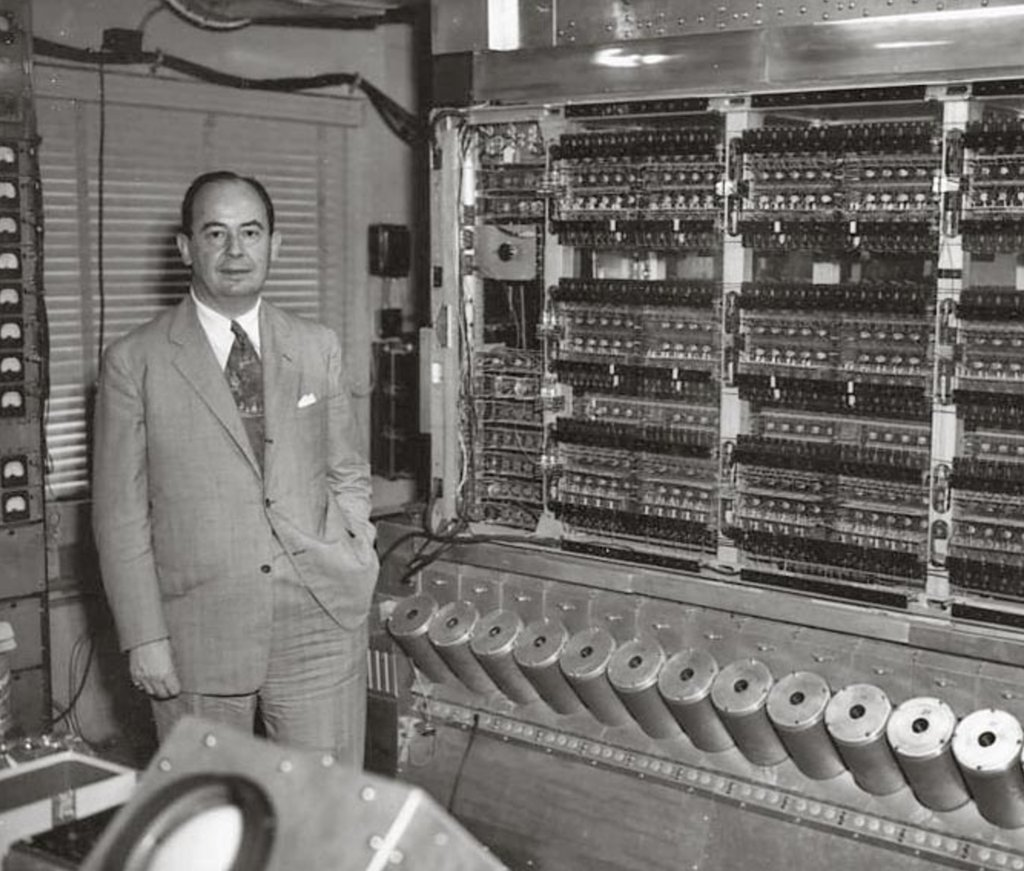
\includegraphics[width=11.5cm]{../resources/jpg/2.2.set.operations/neumann.jpg}
    \caption*{John Von Neumann in Turing's Cathedral.}
\end{figure}
\vspace{-1\baselineskip}
\subsection[Gamma is pi.]
    {
        \color{section}Theorem 61 \color{black} : gamma is pi.
    }
\documentclass[preview]{standalone}
\usepackage{amssymb, amsthm}
\usepackage{mathtools}
\usepackage{bm}


\newtheorem{theorem}{Theorem}
\renewcommand\qedsymbol{$\blacksquare$}


\begin{document}


\begin{theorem}[\textbf{2241}]
    Let \bm{$\Gamma$}, \bm{$\Pi$}, and \bm{$\Xi$} be sets.
    \begin{equation*}
        \bm{ \text{If }
            \Gamma \oplus \Xi 
                = 
            \Pi \oplus \Xi
                \text{, then } 
            \Gamma = \Pi
        }    
    \end{equation*}
\end{theorem}
\begin{proof} 
By contraposition. Note that the statement 
\bm{$
    \Gamma \oplus \Xi 
        = 
    \Pi \oplus \Xi
$}
is by definition 
\begin{equation*}
    \Big \langle \Gamma \cap \overline{\Xi} \Big \rangle 
        \cup 
    \Big \langle \overline{\Gamma} \cap \Xi \Big \rangle 
        \equiv
    \Big \langle \Pi \cap \overline{\Xi} \Big \rangle 
        \cup 
    \Big \langle \overline{\Pi} \cap \Xi \Big \rangle
\end{equation*}
Assume there exists an element \bm{$\zeta$} 
such that \bm{$\zeta \in \Gamma$} and \bm{$\zeta \notin \Pi$}. 
Thus, \bm{$\Gamma \nsubseteq \Pi$},
the negation of the consequent, by the definiton of subsets. 
By that hypothesis, 
\bm{$\zeta$} has to be in 
\bm{$\Gamma \cap \overline{\Xi}$} 
and cannot be in 
\bm{$\overline{\Gamma} \cap \Xi$}. 
This means that \bm{$\zeta$} is not in \bm{$\Xi$}. 
Neither can \bm{$\zeta$} be in 
\bm{$\Pi \cap \overline{\Xi}$}. 
And since \bm{$\zeta \notin \Xi$}, 
\bm{$\zeta$} cannot be in \bm{$\overline{\Pi} \cap \Xi$}. 
So \bm{$\zeta$} is in \bm{$\Gamma \oplus \Xi$} 
but not \bm{$\Pi \oplus \Xi$}. 
Therefore, 
\bm{$\Gamma \oplus \Xi \nsubseteq \Pi \oplus \Xi$},
by the definition of subsets.
The implication,
\begin{equation*}
    \Big \langle \Pi \not \subseteq \Gamma \Big \rangle
        \rightarrow
    \bigg[
        \Big \langle \Pi \oplus \Xi \Big \rangle
            \not \subseteq 
        \Big \langle \Gamma \oplus \Xi \Big \rangle
    \bigg]
\end{equation*} 
follows without loss of generality
$\therefore \text{\space} \bm{
    \Gamma \neq \Pi}$ 
implies 
\bm{$\Gamma \oplus \Xi \neq \Pi \oplus \Xi
}$.
\end{proof}


\end{document}
\pagebreak


\section{Lemmas}
\begin{figure}[!h]
    \centering
    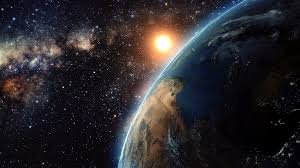
\includegraphics[width=14cm]{../resources/jpg/2.2.set.operations/sun.jpg}
\end{figure}


% =============================== 0001 Lemma 2201 =================================
\subsection{\color{section}Lemma 1}
\documentclass[preview]{standalone}
\usepackage{amssymb, amsthm}
\usepackage{mathtools}
\usepackage{bm}


\newtheorem{lemma}{Lemma}
\renewcommand\qedsymbol{$\blacksquare$}


\begin{document}


\begin{lemma}%[\textbf{2201}]
    Let \bm{$\mathrm{A}$}, and \bm{$\Lambda$} be sets.
    \begin{equation*}
        \bm{
            \mathrm{A} \oplus \Lambda
                =
            \Big \langle \mathrm{A} \cup \Lambda \Big \rangle
                \cap
            \Big \langle 
                \overline{\mathrm{A}} 
                    \cup 
                \overline{\Lambda} 
            \Big \rangle
        }
    \end{equation*}
\end{lemma}
\begin{proof}
    By Theorem 52,
    \bm{$
        \big \langle \mathrm{A} \oplus \Lambda \big \rangle
            \equiv
        \big \langle \mathrm{A} \cup \Lambda \big \rangle
            -
        \big \langle \mathrm{A} \cap \Lambda \big \rangle
    $}, 
    and by Theorem 45, that is
    \bm{$
        \big \langle \mathrm{A} \cup \Lambda \big \rangle
            \cap
        \big \langle \overline{\mathrm{A} \cap \Lambda} \big \rangle
    $}.
    By Demorgans law for the complement of set intersection,
    \begin{equation*}
        \Big \langle \mathrm{A} \cup \Lambda \Big \rangle
            \cap
        \Big \langle \overline{\mathrm{A} \cap \Lambda} \Big \rangle
            \equiv
        \Big \langle \mathrm{A} \cup \Lambda \Big \rangle
            \cap
        \Big \langle \overline{\mathrm{A}} \cup \overline{\Lambda} \Big \rangle
    \end{equation*}
    $\therefore \text{\space} \bm{
    \mathrm{A} \oplus \Lambda
        =
    \big \langle \mathrm{A} \cup \Lambda \big \rangle
        \cap
    \big \langle 
        \overline{\mathrm{A}} 
            \cup 
        \overline{\Lambda} 
    \big \rangle}$
\end{proof}


\end{document}
\vspace{2\baselineskip}
\sep
\pagebreak


% =============================== 0002 Lemma 2202 =================================
\subsection{\color{section}Lemma 2}
\documentclass[preview]{standalone}
\usepackage{amssymb, amsthm}
\usepackage{mathtools}
\usepackage{bm}


\newtheorem{lemma}{Lemma}
\renewcommand\qedsymbol{$\blacksquare$}


\begin{document}


\begin{lemma} %[\textbf{2202}]
    Let \bm{$\mathrm{A}$}, and \bm{$\Lambda$} be sets.
    \begin{equation*}
        \bm{
            \bigg[
                \Big \langle \mathrm{A} \cup \Lambda \Big \rangle
                    \cap
                \Big \langle 
                    \overline{\mathrm{A}} 
                        \cup 
                    \overline{\Lambda} 
                \Big \rangle
            \bigg]
                \cup
            \Lambda
                =
            \mathrm{A} \cup \Lambda
        }
    \end{equation*}
\end{lemma}
\begin{proof}
    Let \bm{$\Omega$} be the universe.
    By the law of distribution for set union over intersection,
    and by the associative law for set union,
    \begin{equation*}
        \bigg[
            \Big \langle \mathrm{A} \cup \Lambda \Big \rangle
                \cap
            \Big \langle 
                \overline{\mathrm{A}} 
                    \cup 
                \overline{\Lambda} 
            \Big \rangle
        \Big]
            \cup
        \Lambda
            \equiv
        \Big \langle \mathrm{A} \cup \Lambda \cup \Lambda \Big \rangle
            \cap
        \Big \langle 
            \overline{\mathrm{A}} 
                \cup 
            \overline{\Lambda} 
                \cup
            \Lambda
        \Big \rangle
    \end{equation*}
    By the idempotent law for set union, 
    and by the complement law for set union, that is
    \begin{equation*}
        \Big \langle \mathrm{A} \cup \Lambda \Big \rangle
            \cap
        \Big \langle 
            \overline{\mathrm{A}} 
                \cup 
            \Omega
        \Big \rangle
    \end{equation*}
    The right-hand side of this intersection is dominated by the universe,
    according to the domination law for set union. Thus, that is
    \bm{$\mathrm{A} \cup \Lambda$} intersect \bm{$\Omega$}.
    $\therefore \text{\space} \bm{
    \big[
        \big \langle \mathrm{A} \cup \Lambda \big \rangle
            \cap
        \big \langle 
            \overline{\mathrm{A}} 
                \cup 
            \overline{\Lambda} 
        \big \rangle
    \big]
        \cup
    \Lambda
        =
    \mathrm{A} \cup \Lambda
    }$, by the identity law for the intersection of sets.
\end{proof}


\end{document}
\begin{figure}[!h]
    \centering
    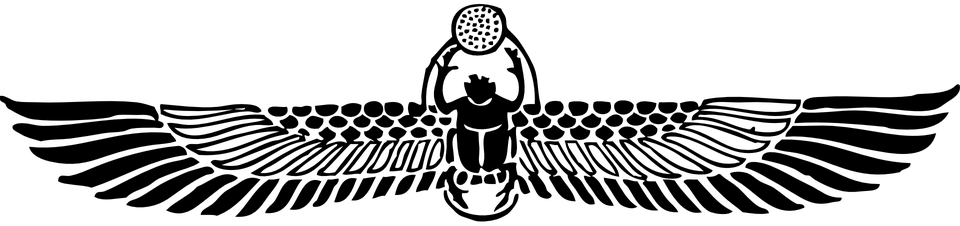
\includegraphics[width=8cm]{../resources/jpg/2.2.set.operations/scarab.png}
\end{figure}


% =============================== 0003 Lemma 2203 =================================
\subsection{\color{section}Lemma 3}
\documentclass[preview]{standalone}
\usepackage{amssymb, amsthm}
\usepackage{mathtools}
\usepackage{bm}


\newtheorem{lemma}{Lemma}
\renewcommand\qedsymbol{$\blacksquare$}


\begin{document}


\begin{lemma} %[\textbf{2203}]
    Let \bm{$\mathrm{A}$}, and \bm{$\Lambda$} be sets.
    \begin{equation*}
        \bm{
            \Big \langle \mathrm{A} \cup \Lambda \Big \rangle
                \cap
            \Big \langle 
                \overline{\mathrm{A}} 
                    \cup 
                \overline{\Lambda} 
            \Big \rangle
                \cap
            \Lambda
                =
            \Lambda \cap \overline{\mathrm{A}}
        }
    \end{equation*}
\end{lemma}
\begin{proof}
    By the law of distribution for set intersection over set union,
    \begin{equation*}
        \Big \langle \mathrm{A} \cup \Lambda \Big \rangle
            \cap
        \Big \langle 
            \overline{\mathrm{A}} 
                \cup 
            \overline{\Lambda} 
        \Big \rangle
            \cap
        \Lambda
            =
        \Big \langle \mathrm{A} \cup \Lambda \Big \rangle
            \cap
        \bigg[
            \Big \langle \overline{\mathrm{A}} \cap \Lambda \Big \rangle
                \cup
            \Big \langle \overline{\Lambda} \cap \Lambda \Big \rangle
        \bigg]
    \end{equation*}
    \bm{$\overline{\Lambda} \cap \Lambda \equiv \varnothing$}, 
    by the complement law for set intersection. 
    Therefore, the term in the brackets is \bm{$\overline{\mathrm{A}} \cap \Lambda$},
    by the identity law for set union. By the associative law for set intersection, what we have left is
    \begin{equation*}
        \Big \langle \mathrm{A} \cup \Lambda \Big \rangle
            \cap
        \overline{\mathrm{A}}
            \cap
        \Lambda
    \end{equation*}
    \bm{$\mathrm{A} \cup \Lambda$} is absorbed by \bm{$\Lambda$}, 
    by the absorption laws for sets, 
    since sets are commutative over intersection, 
    by the commutative law for set intersection.
    $\therefore \text{} \bm{
        \big \langle \mathrm{A} \cup \Lambda \big \rangle
            \cap
        \big \langle 
            \overline{\mathrm{A}} 
                \cup 
            \overline{\Lambda} 
        \big \rangle
            \cap
        \Lambda
            =
        \Lambda \cap \overline{\mathrm{A}}
    }$. 
\end{proof}


\end{document}
\pagebreak


% =============================== 0004 Lemma 2204 =================================
\subsection{\color{section}Lemma 4}
\documentclass[preview]{standalone}
\usepackage{amssymb, amsthm}
\usepackage{mathtools}
\usepackage{bm}


\newtheorem{lemma}{Lemma}
\renewcommand\qedsymbol{$\blacksquare$}


\begin{document}


\begin{lemma} %[\textbf{2204}]
    Let \bm{$\Gamma$}, \bm{$\Pi$}, and \bm{$\Xi$} be sets.
    \begin{equation*}
    \bm{
        \Big \langle \Gamma \cup \Pi \Big \rangle
            \cap
        \Big \langle \overline{\Gamma} \cup \overline{\Pi} \Big \rangle
            \cap
        \overline{\Xi}
            =
        \Big \langle \Pi \cap \overline{\Gamma} \cap \overline{\Xi} \Big \rangle
            \cup
        \Big \langle \Gamma \cap \overline{\Pi} \cap \overline{\Xi} \Big \rangle
        }
    \end{equation*}
\end{lemma}
\begin{proof}
    Distributing the term \bm{$\Gamma \cup \Pi$} over the union of 
    \bm{$\overline{\Gamma}$} and \bm{$\overline{\Pi}$},
    by the law of distribution for the intersection of sets over union,
    in the left-hand side of the equation expressed by the lemma is
    \begin{equation*}
        \bigg[
            \Big \langle \Gamma \cup \Pi \Big \rangle
                \cap
            \overline{\Gamma}
        \bigg]
            \cup
        \bigg[
            \Big \langle \Gamma \cup \Pi \Big \rangle
                \cap
            \overline{\Pi}
        \bigg]
            \cap
        \overline{\Xi}
    \end{equation*}
    Again, by the law of distribution for intersection over set union,
    \begin{equation*}
        \equiv
        \bigg[
            \Big \langle \Gamma \cap \overline{\Gamma} \Big \rangle
                \cup
            \Big \langle \Pi \cap \overline{\Gamma} \Big \rangle
        \bigg]
            \cup
        \bigg[
            \Big \langle \Gamma \cap \overline{\Pi} \Big \rangle
                \cup
            \Big \langle \Pi \cap \overline{\Pi} \Big \rangle
        \bigg]
            \cap
        \overline{\Xi}
    \end{equation*}
    \bm{$\Gamma \cap \overline{\Gamma}$} and \bm{$\Pi \cap \overline{\Pi}$}
    are both empty, by the domination law for set intersection. And any set,
    union the empty set, is itself, by the identity law for set union. Thus,
    by association, what is left is
    \begin{equation*}       
        \bigg[
            \Big \langle \Pi \cap \overline{\Gamma} \Big \rangle
                \cup
            \Big \langle \Gamma \cap \overline{\Pi} \Big \rangle
        \bigg]
            \cap
        \overline{\Xi}
    \end{equation*}
    $\therefore \bm{
        \big \langle \Gamma \cup \Pi \big \rangle
            \cap
        \big \langle \overline{\Gamma} \cup \overline{\Pi} \big \rangle
            \cap
        \overline{\Xi}
            =
        \big \langle \Pi \cap \overline{\Gamma} \cap \overline{\Xi} \big \rangle
            \cup
        \big \langle \Gamma \cap \overline{\Pi} \cap \overline{\Xi} \big \rangle
    }$,
    by the law of distribution for set intersection over set union,
    and by association for the intersection of sets.
\end{proof}


\end{document}
\sep
\vspace{1.5\baselineskip}
\begin{figure}[!h]
    \centering
    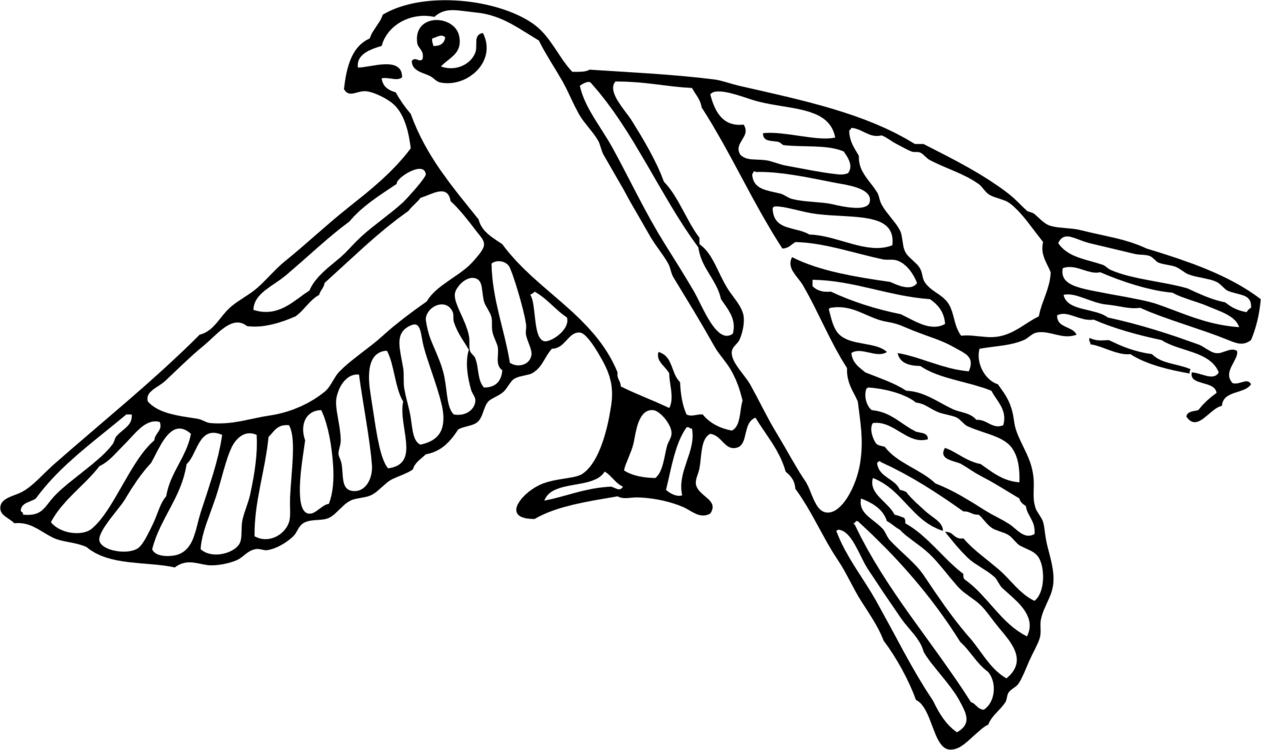
\includegraphics[width=8cm]{../resources/jpg/2.2.set.operations/bird.png}
\end{figure}
\pagebreak



% =============================== 0005 Lemma 2205 =================================
\subsection{\color{section}Lemma 5}
\documentclass[preview]{standalone}
\usepackage{amssymb, amsthm}
\usepackage{mathtools}
\usepackage{bm}


\newtheorem{lemma}{Lemma}
\renewcommand\qedsymbol{$\blacksquare$}


\begin{document}


\begin{lemma} %[\textbf{2205}]
    Let \bm{$\Gamma$}, \bm{$\Pi$}, and \bm{$\Xi$} be sets.
    \begin{equation*}
        \bm{
            \overline{
                \Big \langle \Gamma \cup \Pi \Big \rangle
                    \cap
                \Big \langle \overline{\Gamma} \cup \overline{\Pi} \Big \rangle
            }
                \cap
            \Xi
                    =
            \Big \langle \overline{\Gamma} \cap \overline{\Pi} \cap \Xi \Big \rangle
                \cup
            \Big \langle \Gamma \cap \Pi \cap \Xi \Big \rangle
        }
    \end{equation*}
\end{lemma}
\begin{proof}
    By DeMorgans Law for sets, 
    the expression occurring in the left-hand side of the equation in the lemma is
    \begin{equation*}
        \bigg[
            \Big \langle \overline{\Gamma \cup \Pi} \Big \rangle
                \cup
            \Big \langle \overline{\overline{\Gamma} \cup \overline{\Pi}} \Big \rangle
        \bigg]
            \cap
        \Xi
    \end{equation*}
    Which, again by DeMorgans law for sets, and by the complementation law for sets, is equivalent to
    \begin{equation*}
        \bigg[
            \Big \langle \overline{\Gamma} \cap \overline{\Pi} \Big \rangle
                \cup
            \Big \langle \Gamma \cap \Pi \Big \rangle
        \bigg]
            \cap
        \Xi
    \end{equation*}
    By the distributive law for set intersection over set union,
    and by associative law for the intersection of sets, that is
    \begin{equation*}
        \Big \langle \overline{\Gamma} \cap \overline{\Pi} \cap \Xi \Big \rangle
            \cup
        \Big \langle \Gamma \cap \Pi \cap \Xi \Big \rangle
    \end{equation*}
    $\therefore \bm{
        \overline{
            \big \langle \Gamma \cup \Pi \big \rangle
                \cap
            \big \langle \overline{\Gamma} \cup \overline{\Pi} \big \rangle
        }
            \cap
        \Xi
            =
        \big \langle \overline{\Gamma} \cap \overline{\Pi} \cap \Xi \big \rangle
            \cup
        \big \langle \Gamma \cap \Pi \cap \Xi \big \rangle
    }$.
\end{proof}


\end{document}
\sep
\pagebreak


\end{document}
\pagebreak


% ================================= Chapter 3 =================================
\chapter{Functions}
\documentclass[preview]{standalone}
%\documentclass[a4paper, 12pt]{article}
\usepackage{amssymb, amsthm}
\usepackage{mathtools}
\usepackage{bm}
\usepackage{xcolor}
\usepackage{standalone}


\newtheorem*{theorem*}{Theorem}
\newtheorem*{lemma*}{Lemma}

\renewcommand\qedsymbol{$\blacksquare$}


%\setcounter{page}{35}

\begin{document}


%\section*{2.3 Functions}
%\begin{center} \color{gray}
%    \rule{5.4in}{1pt}
%\end{center}


% ============================== Theorem 2320 ================================
\documentclass[preview]{standalone}
\usepackage{amssymb, amsthm}
\usepackage{mathtools}
\usepackage{bm}
\usepackage{xcolor}


\newtheorem*{theorem*}{Theorem}
\renewcommand\qedsymbol{$\blacksquare$}


\begin{document}


\begin{theorem*}[\textbf{2320}]
    Let \bm{$\gamma$} be the function \bm{$\gamma : \mathbb{R} \rightarrow \mathbb{R}$},
    such that
    \begin{equation*}
        \forall \alpha
            \Big \langle \gamma [ \alpha ] > 0 \Big \rangle
    \end{equation*}
    Let \bm{$\delta$} be the function \bm{$\delta: \mathbb{R} \rightarrow \mathbb{R}$} 
    defined by 
    \bm{$\delta [ \alpha ] = \frac{1}{\gamma[\alpha]}$}. 
    \bm{$\gamma[\alpha]$} is strictly increasing 
    if and only if 
    \bm{$\delta[\alpha]$} is strictly decreasing.
\end{theorem*}

\begin{proof}
    Suppose there exist real numbers \bm{$\alpha$} and \bm{$\beta$} such that 
    \bm{$\alpha < \beta$}, 
    and suppose that \bm{$\gamma[\alpha] < \gamma[\beta]$}. 
    \bm{$\gamma$} is a strictly increasing real-valued function by definition.
    By the multiplicative compatibility law from the order axioms, 
    multiplying both sides of the latter inequality by 
    \bm{$\frac{1}{\gamma[\alpha]\cdot\gamma[\beta]}$}
    \begin{equation*}
        \Bigg\{
            \left(
                \frac{\gamma[\alpha]}{\gamma[\alpha] \cdot \gamma[\beta]} 
            \right)
                    < 
            \left(
                \frac{\gamma[\beta]}{\gamma[\alpha] \cdot \gamma[\beta]}
            \right)
        \Bigg\}
            \equiv
        \Bigg\{
            \left(
                \frac{1}{\gamma[\beta]}
            \right)
                <
            \left(
                \frac{1}{\gamma[\alpha]}
            \right)
        \Bigg\}
            \equiv
    \end{equation*}
    \begin{equation*}
        \Bigg\{
            \bigg( \delta[\beta] \bigg)
                < 
            \bigg( \delta[\alpha] \bigg)
        \Bigg\}
    \end{equation*}
    Thus, \bm{$\delta$} is a strictly decreasing real-valued function,
    by definition. The converse can be proven by multiplying that inequality
    \bm{$\delta[\alpha] > \delta[\beta]$} by \bm{$\gamma[\alpha]\gamma[\beta]$},
    by the multiplicative compatibility law from the order axioms,
    \begin{equation*}
        \Bigg\{
            \left(
                \frac{1 \cdot \gamma[\alpha] \cdot \gamma[\beta]}{\gamma[\alpha]}
            \right)
                >
            \left(
                \frac{1 \cdot \gamma[\alpha] \cdot \gamma[\beta]}{\gamma[\beta]}
            \right)
        \Bigg\}
            \equiv
        \Bigg\{
            \bigg( \gamma[\beta] \bigg) 
                > 
            \bigg( \gamma[\alpha] \bigg)
        \Bigg\}
    \end{equation*}
    Thus, \bm{$\gamma$} is a strictly increasing real-valued function, by definition
    \bm{$\therefore \text{\space} \gamma[\alpha]$} is strictly increasing 
    if and only if 
    \bm{$\delta[\alpha]$} is strictly decreasing.
\color{lightgray} \end{proof}

\end{document}
%\documentclass[preview]{standalone}
\usepackage{amssymb, amsthm}
\usepackage{mathtools}
\usepackage{bm}
\usepackage{xcolor}


\newtheorem*{theorem*}{Theorem}
\renewcommand\qedsymbol{$\blacksquare$}


\begin{document}


\begin{theorem*}[\textbf{2320}]
    Let \bm{$\gamma$} be the function \bm{$\gamma : \mathbb{R} \rightarrow \mathbb{R}$},
    such that
    \begin{equation*}
        \forall \alpha
            \Big \langle \gamma [ \alpha ] > 0 \Big \rangle
    \end{equation*}
    Let \bm{$\delta$} be the function \bm{$\delta: \mathbb{R} \rightarrow \mathbb{R}$} 
    defined by 
    \bm{$\delta [ \alpha ] = \frac{1}{\gamma[\alpha]}$}. 
    \bm{$\gamma[\alpha]$} is strictly increasing 
    if and only if 
    \bm{$\delta[\alpha]$} is strictly decreasing.
\end{theorem*}

\begin{proof}
    Suppose there exist real numbers \bm{$\alpha$} and \bm{$\beta$} such that 
    \bm{$\alpha < \beta$}, 
    and suppose that \bm{$\gamma[\alpha] < \gamma[\beta]$}. 
    \bm{$\gamma$} is a strictly increasing real-valued function by definition.
    By the multiplicative compatibility law from the order axioms, 
    multiplying both sides of the latter inequality by 
    \bm{$\frac{1}{\gamma[\alpha]\cdot\gamma[\beta]}$}
    \begin{equation*}
        \Bigg\{
            \left(
                \frac{\gamma[\alpha]}{\gamma[\alpha] \cdot \gamma[\beta]} 
            \right)
                    < 
            \left(
                \frac{\gamma[\beta]}{\gamma[\alpha] \cdot \gamma[\beta]}
            \right)
        \Bigg\}
            \equiv
        \Bigg\{
            \left(
                \frac{1}{\gamma[\beta]}
            \right)
                <
            \left(
                \frac{1}{\gamma[\alpha]}
            \right)
        \Bigg\}
            \equiv
    \end{equation*}
    \begin{equation*}
        \Bigg\{
            \bigg( \delta[\beta] \bigg)
                < 
            \bigg( \delta[\alpha] \bigg)
        \Bigg\}
    \end{equation*}
    Thus, \bm{$\delta$} is a strictly decreasing real-valued function,
    by definition. The converse can be proven by multiplying that inequality
    \bm{$\delta[\alpha] > \delta[\beta]$} by \bm{$\gamma[\alpha]\gamma[\beta]$},
    by the multiplicative compatibility law from the order axioms,
    \begin{equation*}
        \Bigg\{
            \left(
                \frac{1 \cdot \gamma[\alpha] \cdot \gamma[\beta]}{\gamma[\alpha]}
            \right)
                >
            \left(
                \frac{1 \cdot \gamma[\alpha] \cdot \gamma[\beta]}{\gamma[\beta]}
            \right)
        \Bigg\}
            \equiv
        \Bigg\{
            \bigg( \gamma[\beta] \bigg) 
                > 
            \bigg( \gamma[\alpha] \bigg)
        \Bigg\}
    \end{equation*}
    Thus, \bm{$\gamma$} is a strictly increasing real-valued function, by definition
    \bm{$\therefore \text{\space} \gamma[\alpha]$} is strictly increasing 
    if and only if 
    \bm{$\delta[\alpha]$} is strictly decreasing.
\color{lightgray} \end{proof}

\end{document}
\pagebreak


% ============================== Theorem 2321 ================================
\documentclass[preview]{standalone}
\usepackage{amssymb, amsthm}
\usepackage{mathtools}
\usepackage{bm}
\usepackage{xcolor}


\newtheorem*{theorem*}{Theorem}
\renewcommand\qedsymbol{$\blacksquare$}


\begin{document}


\begin{theorem*}[\textbf{2321}]
    Let \bm{$\gamma$} be the function \bm{$\gamma : \mathbb{R} \rightarrow \mathbb{R}$}, such that 
    \begin{equation*}
        \forall \alpha \Big \langle
            \gamma[ \alpha ] > 0 \Big \rangle    
    \end{equation*} 
    Let \bm{$\delta$} be the function \bm{$\delta : \mathbb{R} \rightarrow \mathbb{R}$} 
    defined by \bm{$\delta[\alpha] = \frac{1}{\gamma[\alpha]}$}. 
    \bm{$\gamma[\alpha]$} is strictly decreasing 
    if and only if 
    \bm{$\delta[\alpha]$} is strictly increasing.
\end{theorem*}

\begin{proof}
    Suppose there exist real numbers \bm{$\alpha$} and \bm{$\beta$} such that 
    \bm{$\alpha < \beta$}, and suppose that 
    \bm{$\gamma[ \alpha ] > \gamma[ \beta ]$}. \bm{$\gamma$} is a strictly decreasing real-valued function by definition. 
    By the multiplicative compatibility law from the order axioms, 
    Multiplying both sides of the latter inequality by \bm{$\frac{1}{\gamma[\alpha] \cdot \gamma[\beta]}$}
    \begin{equation*}
        \Bigg\{
            \left(
                \frac{\gamma[\alpha]}{\gamma[\alpha] \cdot \gamma[\beta]}
            \right)
                >
            \left(
                \frac{\gamma[\beta]}{\gamma[\alpha] \cdot \gamma[\beta]}
            \right)  
        \Bigg\}
            \equiv
        \Bigg\{
            \left(
                \frac{1}{\gamma[\beta]}
            \right)
                >
            \left(
                \frac{1}{\gamma[\alpha]}
            \right)
        \Bigg\}
            \equiv
    \end{equation*}
    \begin{equation*}
        \Bigg\{
            \bigg(
                \delta[\beta]
            \bigg)
                >
            \bigg(
                \delta[\alpha]
            \bigg)
        \Bigg\}
    \end{equation*}
    Thus, \bm{$\delta$} is a strictly increasing real-valued function,
    by defintion.
    The converse can be proven by multiplying that inequality
    \bm{$\delta[\alpha] < \delta[\beta]$} by \bm{$\gamma[\alpha]\gamma[\beta]$},
    by the multiplicative compatibility law from the order axioms,
    \begin{equation*}
        \Bigg\{
            \bigg(
                \frac{1 \cdot \gamma[\alpha] \cdot \gamma[\beta]}{\gamma[\alpha]}
                    <
                \frac{1 \cdot \gamma[\alpha] \cdot \gamma[\beta]}{\gamma[\beta]}
            \bigg)
        \Bigg\}
            \equiv
        \Bigg\{
            \bigg(
                \gamma[\beta]
            \bigg)
                <
            \bigg(
                \gamma[\alpha]
            \bigg)
        \Bigg\} 
    \end{equation*}
    Thus, \bm{$\gamma$} is a strictly decreasing real-valued function, by defintion
    \bm{$\therefore \text{\space} \gamma[\alpha]$} is strictly decreasing
    if and only if
    \bm{$\delta[\alpha]$} is strictly increasing.
\color{lightgray} \end{proof}

\end{document}
%\documentclass[preview]{standalone}
\usepackage{amssymb, amsthm}
\usepackage{mathtools}
\usepackage{bm}
\usepackage{xcolor}


\newtheorem*{theorem*}{Theorem}
\renewcommand\qedsymbol{$\blacksquare$}


\begin{document}


\begin{theorem*}[\textbf{2321}]
    Let \bm{$\gamma$} be the function \bm{$\gamma : \mathbb{R} \rightarrow \mathbb{R}$}, such that 
    \begin{equation*}
        \forall \alpha \Big \langle
            \gamma[ \alpha ] > 0 \Big \rangle    
    \end{equation*} 
    Let \bm{$\delta$} be the function \bm{$\delta : \mathbb{R} \rightarrow \mathbb{R}$} 
    defined by \bm{$\delta[\alpha] = \frac{1}{\gamma[\alpha]}$}. 
    \bm{$\gamma[\alpha]$} is strictly decreasing 
    if and only if 
    \bm{$\delta[\alpha]$} is strictly increasing.
\end{theorem*}

\begin{proof}
    Suppose there exist real numbers \bm{$\alpha$} and \bm{$\beta$} such that 
    \bm{$\alpha < \beta$}, and suppose that 
    \bm{$\gamma[ \alpha ] > \gamma[ \beta ]$}. \bm{$\gamma$} is a strictly decreasing real-valued function by definition. 
    By the multiplicative compatibility law from the order axioms, 
    Multiplying both sides of the latter inequality by \bm{$\frac{1}{\gamma[\alpha] \cdot \gamma[\beta]}$}
    \begin{equation*}
        \Bigg\{
            \left(
                \frac{\gamma[\alpha]}{\gamma[\alpha] \cdot \gamma[\beta]}
            \right)
                >
            \left(
                \frac{\gamma[\beta]}{\gamma[\alpha] \cdot \gamma[\beta]}
            \right)  
        \Bigg\}
            \equiv
        \Bigg\{
            \left(
                \frac{1}{\gamma[\beta]}
            \right)
                >
            \left(
                \frac{1}{\gamma[\alpha]}
            \right)
        \Bigg\}
            \equiv
    \end{equation*}
    \begin{equation*}
        \Bigg\{
            \bigg(
                \delta[\beta]
            \bigg)
                >
            \bigg(
                \delta[\alpha]
            \bigg)
        \Bigg\}
    \end{equation*}
    Thus, \bm{$\delta$} is a strictly increasing real-valued function,
    by defintion.
    The converse can be proven by multiplying that inequality
    \bm{$\delta[\alpha] < \delta[\beta]$} by \bm{$\gamma[\alpha]\gamma[\beta]$},
    by the multiplicative compatibility law from the order axioms,
    \begin{equation*}
        \Bigg\{
            \bigg(
                \frac{1 \cdot \gamma[\alpha] \cdot \gamma[\beta]}{\gamma[\alpha]}
                    <
                \frac{1 \cdot \gamma[\alpha] \cdot \gamma[\beta]}{\gamma[\beta]}
            \bigg)
        \Bigg\}
            \equiv
        \Bigg\{
            \bigg(
                \gamma[\beta]
            \bigg)
                <
            \bigg(
                \gamma[\alpha]
            \bigg)
        \Bigg\} 
    \end{equation*}
    Thus, \bm{$\gamma$} is a strictly decreasing real-valued function, by defintion
    \bm{$\therefore \text{\space} \gamma[\alpha]$} is strictly decreasing
    if and only if
    \bm{$\delta[\alpha]$} is strictly increasing.
\color{lightgray} \end{proof}

\end{document}
\begin{center} \color{lightgray}
    \rule{5.4in}{0.1pt}
\end{center}


% ============================== Theorem 2324 ================================
\documentclass[preview]{standalone}
\usepackage{amssymb, amsthm}
\usepackage{mathtools}
\usepackage{bm}
\usepackage{xcolor}


\newtheorem*{theorem*}{Theorem}
\renewcommand\qedsymbol{$\blacksquare$}


\begin{document}


\begin{theorem*}[\textbf{2324}]
    Let \bm{$\alpha$} be the function 
    \bm{$\alpha: \mathbb{R} \rightarrow \mathbb{R}$}
    defined by \bm{$\alpha[\lambda] = \epsilon ^\lambda$}. 
    \bm{$\alpha[\lambda]$} is not invertible.
\end{theorem*}

\begin{proof}
    \begin{equation*}
        \Big \langle \alpha[\lambda] = \epsilon ^\lambda \Big \rangle
            \rightarrow
        \bigg[
            \Big \langle \alpha ^{-1}[\lambda] \Big \rangle 
                =
            \Big \langle \log_{\epsilon} \lambda \Big \rangle
        \bigg]
    \end{equation*}
    The domain for \bm{$\alpha ^{-1}[\lambda]$} is \bm{$\mathbb{R}$}, by definition. 
    But logarithmic functions are undefined for negative-valued domains.
    Thus, \bm{$\alpha[\lambda]$} cannot be bijective, 
    so \bm{$\alpha[\lambda]$} is not invertible.
\color{lightgray} \end{proof}

\end{document}
%\documentclass[preview]{standalone}
\usepackage{amssymb, amsthm}
\usepackage{mathtools}
\usepackage{bm}
\usepackage{xcolor}


\newtheorem*{theorem*}{Theorem}
\renewcommand\qedsymbol{$\blacksquare$}


\begin{document}


\begin{theorem*}[\textbf{2324}]
    Let \bm{$\alpha$} be the function 
    \bm{$\alpha: \mathbb{R} \rightarrow \mathbb{R}$}
    defined by \bm{$\alpha[\lambda] = \epsilon ^\lambda$}. 
    \bm{$\alpha[\lambda]$} is not invertible.
\end{theorem*}

\begin{proof}
    \begin{equation*}
        \Big \langle \alpha[\lambda] = \epsilon ^\lambda \Big \rangle
            \rightarrow
        \bigg[
            \Big \langle \alpha ^{-1}[\lambda] \Big \rangle 
                =
            \Big \langle \log_{\epsilon} \lambda \Big \rangle
        \bigg]
    \end{equation*}
    The domain for \bm{$\alpha ^{-1}[\lambda]$} is \bm{$\mathbb{R}$}, by definition. 
    But logarithmic functions are undefined for negative-valued domains.
    Thus, \bm{$\alpha[\lambda]$} cannot be bijective, 
    so \bm{$\alpha[\lambda]$} is not invertible.
\color{lightgray} \end{proof}

\end{document}
\begin{center} \color{lightgray}
    \rule{5.4in}{0.1pt}
\end{center}


% ============================== Theorem 2325 ================================
\documentclass[preview]{standalone}
\usepackage{amssymb, amsthm}
\usepackage{mathtools}
\usepackage{bm}
\usepackage{xcolor}


\newtheorem*{theorem*}{Theorem}
\renewcommand\qedsymbol{$\blacksquare$}


\begin{document}


\begin{theorem*}[\textbf{2325}]
    Let \bm{$\alpha$} be a function 
    \bm{$\alpha : \mathbb{R} \rightarrow \mathbb{R}$}
    defined by \bm{$\alpha[\lambda] = |\lambda|$}. 
    \bm{$\alpha[\lambda]$} is not invertible.
\end{theorem*}

\begin{proof}
    Let \bm{$\lambda$} be a postive real number. 
    By the definition for \bm{$\alpha$}, 
    \begin{equation*}
        \Big \langle \alpha[\lambda] = \lambda \Big \rangle
            \land
        \Big \langle \alpha[-1 \cdot \lambda] = \lambda \Big \rangle
    \end{equation*}
    So if \bm{$\alpha$} had an inverse, then
    \begin{equation*}
        \Big \langle \alpha ^{-1}[\lambda] = \lambda \Big \rangle
            \lor 
        \Big \langle \alpha ^{-1}[\lambda] = -1 \cdot \lambda \Big \rangle
    \end{equation*}
    Thus, \bm{$\alpha ^{-1}$} is not a function by definition.
\color{lightgray} \end{proof}

\end{document}
%\documentclass[preview]{standalone}
\usepackage{amssymb, amsthm}
\usepackage{mathtools}
\usepackage{bm}
\usepackage{xcolor}


\newtheorem*{theorem*}{Theorem}
\renewcommand\qedsymbol{$\blacksquare$}


\begin{document}


\begin{theorem*}[\textbf{2325}]
    Let \bm{$\alpha$} be a function 
    \bm{$\alpha : \mathbb{R} \rightarrow \mathbb{R}$}
    defined by \bm{$\alpha[\lambda] = |\lambda|$}. 
    \bm{$\alpha[\lambda]$} is not invertible.
\end{theorem*}

\begin{proof}
    Let \bm{$\lambda$} be a postive real number. 
    By the definition for \bm{$\alpha$}, 
    \begin{equation*}
        \Big \langle \alpha[\lambda] = \lambda \Big \rangle
            \land
        \Big \langle \alpha[-1 \cdot \lambda] = \lambda \Big \rangle
    \end{equation*}
    So if \bm{$\alpha$} had an inverse, then
    \begin{equation*}
        \Big \langle \alpha ^{-1}[\lambda] = \lambda \Big \rangle
            \lor 
        \Big \langle \alpha ^{-1}[\lambda] = -1 \cdot \lambda \Big \rangle
    \end{equation*}
    Thus, \bm{$\alpha ^{-1}$} is not a function by definition.
\color{lightgray} \end{proof}

\end{document}
\pagebreak


% ============================== Theorem 2329a ================================
\documentclass[preview]{standalone}
\usepackage{amssymb, amsthm}
\usepackage{mathtools}
\usepackage{bm}
\usepackage{xcolor}


\newtheorem*{theorem*}{Theorem}
\renewcommand\qedsymbol{$\blacksquare$}


\begin{document}


\begin{theorem*}[\textbf{2329a}]
    Let \bm{$\lambda$} be a function 
    \bm{$\lambda: \Delta \rightarrow \mathrm{A}$}, 
    and let \bm{$\epsilon$} be a function 
    \bm{$\epsilon: \Lambda \rightarrow \Delta$}. 
    If both \bm{$\lambda$} and \bm{$\epsilon$} are injective, 
    then \bm{$\big \langle \lambda \circ \epsilon \big \rangle$} is injective.
\end{theorem*}

\begin{proof}
    By the contrapositive.
    Suppose it were not the case that 
    \bm{$\big \langle \lambda \circ \epsilon \big \rangle$}
    were injective. 
    By the definition for injective functions, 
    with domain of discourse 
    \bm{$\big \langle \iota, \zeta \in \Lambda \big \rangle$}, that is
    \begin{equation*}
        \lnot \forall \iota \forall \zeta \bigg \langle 
            \Big[
                \big \langle \lambda \circ \epsilon \big \rangle [\iota] 
                    = 
                \big \langle \lambda \circ \epsilon \big \rangle [\zeta] 
            \Big]
                \rightarrow 
            \big \langle \iota = \zeta \big \rangle 
        \bigg \rangle
    \end{equation*}
    The composition of functions 
    \bm{$\big \langle \lambda \circ \epsilon \big \rangle [\iota]$} 
    is defined as \bm{$\lambda \big[ \epsilon (\iota) \big]$}. 
    Thus, we have the equivalent universal quantification
    \begin{equation*}
        \lnot \forall \iota \forall \zeta \bigg \langle 
            \Big[
                \lambda \big[ \epsilon (\iota) \big] 
                    = 
                \lambda \big[ \epsilon (\zeta) \big] 
            \Big]
                \rightarrow
            \big \langle \iota = \zeta \big \rangle
        \bigg \rangle
    \end{equation*}
    In other words, it follows from the negation of the direct consequent that 
    it is not the case that \bm{$\lambda$} is injective, 
    by the definition for injective functions. 
    This is sufficient to prove the logical negation of the direct hypothesis. 
    Thus, if both \bm{$\lambda$} and \bm{$\epsilon$} are injective, 
    then 
    \bm{$\big \langle \lambda \circ \epsilon \big \rangle$} 
    is injective.
\color{lightgray} \end{proof}

\end{document}
%\documentclass[preview]{standalone}
\usepackage{amssymb, amsthm}
\usepackage{mathtools}
\usepackage{bm}
\usepackage{xcolor}


\newtheorem*{theorem*}{Theorem}
\renewcommand\qedsymbol{$\blacksquare$}


\begin{document}


\begin{theorem*}[\textbf{2329a}]
    Let \bm{$\lambda$} be a function 
    \bm{$\lambda: \Delta \rightarrow \mathrm{A}$}, 
    and let \bm{$\epsilon$} be a function 
    \bm{$\epsilon: \Lambda \rightarrow \Delta$}. 
    If both \bm{$\lambda$} and \bm{$\epsilon$} are injective, 
    then \bm{$\big \langle \lambda \circ \epsilon \big \rangle$} is injective.
\end{theorem*}

\begin{proof}
    By the contrapositive.
    Suppose it were not the case that 
    \bm{$\big \langle \lambda \circ \epsilon \big \rangle$}
    were injective. 
    By the definition for injective functions, 
    with domain of discourse 
    \bm{$\big \langle \iota, \zeta \in \Lambda \big \rangle$}, that is
    \begin{equation*}
        \lnot \forall \iota \forall \zeta \bigg \langle 
            \Big[
                \big \langle \lambda \circ \epsilon \big \rangle [\iota] 
                    = 
                \big \langle \lambda \circ \epsilon \big \rangle [\zeta] 
            \Big]
                \rightarrow 
            \big \langle \iota = \zeta \big \rangle 
        \bigg \rangle
    \end{equation*}
    The composition of functions 
    \bm{$\big \langle \lambda \circ \epsilon \big \rangle [\iota]$} 
    is defined as \bm{$\lambda \big[ \epsilon (\iota) \big]$}. 
    Thus, we have the equivalent universal quantification
    \begin{equation*}
        \lnot \forall \iota \forall \zeta \bigg \langle 
            \Big[
                \lambda \big[ \epsilon (\iota) \big] 
                    = 
                \lambda \big[ \epsilon (\zeta) \big] 
            \Big]
                \rightarrow
            \big \langle \iota = \zeta \big \rangle
        \bigg \rangle
    \end{equation*}
    In other words, it follows from the negation of the direct consequent that 
    it is not the case that \bm{$\lambda$} is injective, 
    by the definition for injective functions. 
    This is sufficient to prove the logical negation of the direct hypothesis. 
    Thus, if both \bm{$\lambda$} and \bm{$\epsilon$} are injective, 
    then 
    \bm{$\big \langle \lambda \circ \epsilon \big \rangle$} 
    is injective.
\color{lightgray} \end{proof}

\end{document}
\begin{center} \color{lightgray}
    \rule{5.4in}{0.1pt}
\end{center}


% ============================== Theorem 2329b ================================
\documentclass[preview]{standalone}
\usepackage{amssymb, amsthm}
\usepackage{mathtools}
\usepackage{bm}
\usepackage{xcolor}


\newtheorem*{theorem*}{Theorem}
\renewcommand\qedsymbol{$\blacksquare$}


\begin{document}


\begin{theorem*}[\textbf{2329b}]
    Let \bm{$\delta$} be a function 
    \bm{$\delta: \Delta \rightarrow \mathrm{A}$}, 
    and let \bm{$\gamma$} be a function 
    \bm{$\gamma : \Lambda \rightarrow \Delta$}. 
    If both \bm{$\delta$} and \bm{$\gamma$} are surjective, 
    then 
    \bm{$\big \langle \delta \circ \gamma \big \rangle$} 
    is surjective.
\end{theorem*}

\begin{proof}
    By the contrapositive. 
    Suppose it were not the case that
    \bm{$\big \langle \delta \circ \gamma \big \rangle$} 
    were surjective. 
    By the definition for surjective functions,
    with domain of discourse \bm{$\lambda \in \Lambda$} 
    and \bm{$\alpha \in \mathrm{A}$}, 
    that is
    \begin{equation*}
        \lnot \forall \alpha \exists \lambda \Big \langle
            \big \langle \delta \circ \gamma \big \rangle [\lambda] 
                = 
            \alpha
        \Big \rangle
    \end{equation*}
    The composition of functions 
    \bm{$\big \langle \delta \circ \gamma \big \rangle [\lambda]$} 
    is defined as \bm{$\delta \big[ \gamma(\lambda) \big]$}.
    Thus, we have the equivalent universal quantification
    \begin{equation*}
        \lnot \forall \alpha \exists \lambda \Big \langle
            \delta \big[ \gamma (\lambda) \big] = \alpha \Big \rangle
    \end{equation*}
    In other words, it follows from the negation of the direct consequent 
    that it is not the case that \bm{$\delta$} is surjective, 
    by the definition for surjective functions.
    This is sufficient to prove the logical negation of the direct hypothesis.
    Thus, if both \bm{$\delta$} and \bm{$\gamma$} are surjective, 
    then \bm{$\big \langle \delta \circ \gamma \big \rangle$} is surjective.
\color{lightgray} \end{proof}

\end{document}
%\documentclass[preview]{standalone}
\usepackage{amssymb, amsthm}
\usepackage{mathtools}
\usepackage{bm}
\usepackage{xcolor}


\newtheorem*{theorem*}{Theorem}
\renewcommand\qedsymbol{$\blacksquare$}


\begin{document}


\begin{theorem*}[\textbf{2329b}]
    Let \bm{$\delta$} be a function 
    \bm{$\delta: \Delta \rightarrow \mathrm{A}$}, 
    and let \bm{$\gamma$} be a function 
    \bm{$\gamma : \Lambda \rightarrow \Delta$}. 
    If both \bm{$\delta$} and \bm{$\gamma$} are surjective, 
    then 
    \bm{$\big \langle \delta \circ \gamma \big \rangle$} 
    is surjective.
\end{theorem*}

\begin{proof}
    By the contrapositive. 
    Suppose it were not the case that
    \bm{$\big \langle \delta \circ \gamma \big \rangle$} 
    were surjective. 
    By the definition for surjective functions,
    with domain of discourse \bm{$\lambda \in \Lambda$} 
    and \bm{$\alpha \in \mathrm{A}$}, 
    that is
    \begin{equation*}
        \lnot \forall \alpha \exists \lambda \Big \langle
            \big \langle \delta \circ \gamma \big \rangle [\lambda] 
                = 
            \alpha
        \Big \rangle
    \end{equation*}
    The composition of functions 
    \bm{$\big \langle \delta \circ \gamma \big \rangle [\lambda]$} 
    is defined as \bm{$\delta \big[ \gamma(\lambda) \big]$}.
    Thus, we have the equivalent universal quantification
    \begin{equation*}
        \lnot \forall \alpha \exists \lambda \Big \langle
            \delta \big[ \gamma (\lambda) \big] = \alpha \Big \rangle
    \end{equation*}
    In other words, it follows from the negation of the direct consequent 
    that it is not the case that \bm{$\delta$} is surjective, 
    by the definition for surjective functions.
    This is sufficient to prove the logical negation of the direct hypothesis.
    Thus, if both \bm{$\delta$} and \bm{$\gamma$} are surjective, 
    then \bm{$\big \langle \delta \circ \gamma \big \rangle$} is surjective.
\color{lightgray} \end{proof}

\end{document}
\pagebreak


% ============================== Theorem 2330 ================================
\documentclass[preview]{standalone}
\usepackage{amssymb, amsthm}
\usepackage{mathtools}
\usepackage{bm}
\usepackage{xcolor}


\newtheorem*{theorem*}{Theorem}
\renewcommand\qedsymbol{$\blacksquare$}


\begin{document}


\begin{theorem*}[\textbf{2330}]
    Let \bm{$\delta$} and 
    \bm{$\big \langle \delta \circ \gamma \big \rangle$} 
    be injective functions.
    \bm{$\gamma$} is injective.
\end{theorem*}

\begin{proof}
    By the contrapositive. Suppose that \bm{$\gamma$} were not injective. 
    Then by the definition for injective functions we have the following universally quantified statement, 
    with the domain of discourse being the domain of \bm{$\gamma$},
    \begin{equation*}
        \lnot \forall \mu \forall \nu \Big \langle
            \big \langle \gamma [\mu] = \gamma [\nu] \big \rangle
                \rightarrow 
            \big \langle \mu = \nu \big \rangle
        \Big \rangle
    \end{equation*}
    By the equality properties for equations, and by the defintion for the composition of functions,
    \begin{equation*}
        \Big \langle
            \gamma[\mu] = \gamma[\nu] 
        \Big \rangle
            \rightarrow 
        \bigg\{
            \Big \langle
                \delta \big[ \gamma(\mu) \big] 
                    = 
                \delta \big[ \gamma(\nu) \big] 
            \Big \rangle
                \equiv 
            \Big[
                \big \langle \delta \circ \gamma \big \rangle [\mu] 
                    = 
                \big \langle \delta \circ \gamma \big \rangle [\nu]
            \Big]
        \bigg\}
    \end{equation*}
    Thus, the universal quantification above implies
    \begin{equation*}
        \lnot \forall \mu \forall \nu \bigg \langle
            \Big\{
                \big \langle \delta \circ \gamma \big \rangle [\mu] 
                    = 
                \big \langle \delta \circ \gamma \big \rangle [\nu]
            \Big\}
                \rightarrow
            \big \langle \mu = \nu \big \rangle
        \bigg \rangle
    \end{equation*}
    That is, 
    it is not the case that 
    \bm{$\big \langle \delta \circ \gamma \big \rangle$} is injective, by the definition for injective functions. 
    Since it follows directly from the negation of the consequent that 
    \bm{$\big \langle \delta \circ \gamma \big \rangle$} is not injective:
    if \bm{$\delta$} and 
    \bm{$\big \langle \delta \circ \gamma \big \rangle$} 
    are injective functions, 
    then \bm{$\gamma$} is indeed injective.
\color{lightgray} \end{proof}

\end{document}
%\documentclass[preview]{standalone}
\usepackage{amssymb, amsthm}
\usepackage{mathtools}
\usepackage{bm}
\usepackage{xcolor}


\newtheorem*{theorem*}{Theorem}
\renewcommand\qedsymbol{$\blacksquare$}


\begin{document}


\begin{theorem*}[\textbf{2330}]
    Let \bm{$\delta$} and 
    \bm{$\big \langle \delta \circ \gamma \big \rangle$} 
    be injective functions.
    \bm{$\gamma$} is injective.
\end{theorem*}

\begin{proof}
    By the contrapositive. Suppose that \bm{$\gamma$} were not injective. 
    Then by the definition for injective functions we have the following universally quantified statement, 
    with the domain of discourse being the domain of \bm{$\gamma$},
    \begin{equation*}
        \lnot \forall \mu \forall \nu \Big \langle
            \big \langle \gamma [\mu] = \gamma [\nu] \big \rangle
                \rightarrow 
            \big \langle \mu = \nu \big \rangle
        \Big \rangle
    \end{equation*}
    By the equality properties for equations, and by the defintion for the composition of functions,
    \begin{equation*}
        \Big \langle
            \gamma[\mu] = \gamma[\nu] 
        \Big \rangle
            \rightarrow 
        \bigg\{
            \Big \langle
                \delta \big[ \gamma(\mu) \big] 
                    = 
                \delta \big[ \gamma(\nu) \big] 
            \Big \rangle
                \equiv 
            \Big[
                \big \langle \delta \circ \gamma \big \rangle [\mu] 
                    = 
                \big \langle \delta \circ \gamma \big \rangle [\nu]
            \Big]
        \bigg\}
    \end{equation*}
    Thus, the universal quantification above implies
    \begin{equation*}
        \lnot \forall \mu \forall \nu \bigg \langle
            \Big\{
                \big \langle \delta \circ \gamma \big \rangle [\mu] 
                    = 
                \big \langle \delta \circ \gamma \big \rangle [\nu]
            \Big\}
                \rightarrow
            \big \langle \mu = \nu \big \rangle
        \bigg \rangle
    \end{equation*}
    That is, 
    it is not the case that 
    \bm{$\big \langle \delta \circ \gamma \big \rangle$} is injective, by the definition for injective functions. 
    Since it follows directly from the negation of the consequent that 
    \bm{$\big \langle \delta \circ \gamma \big \rangle$} is not injective:
    if \bm{$\delta$} and 
    \bm{$\big \langle \delta \circ \gamma \big \rangle$} 
    are injective functions, 
    then \bm{$\gamma$} is indeed injective.
\color{lightgray} \end{proof}

\end{document}
\begin{center} \color{lightgray}
    \rule{5.4in}{0.1pt}
\end{center}


% ============================== Theorem 2336a ===============================
\documentclass[preview]{standalone}
\usepackage{amssymb, amsthm}
\usepackage{mathtools}
\usepackage{bm}
\usepackage{xcolor}


\newtheorem*{theorem*}{Theorem}
\renewcommand\qedsymbol{$\blacksquare$}


\begin{document}


\begin{theorem*}[\textbf{2336a}]
    Let \bm{$\lambda$} be the function 
    \bm{$\lambda: \Gamma \to \Phi$}. 
    Let \bm{$\mathrm{A}$}, and \bm{$\Lambda$} be subsets of \bm{$\Gamma$}. 
    \begin{equation*}
        \bm{
            \lambda \big[ \mathrm{A} \cup \Lambda \big] 
                = 
            \lambda \big[ \mathrm{A} \big] \cup \lambda \big[ \Lambda \big]
        }
    \end{equation*}
\end{theorem*}

\begin{proof}
    Suppose there exists an element \bm{$\phi$} such that
    \bm{$\phi \in \lambda \big[ \mathrm{A} \cup \Lambda \big]$}.
    By the definition for the image of a set under the function \bm{$\lambda$},
    \bm{$\phi = \lambda \big[ \iota \big]$} 
    where \bm{$\iota$} is an element in \bm{$\mathrm{A} \cup \Lambda$}. 
    That is, by the definition for the union of sets,
    \bm{$\iota \in \mathrm{A} \lor \iota \in \Lambda$}. 
    Thus, 
    \bm{$\phi \in \lambda \big[ \mathrm{A} \big] \lor \phi \in \lambda \big[ \Lambda \big]$}.
    And by the definition for set union, 
    \bm{$\phi \in \lambda \big[ \mathrm{A} \big] \cup \lambda \big[ \Lambda \big]$}.
    
    Suppose there exists an element \bm{$\phi$} such that 
    \bm{$\phi \in \lambda \big[ \mathrm{A} \big] \cup \lambda \big[ \Lambda \big]$}.
    By the defintion for set union, 
    \bm{$\phi \in \lambda \big[ \mathrm{A} \big] \lor \phi \in \lambda \big[ \Lambda \big]$}.
    By the definition for the image of a set under the function \bm{$\lambda$},
    there exists an element \bm{$\iota \in \mathrm{A} \lor \iota \in \Lambda$} such that 
    \bm{$\lambda \big[ \iota \big] = \phi$}.
    By the definition for set union, 
    \bm{$\iota \in \mathrm{A} \cup \Lambda$}.
    Hence,
    \bm{$\phi \in \lambda \big[ \mathrm{A} \cup \Lambda \big]$}
\color{lightgray} \end{proof}

\end{document}
%\documentclass[preview]{standalone}
\usepackage{amssymb, amsthm}
\usepackage{mathtools}
\usepackage{bm}
\usepackage{xcolor}


\newtheorem*{theorem*}{Theorem}
\renewcommand\qedsymbol{$\blacksquare$}


\begin{document}


\begin{theorem*}[\textbf{2336a}]
    Let \bm{$\lambda$} be the function 
    \bm{$\lambda: \Gamma \to \Phi$}. 
    Let \bm{$\mathrm{A}$}, and \bm{$\Lambda$} be subsets of \bm{$\Gamma$}. 
    \begin{equation*}
        \bm{
            \lambda \big[ \mathrm{A} \cup \Lambda \big] 
                = 
            \lambda \big[ \mathrm{A} \big] \cup \lambda \big[ \Lambda \big]
        }
    \end{equation*}
\end{theorem*}

\begin{proof}
    Suppose there exists an element \bm{$\phi$} such that
    \bm{$\phi \in \lambda \big[ \mathrm{A} \cup \Lambda \big]$}.
    By the definition for the image of a set under the function \bm{$\lambda$},
    \bm{$\phi = \lambda \big[ \iota \big]$} 
    where \bm{$\iota$} is an element in \bm{$\mathrm{A} \cup \Lambda$}. 
    That is, by the definition for the union of sets,
    \bm{$\iota \in \mathrm{A} \lor \iota \in \Lambda$}. 
    Thus, 
    \bm{$\phi \in \lambda \big[ \mathrm{A} \big] \lor \phi \in \lambda \big[ \Lambda \big]$}.
    And by the definition for set union, 
    \bm{$\phi \in \lambda \big[ \mathrm{A} \big] \cup \lambda \big[ \Lambda \big]$}.
    
    Suppose there exists an element \bm{$\phi$} such that 
    \bm{$\phi \in \lambda \big[ \mathrm{A} \big] \cup \lambda \big[ \Lambda \big]$}.
    By the defintion for set union, 
    \bm{$\phi \in \lambda \big[ \mathrm{A} \big] \lor \phi \in \lambda \big[ \Lambda \big]$}.
    By the definition for the image of a set under the function \bm{$\lambda$},
    there exists an element \bm{$\iota \in \mathrm{A} \lor \iota \in \Lambda$} such that 
    \bm{$\lambda \big[ \iota \big] = \phi$}.
    By the definition for set union, 
    \bm{$\iota \in \mathrm{A} \cup \Lambda$}.
    Hence,
    \bm{$\phi \in \lambda \big[ \mathrm{A} \cup \Lambda \big]$}
\color{lightgray} \end{proof}

\end{document}
\begin{center} \color{lightgray}
    \rule{5.4in}{0.1pt}
\end{center}


% ============================== Theorem 2368 ================================
\documentclass[preview]{standalone}
\usepackage{amssymb, amsthm}
\usepackage{mathtools}
\usepackage{bm}
\usepackage{xcolor}


\newtheorem*{theorem*}{Theorem}
\renewcommand\qedsymbol{$\blacksquare$}


\begin{document}


\begin{theorem*}[\textbf{2368}]
    Let \bm{$\lambda$} be a function 
    \bm{$\lambda : \mathrm{A} \rightarrow \Lambda$}, 
    where \bm{$\mathrm{A}$} and \bm{$\mathrm{\Lambda}$} are finite sets, 
    and \bm{$|\mathrm{A}| = |\Lambda|$}. 
    \bm{$\lambda$} is injective 
    if and only if 
    \bm{$\lambda$} is surjective.
\end{theorem*}

\begin{proof}
    Direct form by the contrapositive. 
    Suppose \bm{$\lambda$} is not surjective. 
    This can be true only if \bm{$|\mathrm{A}| < |\Lambda|$} (which is impossible,) 
    or when \bm{$\lambda$} is not injective.
    Thus, if \bm{$\lambda$} is injective, then \bm{$\lambda$} is surjective.
    \\ \\
    Converse form by the contrapositive. Suppose \bm{$\lambda$} is not injective.
    This can be true only if \bm{$|\mathrm{A}| > |\Lambda|$} (which is impossible,) 
    or when \bm{$\lambda$} is not surjective. 
    Thus, if \bm{$\lambda$} is surjective, then \bm{$\lambda$} is injective.
\color{lightgray} \end{proof}

\end{document}
%\documentclass[preview]{standalone}
\usepackage{amssymb, amsthm}
\usepackage{mathtools}
\usepackage{bm}
\usepackage{xcolor}


\newtheorem*{theorem*}{Theorem}
\renewcommand\qedsymbol{$\blacksquare$}


\begin{document}


\begin{theorem*}[\textbf{2368}]
    Let \bm{$\lambda$} be a function 
    \bm{$\lambda : \mathrm{A} \rightarrow \Lambda$}, 
    where \bm{$\mathrm{A}$} and \bm{$\mathrm{\Lambda}$} are finite sets, 
    and \bm{$|\mathrm{A}| = |\Lambda|$}. 
    \bm{$\lambda$} is injective 
    if and only if 
    \bm{$\lambda$} is surjective.
\end{theorem*}

\begin{proof}
    Direct form by the contrapositive. 
    Suppose \bm{$\lambda$} is not surjective. 
    This can be true only if \bm{$|\mathrm{A}| < |\Lambda|$} (which is impossible,) 
    or when \bm{$\lambda$} is not injective.
    Thus, if \bm{$\lambda$} is injective, then \bm{$\lambda$} is surjective.
    \\ \\
    Converse form by the contrapositive. Suppose \bm{$\lambda$} is not injective.
    This can be true only if \bm{$|\mathrm{A}| > |\Lambda|$} (which is impossible,) 
    or when \bm{$\lambda$} is not surjective. 
    Thus, if \bm{$\lambda$} is surjective, then \bm{$\lambda$} is injective.
\color{lightgray} \end{proof}

\end{document}
\pagebreak


% ============================== Theorem 2336b ===============================
\documentclass[preview]{standalone}
\usepackage{amssymb, amsthm}
\usepackage{mathtools}
\usepackage{bm}
\usepackage{xcolor}


\newtheorem*{theorem*}{Theorem}
\renewcommand\qedsymbol{$\blacksquare$}


\begin{document}


\begin{theorem*}[\textbf{2.2.36b}]
    Let \bm{$\lambda$} be the function 
    \bm{$\lambda : \Gamma \rightarrow \Delta$}. 
    Let \bm{$\mathrm{A}$}, 
    and \bm{$\Lambda$} be subsets of \bm{$\Gamma$}.
    \begin{equation*}
        \bm{
            \Big \langle \lambda \big[ \mathrm{A} \cap \Lambda \big] \Big \rangle
                \subseteq 
            \Big \langle \lambda \big[ \mathrm{A} \big] \cap \lambda \big[ \Lambda \big] \Big \rangle
        }
    \end{equation*}
\end{theorem*}

\begin{proof}
    Let \bm{$\iota$} be an element in \bm{$\Gamma$} such that 
    \bm{$\lambda \big[ \iota \big]$} is a member of 
    \bm{$\lambda \big[ \mathrm{A} \cap \Lambda \big]$}. 
    By the definition for the image of 
    \bm{$\big \langle \mathrm{A} \cap \Lambda \big \rangle$} 
    under the function \bm{$\lambda$}, 
    \bm{$\iota$} is an element in 
    \bm{$\big \langle \mathrm{A} \cap \Lambda \big \rangle$}. 
    By the definition for the
    intersection of sets 
    \begin{equation*}
        \Big \langle \iota \in \mathrm{A} \Big \rangle 
            \land 
        \Big \langle \iota \in \Lambda \Big \rangle
    \end{equation*}
    Thus,
    \begin{equation*}
        \Big \langle 
            \lambda \big[ \iota \big] 
                \in 
            \lambda \big[ \mathrm{A} \big]
        \Big \rangle 
            \land 
        \Big \langle
            \lambda \big[ \iota \big] 
                \in 
            \lambda \big[ \Lambda \big]
        \Big \rangle
    \end{equation*} 
    By the definition for set intersection,
    \bm{$\lambda \big[ \iota \big]$} is a member of
    \bm{$
        \big \langle 
            \lambda \big[ \mathrm{A} \big] 
                \cap 
            \lambda \big[ \Lambda \big]
        \big \rangle    
    $},
    $\therefore \text{\space} \bm{
        \lambda \big[ \mathrm{A} \cap \Lambda \big] 
            \subseteq 
        \lambda \big[ \mathrm{A} \big] \cap \lambda \big[ \Lambda \big]
    }$.
\color{lightgray} \end{proof}

\end{document}
%\documentclass[preview]{standalone}
\usepackage{amssymb, amsthm}
\usepackage{mathtools}
\usepackage{bm}
\usepackage{xcolor}


\newtheorem*{theorem*}{Theorem}
\renewcommand\qedsymbol{$\blacksquare$}


\begin{document}


\begin{theorem*}[\textbf{2.2.36b}]
    Let \bm{$\lambda$} be the function 
    \bm{$\lambda : \Gamma \rightarrow \Delta$}. 
    Let \bm{$\mathrm{A}$}, 
    and \bm{$\Lambda$} be subsets of \bm{$\Gamma$}.
    \begin{equation*}
        \bm{
            \Big \langle \lambda \big[ \mathrm{A} \cap \Lambda \big] \Big \rangle
                \subseteq 
            \Big \langle \lambda \big[ \mathrm{A} \big] \cap \lambda \big[ \Lambda \big] \Big \rangle
        }
    \end{equation*}
\end{theorem*}

\begin{proof}
    Let \bm{$\iota$} be an element in \bm{$\Gamma$} such that 
    \bm{$\lambda \big[ \iota \big]$} is a member of 
    \bm{$\lambda \big[ \mathrm{A} \cap \Lambda \big]$}. 
    By the definition for the image of 
    \bm{$\big \langle \mathrm{A} \cap \Lambda \big \rangle$} 
    under the function \bm{$\lambda$}, 
    \bm{$\iota$} is an element in 
    \bm{$\big \langle \mathrm{A} \cap \Lambda \big \rangle$}. 
    By the definition for the
    intersection of sets 
    \begin{equation*}
        \Big \langle \iota \in \mathrm{A} \Big \rangle 
            \land 
        \Big \langle \iota \in \Lambda \Big \rangle
    \end{equation*}
    Thus,
    \begin{equation*}
        \Big \langle 
            \lambda \big[ \iota \big] 
                \in 
            \lambda \big[ \mathrm{A} \big]
        \Big \rangle 
            \land 
        \Big \langle
            \lambda \big[ \iota \big] 
                \in 
            \lambda \big[ \Lambda \big]
        \Big \rangle
    \end{equation*} 
    By the definition for set intersection,
    \bm{$\lambda \big[ \iota \big]$} is a member of
    \bm{$
        \big \langle 
            \lambda \big[ \mathrm{A} \big] 
                \cap 
            \lambda \big[ \Lambda \big]
        \big \rangle    
    $},
    $\therefore \text{\space} \bm{
        \lambda \big[ \mathrm{A} \cap \Lambda \big] 
            \subseteq 
        \lambda \big[ \mathrm{A} \big] \cap \lambda \big[ \Lambda \big]
    }$.
\color{lightgray} \end{proof}

\end{document}
\begin{center} \color{lightgray}
    \rule{5.4in}{0.1pt}
\end{center}


% ============================== Theorem 2340a ===============================
\documentclass[preview]{standalone}
\usepackage{amssymb, amsthm}
\usepackage{mathtools}
\usepackage{bm}
\usepackage{xcolor}


\newtheorem*{theorem*}{Theorem}
\renewcommand\qedsymbol{$\blacksquare$}


\begin{document}


\begin{theorem*}[\textbf{2340a}]
    Let \bm{$\lambda$} be the function 
    \bm{$\lambda : \Gamma \rightarrow \mathrm{A}$}. 
    Let \bm{$\Lambda$}, and \bm{$\Delta$} 
    be subsets of \bm{$\mathrm{A}$}.
    \begin{equation*}
        \bm{
        \lambda ^{-1} \big[ \Lambda \cup \Delta \big] 
            = 
        \lambda ^{-1} 
            \big[ \Lambda \big] 
                \cup 
            \lambda^{-1} \big[ \Delta \big]
        }
    \end{equation*}
\end{theorem*}

\begin{proof}
    Let \bm{$\iota$} be an element in \bm{$\lambda ^{-1} \big[ \Lambda \cup \Delta \big]$}.
    By the inverse function for
    \bm{$\lambda ^{-1}$}, 
    and by the definition for the union of sets, that is 
    \begin{equation*}
        \bigg \langle \lambda 
            \big[ \iota \big] 
                \in 
            \lambda \Big[ 
                \lambda ^{-1} \big[ \Lambda \cup \Delta \big]
            \Big]
        \bigg \rangle
            \equiv
        \bigg[
            \Big \langle \lambda \big[ \iota \big] \in \Lambda \Big \rangle
                \lor 
            \Big \langle \lambda \big[ \iota \big] \in \Delta \Big \rangle
        \bigg]
    \end{equation*}
    By \bm{$\lambda$} inverse, and by the definition for set union, that is
    \begin{equation*}
        \bigg[
            \Big \langle
                \iota \in \lambda^{-1} \big[ \Lambda \big] 
            \Big \rangle
                \lor 
            \Big \langle
                \iota \in \lambda^{-1} \big[ \Delta \big]
            \Big \rangle
        \bigg]
            \equiv
        \bigg[ 
            \iota \in \Big \langle
                \lambda ^{-1} \big[ \Lambda \big] 
                    \cup 
                \lambda ^{-1} \big[ \Delta \big]
            \Big \rangle
        \bigg]
    \end{equation*}
    $\therefore \text{\space} \bm{
    \lambda ^{-1} \big[ \Lambda \cup \Delta \big] 
        = 
    \lambda ^{-1} 
        \big[ \Lambda \big] 
            \cup 
        \lambda^{-1} \big[ \Delta \big]
    }$.
\color{lightgray} \end{proof}

\end{document}
%\documentclass[preview]{standalone}
\usepackage{amssymb, amsthm}
\usepackage{mathtools}
\usepackage{bm}
\usepackage{xcolor}


\newtheorem*{theorem*}{Theorem}
\renewcommand\qedsymbol{$\blacksquare$}


\begin{document}


\begin{theorem*}[\textbf{2340a}]
    Let \bm{$\lambda$} be the function 
    \bm{$\lambda : \Gamma \rightarrow \mathrm{A}$}. 
    Let \bm{$\Lambda$}, and \bm{$\Delta$} 
    be subsets of \bm{$\mathrm{A}$}.
    \begin{equation*}
        \bm{
        \lambda ^{-1} \big[ \Lambda \cup \Delta \big] 
            = 
        \lambda ^{-1} 
            \big[ \Lambda \big] 
                \cup 
            \lambda^{-1} \big[ \Delta \big]
        }
    \end{equation*}
\end{theorem*}

\begin{proof}
    Let \bm{$\iota$} be an element in \bm{$\lambda ^{-1} \big[ \Lambda \cup \Delta \big]$}.
    By the inverse function for
    \bm{$\lambda ^{-1}$}, 
    and by the definition for the union of sets, that is 
    \begin{equation*}
        \bigg \langle \lambda 
            \big[ \iota \big] 
                \in 
            \lambda \Big[ 
                \lambda ^{-1} \big[ \Lambda \cup \Delta \big]
            \Big]
        \bigg \rangle
            \equiv
        \bigg[
            \Big \langle \lambda \big[ \iota \big] \in \Lambda \Big \rangle
                \lor 
            \Big \langle \lambda \big[ \iota \big] \in \Delta \Big \rangle
        \bigg]
    \end{equation*}
    By \bm{$\lambda$} inverse, and by the definition for set union, that is
    \begin{equation*}
        \bigg[
            \Big \langle
                \iota \in \lambda^{-1} \big[ \Lambda \big] 
            \Big \rangle
                \lor 
            \Big \langle
                \iota \in \lambda^{-1} \big[ \Delta \big]
            \Big \rangle
        \bigg]
            \equiv
        \bigg[ 
            \iota \in \Big \langle
                \lambda ^{-1} \big[ \Lambda \big] 
                    \cup 
                \lambda ^{-1} \big[ \Delta \big]
            \Big \rangle
        \bigg]
    \end{equation*}
    $\therefore \text{\space} \bm{
    \lambda ^{-1} \big[ \Lambda \cup \Delta \big] 
        = 
    \lambda ^{-1} 
        \big[ \Lambda \big] 
            \cup 
        \lambda^{-1} \big[ \Delta \big]
    }$.
\color{lightgray} \end{proof}

\end{document}
\begin{center} \color{lightgray}
    \rule{5.4in}{1pt}
\end{center}


% ============================== Theorem 2340b ===============================
\documentclass[preview]{standalone}
\usepackage{amssymb, amsthm}
\usepackage{mathtools}
\usepackage{bm}
\usepackage{xcolor}


\newtheorem*{theorem*}{Theorem}
\renewcommand\qedsymbol{$\blacksquare$}


\begin{document}


\begin{theorem*}[\textbf{2340b}]
    Let \bm{$\lambda$} be the function 
    \bm{$\lambda : \Gamma \rightarrow \mathrm{A}$}. 
    Let \bm{$\Lambda$}, and \bm{$\Delta$} 
    be subsets of \bm{$\mathrm{A}$}. 
    \begin{equation*}
        \bm{
        \lambda ^{-1} \big[ \Lambda \cap \Delta \big] 
            = 
        \lambda ^{-1} 
            \big[ \Lambda \big] 
                \cap 
            \lambda^{-1} \big[ \Delta \big]
        }
    \end{equation*}
\end{theorem*}

\begin{proof}
    Let \bm{$\iota$} be an element in \bm{$\lambda ^{-1} \big[ \Lambda \cap \Delta \big]$}.
    By the inverse function for
    \bm{$\lambda ^{-1}$}, 
    and by the definition for the intersection of sets, that is 
    \begin{equation*}
        \bigg \langle \lambda 
            \big[ \iota \big] 
                \in 
            \lambda \Big[ 
                \lambda ^{-1} \big[ \Lambda \cap \Delta \big]
            \Big]
        \bigg \rangle
            \equiv
        \bigg[
            \Big \langle \lambda \big[ \iota \big] \in \Lambda \Big \rangle
                \land 
            \Big \langle \lambda \big[ \iota \big] \in \Delta \Big \rangle
        \bigg]
    \end{equation*}
    By \bm{$\lambda$} inverse, and by the definition for set intersection, that is
    \begin{equation*}
        \bigg[
            \Big \langle
                \iota \in \lambda^{-1} \big[ \Lambda \big] 
            \Big \rangle
                \land 
            \Big \langle
                \iota \in \lambda^{-1} \big[ \Delta \big]
            \Big \rangle
        \bigg]
            \equiv
        \bigg[ 
            \iota \in \Big \langle
                \lambda ^{-1} \big[ \Lambda \big] 
                    \cap 
                \lambda ^{-1} \big[ \Delta \big]
            \Big \rangle
        \bigg]
    \end{equation*}
    $\therefore \text{\space} \bm{
    \lambda ^{-1} \big[ \Lambda \cap \Delta \big] 
        = 
    \lambda ^{-1} 
        \big[ \Lambda \big] 
            \cap 
        \lambda^{-1} \big[ \Delta \big]
    }$.
\color{lightgray} \end{proof}

\end{document}
%\documentclass[preview]{standalone}
\usepackage{amssymb, amsthm}
\usepackage{mathtools}
\usepackage{bm}
\usepackage{xcolor}


\newtheorem*{theorem*}{Theorem}
\renewcommand\qedsymbol{$\blacksquare$}


\begin{document}


\begin{theorem*}[\textbf{2340b}]
    Let \bm{$\lambda$} be the function 
    \bm{$\lambda : \Gamma \rightarrow \mathrm{A}$}. 
    Let \bm{$\Lambda$}, and \bm{$\Delta$} 
    be subsets of \bm{$\mathrm{A}$}. 
    \begin{equation*}
        \bm{
        \lambda ^{-1} \big[ \Lambda \cap \Delta \big] 
            = 
        \lambda ^{-1} 
            \big[ \Lambda \big] 
                \cap 
            \lambda^{-1} \big[ \Delta \big]
        }
    \end{equation*}
\end{theorem*}

\begin{proof}
    Let \bm{$\iota$} be an element in \bm{$\lambda ^{-1} \big[ \Lambda \cap \Delta \big]$}.
    By the inverse function for
    \bm{$\lambda ^{-1}$}, 
    and by the definition for the intersection of sets, that is 
    \begin{equation*}
        \bigg \langle \lambda 
            \big[ \iota \big] 
                \in 
            \lambda \Big[ 
                \lambda ^{-1} \big[ \Lambda \cap \Delta \big]
            \Big]
        \bigg \rangle
            \equiv
        \bigg[
            \Big \langle \lambda \big[ \iota \big] \in \Lambda \Big \rangle
                \land 
            \Big \langle \lambda \big[ \iota \big] \in \Delta \Big \rangle
        \bigg]
    \end{equation*}
    By \bm{$\lambda$} inverse, and by the definition for set intersection, that is
    \begin{equation*}
        \bigg[
            \Big \langle
                \iota \in \lambda^{-1} \big[ \Lambda \big] 
            \Big \rangle
                \land 
            \Big \langle
                \iota \in \lambda^{-1} \big[ \Delta \big]
            \Big \rangle
        \bigg]
            \equiv
        \bigg[ 
            \iota \in \Big \langle
                \lambda ^{-1} \big[ \Lambda \big] 
                    \cap 
                \lambda ^{-1} \big[ \Delta \big]
            \Big \rangle
        \bigg]
    \end{equation*}
    $\therefore \text{\space} \bm{
    \lambda ^{-1} \big[ \Lambda \cap \Delta \big] 
        = 
    \lambda ^{-1} 
        \big[ \Lambda \big] 
            \cap 
        \lambda^{-1} \big[ \Delta \big]
    }$.
\color{lightgray} \end{proof}

\end{document}
\pagebreak


% ============================== Theorem 2341 ================================
\documentclass[preview]{standalone}
\usepackage{amssymb, amsthm}
\usepackage{mathtools}
\usepackage{bm}
\usepackage{xcolor}


\newtheorem*{theorem*}{Theorem}
\renewcommand\qedsymbol{$\blacksquare$}


\begin{document}


\begin{theorem*}[\textbf{2341}]
    Let \bm{$\lambda$} be the function 
    \bm{$\lambda : \Delta \rightarrow \mathrm{A}$}. 
    Let \bm{$\Lambda$} be a subset of \bm{$\mathrm{A}$}. 
    \begin{equation*}
        \bm{
        \lambda ^{-1} \big[ \overline{\Lambda} \big] 
            = 
        \overline{ \lambda ^{-1} \big[ \Lambda \big]}
        }
    \end{equation*}
\end{theorem*}

\begin{proof}
    Let \bm{$\alpha$} be an element in 
    \bm{$\lambda ^{-1} \big[ \overline{\Lambda} \big]$}.
    By \bm{$\lambda ^{-1}$} inverse, by the definition of set complement,
    by \bm{$\lambda$} inverse, and again by the defintion of set complement,
    \begin{equation*}
        \Big \langle
            \alpha \in \lambda ^{-1} \big[ \overline{\Lambda} \big]
        \Big \rangle
            \equiv
        \Big \langle
            \lambda \big[ \alpha \big] \in \overline{\Lambda}
        \Big \rangle
            \equiv
        \Big \langle
            \lambda \big[ \alpha \big] \notin \Lambda
        \Big \rangle
            \equiv
    \end{equation*}
    \begin{equation*}
        \Big \langle 
            \alpha 
                \notin 
            \lambda ^{-1} \big[ \Lambda \big]
        \Big \rangle
            \equiv
        \Big \langle
            \alpha 
                \in
            \overline{
                \lambda ^{-1} \big[ \Lambda \big]
            }
        \Big \rangle
    \end{equation*}
    $\therefore \text{\space} \bm{
        \lambda ^{-1} \big[ \overline{\Lambda} \big] 
            = 
        \overline{ \lambda ^{-1} \big[ \Lambda \big]}
    }$.
\color{lightgray} \end{proof}

\end{document}
%\documentclass[preview]{standalone}
\usepackage{amssymb, amsthm}
\usepackage{mathtools}
\usepackage{bm}
\usepackage{xcolor}


\newtheorem*{theorem*}{Theorem}
\renewcommand\qedsymbol{$\blacksquare$}


\begin{document}


\begin{theorem*}[\textbf{2341}]
    Let \bm{$\lambda$} be the function 
    \bm{$\lambda : \Delta \rightarrow \mathrm{A}$}. 
    Let \bm{$\Lambda$} be a subset of \bm{$\mathrm{A}$}. 
    \begin{equation*}
        \bm{
        \lambda ^{-1} \big[ \overline{\Lambda} \big] 
            = 
        \overline{ \lambda ^{-1} \big[ \Lambda \big]}
        }
    \end{equation*}
\end{theorem*}

\begin{proof}
    Let \bm{$\alpha$} be an element in 
    \bm{$\lambda ^{-1} \big[ \overline{\Lambda} \big]$}.
    By \bm{$\lambda ^{-1}$} inverse, by the definition of set complement,
    by \bm{$\lambda$} inverse, and again by the defintion of set complement,
    \begin{equation*}
        \Big \langle
            \alpha \in \lambda ^{-1} \big[ \overline{\Lambda} \big]
        \Big \rangle
            \equiv
        \Big \langle
            \lambda \big[ \alpha \big] \in \overline{\Lambda}
        \Big \rangle
            \equiv
        \Big \langle
            \lambda \big[ \alpha \big] \notin \Lambda
        \Big \rangle
            \equiv
    \end{equation*}
    \begin{equation*}
        \Big \langle 
            \alpha 
                \notin 
            \lambda ^{-1} \big[ \Lambda \big]
        \Big \rangle
            \equiv
        \Big \langle
            \alpha 
                \in
            \overline{
                \lambda ^{-1} \big[ \Lambda \big]
            }
        \Big \rangle
    \end{equation*}
    $\therefore \text{\space} \bm{
        \lambda ^{-1} \big[ \overline{\Lambda} \big] 
            = 
        \overline{ \lambda ^{-1} \big[ \Lambda \big]}
    }$.
\color{lightgray} \end{proof}

\end{document}
\begin{center} \color{lightgray}
    \rule{5.4in}{0.1pt}
\end{center}


% ============================== Theorem 2342 ================================
\documentclass[preview]{standalone}
\usepackage{amssymb, amsthm}
\usepackage{mathtools}
\usepackage{bm}
\usepackage{xcolor}


\newtheorem*{theorem*}{Theorem}
\renewcommand\qedsymbol{$\blacksquare$}


\begin{document}


\begin{theorem*}[\textbf{2342}]
    Let \bm{$\zeta$} be a real number. 
    \bm{$\lfloor \zeta + \frac{1}{2} \rfloor$}
    is the closest integer to \bm{$\zeta$}, 
    except when \bm{$\zeta$} is midway between two integers, 
    when it is the larger of these two integers.
\end{theorem*}

\begin{proof}
    By cases. By the properties of floor functions, 
    there exists an integer \bm{$\lambda$} such that 
    \begin{equation*}
        \Big \langle \lambda \Big \rangle
            \le 
        \Big \langle \zeta \Big \rangle
            < 
        \Big \langle \lambda + 1 \Big \rangle
    \end{equation*}
    and 
    \bm{$\zeta - \lfloor \zeta \rfloor = \epsilon$}.
    \\ \\
    \bm{$(i)$} Suppose the case in which \bm{$\zeta$} is midway between two integers, 
    or is closest to the larger of two integers \bm{$\lambda$} and 
    \bm{$\big \langle \lambda + 1 \big \rangle$}. 
    Then, the inequality \bm{$\frac{1}{2} \leq \epsilon < 1$} must be true. Thus, 
    \begin{equation*}
        \bigg[
            \Big \langle
                \lambda + \frac{1}{2}
            \Big \rangle
                \leq 
            \Big \langle
                \lambda + \epsilon
            \Big \rangle
                <
            \Big \langle
                \lambda + 1
            \Big \rangle
        \bigg]
            \equiv
        \bigg[
            \Big \langle    
                \lambda + \frac{1}{2}
            \Big \rangle
                \leq
            \Big \langle
                \zeta
            \Big \rangle
                <
            \Big \langle
                \lambda + 1
            \Big \rangle
        \bigg]
            \equiv
    \end{equation*}
    \begin{equation*}
        \bigg[
            \Big \langle 
                \lambda + 1
            \Big \rangle
                \leq
            \Big \langle 
                \zeta + \frac{1}{2}
            \Big \rangle
                <
            \Big \langle
                \lambda + 1 + \frac{1}{2}
            \Big \rangle
        \bigg]
    \end{equation*}
    Since 
    \bm{$
    \big \langle \lambda + 1 + \frac{1}{2} \big \rangle 
        < 
    \big \langle 
        \lambda + 1 + 1
    \big \rangle
    $}, 
    the integer \bm{$\lfloor \zeta + \frac{1}{2} \rfloor$} is 
    \bm{$\big \langle \lambda + 1 \big \rangle$}, 
    by the properties for floor functions,
    and by the law of transitivity from the order axioms.
    \\ \\
    \bm{$(ii)$} Suppose the case in which \bm{$\zeta$} is closest to the integer \bm{$\lambda$}. 
    Then the inequality \bm{$0 \leq \epsilon < \frac{1}{2}$}, 
    must be true. Thus, 
    \begin{equation*}
        \bigg[
            \Big \langle
                \lambda + 0
            \Big \rangle
                \leq
            \Big \langle
                \lambda + \epsilon
            \Big \rangle
                <
            \Big \langle
                \lambda + \frac{1}{2}
            \Big \rangle
        \bigg]
            \equiv
    \end{equation*}
    \begin{equation*}
        \bigg[
            \Big \langle
                \lambda
            \Big \rangle
                \leq
            \Big \langle
                \zeta
            \Big \rangle
                <
            \Big \langle
                \lambda + \frac{1}{2}
            \Big \rangle
        \bigg]
            \equiv
        \bigg[
            \Big \langle
                \lambda + \frac{1}{2}
            \Big \rangle
                \leq
            \Big \langle
                \zeta + \frac{1}{2}
            \Big \rangle
                <
            \Big \langle
                \lambda + 1
            \Big \rangle
        \bigg]
    \end{equation*}
    Since 
    \bm{$
    \big \langle \lambda \big \rangle 
        \leq 
    \big \langle \lambda + \frac{1}{2} \big \rangle
    $},
    the integer \bm{$\lfloor \zeta + \frac{1}{2} \rfloor$} is 
    \bm{$\big \langle \lambda \big \rangle$}, 
    by the properties for floor functions,
    and by the law of transitivity from the order axioms.
    $\therefore$
    \bm{$\lfloor \zeta + \frac{1}{2} \rfloor$} 
    is the closest integer to \bm{$\zeta$}, 
    except when \bm{$\zeta$} is midway between two integers, 
    when it is the larger of these two integers.
\color{lightgray} \end{proof}

\end{document}
%\documentclass[preview]{standalone}
\usepackage{amssymb, amsthm}
\usepackage{mathtools}
\usepackage{bm}
\usepackage{xcolor}


\newtheorem*{theorem*}{Theorem}
\renewcommand\qedsymbol{$\blacksquare$}


\begin{document}


\begin{theorem*}[\textbf{2342}]
    Let \bm{$\zeta$} be a real number. 
    \bm{$\lfloor \zeta + \frac{1}{2} \rfloor$}
    is the closest integer to \bm{$\zeta$}, 
    except when \bm{$\zeta$} is midway between two integers, 
    when it is the larger of these two integers.
\end{theorem*}

\begin{proof}
    By cases. By the properties of floor functions, 
    there exists an integer \bm{$\lambda$} such that 
    \begin{equation*}
        \Big \langle \lambda \Big \rangle
            \le 
        \Big \langle \zeta \Big \rangle
            < 
        \Big \langle \lambda + 1 \Big \rangle
    \end{equation*}
    and 
    \bm{$\zeta - \lfloor \zeta \rfloor = \epsilon$}.
    \\ \\
    \bm{$(i)$} Suppose the case in which \bm{$\zeta$} is midway between two integers, 
    or is closest to the larger of two integers \bm{$\lambda$} and 
    \bm{$\big \langle \lambda + 1 \big \rangle$}. 
    Then, the inequality \bm{$\frac{1}{2} \leq \epsilon < 1$} must be true. Thus, 
    \begin{equation*}
        \bigg[
            \Big \langle
                \lambda + \frac{1}{2}
            \Big \rangle
                \leq 
            \Big \langle
                \lambda + \epsilon
            \Big \rangle
                <
            \Big \langle
                \lambda + 1
            \Big \rangle
        \bigg]
            \equiv
        \bigg[
            \Big \langle    
                \lambda + \frac{1}{2}
            \Big \rangle
                \leq
            \Big \langle
                \zeta
            \Big \rangle
                <
            \Big \langle
                \lambda + 1
            \Big \rangle
        \bigg]
            \equiv
    \end{equation*}
    \begin{equation*}
        \bigg[
            \Big \langle 
                \lambda + 1
            \Big \rangle
                \leq
            \Big \langle 
                \zeta + \frac{1}{2}
            \Big \rangle
                <
            \Big \langle
                \lambda + 1 + \frac{1}{2}
            \Big \rangle
        \bigg]
    \end{equation*}
    Since 
    \bm{$
    \big \langle \lambda + 1 + \frac{1}{2} \big \rangle 
        < 
    \big \langle 
        \lambda + 1 + 1
    \big \rangle
    $}, 
    the integer \bm{$\lfloor \zeta + \frac{1}{2} \rfloor$} is 
    \bm{$\big \langle \lambda + 1 \big \rangle$}, 
    by the properties for floor functions,
    and by the law of transitivity from the order axioms.
    \\ \\
    \bm{$(ii)$} Suppose the case in which \bm{$\zeta$} is closest to the integer \bm{$\lambda$}. 
    Then the inequality \bm{$0 \leq \epsilon < \frac{1}{2}$}, 
    must be true. Thus, 
    \begin{equation*}
        \bigg[
            \Big \langle
                \lambda + 0
            \Big \rangle
                \leq
            \Big \langle
                \lambda + \epsilon
            \Big \rangle
                <
            \Big \langle
                \lambda + \frac{1}{2}
            \Big \rangle
        \bigg]
            \equiv
    \end{equation*}
    \begin{equation*}
        \bigg[
            \Big \langle
                \lambda
            \Big \rangle
                \leq
            \Big \langle
                \zeta
            \Big \rangle
                <
            \Big \langle
                \lambda + \frac{1}{2}
            \Big \rangle
        \bigg]
            \equiv
        \bigg[
            \Big \langle
                \lambda + \frac{1}{2}
            \Big \rangle
                \leq
            \Big \langle
                \zeta + \frac{1}{2}
            \Big \rangle
                <
            \Big \langle
                \lambda + 1
            \Big \rangle
        \bigg]
    \end{equation*}
    Since 
    \bm{$
    \big \langle \lambda \big \rangle 
        \leq 
    \big \langle \lambda + \frac{1}{2} \big \rangle
    $},
    the integer \bm{$\lfloor \zeta + \frac{1}{2} \rfloor$} is 
    \bm{$\big \langle \lambda \big \rangle$}, 
    by the properties for floor functions,
    and by the law of transitivity from the order axioms.
    $\therefore$
    \bm{$\lfloor \zeta + \frac{1}{2} \rfloor$} 
    is the closest integer to \bm{$\zeta$}, 
    except when \bm{$\zeta$} is midway between two integers, 
    when it is the larger of these two integers.
\color{lightgray} \end{proof}

\end{document}
\pagebreak


% ============================== Theorem 2343 ================================
\documentclass[preview]{standalone}
\usepackage{amssymb, amsthm}
\usepackage{mathtools}
\usepackage{bm}
\usepackage{xcolor}


\newtheorem*{theorem*}{Theorem}
\renewcommand\qedsymbol{$\blacksquare$}


\begin{document}


\begin{theorem*}[\textbf{2343}]
    Let \bm{$\zeta$} be a real number. 
    \bm{$\lceil \zeta - \frac{1}{2} \rceil$} is the closest integer to \bm{$\zeta$}, 
    except when \bm{$\zeta$} is midway between two integers, 
    when it is the smaller of these two integers.
\end{theorem*}

\begin{proof}
    By cases. By the properties of ceiling functions, 
    there exists an integer \bm{$\lambda$} such that 
    \begin{equation*}
        \Big \langle \lambda - 1 \Big \rangle
            < 
        \Big \langle \zeta \Big \rangle
            \leq 
        \Big \langle \lambda \Big \rangle
    \end{equation*}
    and 
    \bm{$\lceil \zeta \rceil - \zeta = \epsilon$}. 
    \\ \\
    \bm{$(i)$} Suppose the case in which 
    \bm{$\zeta$} is midway between two integers, 
    or is closest to the smaller of two integers 
    \bm{$\big \langle \lambda -1 \big \rangle$} and
    \bm{$\lambda$}. 
    Then, the inequality,
    \bm{$1 > \epsilon \geq \frac{1}{2}$} 
    must be true. Thus, 
    \begin{equation*}
        \bigg[
            \Big \langle
                \lambda - 1
            \Big \rangle
                <
            \Big \langle
                \lambda - \epsilon
            \Big \rangle
                \leq
            \Big \langle
                \lambda - \frac{1}{2}
            \Big \rangle
        \bigg]
            \equiv
        \bigg[
            \Big \langle
                \lambda - 1
            \Big \rangle
                <
            \Big \langle
                \zeta
            \Big \rangle
                \leq
            \Big \langle    
                \lambda - \frac{1}{2}
            \Big \rangle
        \bigg]
            \equiv
    \end{equation*}
    \begin{equation*}
        \bigg[
            \Big \langle
                \lambda - 1 - \frac{1}{2}
            \Big \rangle
                <
            \Big \langle 
                \zeta - \frac{1}{2}
            \Big \rangle
                \leq
            \Big \langle 
                \lambda - 1
            \Big \rangle
        \bigg]
    \end{equation*}
    Since 
    \bm{$
    \big \langle \lambda - 1 - 1 \big \rangle 
        < 
    \big \langle \lambda - 1 - \frac{1}{2} \big \rangle
    $},
    the integer \bm{$\lceil \zeta - \frac{1}{2} \rceil$} is 
    \bm{$\big \langle \lambda - 1 \big \rangle$}, 
    by the properties for ceiling functions,
    and by the law of transitivity from the order axioms.
    \\ \\
    \bm{$(ii)$} Suppose the case in which 
    \bm{$\zeta$} is closest to the integer \bm{$\lambda$}. 
    Then, the inequality 
    \bm{$\frac{1}{2} > \epsilon \geq 0$}
    must be true. Thus, 
    \begin{equation*}
        \bigg[
            \Big \langle
                \lambda - \frac{1}{2}
            \Big \rangle
                <
            \Big \langle
                \lambda - \epsilon
            \Big \rangle
                \leq
            \Big \langle
                \lambda - 0
            \Big \rangle
        \bigg]
            \equiv
    \end{equation*}
    \begin{equation*}
        \bigg[
            \Big \langle
                \lambda - \frac{1}{2}
            \Big \rangle
                <
            \Big \langle
                \zeta
            \Big \rangle
                \leq
            \Big \langle
                \lambda
            \Big \rangle
        \bigg]
            \equiv
        \bigg[
            \Big \langle
                \lambda - 1
            \Big \rangle
                <
            \Big \langle
                \zeta - \frac{1}{2}
            \Big \rangle
                \leq
            \Big \langle
                \lambda - \frac{1}{2}
            \Big \rangle
        \bigg]
    \end{equation*}
    Since 
    \bm{$
    \big \langle \lambda - \frac{1}{2} \big \rangle 
        \leq
    \big \langle 
        \lambda
    \big \rangle
    $}, 
    the integer \bm{$\lceil \zeta - \frac{1}{2} \rceil$} is 
    \bm{$\big \langle \lambda \big \rangle$}, 
    by the properties for ceiling functions,
    and by the law of transitivity from the order axioms
    $\therefore \text{\space} \bm{
    \lceil \zeta - \frac{1}{2} \rceil}$ 
    is the closest integer to \bm{$\zeta$}, 
    except when \bm{$\zeta$} is midway between two integers, 
    when it is the smaller of these two integers.
\color{lightgray} \end{proof}

\end{document}
%\documentclass[preview]{standalone}
\usepackage{amssymb, amsthm}
\usepackage{mathtools}
\usepackage{bm}
\usepackage{xcolor}


\newtheorem*{theorem*}{Theorem}
\renewcommand\qedsymbol{$\blacksquare$}


\begin{document}


\begin{theorem*}[\textbf{2343}]
    Let \bm{$\zeta$} be a real number. 
    \bm{$\lceil \zeta - \frac{1}{2} \rceil$} is the closest integer to \bm{$\zeta$}, 
    except when \bm{$\zeta$} is midway between two integers, 
    when it is the smaller of these two integers.
\end{theorem*}

\begin{proof}
    By cases. By the properties of ceiling functions, 
    there exists an integer \bm{$\lambda$} such that 
    \begin{equation*}
        \Big \langle \lambda - 1 \Big \rangle
            < 
        \Big \langle \zeta \Big \rangle
            \leq 
        \Big \langle \lambda \Big \rangle
    \end{equation*}
    and 
    \bm{$\lceil \zeta \rceil - \zeta = \epsilon$}. 
    \\ \\
    \bm{$(i)$} Suppose the case in which 
    \bm{$\zeta$} is midway between two integers, 
    or is closest to the smaller of two integers 
    \bm{$\big \langle \lambda -1 \big \rangle$} and
    \bm{$\lambda$}. 
    Then, the inequality,
    \bm{$1 > \epsilon \geq \frac{1}{2}$} 
    must be true. Thus, 
    \begin{equation*}
        \bigg[
            \Big \langle
                \lambda - 1
            \Big \rangle
                <
            \Big \langle
                \lambda - \epsilon
            \Big \rangle
                \leq
            \Big \langle
                \lambda - \frac{1}{2}
            \Big \rangle
        \bigg]
            \equiv
        \bigg[
            \Big \langle
                \lambda - 1
            \Big \rangle
                <
            \Big \langle
                \zeta
            \Big \rangle
                \leq
            \Big \langle    
                \lambda - \frac{1}{2}
            \Big \rangle
        \bigg]
            \equiv
    \end{equation*}
    \begin{equation*}
        \bigg[
            \Big \langle
                \lambda - 1 - \frac{1}{2}
            \Big \rangle
                <
            \Big \langle 
                \zeta - \frac{1}{2}
            \Big \rangle
                \leq
            \Big \langle 
                \lambda - 1
            \Big \rangle
        \bigg]
    \end{equation*}
    Since 
    \bm{$
    \big \langle \lambda - 1 - 1 \big \rangle 
        < 
    \big \langle \lambda - 1 - \frac{1}{2} \big \rangle
    $},
    the integer \bm{$\lceil \zeta - \frac{1}{2} \rceil$} is 
    \bm{$\big \langle \lambda - 1 \big \rangle$}, 
    by the properties for ceiling functions,
    and by the law of transitivity from the order axioms.
    \\ \\
    \bm{$(ii)$} Suppose the case in which 
    \bm{$\zeta$} is closest to the integer \bm{$\lambda$}. 
    Then, the inequality 
    \bm{$\frac{1}{2} > \epsilon \geq 0$}
    must be true. Thus, 
    \begin{equation*}
        \bigg[
            \Big \langle
                \lambda - \frac{1}{2}
            \Big \rangle
                <
            \Big \langle
                \lambda - \epsilon
            \Big \rangle
                \leq
            \Big \langle
                \lambda - 0
            \Big \rangle
        \bigg]
            \equiv
    \end{equation*}
    \begin{equation*}
        \bigg[
            \Big \langle
                \lambda - \frac{1}{2}
            \Big \rangle
                <
            \Big \langle
                \zeta
            \Big \rangle
                \leq
            \Big \langle
                \lambda
            \Big \rangle
        \bigg]
            \equiv
        \bigg[
            \Big \langle
                \lambda - 1
            \Big \rangle
                <
            \Big \langle
                \zeta - \frac{1}{2}
            \Big \rangle
                \leq
            \Big \langle
                \lambda - \frac{1}{2}
            \Big \rangle
        \bigg]
    \end{equation*}
    Since 
    \bm{$
    \big \langle \lambda - \frac{1}{2} \big \rangle 
        \leq
    \big \langle 
        \lambda
    \big \rangle
    $}, 
    the integer \bm{$\lceil \zeta - \frac{1}{2} \rceil$} is 
    \bm{$\big \langle \lambda \big \rangle$}, 
    by the properties for ceiling functions,
    and by the law of transitivity from the order axioms
    $\therefore \text{\space} \bm{
    \lceil \zeta - \frac{1}{2} \rceil}$ 
    is the closest integer to \bm{$\zeta$}, 
    except when \bm{$\zeta$} is midway between two integers, 
    when it is the smaller of these two integers.
\color{lightgray} \end{proof}

\end{document}
\begin{center} \color{lightgray}
    \rule{5.4in}{0.1pt}
\end{center}


% ============================== Theorem 2346 ================================
\documentclass[preview]{standalone}
\usepackage{amssymb, amsthm}
\usepackage{mathtools}
\usepackage{bm}
\usepackage{xcolor}


\newtheorem*{theorem*}{Theorem}
\renewcommand\qedsymbol{$\blacksquare$}


\begin{document}


\begin{theorem*}[\textbf{2346}]
    Let \bm{$\lambda$} be a real number, 
    and let \bm{$\zeta$} be an integer. 
    \begin{equation*}
        \bm{\lceil \lambda + \zeta \rceil 
            =
        \lceil \lambda \rceil + \zeta}
    \end{equation*}
\end{theorem*}

\begin{proof}
    Given \bm{$\lceil \lambda \rceil$}, by the properties for ceiling functions we have
    \begin{equation*}
        \Big \langle \lceil \lambda \rceil - 1 \Big \rangle
            < 
        \Big \langle \lambda \Big \rangle
            \le 
        \Big \langle \lceil \lambda \rceil \Big \rangle
    \end{equation*}
    By the additive compatibility law from the order axioms, that is
    \begin{equation*}
        \Big \langle \big[ \lceil \lambda \rceil + \zeta \big] - 1 \Big \rangle
            < 
        \Big \langle \lambda + \zeta \Big \rangle
            \le 
        \Big \langle \lceil \lambda \rceil + \zeta \Big \rangle
    \end{equation*} 
    $\therefore \text{\space} \bm{
    \lceil \lambda + \zeta \rceil = \lceil \lambda \rceil + \zeta$},
    by the properties for ceiling functions.
    
\color{lightgray} \end{proof}

\end{document}
%\documentclass[preview]{standalone}
\usepackage{amssymb, amsthm}
\usepackage{mathtools}
\usepackage{bm}
\usepackage{xcolor}


\newtheorem*{theorem*}{Theorem}
\renewcommand\qedsymbol{$\blacksquare$}


\begin{document}


\begin{theorem*}[\textbf{2346}]
    Let \bm{$\lambda$} be a real number, 
    and let \bm{$\zeta$} be an integer. 
    \begin{equation*}
        \bm{\lceil \lambda + \zeta \rceil 
            =
        \lceil \lambda \rceil + \zeta}
    \end{equation*}
\end{theorem*}

\begin{proof}
    Given \bm{$\lceil \lambda \rceil$}, by the properties for ceiling functions we have
    \begin{equation*}
        \Big \langle \lceil \lambda \rceil - 1 \Big \rangle
            < 
        \Big \langle \lambda \Big \rangle
            \le 
        \Big \langle \lceil \lambda \rceil \Big \rangle
    \end{equation*}
    By the additive compatibility law from the order axioms, that is
    \begin{equation*}
        \Big \langle \big[ \lceil \lambda \rceil + \zeta \big] - 1 \Big \rangle
            < 
        \Big \langle \lambda + \zeta \Big \rangle
            \le 
        \Big \langle \lceil \lambda \rceil + \zeta \Big \rangle
    \end{equation*} 
    $\therefore \text{\space} \bm{
    \lceil \lambda + \zeta \rceil = \lceil \lambda \rceil + \zeta$},
    by the properties for ceiling functions.
    
\color{lightgray} \end{proof}

\end{document}
\pagebreak


% ============================== Theorem 2344 ================================
\documentclass[preview]{standalone}
\usepackage{amssymb, amsthm}
\usepackage{mathtools}
\usepackage{bm}
\usepackage{xcolor}


\newtheorem*{theorem*}{Theorem}
\renewcommand\qedsymbol{$\blacksquare$}


\begin{document}


\begin{theorem*}[\textbf{2344}]
    Let \bm{$\lambda$} be a real number.
    \begin{equation*}
        \bm{\lceil \lambda \rceil 
            - 
        \lfloor \lambda \rfloor 
            = 
        1
            \textbf{, if }
        \lambda \notin \mathbb{Z} 
            \textbf{. }
        \lceil \lambda \rceil
            - 
        \lfloor \lambda \rfloor 
            = 
        0
            \textbf{, if }
        \lambda \in \mathbb{Z}}
    \end{equation*} 
\end{theorem*}

\begin{proof}
    Let \bm{$\lambda - \lfloor \lambda \rfloor = \sigma$}.
    By the properties for ceiling functions,
    there exists an integer \bm{$\zeta$} such that
    \bm{$\lceil \lambda \rceil = \zeta$}, 
    if and only if
    \begin{equation*}
        \Big \langle \zeta - 1 \Big \rangle
            < 
        \Big \langle \lambda \Big \rangle
            \leq 
        \Big \langle \zeta \Big \rangle
    \end{equation*}
    By the identity of \bm{$\zeta$}, 
    and by the additive compatibility law from the order axioms
    (subtracting \bm{$\lfloor \lambda \rfloor$} from every side,)
    that is,
    \begin{equation*}
        \Big \langle \lceil \lambda \rceil - 1 \Big \rangle 
            <
        \Big \langle \lambda \Big \rangle
            \leq 
        \Big \langle \lceil \lambda \rceil \Big \rangle
            \equiv
    \end{equation*}
    \begin{equation*}
        \Big \langle \lceil \lambda \rceil - \lfloor \lambda \rfloor - 1 \Big \rangle
            < 
        \Big \langle \lambda - \lfloor \lambda \rfloor \Big \rangle
            \leq 
        \Big \langle \lceil \lambda \rceil - \lfloor \lambda \rfloor \Big \rangle
            \equiv
    \end{equation*}
    \begin{equation*}
        \Big \langle \lceil \lambda \rceil - \lfloor \lambda \rfloor - 1 \Big \rangle
            < 
        \Big \langle \sigma \Big \rangle
            \leq 
        \Big \langle \lceil \lambda \rceil - \lfloor \lambda \rfloor \Big \rangle
    \end{equation*}
    Hence, 
    \bm{$
        \lceil \sigma \rceil 
            = 
        \lceil \lambda \rceil - \lfloor \lambda \rceil
    $},
    by the properties for ceiling functions.
    There are two cases under consideration: 
    $(i)$ \bm{$\lambda$} is an integer, 
    and $(ii)$ \bm{$\lambda$} is a real number not in integers. 
    \\ \\
    \bm{$(i)$} If \bm{$\lambda$} is an integer, 
    then by the definition for the floor function,
    the largest integer less than or equal to \bm{$\lambda$}
    is \bm{$\lambda$}. Thus, 
    \begin{equation*}
        \Big \langle \lambda - \lfloor \lambda \rfloor \Big \rangle
            = 
        \Big \langle \lambda - \lambda \Big \rangle
            = 
        \Big \langle \sigma \Big \rangle
    \end{equation*}
    Clearly, \bm{$\sigma = 0$} in this case.
    So,
    by the definition for ceiling functions, 
    since the smallest integer greater than or equal to \bm{$0$} is \bm{$0$},
    \bm{$\lceil \sigma \rceil = 0$}. 
    Thus, \bm{$\lceil \lambda \rceil - \lfloor \lambda \rfloor = 0$}, 
    whenever \bm{$\lambda$} is an integer. 
    \\ \\
    \bm{$(ii)$} If \bm{$\lambda$} is a real number, but not an integer, 
    then \bm{$\sigma$} has to be greater than zero, but less than one.
    That is, 
    \begin{equation*}
        \bigg\{
            \Big \langle 0 \Big \rangle 
                < 
            \Big \langle \sigma \Big \rangle 
                <
            \Big \langle 1 \Big \rangle
        \bigg\}
            \rightarrow
        \bigg\{
            \Big \langle 1 - 1 \Big \rangle 
                < 
            \Big \langle \sigma \Big \rangle
                \leq 
            \Big \langle 1 \Big \rangle
        \bigg\}
    \end{equation*}
    By the properties for ceiling functions,
    \bm{$
        \lceil \lambda \rceil
            - 
        \lfloor \lambda \rfloor
            =
        \lceil \sigma \rceil
            = 
        1
    $}, 
    whenever \bm{$\lambda$} is a real number, but not an integer.
    \\ \\
    \bm{$
        \therefore \text{\space}
            \bm{\lceil \lambda \rceil 
                - 
            \lfloor \lambda \rfloor 
                = 
            1
                \textbf{, if }
            \lambda \notin \mathbb{Z} 
                \textbf{. }
            \lceil \lambda \rceil
                - 
            \lfloor \lambda \rfloor 
                = 
            0
                \textbf{, if }
            \lambda \in \mathbb{Z}}
    $}.

\color{lightgray} \end{proof}

\end{document}
%\documentclass[preview]{standalone}
\usepackage{amssymb, amsthm}
\usepackage{mathtools}
\usepackage{bm}
\usepackage{xcolor}


\newtheorem*{theorem*}{Theorem}
\renewcommand\qedsymbol{$\blacksquare$}


\begin{document}


\begin{theorem*}[\textbf{2344}]
    Let \bm{$\lambda$} be a real number.
    \begin{equation*}
        \bm{\lceil \lambda \rceil 
            - 
        \lfloor \lambda \rfloor 
            = 
        1
            \textbf{, if }
        \lambda \notin \mathbb{Z} 
            \textbf{. }
        \lceil \lambda \rceil
            - 
        \lfloor \lambda \rfloor 
            = 
        0
            \textbf{, if }
        \lambda \in \mathbb{Z}}
    \end{equation*} 
\end{theorem*}

\begin{proof}
    Let \bm{$\lambda - \lfloor \lambda \rfloor = \sigma$}.
    By the properties for ceiling functions,
    there exists an integer \bm{$\zeta$} such that
    \bm{$\lceil \lambda \rceil = \zeta$}, 
    if and only if
    \begin{equation*}
        \Big \langle \zeta - 1 \Big \rangle
            < 
        \Big \langle \lambda \Big \rangle
            \leq 
        \Big \langle \zeta \Big \rangle
    \end{equation*}
    By the identity of \bm{$\zeta$}, 
    and by the additive compatibility law from the order axioms
    (subtracting \bm{$\lfloor \lambda \rfloor$} from every side,)
    that is,
    \begin{equation*}
        \Big \langle \lceil \lambda \rceil - 1 \Big \rangle 
            <
        \Big \langle \lambda \Big \rangle
            \leq 
        \Big \langle \lceil \lambda \rceil \Big \rangle
            \equiv
    \end{equation*}
    \begin{equation*}
        \Big \langle \lceil \lambda \rceil - \lfloor \lambda \rfloor - 1 \Big \rangle
            < 
        \Big \langle \lambda - \lfloor \lambda \rfloor \Big \rangle
            \leq 
        \Big \langle \lceil \lambda \rceil - \lfloor \lambda \rfloor \Big \rangle
            \equiv
    \end{equation*}
    \begin{equation*}
        \Big \langle \lceil \lambda \rceil - \lfloor \lambda \rfloor - 1 \Big \rangle
            < 
        \Big \langle \sigma \Big \rangle
            \leq 
        \Big \langle \lceil \lambda \rceil - \lfloor \lambda \rfloor \Big \rangle
    \end{equation*}
    Hence, 
    \bm{$
        \lceil \sigma \rceil 
            = 
        \lceil \lambda \rceil - \lfloor \lambda \rceil
    $},
    by the properties for ceiling functions.
    There are two cases under consideration: 
    $(i)$ \bm{$\lambda$} is an integer, 
    and $(ii)$ \bm{$\lambda$} is a real number not in integers. 
    \\ \\
    \bm{$(i)$} If \bm{$\lambda$} is an integer, 
    then by the definition for the floor function,
    the largest integer less than or equal to \bm{$\lambda$}
    is \bm{$\lambda$}. Thus, 
    \begin{equation*}
        \Big \langle \lambda - \lfloor \lambda \rfloor \Big \rangle
            = 
        \Big \langle \lambda - \lambda \Big \rangle
            = 
        \Big \langle \sigma \Big \rangle
    \end{equation*}
    Clearly, \bm{$\sigma = 0$} in this case.
    So,
    by the definition for ceiling functions, 
    since the smallest integer greater than or equal to \bm{$0$} is \bm{$0$},
    \bm{$\lceil \sigma \rceil = 0$}. 
    Thus, \bm{$\lceil \lambda \rceil - \lfloor \lambda \rfloor = 0$}, 
    whenever \bm{$\lambda$} is an integer. 
    \\ \\
    \bm{$(ii)$} If \bm{$\lambda$} is a real number, but not an integer, 
    then \bm{$\sigma$} has to be greater than zero, but less than one.
    That is, 
    \begin{equation*}
        \bigg\{
            \Big \langle 0 \Big \rangle 
                < 
            \Big \langle \sigma \Big \rangle 
                <
            \Big \langle 1 \Big \rangle
        \bigg\}
            \rightarrow
        \bigg\{
            \Big \langle 1 - 1 \Big \rangle 
                < 
            \Big \langle \sigma \Big \rangle
                \leq 
            \Big \langle 1 \Big \rangle
        \bigg\}
    \end{equation*}
    By the properties for ceiling functions,
    \bm{$
        \lceil \lambda \rceil
            - 
        \lfloor \lambda \rfloor
            =
        \lceil \sigma \rceil
            = 
        1
    $}, 
    whenever \bm{$\lambda$} is a real number, but not an integer.
    \\ \\
    \bm{$
        \therefore \text{\space}
            \bm{\lceil \lambda \rceil 
                - 
            \lfloor \lambda \rfloor 
                = 
            1
                \textbf{, if }
            \lambda \notin \mathbb{Z} 
                \textbf{. }
            \lceil \lambda \rceil
                - 
            \lfloor \lambda \rfloor 
                = 
            0
                \textbf{, if }
            \lambda \in \mathbb{Z}}
    $}.

\color{lightgray} \end{proof}

\end{document}
\pagebreak


% ============================== Theorem 2345 ================================
\documentclass[preview]{standalone}
\usepackage{amssymb, amsthm}
\usepackage{mathtools}
\usepackage{bm}
\usepackage{xcolor}


\newtheorem*{theorem*}{Theorem}
\renewcommand\qedsymbol{$\blacksquare$}


\begin{document}


\begin{theorem*}[\textbf{2345}]
    Let \bm{$\lambda$} be a real number. 
    \begin{equation*}
        \bm{
            \big \langle \lambda - 1 \big \rangle
                < 
            \big \langle \lfloor \lambda \rfloor \big \rangle
                \leq 
            \big \langle \lambda \big \rangle
                \leq
            \big \langle \lceil \lambda \rceil \big \rangle
                <
            \big \langle \lambda + 1 \big \rangle
        }
    \end{equation*}
\end{theorem*}

\begin{proof}
    Let \bm{$\lambda - \lfloor \lambda \rfloor = \sigma$}, 
    and let \bm{$\lceil \lambda \rceil - \lambda = \epsilon$}.
    By the additive and multiplicative compatibility laws from the order axioms,
    and by the properties for floor functions,
    there exists an integer \bm{$\lfloor \lambda \rfloor = \zeta$} such that
    \begin{equation*}
        \Big \langle \zeta \Big \rangle 
            \leq 
        \Big \langle \lambda \Big \rangle
            <
        \Big \langle \zeta + 1 \Big \rangle
            \equiv
    \end{equation*}
    \begin{equation*}
        \Big \langle \lfloor \lambda \rfloor \Big \rangle
            \leq 
        \Big \langle \lfloor \lambda \rfloor + \sigma \Big \rangle 
            < 
        \Big \langle \lfloor \lambda \rfloor + 1 \Big \rangle
            \equiv
    \end{equation*}
    \begin{equation*}
        \bigg[
            \Big \langle 0 \Big \rangle 
                \leq 
            \Big \langle \sigma \Big \rangle 
                < 
            \Big \langle 1 \Big \rangle
        \bigg]
            \equiv
        \bigg[
            \Big \langle -1 \Big \rangle
                <
            \Big \langle - \sigma \Big \rangle
                \leq
            \Big \langle 0 \Big \rangle
        \bigg]
    \end{equation*}
    Also, by the properties for ceiling functions,
    there exists an integer \bm{$\lceil \lambda \rceil = \xi$}.
    From which, by similar reasoning as to that of above,
    we can derive
    \begin{equation*}
        \Big \langle 0 \Big \rangle
            \leq
        \Big \langle \epsilon \Big \rangle
            <
        \Big \langle 1 \Big \rangle
    \end{equation*}
    Thus, combining both results by transitivity from the order axioms
    \begin{equation*}
        \Big \langle -1 \Big \rangle
            <
        \Big \langle - \sigma \Big \rangle
            \leq
        \Big \langle 0 \Big \rangle
            \leq
        \Big \langle \epsilon \Big \rangle
            <
        \Big \langle 1 \Big \rangle
    \end{equation*}
    Again, by the additive compatibility law from the order axioms, 
    and by the identities for 
    \bm{$\lfloor \lambda \rfloor$} and \bm{$\lceil \lambda \rceil$},
    that is
    \begin{equation*}
        \Big \langle \lambda - 1 \Big \rangle
            <
        \Big \langle \lambda - \sigma \Big \rangle
            \leq
        \Big \langle \lambda + 0 \Big \rangle
            \leq
        \Big \langle \lambda + \epsilon \Big \rangle
            <
        \Big \langle \lambda + 1 \Big \rangle
            \equiv
    \end{equation*}
    \begin{equation*}
        \Big \langle \lambda - 1 \Big \rangle
            <
        \Big \langle \lfloor \lambda \rfloor \Big \rangle
            \leq
        \Big \langle \lambda \Big \rangle
            \leq
        \Big \langle \lceil \lambda \rceil \Big \rangle
            <
        \Big \langle \lambda + 1 \Big \rangle
    \end{equation*}
\color{lightgray} \end{proof}

\end{document}
%\documentclass[preview]{standalone}
\usepackage{amssymb, amsthm}
\usepackage{mathtools}
\usepackage{bm}
\usepackage{xcolor}


\newtheorem*{theorem*}{Theorem}
\renewcommand\qedsymbol{$\blacksquare$}


\begin{document}


\begin{theorem*}[\textbf{2345}]
    Let \bm{$\lambda$} be a real number. 
    \begin{equation*}
        \bm{
            \big \langle \lambda - 1 \big \rangle
                < 
            \big \langle \lfloor \lambda \rfloor \big \rangle
                \leq 
            \big \langle \lambda \big \rangle
                \leq
            \big \langle \lceil \lambda \rceil \big \rangle
                <
            \big \langle \lambda + 1 \big \rangle
        }
    \end{equation*}
\end{theorem*}

\begin{proof}
    Let \bm{$\lambda - \lfloor \lambda \rfloor = \sigma$}, 
    and let \bm{$\lceil \lambda \rceil - \lambda = \epsilon$}.
    By the additive and multiplicative compatibility laws from the order axioms,
    and by the properties for floor functions,
    there exists an integer \bm{$\lfloor \lambda \rfloor = \zeta$} such that
    \begin{equation*}
        \Big \langle \zeta \Big \rangle 
            \leq 
        \Big \langle \lambda \Big \rangle
            <
        \Big \langle \zeta + 1 \Big \rangle
            \equiv
    \end{equation*}
    \begin{equation*}
        \Big \langle \lfloor \lambda \rfloor \Big \rangle
            \leq 
        \Big \langle \lfloor \lambda \rfloor + \sigma \Big \rangle 
            < 
        \Big \langle \lfloor \lambda \rfloor + 1 \Big \rangle
            \equiv
    \end{equation*}
    \begin{equation*}
        \bigg[
            \Big \langle 0 \Big \rangle 
                \leq 
            \Big \langle \sigma \Big \rangle 
                < 
            \Big \langle 1 \Big \rangle
        \bigg]
            \equiv
        \bigg[
            \Big \langle -1 \Big \rangle
                <
            \Big \langle - \sigma \Big \rangle
                \leq
            \Big \langle 0 \Big \rangle
        \bigg]
    \end{equation*}
    Also, by the properties for ceiling functions,
    there exists an integer \bm{$\lceil \lambda \rceil = \xi$}.
    From which, by similar reasoning as to that of above,
    we can derive
    \begin{equation*}
        \Big \langle 0 \Big \rangle
            \leq
        \Big \langle \epsilon \Big \rangle
            <
        \Big \langle 1 \Big \rangle
    \end{equation*}
    Thus, combining both results by transitivity from the order axioms
    \begin{equation*}
        \Big \langle -1 \Big \rangle
            <
        \Big \langle - \sigma \Big \rangle
            \leq
        \Big \langle 0 \Big \rangle
            \leq
        \Big \langle \epsilon \Big \rangle
            <
        \Big \langle 1 \Big \rangle
    \end{equation*}
    Again, by the additive compatibility law from the order axioms, 
    and by the identities for 
    \bm{$\lfloor \lambda \rfloor$} and \bm{$\lceil \lambda \rceil$},
    that is
    \begin{equation*}
        \Big \langle \lambda - 1 \Big \rangle
            <
        \Big \langle \lambda - \sigma \Big \rangle
            \leq
        \Big \langle \lambda + 0 \Big \rangle
            \leq
        \Big \langle \lambda + \epsilon \Big \rangle
            <
        \Big \langle \lambda + 1 \Big \rangle
            \equiv
    \end{equation*}
    \begin{equation*}
        \Big \langle \lambda - 1 \Big \rangle
            <
        \Big \langle \lfloor \lambda \rfloor \Big \rangle
            \leq
        \Big \langle \lambda \Big \rangle
            \leq
        \Big \langle \lceil \lambda \rceil \Big \rangle
            <
        \Big \langle \lambda + 1 \Big \rangle
    \end{equation*}
\color{lightgray} \end{proof}

\end{document}
\begin{center} \color{lightgray}
    \rule{5.4in}{0.1pt}
\end{center}


% ============================== Theorem 2347a ===============================
\documentclass[preview]{standalone}
\usepackage{amssymb, amsthm}
\usepackage{mathtools}
\usepackage{bm}
\usepackage{xcolor}


\newtheorem*{theorem*}{Theorem}
\renewcommand\qedsymbol{$\blacksquare$}


\begin{document}


\begin{theorem*}[\textbf{2347a}]
    Let \bm{$\lambda$} be a real number, 
    and let \bm{$\zeta$} be an integer. 
    \begin{equation*}
        \bm{\big \langle \lambda < \zeta \big \rangle
            \textbf{ if and only if } 
        \big \langle \lfloor \lambda \rfloor < \zeta \big \rangle
        }
    \end{equation*}
\end{theorem*}

\begin{proof}
    Assume \bm{$\lambda < \zeta$}. 
    By the properties of the floor function,
    \bm{$\lfloor \lambda \rfloor \leq \lambda$}. 
    Thus,
    \begin{equation*}
        \Big \langle \lfloor \lambda \rfloor \Big \rangle
            \leq 
        \Big \langle \lambda \Big \rangle
            < 
        \Big \langle \zeta \Big \rangle
    \end{equation*}
    It immediately follows from transitivity that 
    \bm{$\lfloor \lambda \rfloor < \zeta$}.
    \\ \\
    In the converse case, 
    assume \bm{$\lfloor \lambda \rfloor < \zeta$}. 
    Since \bm{$\lfloor \lambda \rfloor$} and \bm{$\zeta$} are integers, 
    we can infer from additive compatibility that
    \bm{$\lfloor \lambda \rfloor + 1 \le \zeta$}. 
    And by the properties of the floor function, we have
    \begin{equation*}
        \Big \langle \lfloor \lambda \rfloor \Big \rangle
            \leq 
        \Big \langle \lambda \Big \rangle 
            <
        \Big \langle \lfloor \lambda \rfloor + 1 \Big \rangle
    \end{equation*}
    Thus,
    \begin{equation*}
        \Big \langle \lfloor \lambda \rfloor \Big \rangle
            \le 
        \Big \langle \lambda \Big \rangle
            < 
        \Big \langle \lfloor \lambda \rfloor + 1 \Big \rangle
            \le 
        \Big \langle \zeta \Big \rangle
    \end{equation*}
    This statement says that \bm{$\lambda < \zeta$}.
    \\ \\
    $\therefore \text{\space} \bm{
        \big \langle \lambda < \zeta \big \rangle
            \textbf{ \emph{if and only if} } 
        \big \langle \lfloor \lambda \rfloor < \zeta \big \rangle
    }$.
\color{lightgray} \end{proof}

\end{document}
%\documentclass[preview]{standalone}
\usepackage{amssymb, amsthm}
\usepackage{mathtools}
\usepackage{bm}
\usepackage{xcolor}


\newtheorem*{theorem*}{Theorem}
\renewcommand\qedsymbol{$\blacksquare$}


\begin{document}


\begin{theorem*}[\textbf{2347a}]
    Let \bm{$\lambda$} be a real number, 
    and let \bm{$\zeta$} be an integer. 
    \begin{equation*}
        \bm{\big \langle \lambda < \zeta \big \rangle
            \textbf{ if and only if } 
        \big \langle \lfloor \lambda \rfloor < \zeta \big \rangle
        }
    \end{equation*}
\end{theorem*}

\begin{proof}
    Assume \bm{$\lambda < \zeta$}. 
    By the properties of the floor function,
    \bm{$\lfloor \lambda \rfloor \leq \lambda$}. 
    Thus,
    \begin{equation*}
        \Big \langle \lfloor \lambda \rfloor \Big \rangle
            \leq 
        \Big \langle \lambda \Big \rangle
            < 
        \Big \langle \zeta \Big \rangle
    \end{equation*}
    It immediately follows from transitivity that 
    \bm{$\lfloor \lambda \rfloor < \zeta$}.
    \\ \\
    In the converse case, 
    assume \bm{$\lfloor \lambda \rfloor < \zeta$}. 
    Since \bm{$\lfloor \lambda \rfloor$} and \bm{$\zeta$} are integers, 
    we can infer from additive compatibility that
    \bm{$\lfloor \lambda \rfloor + 1 \le \zeta$}. 
    And by the properties of the floor function, we have
    \begin{equation*}
        \Big \langle \lfloor \lambda \rfloor \Big \rangle
            \leq 
        \Big \langle \lambda \Big \rangle 
            <
        \Big \langle \lfloor \lambda \rfloor + 1 \Big \rangle
    \end{equation*}
    Thus,
    \begin{equation*}
        \Big \langle \lfloor \lambda \rfloor \Big \rangle
            \le 
        \Big \langle \lambda \Big \rangle
            < 
        \Big \langle \lfloor \lambda \rfloor + 1 \Big \rangle
            \le 
        \Big \langle \zeta \Big \rangle
    \end{equation*}
    This statement says that \bm{$\lambda < \zeta$}.
    \\ \\
    $\therefore \text{\space} \bm{
        \big \langle \lambda < \zeta \big \rangle
            \textbf{ \emph{if and only if} } 
        \big \langle \lfloor \lambda \rfloor < \zeta \big \rangle
    }$.
\color{lightgray} \end{proof}

\end{document}
\pagebreak


% ============================== Theorem 2347b ===============================
\documentclass[preview]{standalone}
\usepackage{amssymb, amsthm}
\usepackage{mathtools}
\usepackage{bm}
\usepackage{xcolor}


\newtheorem*{theorem*}{Theorem}
\renewcommand\qedsymbol{$\blacksquare$}


\begin{document}


\begin{theorem*}[\textbf{2347b}]
    Let \bm{$\lambda$} be a real number, 
    and let \bm{$\zeta$} be an integer. 
    \begin{equation*}
        \bm{
            \big \langle \zeta < \lambda \big \rangle
                \textbf{ if and only if } 
            \big \langle \zeta < \lceil \lambda \rceil \big \rangle
        }
    \end{equation*}
\end{theorem*}

\begin{proof}
    Assume \bm{$\zeta < \lambda$}.
    By the properties of the ceiling function, 
    \bm{$\lambda \leq \lceil \lambda \rceil$}.
    Thus,
    \begin{equation*}
        \Big \langle \zeta \Big \rangle
            <
        \Big \langle \lambda \Big \rangle
            \leq
        \Big \langle \lceil \lambda \rceil \Big \rangle
    \end{equation*}
    It immediately follows that
    \bm{$\zeta < \lceil \lambda \rceil$}.
    \\ \\
    In the converse case, assume
    \bm{$\zeta < \lceil \lambda \rceil$}.
    Since \bm{$\lceil \lambda \rceil$} and \bm{$\zeta$} are integers,
    by the additive compatibility law from the order axioms, we can infer 
    \bm{$\zeta \leq \lceil \lambda \rceil - 1$}.
    And by the properties of the ceiling function, we have
    \begin{equation*}
        \Big \langle \lceil \lambda \rceil - 1 \Big \rangle
            <
        \Big \langle \lambda \Big \rangle
            \leq
        \Big \langle \lceil \lambda \rceil \Big \rangle
    \end{equation*}
    Thus,
    \begin{equation*}
        \Big \langle \zeta \Big \rangle
            \leq
        \Big \langle \lceil \lambda \rceil - 1 \Big \rangle
            <
        \Big \langle \lambda \Big \rangle
            \leq
        \Big \langle \lceil \lambda \rceil \Big \rangle
    \end{equation*}
    This statement says that \bm{$\zeta < \lambda$}.
    \\ \\
    $\therefore \text{\space} \bm{
        \big \langle \zeta < \lambda \big \rangle
            \textbf{ \emph{if and only if} } 
        \big \langle \zeta < \lceil \lambda \rceil \big \rangle
    $}.
    
\color{lightgray} \end{proof}

\end{document}
%\documentclass[preview]{standalone}
\usepackage{amssymb, amsthm}
\usepackage{mathtools}
\usepackage{bm}
\usepackage{xcolor}


\newtheorem*{theorem*}{Theorem}
\renewcommand\qedsymbol{$\blacksquare$}


\begin{document}


\begin{theorem*}[\textbf{2347b}]
    Let \bm{$\lambda$} be a real number, 
    and let \bm{$\zeta$} be an integer. 
    \begin{equation*}
        \bm{
            \big \langle \zeta < \lambda \big \rangle
                \textbf{ if and only if } 
            \big \langle \zeta < \lceil \lambda \rceil \big \rangle
        }
    \end{equation*}
\end{theorem*}

\begin{proof}
    Assume \bm{$\zeta < \lambda$}.
    By the properties of the ceiling function, 
    \bm{$\lambda \leq \lceil \lambda \rceil$}.
    Thus,
    \begin{equation*}
        \Big \langle \zeta \Big \rangle
            <
        \Big \langle \lambda \Big \rangle
            \leq
        \Big \langle \lceil \lambda \rceil \Big \rangle
    \end{equation*}
    It immediately follows that
    \bm{$\zeta < \lceil \lambda \rceil$}.
    \\ \\
    In the converse case, assume
    \bm{$\zeta < \lceil \lambda \rceil$}.
    Since \bm{$\lceil \lambda \rceil$} and \bm{$\zeta$} are integers,
    by the additive compatibility law from the order axioms, we can infer 
    \bm{$\zeta \leq \lceil \lambda \rceil - 1$}.
    And by the properties of the ceiling function, we have
    \begin{equation*}
        \Big \langle \lceil \lambda \rceil - 1 \Big \rangle
            <
        \Big \langle \lambda \Big \rangle
            \leq
        \Big \langle \lceil \lambda \rceil \Big \rangle
    \end{equation*}
    Thus,
    \begin{equation*}
        \Big \langle \zeta \Big \rangle
            \leq
        \Big \langle \lceil \lambda \rceil - 1 \Big \rangle
            <
        \Big \langle \lambda \Big \rangle
            \leq
        \Big \langle \lceil \lambda \rceil \Big \rangle
    \end{equation*}
    This statement says that \bm{$\zeta < \lambda$}.
    \\ \\
    $\therefore \text{\space} \bm{
        \big \langle \zeta < \lambda \big \rangle
            \textbf{ \emph{if and only if} } 
        \big \langle \zeta < \lceil \lambda \rceil \big \rangle
    $}.
    
\color{lightgray} \end{proof}

\end{document}
\begin{center} \color{lightgray}
    \rule{5.4in}{0.1pt}
\end{center}


% ============================== Theorem 2348a ===============================
\documentclass[preview]{standalone}
\usepackage{amssymb, amsthm}
\usepackage{mathtools}
\usepackage{bm}
\usepackage{xcolor}


\newtheorem*{theorem*}{Theorem}
\renewcommand\qedsymbol{$\blacksquare$}


\begin{document}


\begin{theorem*}[\textbf{2348a}]
    Let \bm{$\lambda$} be a real number, 
    and let \bm{$\zeta$} be an integer.
    \begin{equation*}
        \bm{
        \big \langle \lambda \le \zeta \big \rangle
            \textbf{ if and only if } 
        \big \langle \lceil \lambda \rceil \le \zeta \big \rangle
        }
    \end{equation*}
\end{theorem*}

\begin{proof}
    Direct form by the contrapositive. 
    Assume the negation of the direct consequent,
    such that \bm{$\lceil \lambda \rceil > \zeta$}. 
    By Theorem 2347b, 
    \bm{$\lambda > \zeta$}.
    Thus,
    \begin{equation*}
        \bigg[
            \Big \langle \lambda \Big \rangle
                \leq 
            \Big \langle \zeta \Big \rangle
        \bigg]
            \rightarrow 
        \bigg[
            \Big \langle \lceil \lambda \rceil \Big \rangle
                \leq 
            \Big \langle \zeta \Big \rangle
        \bigg]
    \end{equation*}
    Converse form by the contrapositive. 
    Assume the negation of the direct hypothesis, 
    such that \bm{$\lambda > \zeta$}.
    By Theorem 2347b, \bm{$\lceil \lambda \rceil > \zeta$}. 
    Thus,
    \begin{equation*}
        \bigg[
            \Big \langle \lceil \lambda \rceil \Big \rangle
                \leq 
            \Big \langle \zeta \Big \rangle
        \bigg]
            \rightarrow 
        \bigg[
            \Big \langle \lambda \Big \rangle
                \leq 
            \Big \langle \zeta \Big \rangle
        \bigg]
    \end{equation*}
    $\therefore \text{\space} \bm{
        \big \langle \lambda \le \zeta \big \rangle
            \textbf{ \emph{if and only if} } 
        \big \langle \lceil \lambda \rceil \le \zeta \big \rangle}
    $.
\color{lightgray} \end{proof}

\end{document}
%\documentclass[preview]{standalone}
\usepackage{amssymb, amsthm}
\usepackage{mathtools}
\usepackage{bm}
\usepackage{xcolor}


\newtheorem*{theorem*}{Theorem}
\renewcommand\qedsymbol{$\blacksquare$}


\begin{document}


\begin{theorem*}[\textbf{2348a}]
    Let \bm{$\lambda$} be a real number, 
    and let \bm{$\zeta$} be an integer.
    \begin{equation*}
        \bm{
        \big \langle \lambda \le \zeta \big \rangle
            \textbf{ if and only if } 
        \big \langle \lceil \lambda \rceil \le \zeta \big \rangle
        }
    \end{equation*}
\end{theorem*}

\begin{proof}
    Direct form by the contrapositive. 
    Assume the negation of the direct consequent,
    such that \bm{$\lceil \lambda \rceil > \zeta$}. 
    By Theorem 2347b, 
    \bm{$\lambda > \zeta$}.
    Thus,
    \begin{equation*}
        \bigg[
            \Big \langle \lambda \Big \rangle
                \leq 
            \Big \langle \zeta \Big \rangle
        \bigg]
            \rightarrow 
        \bigg[
            \Big \langle \lceil \lambda \rceil \Big \rangle
                \leq 
            \Big \langle \zeta \Big \rangle
        \bigg]
    \end{equation*}
    Converse form by the contrapositive. 
    Assume the negation of the direct hypothesis, 
    such that \bm{$\lambda > \zeta$}.
    By Theorem 2347b, \bm{$\lceil \lambda \rceil > \zeta$}. 
    Thus,
    \begin{equation*}
        \bigg[
            \Big \langle \lceil \lambda \rceil \Big \rangle
                \leq 
            \Big \langle \zeta \Big \rangle
        \bigg]
            \rightarrow 
        \bigg[
            \Big \langle \lambda \Big \rangle
                \leq 
            \Big \langle \zeta \Big \rangle
        \bigg]
    \end{equation*}
    $\therefore \text{\space} \bm{
        \big \langle \lambda \le \zeta \big \rangle
            \textbf{ \emph{if and only if} } 
        \big \langle \lceil \lambda \rceil \le \zeta \big \rangle}
    $.
\color{lightgray} \end{proof}

\end{document}
\pagebreak


% ============================== Theorem 2348b ===============================
\documentclass[preview]{standalone}
\usepackage{amssymb, amsthm}
\usepackage{mathtools}
\usepackage{bm}
\usepackage{xcolor}


\newtheorem*{theorem*}{Theorem}
\renewcommand\qedsymbol{$\blacksquare$}


\begin{document}


\begin{theorem*}[\textbf{2348b}]
    Let \bm{$\lambda$} be a real number, 
    and let \bm{$\zeta$} be an integer. 
    \begin{equation*}
        \bm{
        \big \langle \zeta \le \lambda \big \rangle
            \textbf{ if and only if }
        \big \langle \zeta \le \lfloor \lambda \rfloor \big \rangle}
    \end{equation*}
\end{theorem*}

\begin{proof}
    Direct form by the contrapositive.
    Assume the negation of the direct consequent,
    such that \bm{$\zeta > \lfloor \lambda \rfloor$}.
    By Theorem 2347a, \bm{$\zeta > \lambda$}.
    Thus,
    \begin{equation*}
        \bigg[
            \Big \langle \zeta \Big \rangle
                \leq 
            \Big \langle \lambda \Big \rangle
        \bigg]
            \rightarrow 
        \bigg[
            \Big \langle \zeta \Big \rangle
                \leq 
            \Big \langle \lfloor \lambda \rfloor \Big \rangle
        \bigg]
    \end{equation*}
    Converse form by the contrapositive.
    Assume the negation of the direct hypothesis,
    such that \bm{$\zeta > \lambda$}.
    By Theorem 2347a, 
    \bm{$\zeta > \lfloor \lambda \rfloor$}.
    Thus,
    \begin{equation*}
        \bigg[
            \Big \langle \zeta \Big \rangle
                \leq 
            \Big \langle \lfloor \lambda \rfloor \Big \rangle
        \bigg]
            \rightarrow 
        \bigg[
            \Big \langle \zeta \Big \rangle
                \leq 
            \Big \langle \lambda \Big \rangle
        \bigg]
    \end{equation*}
    $\therefore \text{\space} \bm{
        \big \langle \zeta \le \lambda \big \rangle
            \textbf{ \emph{if and only if} }
        \big \langle \zeta \le \lfloor \lambda \rfloor \big \rangle}
    $.
\color{lightgray} \end{proof}

\end{document}
%\documentclass[preview]{standalone}
\usepackage{amssymb, amsthm}
\usepackage{mathtools}
\usepackage{bm}
\usepackage{xcolor}


\newtheorem*{theorem*}{Theorem}
\renewcommand\qedsymbol{$\blacksquare$}


\begin{document}


\begin{theorem*}[\textbf{2348b}]
    Let \bm{$\lambda$} be a real number, 
    and let \bm{$\zeta$} be an integer. 
    \begin{equation*}
        \bm{
        \big \langle \zeta \le \lambda \big \rangle
            \textbf{ if and only if }
        \big \langle \zeta \le \lfloor \lambda \rfloor \big \rangle}
    \end{equation*}
\end{theorem*}

\begin{proof}
    Direct form by the contrapositive.
    Assume the negation of the direct consequent,
    such that \bm{$\zeta > \lfloor \lambda \rfloor$}.
    By Theorem 2347a, \bm{$\zeta > \lambda$}.
    Thus,
    \begin{equation*}
        \bigg[
            \Big \langle \zeta \Big \rangle
                \leq 
            \Big \langle \lambda \Big \rangle
        \bigg]
            \rightarrow 
        \bigg[
            \Big \langle \zeta \Big \rangle
                \leq 
            \Big \langle \lfloor \lambda \rfloor \Big \rangle
        \bigg]
    \end{equation*}
    Converse form by the contrapositive.
    Assume the negation of the direct hypothesis,
    such that \bm{$\zeta > \lambda$}.
    By Theorem 2347a, 
    \bm{$\zeta > \lfloor \lambda \rfloor$}.
    Thus,
    \begin{equation*}
        \bigg[
            \Big \langle \zeta \Big \rangle
                \leq 
            \Big \langle \lfloor \lambda \rfloor \Big \rangle
        \bigg]
            \rightarrow 
        \bigg[
            \Big \langle \zeta \Big \rangle
                \leq 
            \Big \langle \lambda \Big \rangle
        \bigg]
    \end{equation*}
    $\therefore \text{\space} \bm{
        \big \langle \zeta \le \lambda \big \rangle
            \textbf{ \emph{if and only if} }
        \big \langle \zeta \le \lfloor \lambda \rfloor \big \rangle}
    $.
\color{lightgray} \end{proof}

\end{document}
\begin{center} \color{lightgray}
    \rule{5.4in}{0.1pt}
\end{center}


% ============================== Theorem 2366 ================================
\documentclass[preview]{standalone}
\usepackage{amssymb, amsthm}
\usepackage{mathtools}
\usepackage{bm}
\usepackage{xcolor}


\newtheorem*{theorem*}{Theorem}
\renewcommand\qedsymbol{$\blacksquare$}


\begin{document}


\begin{theorem*}[\textbf{2366}]
    Let \bm{$\sigma$} be the invertible function 
    \bm{$\sigma : \Theta \rightarrow \Omega$}, 
    and let \bm{$\phi$} be the invertible function 
    \bm{$\phi : \Phi \rightarrow \Theta$}. 
    \begin{equation*}
        \text{The inverse of the composition }
        \bm{\sigma \circ \phi}
        \text{ is given by }
    \end{equation*}
    \begin{equation*}
        \bm{
            \big \langle \sigma \circ \phi \big \rangle ^{-1} 
                = \phi ^{-1} \circ \sigma ^{-1}
            }
    \end{equation*}
\end{theorem*}

\begin{proof}
    By Theorem 2329a and Theorem 2329b, and by the definition for bijective functions, 
    \bm{$\sigma \circ \phi$} is invertible. 
    Thus, 
    \begin{equation*}
        \big \langle \sigma \circ \phi \big \rangle ^{-1} 
            \circ 
        \big \langle \sigma \circ \phi \big \rangle 
            = 
        \iota_{\alpha}
    \end{equation*}
    What remains to be determined is whether 
    \bm{$
        \big \langle \phi ^{-1} \circ \sigma ^{-1} \big \rangle
            \circ 
        \big \langle \sigma \circ \phi \big \rangle
            = 
        \iota_{\alpha}$
    }. 
    Let \bm{$\alpha$} be an element in the domain \bm{$\Phi$} such that 
    \begin{equation*}
        \big[
            \big \langle \phi ^{-1} \circ \sigma ^{-1} \big \rangle 
                \circ 
            \big \langle \sigma \circ \phi \big \rangle
        \big] 
            \big[ \alpha \big] 
            = 
        \alpha
    \end{equation*}
    By the definition for the composition of functions, 
    that is 
    \begin{equation*}
        \phi ^{-1} \text{\space} \big[ 
            \sigma ^{-1} \text{\space} \big[ 
                \sigma \text{\space} \big[ 
                    \phi \text{\space} \big[
                        \alpha \text{\space}
                    \big]
                \big]
            \big]
        \big]
             = 
        \alpha
    \end{equation*}
    Clearly, 
    \bm{$
        \big \langle \phi ^{-1} \circ \sigma ^{-1} \big \rangle
            \circ 
        \big \langle \sigma \circ \phi \big \rangle
            = 
        \iota_{\alpha}$}
    \\ \\
    $\therefore \text{ \emph{the inverse of the composition} } \bm{
        \sigma \circ \phi 
        \text{ \emph{is given by} }
        \big \langle \sigma \circ \phi \big \rangle ^{-1} 
            = 
        \phi^{-1} \circ \sigma^{-1}
    }$.
\color{lightgray} \end{proof}

\end{document}
%\documentclass[preview]{standalone}
\usepackage{amssymb, amsthm}
\usepackage{mathtools}
\usepackage{bm}
\usepackage{xcolor}


\newtheorem*{theorem*}{Theorem}
\renewcommand\qedsymbol{$\blacksquare$}


\begin{document}


\begin{theorem*}[\textbf{2366}]
    Let \bm{$\sigma$} be the invertible function 
    \bm{$\sigma : \Theta \rightarrow \Omega$}, 
    and let \bm{$\phi$} be the invertible function 
    \bm{$\phi : \Phi \rightarrow \Theta$}. 
    \begin{equation*}
        \text{The inverse of the composition }
        \bm{\sigma \circ \phi}
        \text{ is given by }
    \end{equation*}
    \begin{equation*}
        \bm{
            \big \langle \sigma \circ \phi \big \rangle ^{-1} 
                = \phi ^{-1} \circ \sigma ^{-1}
            }
    \end{equation*}
\end{theorem*}

\begin{proof}
    By Theorem 2329a and Theorem 2329b, and by the definition for bijective functions, 
    \bm{$\sigma \circ \phi$} is invertible. 
    Thus, 
    \begin{equation*}
        \big \langle \sigma \circ \phi \big \rangle ^{-1} 
            \circ 
        \big \langle \sigma \circ \phi \big \rangle 
            = 
        \iota_{\alpha}
    \end{equation*}
    What remains to be determined is whether 
    \bm{$
        \big \langle \phi ^{-1} \circ \sigma ^{-1} \big \rangle
            \circ 
        \big \langle \sigma \circ \phi \big \rangle
            = 
        \iota_{\alpha}$
    }. 
    Let \bm{$\alpha$} be an element in the domain \bm{$\Phi$} such that 
    \begin{equation*}
        \big[
            \big \langle \phi ^{-1} \circ \sigma ^{-1} \big \rangle 
                \circ 
            \big \langle \sigma \circ \phi \big \rangle
        \big] 
            \big[ \alpha \big] 
            = 
        \alpha
    \end{equation*}
    By the definition for the composition of functions, 
    that is 
    \begin{equation*}
        \phi ^{-1} \text{\space} \big[ 
            \sigma ^{-1} \text{\space} \big[ 
                \sigma \text{\space} \big[ 
                    \phi \text{\space} \big[
                        \alpha \text{\space}
                    \big]
                \big]
            \big]
        \big]
             = 
        \alpha
    \end{equation*}
    Clearly, 
    \bm{$
        \big \langle \phi ^{-1} \circ \sigma ^{-1} \big \rangle
            \circ 
        \big \langle \sigma \circ \phi \big \rangle
            = 
        \iota_{\alpha}$}
    \\ \\
    $\therefore \text{ \emph{the inverse of the composition} } \bm{
        \sigma \circ \phi 
        \text{ \emph{is given by} }
        \big \langle \sigma \circ \phi \big \rangle ^{-1} 
            = 
        \phi^{-1} \circ \sigma^{-1}
    }$.
\color{lightgray} \end{proof}

\end{document}
\pagebreak


% ============================== Theorem 2349 ================================
\documentclass[preview]{standalone}
\usepackage{amssymb, amsthm}
\usepackage{mathtools}
\usepackage{bm}
\usepackage{xcolor}


\newtheorem*{theorem*}{Theorem}
\renewcommand\qedsymbol{$\blacksquare$}


\begin{document}


\begin{theorem*}[\textbf{2349}]
    Let \bm{$\zeta$} be an integer. 
    \begin{equation*}
        \textbf{If } \bm{\zeta} \textbf{ is even, then } 
        \bm{
            \bigg \lfloor \frac{\zeta}{2} \bigg \rfloor
                = 
            \frac{\zeta}{2}
        }
        \textbf{; if } \bm{\zeta} \textbf{ is odd, then } 
        \bm{
            \bigg \lfloor \frac{\zeta}{2} \bigg \rfloor 
                = 
            \frac{ \big \langle \zeta - 1 \big \rangle }{2}
        }
    \end{equation*}
\end{theorem*}

\begin{proof}
    By cases. 
    \\ \\
    \bm{$(i)$} Assume \bm{$\zeta$} is even.
    By the definition for even numbers,
    there exists an integer \bm{$\iota$} such that 
    \bm{$\zeta = 2 \iota$}. 
    Thus, by that identity for \bm{$\zeta$}, 
    and by the multiplicative inverse from the field axioms,
    \begin{equation*}
        \bigg( \frac{\zeta}{2} \bigg)
            = 
        \bigg( \frac{2 \iota}{2} \bigg)
            = 
        \Big \langle \iota \Big \rangle
    \end{equation*}
    By that identity \bm{$\iota$}, 
    and by the definition for the floor function,
    \begin{equation*}
        \Big \lfloor \frac{\zeta}{2} \Big \rfloor
            =
        \Big \lfloor \iota \Big \rfloor 
            = 
        \Big \langle \iota \Big \rangle
    \end{equation*}
    $\therefore \textbf{if } \bm{\zeta} \textbf{ is even, then } 
        \bm{
            \Big \lfloor \frac{\zeta}{2} \Big \rfloor
                = 
            \frac{\zeta}{2}
    }$, 
    by the identity \bm{$\iota$}.
    \\ \\
    \bm{$(ii)$} Assume \bm{$\zeta$} is odd. 
    By the definition for odd numbers,
    there exists an integer \bm{$\iota$} such that 
    \bm{$\zeta = 2 \iota + 1$}.
    Thus, by that identity for \bm{$\zeta$}, 
    by the multiplicative inverse from the field axioms,
    and by the definition for floor functions,
    \begin{equation*}
        \bigg \lfloor 
            \frac{\zeta}{2}
        \bigg \rfloor 
            = 
        \bigg \lfloor 
            \frac{2 \iota + 1}{2}
        \bigg \rfloor 
            = 
        \bigg \lfloor
            \iota + \frac{1}{2}
        \bigg \rfloor 
            = 
        \Big \langle \iota \Big \rangle
    \end{equation*}
    Also, by that identity for \bm{$\zeta$},
    and by the additive and multiplicative inverse from the field axioms,
    \begin{equation*}
        \Bigg( \frac{\big \langle \zeta - 1 \big \rangle }{2} \Bigg)
            = 
        \Bigg( \frac{\big[ \big \langle 2 \iota + 1 \big \rangle - 1 \big]}{2} \Bigg)
            = 
        \Bigg( \frac{2 \iota}{2} \Bigg)
            = 
        \Big \langle \iota \Big \rangle
    \end{equation*} 
    $\therefore \textbf{if } \bm{\zeta} \textbf{ is odd, then } 
    \bm{
        \Big \lfloor \frac{\zeta}{2} \Big \rfloor 
            = 
        \frac{ \langle \zeta - 1 \rangle }{2}
    }$, 
    by the identity \bm{$\iota$}.
\color{lightgray} \end{proof}

\end{document}
%\documentclass[preview]{standalone}
\usepackage{amssymb, amsthm}
\usepackage{mathtools}
\usepackage{bm}
\usepackage{xcolor}


\newtheorem*{theorem*}{Theorem}
\renewcommand\qedsymbol{$\blacksquare$}


\begin{document}


\begin{theorem*}[\textbf{2349}]
    Let \bm{$\zeta$} be an integer. 
    \begin{equation*}
        \textbf{If } \bm{\zeta} \textbf{ is even, then } 
        \bm{
            \bigg \lfloor \frac{\zeta}{2} \bigg \rfloor
                = 
            \frac{\zeta}{2}
        }
        \textbf{; if } \bm{\zeta} \textbf{ is odd, then } 
        \bm{
            \bigg \lfloor \frac{\zeta}{2} \bigg \rfloor 
                = 
            \frac{ \big \langle \zeta - 1 \big \rangle }{2}
        }
    \end{equation*}
\end{theorem*}

\begin{proof}
    By cases. 
    \\ \\
    \bm{$(i)$} Assume \bm{$\zeta$} is even.
    By the definition for even numbers,
    there exists an integer \bm{$\iota$} such that 
    \bm{$\zeta = 2 \iota$}. 
    Thus, by that identity for \bm{$\zeta$}, 
    and by the multiplicative inverse from the field axioms,
    \begin{equation*}
        \bigg( \frac{\zeta}{2} \bigg)
            = 
        \bigg( \frac{2 \iota}{2} \bigg)
            = 
        \Big \langle \iota \Big \rangle
    \end{equation*}
    By that identity \bm{$\iota$}, 
    and by the definition for the floor function,
    \begin{equation*}
        \Big \lfloor \frac{\zeta}{2} \Big \rfloor
            =
        \Big \lfloor \iota \Big \rfloor 
            = 
        \Big \langle \iota \Big \rangle
    \end{equation*}
    $\therefore \textbf{if } \bm{\zeta} \textbf{ is even, then } 
        \bm{
            \Big \lfloor \frac{\zeta}{2} \Big \rfloor
                = 
            \frac{\zeta}{2}
    }$, 
    by the identity \bm{$\iota$}.
    \\ \\
    \bm{$(ii)$} Assume \bm{$\zeta$} is odd. 
    By the definition for odd numbers,
    there exists an integer \bm{$\iota$} such that 
    \bm{$\zeta = 2 \iota + 1$}.
    Thus, by that identity for \bm{$\zeta$}, 
    by the multiplicative inverse from the field axioms,
    and by the definition for floor functions,
    \begin{equation*}
        \bigg \lfloor 
            \frac{\zeta}{2}
        \bigg \rfloor 
            = 
        \bigg \lfloor 
            \frac{2 \iota + 1}{2}
        \bigg \rfloor 
            = 
        \bigg \lfloor
            \iota + \frac{1}{2}
        \bigg \rfloor 
            = 
        \Big \langle \iota \Big \rangle
    \end{equation*}
    Also, by that identity for \bm{$\zeta$},
    and by the additive and multiplicative inverse from the field axioms,
    \begin{equation*}
        \Bigg( \frac{\big \langle \zeta - 1 \big \rangle }{2} \Bigg)
            = 
        \Bigg( \frac{\big[ \big \langle 2 \iota + 1 \big \rangle - 1 \big]}{2} \Bigg)
            = 
        \Bigg( \frac{2 \iota}{2} \Bigg)
            = 
        \Big \langle \iota \Big \rangle
    \end{equation*} 
    $\therefore \textbf{if } \bm{\zeta} \textbf{ is odd, then } 
    \bm{
        \Big \lfloor \frac{\zeta}{2} \Big \rfloor 
            = 
        \frac{ \langle \zeta - 1 \rangle }{2}
    }$, 
    by the identity \bm{$\iota$}.
\color{lightgray} \end{proof}

\end{document}
\begin{center} \color{lightgray}
    \rule{5.4in}{0.1pt}
\end{center}


% ============================== Theorem 2369a ===============================
\documentclass[preview]{standalone}
\usepackage{amssymb, amsthm}
\usepackage{mathtools}
\usepackage{bm}
\usepackage{xcolor}


\newtheorem*{theorem*}{Theorem}
\renewcommand\qedsymbol{$\blacksquare$}


\begin{document}


\begin{theorem*}[\textbf{2369a}]
    Let \bm{$\lambda$} be a real number. 
    \begin{equation*}
        \bm{
            \Big \lceil \lfloor \lambda \rfloor \Big \rceil 
                = 
            \lfloor \lambda \rfloor
        }
    \end{equation*}
\end{theorem*}

\begin{proof}
    By the properties of floor functions, 
    there exists an integer \bm{$\iota$} such that
    \bm{$\lfloor \lambda \rfloor = \iota$}, 
    and by the identity \bm{$\iota$},
    \begin{equation*}
        \bigg \langle \lfloor \lambda \rfloor = \iota \bigg \rangle
            \equiv
        \bigg \langle 
            \Big \lceil \lfloor \lambda \rfloor \Big \rceil
                =
            \big \lceil \iota \big \rceil
        \bigg \rangle
    \end{equation*}
    \bm{$\iota$} is the smallest integer that is greater than or equal to \bm{$\iota$}.
    Therefore, by the definition for the ceiling function 
    \bm{$\lceil \iota \rceil = \iota$}.
    Hence,
    \begin{equation*}
        \bigg \langle \lfloor \lambda \rfloor = \iota \bigg \rangle
            \land
        \bigg \langle 
            \Big \lceil \lfloor \lambda \rfloor \Big \rceil
                =
            \lceil \iota \rceil
                =
            \iota
        \bigg \rangle
    \end{equation*}
    $\therefore \text{\space} \bm{
        \Big \lceil \lfloor \lambda \rfloor \Big \rceil 
            = 
        \lfloor \lambda \rfloor
    }$, by the identity \bm{$\iota$}.
\color{lightgray} \end{proof}

\end{document}
%\documentclass[preview]{standalone}
\usepackage{amssymb, amsthm}
\usepackage{mathtools}
\usepackage{bm}
\usepackage{xcolor}


\newtheorem*{theorem*}{Theorem}
\renewcommand\qedsymbol{$\blacksquare$}


\begin{document}


\begin{theorem*}[\textbf{2369a}]
    Let \bm{$\lambda$} be a real number. 
    \begin{equation*}
        \bm{
            \Big \lceil \lfloor \lambda \rfloor \Big \rceil 
                = 
            \lfloor \lambda \rfloor
        }
    \end{equation*}
\end{theorem*}

\begin{proof}
    By the properties of floor functions, 
    there exists an integer \bm{$\iota$} such that
    \bm{$\lfloor \lambda \rfloor = \iota$}, 
    and by the identity \bm{$\iota$},
    \begin{equation*}
        \bigg \langle \lfloor \lambda \rfloor = \iota \bigg \rangle
            \equiv
        \bigg \langle 
            \Big \lceil \lfloor \lambda \rfloor \Big \rceil
                =
            \big \lceil \iota \big \rceil
        \bigg \rangle
    \end{equation*}
    \bm{$\iota$} is the smallest integer that is greater than or equal to \bm{$\iota$}.
    Therefore, by the definition for the ceiling function 
    \bm{$\lceil \iota \rceil = \iota$}.
    Hence,
    \begin{equation*}
        \bigg \langle \lfloor \lambda \rfloor = \iota \bigg \rangle
            \land
        \bigg \langle 
            \Big \lceil \lfloor \lambda \rfloor \Big \rceil
                =
            \lceil \iota \rceil
                =
            \iota
        \bigg \rangle
    \end{equation*}
    $\therefore \text{\space} \bm{
        \Big \lceil \lfloor \lambda \rfloor \Big \rceil 
            = 
        \lfloor \lambda \rfloor
    }$, by the identity \bm{$\iota$}.
\color{lightgray} \end{proof}

\end{document}
\pagebreak


% ============================== Theorem 2350 ================================
\documentclass[preview]{standalone}
\usepackage{amssymb, amsthm}
\usepackage{mathtools}
\usepackage{bm}
\usepackage{xcolor}


\newtheorem*{theorem*}{Theorem}
\renewcommand\qedsymbol{$\blacksquare$}


\begin{document}


\begin{theorem*}[\textbf{2350}]
    Let \bm{$\zeta$} be a real number. 
    \begin{equation*}
        \bm{
            \lfloor - \zeta \rfloor 
                = 
            - \lceil \zeta \rceil
                \textbf{, and }
            \lceil - \zeta \rceil
                = 
            - \lfloor \zeta \rfloor
        }.
    \end{equation*}
\end{theorem*}

\begin{proof}
    By cases.
    \\ \\
    \bm{$(i)$} By the multiplicative compatibility laws from the order axioms,
    and by the properties for ceiling functions,
    there exists an integer \bm{$\lceil \zeta \rceil = \lambda$} such that
    \begin{equation*}
        \Bigg\{
            \Big \langle \lambda - 1 \Big \rangle
                <
            \Big \langle \zeta \Big \rangle
                \leq
            \Big \langle \lambda \Big \rangle
        \Bigg\}
            \equiv
        \Bigg\{
            \Big \langle - \lambda + 1 \Big \rangle 
                > 
            \Big \langle - \zeta \Big \rangle
                \ge 
            \Big \langle - \lambda \Big \rangle
        \Bigg\}
    \end{equation*}
    By the properties for floor functions, 
    \bm{$\lfloor - \zeta \rfloor = - \lambda$}.
    And \bm{$-1 \times \lceil \zeta \rceil = - \lambda$}, 
    by the multiplicative equality property for equations.
    Thus, \bm{$\lfloor - \zeta \rfloor = - \lceil \zeta \rceil$}, 
    by the identity \bm{$- \lambda$}.
    \\ \\
    \bm{$(ii)$} By the multiplicative compatibility laws from the order axioms,
    and by the properties of floor functions,
    there exists an integer \bm{$\lfloor \zeta \rfloor = \lambda$} such that
    \begin{equation*}
        \Bigg\{
            \Big \langle \lambda \Big \rangle
                \le 
            \Big \langle \zeta \Big \rangle
                < 
            \Big \langle \lambda + 1 \Big \rangle
        \Bigg\}
            \equiv
        \Bigg\{
            \Big \langle - \lambda \Big \rangle
                \ge 
            \Big \langle - \zeta \Big \rangle
                > 
            \Big \langle - \lambda - 1 \Big \rangle
        \Bigg\}
    \end{equation*}
    By the properties of ceiling functions,
    \bm{$\lceil - \zeta \rceil = - \lambda$}. 
    And  
    \bm{$- 1 \times \lfloor \zeta \rfloor = - \lambda$}, 
    by the multiplicative property for equations.
    Thus,
    \bm{$\lceil - \zeta \rceil = - \lfloor \zeta \rfloor$},
    by the identity \bm{$- \lambda$}.
    \\ \\
    $\therefore \text{\space}
    \bm{
            \lfloor - \zeta \rfloor 
                = 
            - \lceil \zeta \rceil
                \textbf{, and }
            \lceil - \zeta \rceil
                = 
            - \lfloor \zeta \rfloor
    }$.
\color{lightgray} \end{proof}

\end{document}
%\documentclass[preview]{standalone}
\usepackage{amssymb, amsthm}
\usepackage{mathtools}
\usepackage{bm}
\usepackage{xcolor}


\newtheorem*{theorem*}{Theorem}
\renewcommand\qedsymbol{$\blacksquare$}


\begin{document}


\begin{theorem*}[\textbf{2350}]
    Let \bm{$\zeta$} be a real number. 
    \begin{equation*}
        \bm{
            \lfloor - \zeta \rfloor 
                = 
            - \lceil \zeta \rceil
                \textbf{, and }
            \lceil - \zeta \rceil
                = 
            - \lfloor \zeta \rfloor
        }.
    \end{equation*}
\end{theorem*}

\begin{proof}
    By cases.
    \\ \\
    \bm{$(i)$} By the multiplicative compatibility laws from the order axioms,
    and by the properties for ceiling functions,
    there exists an integer \bm{$\lceil \zeta \rceil = \lambda$} such that
    \begin{equation*}
        \Bigg\{
            \Big \langle \lambda - 1 \Big \rangle
                <
            \Big \langle \zeta \Big \rangle
                \leq
            \Big \langle \lambda \Big \rangle
        \Bigg\}
            \equiv
        \Bigg\{
            \Big \langle - \lambda + 1 \Big \rangle 
                > 
            \Big \langle - \zeta \Big \rangle
                \ge 
            \Big \langle - \lambda \Big \rangle
        \Bigg\}
    \end{equation*}
    By the properties for floor functions, 
    \bm{$\lfloor - \zeta \rfloor = - \lambda$}.
    And \bm{$-1 \times \lceil \zeta \rceil = - \lambda$}, 
    by the multiplicative equality property for equations.
    Thus, \bm{$\lfloor - \zeta \rfloor = - \lceil \zeta \rceil$}, 
    by the identity \bm{$- \lambda$}.
    \\ \\
    \bm{$(ii)$} By the multiplicative compatibility laws from the order axioms,
    and by the properties of floor functions,
    there exists an integer \bm{$\lfloor \zeta \rfloor = \lambda$} such that
    \begin{equation*}
        \Bigg\{
            \Big \langle \lambda \Big \rangle
                \le 
            \Big \langle \zeta \Big \rangle
                < 
            \Big \langle \lambda + 1 \Big \rangle
        \Bigg\}
            \equiv
        \Bigg\{
            \Big \langle - \lambda \Big \rangle
                \ge 
            \Big \langle - \zeta \Big \rangle
                > 
            \Big \langle - \lambda - 1 \Big \rangle
        \Bigg\}
    \end{equation*}
    By the properties of ceiling functions,
    \bm{$\lceil - \zeta \rceil = - \lambda$}. 
    And  
    \bm{$- 1 \times \lfloor \zeta \rfloor = - \lambda$}, 
    by the multiplicative property for equations.
    Thus,
    \bm{$\lceil - \zeta \rceil = - \lfloor \zeta \rfloor$},
    by the identity \bm{$- \lambda$}.
    \\ \\
    $\therefore \text{\space}
    \bm{
            \lfloor - \zeta \rfloor 
                = 
            - \lceil \zeta \rceil
                \textbf{, and }
            \lceil - \zeta \rceil
                = 
            - \lfloor \zeta \rfloor
    }$.
\color{lightgray} \end{proof}

\end{document}
\begin{center} \color{lightgray}
    \rule{5.4in}{0.1pt}
\end{center}


% ============================== Theorem 2370a ===============================
\documentclass[preview]{standalone}
\usepackage{amssymb, amsthm}
\usepackage{mathtools}
\usepackage{bm}
\usepackage{xcolor}


\newtheorem*{theorem*}{Theorem}
\renewcommand\qedsymbol{$\blacksquare$}


\begin{document}


\begin{theorem*}[\textbf{2370a}]
    Let \bm{$\lambda$} be a real number. 
    \begin{equation*}
        \bm{
            \Big \lfloor \lceil \lambda \rceil \Big \rfloor 
                = 
            \lceil \lambda \rceil
        }
    \end{equation*}
\end{theorem*}

\begin{proof}
    By the properties of ceiling functions,
    there exists an integer \bm{$\iota$} such that
    \bm{$\lceil \lambda \rceil = \iota$}, 
    and by the identity \bm{$\iota$},
    \begin{equation*}
        \bigg \langle \lceil \lambda \rceil = \iota \bigg \rangle
            \equiv
        \bigg \langle 
            \Big \lfloor \lceil \lambda \rceil \Big \rfloor
                =
            \big \lfloor \iota \big \rfloor
        \bigg \rangle
    \end{equation*}
    \bm{$\iota$} is the largest integer that is less than or equal to \bm{$\iota$}.
    Therefore, by the definition for the floor function
    \bm{$\lfloor \iota \rfloor = \iota$}.
    Hence,
    \begin{equation*}
        \bigg \langle \lceil \lambda \rceil = \iota \bigg \rangle
            \land
        \bigg \langle 
            \Big \lfloor \lceil \lambda \rceil \Big \rfloor
                =
            \big \lfloor \iota \big \rfloor
                =
            \iota
        \bigg \rangle
    \end{equation*}
    $\therefore \text{\space} \bm{
        \Big \lfloor \lceil \lambda \rceil \Big \rfloor 
            = 
        \lceil \lambda \rceil
    }$, by the identity \bm{$\iota$}.
\color{lightgray} \end{proof}

\end{document}
%\documentclass[preview]{standalone}
\usepackage{amssymb, amsthm}
\usepackage{mathtools}
\usepackage{bm}
\usepackage{xcolor}


\newtheorem*{theorem*}{Theorem}
\renewcommand\qedsymbol{$\blacksquare$}


\begin{document}


\begin{theorem*}[\textbf{2370a}]
    Let \bm{$\lambda$} be a real number. 
    \begin{equation*}
        \bm{
            \Big \lfloor \lceil \lambda \rceil \Big \rfloor 
                = 
            \lceil \lambda \rceil
        }
    \end{equation*}
\end{theorem*}

\begin{proof}
    By the properties of ceiling functions,
    there exists an integer \bm{$\iota$} such that
    \bm{$\lceil \lambda \rceil = \iota$}, 
    and by the identity \bm{$\iota$},
    \begin{equation*}
        \bigg \langle \lceil \lambda \rceil = \iota \bigg \rangle
            \equiv
        \bigg \langle 
            \Big \lfloor \lceil \lambda \rceil \Big \rfloor
                =
            \big \lfloor \iota \big \rfloor
        \bigg \rangle
    \end{equation*}
    \bm{$\iota$} is the largest integer that is less than or equal to \bm{$\iota$}.
    Therefore, by the definition for the floor function
    \bm{$\lfloor \iota \rfloor = \iota$}.
    Hence,
    \begin{equation*}
        \bigg \langle \lceil \lambda \rceil = \iota \bigg \rangle
            \land
        \bigg \langle 
            \Big \lfloor \lceil \lambda \rceil \Big \rfloor
                =
            \big \lfloor \iota \big \rfloor
                =
            \iota
        \bigg \rangle
    \end{equation*}
    $\therefore \text{\space} \bm{
        \Big \lfloor \lceil \lambda \rceil \Big \rfloor 
            = 
        \lceil \lambda \rceil
    }$, by the identity \bm{$\iota$}.
\color{lightgray} \end{proof}

\end{document}
\pagebreak


% ============================== Theorem 2367a ===============================
\documentclass[preview]{standalone}
\usepackage{amssymb, amsthm}
\usepackage{mathtools}
\usepackage{bm}
\usepackage{xcolor}


\newtheorem*{theorem*}{Theorem}
\renewcommand\qedsymbol{$\blacksquare$}


\begin{document}


\begin{theorem*}[\textbf{2367a}]
    Suppose that \bm{$\mathrm{A}$}, and \bm{$\Lambda$} are sets with universal set \bm{$\Omega$}. 
    Let \bm{$\lambda_{\mathrm{A} \cap \Lambda}$} be the characteristic function 
    \bm{$\lambda_{\mathrm{A} \cap \Lambda}: \Omega \rightarrow \{0, 1\}$}, 
    let \bm{$\lambda_{\mathrm{A}}$} be the characteristic function 
    \bm{$\lambda_{\mathrm{A}}: \Omega \rightarrow \{0, 1\}$},
    and let \bm{$\lambda_{\Lambda}$} be the characteristic function  
    \bm{$\lambda_{\Lambda}: \Omega \rightarrow \{0, 1\}$}.
    \begin{equation*}
        \bm{
            \lambda_{\mathrm{A} \cap \Lambda}\big[ \iota \big] 
                = 
            \lambda_{\mathrm{A}}\big[ \iota \big] 
                \times 
            \lambda_{\Lambda}\big[ \iota \big]
            }
    \end{equation*}
\end{theorem*}

\begin{proof}
    By cases. There are two cases under consideration. 
    $(i)$ \bm{$\iota$} is a member of \bm{$\mathrm{A} \cap \Lambda$}, or 
    $(ii)$ it is not the case that \bm{$\iota$} is a member of \bm{$\mathrm{A} \cap \Lambda$}.
    \\ \\
    \bm{$(i)$} Suppose \bm{$\iota$} were an element in \bm{$\mathrm{A} \cap \Lambda$}.
    Note that, 
    \bm{$\lambda_{\mathrm{A} \cap \Lambda}\big[ \iota \big] = 1$},
    by the definition for characteristic functions.
    Now, by the definition for the intersection of sets, 
    and by the definition for characteristic functions,
    \begin{equation*}
        \bigg[
            \Big \langle \iota \in \mathrm{A} \Big \rangle 
                \land 
            \Big \langle \iota \in \Lambda \Big \rangle
        \bigg]
            \equiv
        \bigg[
            \Big \langle \lambda_\mathrm{A} \big[ \iota \big] = 1 \Big \rangle
                \land
            \Big \langle \lambda_{\Lambda} \big[ \iota \big] = 1 \Big \rangle
        \bigg]
    \end{equation*}
    It follows immediately from logical identity, 
    and by multiplicative identity 
    from the field axioms that 
    \bm{$
        \lambda_{\mathrm{A} \cap \Lambda} \big[ \iota \big] 
            = 
        \lambda_{\mathrm{A}} \big[ \iota \big] 
            \times 
        \lambda_{\Lambda} \big[ \iota \big]
    $}, in this case.
    \\ \\
    \bm{$(ii)$} Suppose it were not the case that \bm{$\iota$} were an element in 
    \bm{$\mathrm{A} \cap \Lambda$}.
    Note that, \bm{$\lambda_{\mathrm{A} \cap \Lambda} \big[ \iota \big] = 0$},
    by the definition for characteristic functions.
    Now. by the definitions for set intersection and set membership, 
    and by DeMorgans law for set intersection,
    \begin{equation*}
        \bigg[
            \iota \notin \Big \langle 
                \mathrm{A} \cap \Lambda 
            \Big \rangle
        \bigg]
            \equiv
        \lnot \bigg[
            \Big \langle \iota \in \mathrm{A} \Big \rangle
                \land
            \Big \langle \iota \in \Lambda \Big \rangle
        \bigg]
            \equiv
        \bigg[
            \Big \langle \iota \notin \mathrm{A} \Big \rangle
                \lor
            \Big \langle \iota \notin \Lambda \Big \rangle
        \bigg]
    \end{equation*}
    And, by the definition for characteristic functions,
    \begin{equation*}
        \bigg[
            \Big \langle \iota \notin \mathrm{A} \Big \rangle
                \lor
            \Big \langle \iota \notin \Lambda \Big \rangle
        \bigg]
            \equiv
        \bigg[
            \Big \langle \lambda_{\mathrm{A}} \big[ \iota \big] = 0 \Big \rangle 
                \lor 
            \Big \langle \lambda_{\Lambda} \big[ \iota \big] = 0 \Big \rangle
        \bigg]
    \end{equation*}
    Without loss of generality we can suppose 
    \bm{$\lambda_{\mathrm{A}} \big[ \iota \big] = 0$}. 
    It follows immediately from logical identity, 
    and from the multiplicative property for zero that 
    \bm{$\lambda_{\mathrm{A} \cap \Lambda} \big[ \iota \big] 
        = 
     0 \times \lambda_{\mathrm{A}} \big[ \iota \big] = 0$}. 
    Thus, 
    \bm{$\lambda_{\mathrm{A} \cap \Lambda} \big[ \iota \big] 
        = 
    \lambda_{\mathrm{A}} \big[ \iota \big] 
        \times 
    \lambda_{\Lambda} \big[ \iota \big]$}, in this case.
\color{lightgray} \end{proof}

\end{document}
%\documentclass[preview]{standalone}
\usepackage{amssymb, amsthm}
\usepackage{mathtools}
\usepackage{bm}
\usepackage{xcolor}


\newtheorem*{theorem*}{Theorem}
\renewcommand\qedsymbol{$\blacksquare$}


\begin{document}


\begin{theorem*}[\textbf{2367a}]
    Suppose that \bm{$\mathrm{A}$}, and \bm{$\Lambda$} are sets with universal set \bm{$\Omega$}. 
    Let \bm{$\lambda_{\mathrm{A} \cap \Lambda}$} be the characteristic function 
    \bm{$\lambda_{\mathrm{A} \cap \Lambda}: \Omega \rightarrow \{0, 1\}$}, 
    let \bm{$\lambda_{\mathrm{A}}$} be the characteristic function 
    \bm{$\lambda_{\mathrm{A}}: \Omega \rightarrow \{0, 1\}$},
    and let \bm{$\lambda_{\Lambda}$} be the characteristic function  
    \bm{$\lambda_{\Lambda}: \Omega \rightarrow \{0, 1\}$}.
    \begin{equation*}
        \bm{
            \lambda_{\mathrm{A} \cap \Lambda}\big[ \iota \big] 
                = 
            \lambda_{\mathrm{A}}\big[ \iota \big] 
                \times 
            \lambda_{\Lambda}\big[ \iota \big]
            }
    \end{equation*}
\end{theorem*}

\begin{proof}
    By cases. There are two cases under consideration. 
    $(i)$ \bm{$\iota$} is a member of \bm{$\mathrm{A} \cap \Lambda$}, or 
    $(ii)$ it is not the case that \bm{$\iota$} is a member of \bm{$\mathrm{A} \cap \Lambda$}.
    \\ \\
    \bm{$(i)$} Suppose \bm{$\iota$} were an element in \bm{$\mathrm{A} \cap \Lambda$}.
    Note that, 
    \bm{$\lambda_{\mathrm{A} \cap \Lambda}\big[ \iota \big] = 1$},
    by the definition for characteristic functions.
    Now, by the definition for the intersection of sets, 
    and by the definition for characteristic functions,
    \begin{equation*}
        \bigg[
            \Big \langle \iota \in \mathrm{A} \Big \rangle 
                \land 
            \Big \langle \iota \in \Lambda \Big \rangle
        \bigg]
            \equiv
        \bigg[
            \Big \langle \lambda_\mathrm{A} \big[ \iota \big] = 1 \Big \rangle
                \land
            \Big \langle \lambda_{\Lambda} \big[ \iota \big] = 1 \Big \rangle
        \bigg]
    \end{equation*}
    It follows immediately from logical identity, 
    and by multiplicative identity 
    from the field axioms that 
    \bm{$
        \lambda_{\mathrm{A} \cap \Lambda} \big[ \iota \big] 
            = 
        \lambda_{\mathrm{A}} \big[ \iota \big] 
            \times 
        \lambda_{\Lambda} \big[ \iota \big]
    $}, in this case.
    \\ \\
    \bm{$(ii)$} Suppose it were not the case that \bm{$\iota$} were an element in 
    \bm{$\mathrm{A} \cap \Lambda$}.
    Note that, \bm{$\lambda_{\mathrm{A} \cap \Lambda} \big[ \iota \big] = 0$},
    by the definition for characteristic functions.
    Now. by the definitions for set intersection and set membership, 
    and by DeMorgans law for set intersection,
    \begin{equation*}
        \bigg[
            \iota \notin \Big \langle 
                \mathrm{A} \cap \Lambda 
            \Big \rangle
        \bigg]
            \equiv
        \lnot \bigg[
            \Big \langle \iota \in \mathrm{A} \Big \rangle
                \land
            \Big \langle \iota \in \Lambda \Big \rangle
        \bigg]
            \equiv
        \bigg[
            \Big \langle \iota \notin \mathrm{A} \Big \rangle
                \lor
            \Big \langle \iota \notin \Lambda \Big \rangle
        \bigg]
    \end{equation*}
    And, by the definition for characteristic functions,
    \begin{equation*}
        \bigg[
            \Big \langle \iota \notin \mathrm{A} \Big \rangle
                \lor
            \Big \langle \iota \notin \Lambda \Big \rangle
        \bigg]
            \equiv
        \bigg[
            \Big \langle \lambda_{\mathrm{A}} \big[ \iota \big] = 0 \Big \rangle 
                \lor 
            \Big \langle \lambda_{\Lambda} \big[ \iota \big] = 0 \Big \rangle
        \bigg]
    \end{equation*}
    Without loss of generality we can suppose 
    \bm{$\lambda_{\mathrm{A}} \big[ \iota \big] = 0$}. 
    It follows immediately from logical identity, 
    and from the multiplicative property for zero that 
    \bm{$\lambda_{\mathrm{A} \cap \Lambda} \big[ \iota \big] 
        = 
     0 \times \lambda_{\mathrm{A}} \big[ \iota \big] = 0$}. 
    Thus, 
    \bm{$\lambda_{\mathrm{A} \cap \Lambda} \big[ \iota \big] 
        = 
    \lambda_{\mathrm{A}} \big[ \iota \big] 
        \times 
    \lambda_{\Lambda} \big[ \iota \big]$}, in this case.
\color{lightgray} \end{proof}

\end{document}
\begin{center} \color{lightgray}
    \rule{5.4in}{0.1pt}
\end{center}


% ================================ Lemma 2301 =================================
\documentclass[preview]{standalone}
\usepackage{amssymb, amsthm}
\usepackage{mathtools}
\usepackage{bm}
\usepackage{xcolor}


\newtheorem*{lemma*}{Lemma}
\renewcommand\qedsymbol{$\blacksquare$}


\begin{document}


\begin{lemma*}[\textbf{2301}]
    Let \bm{$\lambda$} be a real number, 
    and let \bm{$\zeta$} be an integer. 
    \begin{equation*}
        \bm{\lfloor \lambda + \zeta \rfloor 
            =
        \lfloor \lambda \rfloor + \zeta}
    \end{equation*}
\end{lemma*}

\begin{proof}
    Given \bm{$\lfloor \lambda \rfloor$}, by the properties for floor functions we have
    \begin{equation*}
        \Big \langle \lfloor \lambda \rfloor \Big \rangle
            \leq
        \Big \langle \lambda \Big \rangle
            <
        \Big \langle \lfloor \lambda \rfloor + 1 \Big \rangle
    \end{equation*}
    By the additive compatibility law from the order axioms, that is
    \begin{equation*}
        \Big \langle \lfloor \lambda \rfloor + \zeta \Big \rangle
            \leq
        \Big \langle \lambda + \zeta \Big \rangle
            < 
        \Big \langle \big[ \lfloor \lambda \rfloor + \zeta \big] + 1 \Big \rangle
    \end{equation*} 
    $\therefore \text{\space} \bm{
    \lfloor \lambda + \zeta \rfloor = \lfloor \lambda \rfloor + \zeta$},
    by the properties for floor functions.
    
\color{lightgray} \end{proof}

\end{document}
%\documentclass[preview]{standalone}
\usepackage{amssymb, amsthm}
\usepackage{mathtools}
\usepackage{bm}
\usepackage{xcolor}


\newtheorem*{lemma*}{Lemma}
\renewcommand\qedsymbol{$\blacksquare$}


\begin{document}


\begin{lemma*}[\textbf{2301}]
    Let \bm{$\lambda$} be a real number, 
    and let \bm{$\zeta$} be an integer. 
    \begin{equation*}
        \bm{\lfloor \lambda + \zeta \rfloor 
            =
        \lfloor \lambda \rfloor + \zeta}
    \end{equation*}
\end{lemma*}

\begin{proof}
    Given \bm{$\lfloor \lambda \rfloor$}, by the properties for floor functions we have
    \begin{equation*}
        \Big \langle \lfloor \lambda \rfloor \Big \rangle
            \leq
        \Big \langle \lambda \Big \rangle
            <
        \Big \langle \lfloor \lambda \rfloor + 1 \Big \rangle
    \end{equation*}
    By the additive compatibility law from the order axioms, that is
    \begin{equation*}
        \Big \langle \lfloor \lambda \rfloor + \zeta \Big \rangle
            \leq
        \Big \langle \lambda + \zeta \Big \rangle
            < 
        \Big \langle \big[ \lfloor \lambda \rfloor + \zeta \big] + 1 \Big \rangle
    \end{equation*} 
    $\therefore \text{\space} \bm{
    \lfloor \lambda + \zeta \rfloor = \lfloor \lambda \rfloor + \zeta$},
    by the properties for floor functions.
    
\color{lightgray} \end{proof}

\end{document}
\pagebreak


% ============================== Theorem 2367b ===============================
\documentclass[preview]{standalone}
\usepackage{amssymb, amsthm}
\usepackage{mathtools}
\usepackage{bm}
\usepackage{xcolor}


\newtheorem*{theorem*}{Theorem}
\renewcommand\qedsymbol{$\blacksquare$}


\begin{document}


\begin{theorem*}[\textbf{2367b}]
    Suppose that \bm{$\mathrm{A}$}, and \bm{$\Lambda$} are sets with universal set \bm{$\Omega$}. 
    Let \bm{$\lambda_{\mathrm{A} \cup \Lambda}$} be the characteristic function 
    \bm{$\lambda_{\mathrm{A} \cup \Lambda} : \Omega \rightarrow \{0, 1\}$},
    let \bm{$\lambda_{\mathrm{A}}$} be the characteristic function 
    \bm{$\lambda_{\mathrm{A}} : \Omega \rightarrow \{0, 1\}$},
    and let \bm{$\lambda_{\Lambda}$} be the characteristic function 
    \bm{$\lambda_{\Lambda}: \Omega \rightarrow \{0, 1\}$}.
    \begin{equation*}
        \bm{
            \lambda_{\mathrm{A} \cup \Lambda} \big[ \iota \big] 
                = 
            \lambda_{\mathrm{A}} \big[ \iota \big] 
                + 
            \lambda_{\Lambda} \big[ \iota \big] 
                - 
            \lambda_{\mathrm{A}} \big[ \iota \big]
                \times 
            \lambda_{\Lambda} \big[ \iota \big]
        }
    \end{equation*}
\end{theorem*}

\begin{proof}
    By cases. There are two major cases under consideration.
    \\ \\
    \bm{$(i)$} Assume \bm{$\iota$} is not an element in \bm{$\mathrm{A} \cup \Lambda$}. 
    Note that, by the definition for characteristic functions, 
    \bm{$\lambda_{\mathrm{A} \cup \Lambda}\big[ \iota \big] = 0$}.
    Now, by the definition for set union 
    \bm{$\iota$} is in neither \bm{$\mathrm{A}$} nor \bm{$\Lambda$}.
    So \bm{$\lambda_{\mathrm{A}} \big[ \iota \big] = 0$}, 
    and \bm{$\lambda_{\Lambda} \big[ \iota \big] = 0$}. 
    Hence,
    \begin{equation*}
        \bigg \langle
            \lambda_{\mathrm{A}} \big[ \iota \big] 
                + 
            \lambda_{\Lambda} \big[ \iota \big] 
                - 
            \lambda_{\mathrm{A}} \big[ \iota \big] 
                \times 
            \lambda_{\Lambda} \big[ \iota \big] 
        \bigg \rangle
            =
        \bigg \langle 
            0 + 0 - 0 \times 0 
        \bigg \rangle
            =
        \bigg \langle 
            0
        \bigg \rangle
    \end{equation*}
    $\therefore \text{\space} \bm{
        \lambda_{\mathrm{A} \cup \Lambda} \big[ \iota \big] 
            = 
        \lambda_{\mathrm{A}} \big[ \iota \big] 
            + 
        \lambda_{\Lambda} \big[ \iota \big] 
            - 
        \lambda_{\mathrm{A}} \big[ \iota \big]
            \times 
        \lambda_{\Lambda} \big[ \iota \big]
    }$.
    \\ \\
    \bm{$(ii)$} Assume \bm{$\iota$} is an element in \bm{$\mathrm{A} \cup \Lambda$}. 
    By the definition for characteristic functions 
    \bm{$\lambda_{\mathrm{A} \cup \Lambda} \big[ \iota \big] = 1$}. 
    Also, by the definition for set union 
    \begin{equation*}        
        \Big \langle \iota \in \mathrm{A} \Big \rangle 
            \lor 
        \Big \langle \iota \in \Lambda \Big \rangle
    \end{equation*}
    There are three subcases. 
    \\ \\
    \bm{$(a)$} Suppose \bm{$\iota$} is an element in \bm{$\mathrm{A}$}, but not in \bm{$\Lambda$}.
    By the definition for characteristic functions 
    \bm{$\lambda_{\mathrm{A}} \big[ \iota \big] = 1$}, 
    and \bm{$\lambda_{\Lambda} \big[ \iota \big] = 0$}. 
    Thus,
    \begin{equation*}
        \bigg \langle
            \lambda_{\mathrm{A}} \big[ \iota \big] 
                + 
            \lambda_{\Lambda} \big[ \iota \big] 
                - 
            \lambda_{\mathrm{A}} \big[ \iota \big] 
                \times 
            \lambda_{\Lambda} \big[ \iota \big] 
        \bigg \rangle
            =
        \bigg \langle 
            1 + 0 - 1 \times 0 
        \bigg \rangle
            =
        \bigg \langle 
            1
        \bigg \rangle
    \end{equation*} 
    \bm{$(b)$} Suppose \bm{$\iota$} is not an element in \bm{$\mathrm{A}$}, 
    but is an element in \bm{$\Lambda$}. 
    Without loss of generality this case has the same result as case $(a)$.
    \\ \\
    \bm{$(c)$} Suppose \bm{$\iota$} is in the intersection of \bm{$\mathrm{A}$} and \bm{$\Lambda$}.
    \begin{equation*}
        \bigg \langle
            \lambda_{\mathrm{A}} \big[ \iota \big] 
                + 
            \lambda_{\Lambda} \big[ \iota \big] 
                - 
            \lambda_{\mathrm{A}} \big[ \iota \big] 
                \times 
            \lambda_{\Lambda} \big[ \iota \big] 
        \bigg \rangle
            =
        \bigg \langle 
            1 + 1 - 1 \times 1 
        \bigg \rangle
            =
        \bigg \langle 
            1
        \bigg \rangle
    \end{equation*}
    $\therefore \text{\space} \bm{
        \lambda_{\mathrm{A} \cup \Lambda} \big[ \iota \big] 
            = 
        \lambda_{\mathrm{A}} \big[ \iota \big] 
            + 
        \lambda_{\Lambda} \big[ \iota \big] 
            - 
        \lambda_{\mathrm{A}} \big[ \iota \big]
            \times 
        \lambda_{\Lambda} \big[ \iota \big]
    }$.
\color{lightgray} \end{proof}

\end{document}
%\documentclass[preview]{standalone}
\usepackage{amssymb, amsthm}
\usepackage{mathtools}
\usepackage{bm}
\usepackage{xcolor}


\newtheorem*{theorem*}{Theorem}
\renewcommand\qedsymbol{$\blacksquare$}


\begin{document}


\begin{theorem*}[\textbf{2367b}]
    Suppose that \bm{$\mathrm{A}$}, and \bm{$\Lambda$} are sets with universal set \bm{$\Omega$}. 
    Let \bm{$\lambda_{\mathrm{A} \cup \Lambda}$} be the characteristic function 
    \bm{$\lambda_{\mathrm{A} \cup \Lambda} : \Omega \rightarrow \{0, 1\}$},
    let \bm{$\lambda_{\mathrm{A}}$} be the characteristic function 
    \bm{$\lambda_{\mathrm{A}} : \Omega \rightarrow \{0, 1\}$},
    and let \bm{$\lambda_{\Lambda}$} be the characteristic function 
    \bm{$\lambda_{\Lambda}: \Omega \rightarrow \{0, 1\}$}.
    \begin{equation*}
        \bm{
            \lambda_{\mathrm{A} \cup \Lambda} \big[ \iota \big] 
                = 
            \lambda_{\mathrm{A}} \big[ \iota \big] 
                + 
            \lambda_{\Lambda} \big[ \iota \big] 
                - 
            \lambda_{\mathrm{A}} \big[ \iota \big]
                \times 
            \lambda_{\Lambda} \big[ \iota \big]
        }
    \end{equation*}
\end{theorem*}

\begin{proof}
    By cases. There are two major cases under consideration.
    \\ \\
    \bm{$(i)$} Assume \bm{$\iota$} is not an element in \bm{$\mathrm{A} \cup \Lambda$}. 
    Note that, by the definition for characteristic functions, 
    \bm{$\lambda_{\mathrm{A} \cup \Lambda}\big[ \iota \big] = 0$}.
    Now, by the definition for set union 
    \bm{$\iota$} is in neither \bm{$\mathrm{A}$} nor \bm{$\Lambda$}.
    So \bm{$\lambda_{\mathrm{A}} \big[ \iota \big] = 0$}, 
    and \bm{$\lambda_{\Lambda} \big[ \iota \big] = 0$}. 
    Hence,
    \begin{equation*}
        \bigg \langle
            \lambda_{\mathrm{A}} \big[ \iota \big] 
                + 
            \lambda_{\Lambda} \big[ \iota \big] 
                - 
            \lambda_{\mathrm{A}} \big[ \iota \big] 
                \times 
            \lambda_{\Lambda} \big[ \iota \big] 
        \bigg \rangle
            =
        \bigg \langle 
            0 + 0 - 0 \times 0 
        \bigg \rangle
            =
        \bigg \langle 
            0
        \bigg \rangle
    \end{equation*}
    $\therefore \text{\space} \bm{
        \lambda_{\mathrm{A} \cup \Lambda} \big[ \iota \big] 
            = 
        \lambda_{\mathrm{A}} \big[ \iota \big] 
            + 
        \lambda_{\Lambda} \big[ \iota \big] 
            - 
        \lambda_{\mathrm{A}} \big[ \iota \big]
            \times 
        \lambda_{\Lambda} \big[ \iota \big]
    }$.
    \\ \\
    \bm{$(ii)$} Assume \bm{$\iota$} is an element in \bm{$\mathrm{A} \cup \Lambda$}. 
    By the definition for characteristic functions 
    \bm{$\lambda_{\mathrm{A} \cup \Lambda} \big[ \iota \big] = 1$}. 
    Also, by the definition for set union 
    \begin{equation*}        
        \Big \langle \iota \in \mathrm{A} \Big \rangle 
            \lor 
        \Big \langle \iota \in \Lambda \Big \rangle
    \end{equation*}
    There are three subcases. 
    \\ \\
    \bm{$(a)$} Suppose \bm{$\iota$} is an element in \bm{$\mathrm{A}$}, but not in \bm{$\Lambda$}.
    By the definition for characteristic functions 
    \bm{$\lambda_{\mathrm{A}} \big[ \iota \big] = 1$}, 
    and \bm{$\lambda_{\Lambda} \big[ \iota \big] = 0$}. 
    Thus,
    \begin{equation*}
        \bigg \langle
            \lambda_{\mathrm{A}} \big[ \iota \big] 
                + 
            \lambda_{\Lambda} \big[ \iota \big] 
                - 
            \lambda_{\mathrm{A}} \big[ \iota \big] 
                \times 
            \lambda_{\Lambda} \big[ \iota \big] 
        \bigg \rangle
            =
        \bigg \langle 
            1 + 0 - 1 \times 0 
        \bigg \rangle
            =
        \bigg \langle 
            1
        \bigg \rangle
    \end{equation*} 
    \bm{$(b)$} Suppose \bm{$\iota$} is not an element in \bm{$\mathrm{A}$}, 
    but is an element in \bm{$\Lambda$}. 
    Without loss of generality this case has the same result as case $(a)$.
    \\ \\
    \bm{$(c)$} Suppose \bm{$\iota$} is in the intersection of \bm{$\mathrm{A}$} and \bm{$\Lambda$}.
    \begin{equation*}
        \bigg \langle
            \lambda_{\mathrm{A}} \big[ \iota \big] 
                + 
            \lambda_{\Lambda} \big[ \iota \big] 
                - 
            \lambda_{\mathrm{A}} \big[ \iota \big] 
                \times 
            \lambda_{\Lambda} \big[ \iota \big] 
        \bigg \rangle
            =
        \bigg \langle 
            1 + 1 - 1 \times 1 
        \bigg \rangle
            =
        \bigg \langle 
            1
        \bigg \rangle
    \end{equation*}
    $\therefore \text{\space} \bm{
        \lambda_{\mathrm{A} \cup \Lambda} \big[ \iota \big] 
            = 
        \lambda_{\mathrm{A}} \big[ \iota \big] 
            + 
        \lambda_{\Lambda} \big[ \iota \big] 
            - 
        \lambda_{\mathrm{A}} \big[ \iota \big]
            \times 
        \lambda_{\Lambda} \big[ \iota \big]
    }$.
\color{lightgray} \end{proof}

\end{document}
\pagebreak


% ============================== Theorem 2367c ===============================
\documentclass[preview]{standalone}
\usepackage{amssymb, amsthm}
\usepackage{mathtools}
\usepackage{bm}
\usepackage{xcolor}


\newtheorem*{theorem*}{Theorem}
\renewcommand\qedsymbol{$\blacksquare$}


\begin{document}


\begin{theorem*}[\textbf{2367c}]
    Let \bm{$\Lambda$} be a set with universal set \bm{$\Omega$}. 
    Let \bm{$\lambda_{\overline{\Lambda}}$} be the characteristic function 
    \bm{$\lambda_{\overline{\Lambda}}: \Omega \rightarrow \{0, 1\}$}. 
    \begin{equation*}
        \bm{
            \lambda_{\overline{\Lambda}} \big[ \iota \big] 
                = 
            1 - \lambda_{\Lambda} \big[ \iota \big]
        }
    \end{equation*}

\end{theorem*}

\begin{proof}
    By cases. There are two cases. 
    Either $(i)$ \bm{$\iota$} is in \bm{$\Lambda$},
    xor $(ii)$ \bm{$\iota$} is in \bm{$\overline{\Lambda}$}.
    \\ \\
    \bm{$(i)$} Let \bm{$\iota$} be an element in \bm{$\Lambda$}. 
    By the double negation law, 
    by the definition for set membership,
    by the definition for set complement,
    and again by the defintion for set membership, that is
    \begin{equation*}
        \lnot \bigg[ \lnot \Big \langle \iota \in \Lambda \Big \rangle \bigg]
            \equiv
        \lnot \Big \langle \iota \notin \Lambda \Big \rangle
            \equiv
        \lnot \Big \langle \iota \in \overline{\Lambda} \Big \rangle
            \equiv
        \Big \langle \iota \notin \overline{\Lambda} \Big \rangle
    \end{equation*}
    Thus, by the definition for characteristic functions 
    \begin{equation*}
        \Big \langle 
            \lambda_{\overline{\Lambda}} \big[ \iota \big] = 0
        \Big \rangle
            \land
        \Big \langle 
            \lambda_{\Lambda} \big[ \iota \big] = 1
        \Big \rangle
    \end{equation*}
    $\therefore \text{\space} \bm{
        \lambda_{\overline{\Lambda}} \big[ \iota \big] 
            = 
        1 - \lambda_{\Lambda} \big[ \iota \big]
    }$.
    \\ \\
    \bm{$(ii)$} Let \bm{$\iota$} be an element in \bm{$\overline{\Lambda}}$.
    By the double negation law, 
    by the definition for set membership,
    by the definition for set complement,
    and again by the defintion for set membership, that is
    \begin{equation*}
        \lnot \bigg[ \lnot \Big \langle \iota \in \overline{\Lambda} \Big \rangle \bigg]
            \equiv
        \lnot \Big \langle \iota \notin \overline{\Lambda} \Big \rangle
            \equiv
        \lnot \Big \langle \iota \in \Lambda \Big \rangle
            \equiv
        \Big \langle \iota \notin \Lambda \Big \rangle
    \end{equation*}
    Thus, by the definition for characteristic functions 
    \begin{equation*}
        \Big \langle 
            \lambda_{\overline{\Lambda}} \big[ \iota \big] = 1
        \Big \rangle
            \land
        \Big \langle 
            \lambda_{\Lambda} \big[ \iota \big] = 0
        \Big \rangle
    \end{equation*}
    $\therefore \text{\space} \bm{
        \lambda_{\overline{\Lambda}} \big[ \iota \big] 
            = 
        1 - \lambda_{\Lambda} \big[ \iota \big]
    }$.
\color{lightgray} \end{proof}

\end{document}
%\documentclass[preview]{standalone}
\usepackage{amssymb, amsthm}
\usepackage{mathtools}
\usepackage{bm}
\usepackage{xcolor}


\newtheorem*{theorem*}{Theorem}
\renewcommand\qedsymbol{$\blacksquare$}


\begin{document}


\begin{theorem*}[\textbf{2367c}]
    Let \bm{$\Lambda$} be a set with universal set \bm{$\Omega$}. 
    Let \bm{$\lambda_{\overline{\Lambda}}$} be the characteristic function 
    \bm{$\lambda_{\overline{\Lambda}}: \Omega \rightarrow \{0, 1\}$}. 
    \begin{equation*}
        \bm{
            \lambda_{\overline{\Lambda}} \big[ \iota \big] 
                = 
            1 - \lambda_{\Lambda} \big[ \iota \big]
        }
    \end{equation*}

\end{theorem*}

\begin{proof}
    By cases. There are two cases. 
    Either $(i)$ \bm{$\iota$} is in \bm{$\Lambda$},
    xor $(ii)$ \bm{$\iota$} is in \bm{$\overline{\Lambda}$}.
    \\ \\
    \bm{$(i)$} Let \bm{$\iota$} be an element in \bm{$\Lambda$}. 
    By the double negation law, 
    by the definition for set membership,
    by the definition for set complement,
    and again by the defintion for set membership, that is
    \begin{equation*}
        \lnot \bigg[ \lnot \Big \langle \iota \in \Lambda \Big \rangle \bigg]
            \equiv
        \lnot \Big \langle \iota \notin \Lambda \Big \rangle
            \equiv
        \lnot \Big \langle \iota \in \overline{\Lambda} \Big \rangle
            \equiv
        \Big \langle \iota \notin \overline{\Lambda} \Big \rangle
    \end{equation*}
    Thus, by the definition for characteristic functions 
    \begin{equation*}
        \Big \langle 
            \lambda_{\overline{\Lambda}} \big[ \iota \big] = 0
        \Big \rangle
            \land
        \Big \langle 
            \lambda_{\Lambda} \big[ \iota \big] = 1
        \Big \rangle
    \end{equation*}
    $\therefore \text{\space} \bm{
        \lambda_{\overline{\Lambda}} \big[ \iota \big] 
            = 
        1 - \lambda_{\Lambda} \big[ \iota \big]
    }$.
    \\ \\
    \bm{$(ii)$} Let \bm{$\iota$} be an element in \bm{$\overline{\Lambda}}$.
    By the double negation law, 
    by the definition for set membership,
    by the definition for set complement,
    and again by the defintion for set membership, that is
    \begin{equation*}
        \lnot \bigg[ \lnot \Big \langle \iota \in \overline{\Lambda} \Big \rangle \bigg]
            \equiv
        \lnot \Big \langle \iota \notin \overline{\Lambda} \Big \rangle
            \equiv
        \lnot \Big \langle \iota \in \Lambda \Big \rangle
            \equiv
        \Big \langle \iota \notin \Lambda \Big \rangle
    \end{equation*}
    Thus, by the definition for characteristic functions 
    \begin{equation*}
        \Big \langle 
            \lambda_{\overline{\Lambda}} \big[ \iota \big] = 1
        \Big \rangle
            \land
        \Big \langle 
            \lambda_{\Lambda} \big[ \iota \big] = 0
        \Big \rangle
    \end{equation*}
    $\therefore \text{\space} \bm{
        \lambda_{\overline{\Lambda}} \big[ \iota \big] 
            = 
        1 - \lambda_{\Lambda} \big[ \iota \big]
    }$.
\color{lightgray} \end{proof}

\end{document}
\begin{center} \color{lightgray}
    \rule{5.4in}{0.1pt}
\end{center}


% ================================ Lemma 2302 =================================
\documentclass[preview]{standalone}
\usepackage{amssymb, amsthm}
\usepackage{mathtools}
\usepackage{bm}
\usepackage{xcolor}


\newtheorem*{lemma*}{Lemma}
\renewcommand\qedsymbol{$\blacksquare$}


\begin{document}


\begin{lemma*}[\textbf{2302}]
    Let \bm{$\lambda$} be a real number, 
    such that \bm{$\big \lfloor \lambda \big \rfloor + \epsilon = \lambda$}.
    \begin{equation*}
        \bm{
            \Bigg\{
                \bigg \lfloor \lambda \bigg \rfloor 
                    + 
                \bigg \lfloor \lambda + \frac{1}{3} \bigg \rfloor 
                    + 
                \bigg \lfloor \lambda + \frac{2}{3} \bigg \rfloor
            \Bigg\}
                =
            \Bigg\{
                3 \lambda - 3 \epsilon 
                    +
                \bigg \lfloor \epsilon \bigg \rfloor 
                    +
                \bigg \lfloor \epsilon + \frac{1}{3} \bigg \rfloor
                    +
                \bigg \lfloor \epsilon + \frac{2}{3} \bigg \rfloor            
            \Bigg\}
        }
    \end{equation*}
\end{lemma*}

\begin{proof}
    Given the real number \bm{$\lambda$}, 
    by the properties for floor functions
    there exists a real number \bm{$\epsilon$}
    and an integer \bm{$\lambda - \epsilon$} such that 
    \bm{$\lfloor \lambda \rfloor = \lambda - \epsilon$}.
    Thus, \bm{$\lambda = \lambda - \epsilon + \epsilon$}.
    By the identity \bm{$\lambda$},
    \begin{equation*}
        \bigg \lfloor \lambda \bigg \rfloor 
            + 
        \bigg \lfloor \lambda + \frac{1}{3} \bigg \rfloor 
            + 
        \bigg \lfloor \lambda + \frac{2}{3} \bigg \rfloor
            =
    \end{equation*}
    \begin{equation*}
        \bigg \lfloor \lambda - \epsilon + \epsilon \bigg \rfloor 
            + 
        \bigg \lfloor \lambda - \epsilon + \epsilon + \frac{1}{3} \bigg \rfloor 
            + 
        \bigg \lfloor \lambda - \epsilon + \epsilon + \frac{2}{3} \bigg \rfloor
    \end{equation*}
    Since \bm{$\lambda - \epsilon$} is an integer, by Lemma 2301 that is
    \begin{equation*}
        \bigg \langle \lambda - \epsilon \bigg \rangle + \bigg \lfloor \epsilon \bigg \rfloor 
            + 
        \bigg \langle \lambda - \epsilon \bigg \rangle + \bigg \lfloor \epsilon + \frac{1}{3} \bigg \rfloor 
            + 
        \bigg \langle \lambda - \epsilon \bigg \rangle + \bigg \lfloor \epsilon + \frac{2}{3} \bigg \rfloor
            =
    \end{equation*}
    \begin{equation*}
        \bigg \langle 3 \lambda - 3 \epsilon \bigg \rangle
            + 
        \bigg \lfloor \epsilon \bigg \rfloor 
            + 
        \bigg \lfloor \epsilon + \frac{1}{3} \bigg \rfloor 
            + 
        \bigg \lfloor \epsilon + \frac{2}{3} \bigg \rfloor
    \end{equation*}
    This completes the proof.
\color{lightgray} \end{proof}

\end{document}
%\documentclass[preview]{standalone}
\usepackage{amssymb, amsthm}
\usepackage{mathtools}
\usepackage{bm}
\usepackage{xcolor}


\newtheorem*{lemma*}{Lemma}
\renewcommand\qedsymbol{$\blacksquare$}


\begin{document}


\begin{lemma*}[\textbf{2302}]
    Let \bm{$\lambda$} be a real number, 
    such that \bm{$\big \lfloor \lambda \big \rfloor + \epsilon = \lambda$}.
    \begin{equation*}
        \bm{
            \Bigg\{
                \bigg \lfloor \lambda \bigg \rfloor 
                    + 
                \bigg \lfloor \lambda + \frac{1}{3} \bigg \rfloor 
                    + 
                \bigg \lfloor \lambda + \frac{2}{3} \bigg \rfloor
            \Bigg\}
                =
            \Bigg\{
                3 \lambda - 3 \epsilon 
                    +
                \bigg \lfloor \epsilon \bigg \rfloor 
                    +
                \bigg \lfloor \epsilon + \frac{1}{3} \bigg \rfloor
                    +
                \bigg \lfloor \epsilon + \frac{2}{3} \bigg \rfloor            
            \Bigg\}
        }
    \end{equation*}
\end{lemma*}

\begin{proof}
    Given the real number \bm{$\lambda$}, 
    by the properties for floor functions
    there exists a real number \bm{$\epsilon$}
    and an integer \bm{$\lambda - \epsilon$} such that 
    \bm{$\lfloor \lambda \rfloor = \lambda - \epsilon$}.
    Thus, \bm{$\lambda = \lambda - \epsilon + \epsilon$}.
    By the identity \bm{$\lambda$},
    \begin{equation*}
        \bigg \lfloor \lambda \bigg \rfloor 
            + 
        \bigg \lfloor \lambda + \frac{1}{3} \bigg \rfloor 
            + 
        \bigg \lfloor \lambda + \frac{2}{3} \bigg \rfloor
            =
    \end{equation*}
    \begin{equation*}
        \bigg \lfloor \lambda - \epsilon + \epsilon \bigg \rfloor 
            + 
        \bigg \lfloor \lambda - \epsilon + \epsilon + \frac{1}{3} \bigg \rfloor 
            + 
        \bigg \lfloor \lambda - \epsilon + \epsilon + \frac{2}{3} \bigg \rfloor
    \end{equation*}
    Since \bm{$\lambda - \epsilon$} is an integer, by Lemma 2301 that is
    \begin{equation*}
        \bigg \langle \lambda - \epsilon \bigg \rangle + \bigg \lfloor \epsilon \bigg \rfloor 
            + 
        \bigg \langle \lambda - \epsilon \bigg \rangle + \bigg \lfloor \epsilon + \frac{1}{3} \bigg \rfloor 
            + 
        \bigg \langle \lambda - \epsilon \bigg \rangle + \bigg \lfloor \epsilon + \frac{2}{3} \bigg \rfloor
            =
    \end{equation*}
    \begin{equation*}
        \bigg \langle 3 \lambda - 3 \epsilon \bigg \rangle
            + 
        \bigg \lfloor \epsilon \bigg \rfloor 
            + 
        \bigg \lfloor \epsilon + \frac{1}{3} \bigg \rfloor 
            + 
        \bigg \lfloor \epsilon + \frac{2}{3} \bigg \rfloor
    \end{equation*}
    This completes the proof.
\color{lightgray} \end{proof}

\end{document}
\pagebreak


% ============================== Theorem 2367d ===============================
\documentclass[preview]{standalone}
\usepackage{amssymb, amsthm}
\usepackage{mathtools}
\usepackage{bm}
\usepackage{xcolor}


\newtheorem*{theorem*}{Theorem}
\renewcommand\qedsymbol{$\blacksquare$}


\begin{document}


\begin{theorem*}[\textbf{2367d}]
    Suppose \bm{$\mathrm{A}$}, and \bm{$\Lambda$} are sets with universal set \bm{$\Omega$}. 
    Let \bm{$\lambda_{\mathrm{A} \oplus \Lambda}$} be the characteristic function 
    \bm{$\lambda_{\mathrm{A} \oplus \Lambda}: \Omega \rightarrow \{0, 1\}$},
    let \bm{$\lambda_{\mathrm{A}}$} be the characteristic function 
    \bm{$\lambda_{\mathrm{A}} : \Omega \rightarrow \{0, 1\}$}, 
    and let \bm{$\lambda_{\Lambda}$} be the characteristic function  
    \bm{$\lambda_{\Lambda}: \Omega \rightarrow \{0, 1\}$}. 
    \begin{equation*}
        \bm{
            \lambda_{\mathrm{A} \oplus \Lambda} \big[ \iota \big]
                = 
            \lambda_{\mathrm{A}} \big[ \iota \big] 
                + 
            \lambda_{\Lambda} \big[ \iota \big] 
                - 
            2 \Big[ \lambda_{\mathrm{A}} \big[ \iota \big] \lambda_{\Lambda} \big[ \iota \big] \Big]
        }
    \end{equation*}
\end{theorem*}

\begin{proof}
    By cases. There are two cases under consideration. 
    Either $(i)$ \bm{$\iota$} is an element in \bm{$\mathrm{A} \oplus \Lambda$}, 
    or $(ii)$ \bm{$\iota$} is not an element in \bm{$\mathrm{A} \oplus \Lambda$}.
    \\ \\
    \bm{$(i)$} Assume \bm{$\iota$} is an element in \bm{$\mathrm{A} \oplus \Lambda$}. 
    By the defintion for the symmetric difference of sets, that is
    \begin{equation*}
        \bigg[
            \Big \langle \iota \in \mathrm{A} \Big \rangle 
                \land 
            \Big \langle \iota \notin \Lambda \Big \rangle
        \bigg] 
            \lor 
        \bigg[
            \Big \langle \iota \notin \mathrm{A} \Big \rangle 
                \land 
            \Big \langle \iota \in \Lambda \Big \rangle
        \bigg]    
    \end{equation*}
    Without loss of generality, assume 
    \bm{
        $\big \langle \iota \in \mathrm{A} \big \rangle 
            \land 
        \big \langle \iota \notin \Lambda \big \rangle
    $}.
    By the definition for characteristic functions,
    \begin{equation*}
        \bigg[
            \Big \langle \lambda_{\mathrm{A} \oplus \Lambda} \big[ \iota \big] = 1 \Big \rangle
                \land 
            \Big \langle \lambda_{\mathrm{A}} \big[ \iota \big] = 1 \Big \rangle
                \land 
            \Big \langle \lambda_{\Lambda} \big[ \iota \big] = 0 \Big \rangle
        \bigg]
            \rightarrow
    \end{equation*}
    \begin{equation*}
        \lambda_{\mathrm{A} \oplus \Lambda} \big[ \iota \big]
            =
        \lambda_{\mathrm{A}} \big[ \iota \big] 
            + 
        \lambda_{\Lambda} \big[ \iota \big] 
            - 
        2 \Big[ \lambda_{\mathrm{A}} \big[ \iota \big] \lambda_{\Lambda} \big[ \iota \big] \Big]
            =
        \Big \langle 1 + 0 - 2 [ 1 ] [ 0 ] \Big \rangle
            =
        \Big \langle
            1
        \Big \rangle 
    \end{equation*}
    \bm{$(ii)$} Assume \bm{$\iota$} is not an element in \bm{$\mathrm{A} \oplus \Lambda$}. 
    There are two subcases. 
    $(a)$ \bm{$\iota$} is in the intersection of \bm{$\mathrm{A}$} and \bm{$\Lambda$}, 
    xor $(b)$ \bm{$\iota$} is in \bm{$\Omega$} minus \bm{$\mathrm{A} \cup \Lambda$}.
    \\ \\
    \bm{$(a)$} Assume \bm{$\iota$} is in the intersection of \bm{$\mathrm{A}$} and \bm{$\Lambda$}.
    Thus, by the definition for characteristic functions,
    \begin{equation*}
        \bigg[
            \Big \langle \lambda_{\mathrm{A} \oplus \Lambda} \big[ \iota \big] = 0 \Big \rangle
                \land 
            \Big \langle \lambda_{\mathrm{A}} \big[ \iota \big] = 1 \Big \rangle
                \land 
            \Big \langle \lambda_{\Lambda} \big[ \iota \big] = 1 \Big \rangle
        \bigg]
            \rightarrow
    \end{equation*}
    \begin{equation*}
        \lambda_{\mathrm{A} \oplus \Lambda} \big[ \iota \big] 
            =
        \lambda_{\mathrm{A}} \big[ \iota \big] 
            + 
        \lambda_{\Lambda} \big[ \iota \big] 
            - 
        2 \Big[ \lambda_{\mathrm{A}} \big[ \iota \big] \lambda_{\Lambda} \big[ \iota \big] \Big]
            = 
        \Big \langle 1 + 1 - 2[1][1] \Big \rangle
            = 
        \Big \langle 0 \Big \rangle
    \end{equation*}
    \bm{$(b)$} Assume \bm{$\iota$} is in \bm{$\Omega$} minus \bm{$\mathrm{A} \cup \Lambda$}.
    By the definition for characteristic functions, 
    \begin{equation*}
        \bigg[
            \Big \langle \lambda_{\mathrm{A} \oplus \Lambda} \big[ \iota \big] = 0 \Big \rangle
                \land 
            \Big \langle \lambda_{\mathrm{A}} \big[ \iota \big] = 0 \Big \rangle
                \land 
            \Big \langle \lambda_{\Lambda} \big[ \iota \big] = 0 \Big \rangle
        \bigg]
            \rightarrow
    \end{equation*}
    \begin{equation*}
        \lambda_{\mathrm{A} \oplus \Lambda} \big[ \iota \big] 
            =
        \lambda_{\mathrm{A}} \big[ \iota \big] 
            + 
        \lambda_{\Lambda} \big[ \iota \big] 
            - 
        2 \Big[ \lambda_{\mathrm{A}} \big[ \iota \big] \lambda_{\Lambda} \big[ \iota \big] \Big]
            = 
        \Big \langle 0 + 0 - 2[ 0 ] [ 0 ] \Big \rangle
            = 
        \Big \langle 0 \Big \rangle
    \end{equation*}
    This completes the proof.
\color{lightgray} \end{proof}

\end{document}
%\documentclass[preview]{standalone}
\usepackage{amssymb, amsthm}
\usepackage{mathtools}
\usepackage{bm}
\usepackage{xcolor}


\newtheorem*{theorem*}{Theorem}
\renewcommand\qedsymbol{$\blacksquare$}


\begin{document}


\begin{theorem*}[\textbf{2367d}]
    Suppose \bm{$\mathrm{A}$}, and \bm{$\Lambda$} are sets with universal set \bm{$\Omega$}. 
    Let \bm{$\lambda_{\mathrm{A} \oplus \Lambda}$} be the characteristic function 
    \bm{$\lambda_{\mathrm{A} \oplus \Lambda}: \Omega \rightarrow \{0, 1\}$},
    let \bm{$\lambda_{\mathrm{A}}$} be the characteristic function 
    \bm{$\lambda_{\mathrm{A}} : \Omega \rightarrow \{0, 1\}$}, 
    and let \bm{$\lambda_{\Lambda}$} be the characteristic function  
    \bm{$\lambda_{\Lambda}: \Omega \rightarrow \{0, 1\}$}. 
    \begin{equation*}
        \bm{
            \lambda_{\mathrm{A} \oplus \Lambda} \big[ \iota \big]
                = 
            \lambda_{\mathrm{A}} \big[ \iota \big] 
                + 
            \lambda_{\Lambda} \big[ \iota \big] 
                - 
            2 \Big[ \lambda_{\mathrm{A}} \big[ \iota \big] \lambda_{\Lambda} \big[ \iota \big] \Big]
        }
    \end{equation*}
\end{theorem*}

\begin{proof}
    By cases. There are two cases under consideration. 
    Either $(i)$ \bm{$\iota$} is an element in \bm{$\mathrm{A} \oplus \Lambda$}, 
    or $(ii)$ \bm{$\iota$} is not an element in \bm{$\mathrm{A} \oplus \Lambda$}.
    \\ \\
    \bm{$(i)$} Assume \bm{$\iota$} is an element in \bm{$\mathrm{A} \oplus \Lambda$}. 
    By the defintion for the symmetric difference of sets, that is
    \begin{equation*}
        \bigg[
            \Big \langle \iota \in \mathrm{A} \Big \rangle 
                \land 
            \Big \langle \iota \notin \Lambda \Big \rangle
        \bigg] 
            \lor 
        \bigg[
            \Big \langle \iota \notin \mathrm{A} \Big \rangle 
                \land 
            \Big \langle \iota \in \Lambda \Big \rangle
        \bigg]    
    \end{equation*}
    Without loss of generality, assume 
    \bm{
        $\big \langle \iota \in \mathrm{A} \big \rangle 
            \land 
        \big \langle \iota \notin \Lambda \big \rangle
    $}.
    By the definition for characteristic functions,
    \begin{equation*}
        \bigg[
            \Big \langle \lambda_{\mathrm{A} \oplus \Lambda} \big[ \iota \big] = 1 \Big \rangle
                \land 
            \Big \langle \lambda_{\mathrm{A}} \big[ \iota \big] = 1 \Big \rangle
                \land 
            \Big \langle \lambda_{\Lambda} \big[ \iota \big] = 0 \Big \rangle
        \bigg]
            \rightarrow
    \end{equation*}
    \begin{equation*}
        \lambda_{\mathrm{A} \oplus \Lambda} \big[ \iota \big]
            =
        \lambda_{\mathrm{A}} \big[ \iota \big] 
            + 
        \lambda_{\Lambda} \big[ \iota \big] 
            - 
        2 \Big[ \lambda_{\mathrm{A}} \big[ \iota \big] \lambda_{\Lambda} \big[ \iota \big] \Big]
            =
        \Big \langle 1 + 0 - 2 [ 1 ] [ 0 ] \Big \rangle
            =
        \Big \langle
            1
        \Big \rangle 
    \end{equation*}
    \bm{$(ii)$} Assume \bm{$\iota$} is not an element in \bm{$\mathrm{A} \oplus \Lambda$}. 
    There are two subcases. 
    $(a)$ \bm{$\iota$} is in the intersection of \bm{$\mathrm{A}$} and \bm{$\Lambda$}, 
    xor $(b)$ \bm{$\iota$} is in \bm{$\Omega$} minus \bm{$\mathrm{A} \cup \Lambda$}.
    \\ \\
    \bm{$(a)$} Assume \bm{$\iota$} is in the intersection of \bm{$\mathrm{A}$} and \bm{$\Lambda$}.
    Thus, by the definition for characteristic functions,
    \begin{equation*}
        \bigg[
            \Big \langle \lambda_{\mathrm{A} \oplus \Lambda} \big[ \iota \big] = 0 \Big \rangle
                \land 
            \Big \langle \lambda_{\mathrm{A}} \big[ \iota \big] = 1 \Big \rangle
                \land 
            \Big \langle \lambda_{\Lambda} \big[ \iota \big] = 1 \Big \rangle
        \bigg]
            \rightarrow
    \end{equation*}
    \begin{equation*}
        \lambda_{\mathrm{A} \oplus \Lambda} \big[ \iota \big] 
            =
        \lambda_{\mathrm{A}} \big[ \iota \big] 
            + 
        \lambda_{\Lambda} \big[ \iota \big] 
            - 
        2 \Big[ \lambda_{\mathrm{A}} \big[ \iota \big] \lambda_{\Lambda} \big[ \iota \big] \Big]
            = 
        \Big \langle 1 + 1 - 2[1][1] \Big \rangle
            = 
        \Big \langle 0 \Big \rangle
    \end{equation*}
    \bm{$(b)$} Assume \bm{$\iota$} is in \bm{$\Omega$} minus \bm{$\mathrm{A} \cup \Lambda$}.
    By the definition for characteristic functions, 
    \begin{equation*}
        \bigg[
            \Big \langle \lambda_{\mathrm{A} \oplus \Lambda} \big[ \iota \big] = 0 \Big \rangle
                \land 
            \Big \langle \lambda_{\mathrm{A}} \big[ \iota \big] = 0 \Big \rangle
                \land 
            \Big \langle \lambda_{\Lambda} \big[ \iota \big] = 0 \Big \rangle
        \bigg]
            \rightarrow
    \end{equation*}
    \begin{equation*}
        \lambda_{\mathrm{A} \oplus \Lambda} \big[ \iota \big] 
            =
        \lambda_{\mathrm{A}} \big[ \iota \big] 
            + 
        \lambda_{\Lambda} \big[ \iota \big] 
            - 
        2 \Big[ \lambda_{\mathrm{A}} \big[ \iota \big] \lambda_{\Lambda} \big[ \iota \big] \Big]
            = 
        \Big \langle 0 + 0 - 2[ 0 ] [ 0 ] \Big \rangle
            = 
        \Big \langle 0 \Big \rangle
    \end{equation*}
    This completes the proof.
\color{lightgray} \end{proof}

\end{document}
\pagebreak


% ============================== Theorem 2369c ===============================
\documentclass[preview]{standalone}
\usepackage{amssymb, amsthm}
\usepackage{mathtools}
\usepackage{bm}
\usepackage{xcolor}


\newtheorem*{theorem*}{Theorem}
\renewcommand\qedsymbol{$\blacksquare$}


\begin{document}


\begin{theorem*}[\textbf{2369c}]
    Let \bm{$\lambda$} and \bm{$\iota$} be real numbers. 
    \begin{equation*}
        \bm{
            \lceil \lambda \rceil 
                + 
            \lceil \iota \rceil 
                - 
            \lceil \lambda + \iota \rceil 
                = 
            0
                \textbf{, or } 
            1
        }
    \end{equation*}
\end{theorem*}

\begin{proof}
    By cases. 
    There are two possible cases. 
    $(i)$ \bm{$\lambda$} or \bm{$\iota$} (or both) are integers, 
    or $(ii)$ neither \bm{$\lambda$} nor \bm{$\iota$} is an integer.
    \\ \\
    \bm{$(i)$} Assume \bm{$\lambda$} or \bm{$\iota$} (or both) are integers. 
    Without loss of generality \bm{$\iota$} is an integer.
    By Theorem 2346, 
    \begin{equation*}
        \Big[ 
            \lceil \lambda \rceil 
                + 
            \lceil \iota \rceil 
                - 
            \lceil \lambda + \iota \rceil 
        \Big]
            = 
        \Big[ 
            \lceil \lambda \rceil 
                + 
            \lceil \iota \rceil 
                - 
            \lceil \lambda \rceil 
                + 
            \lceil \iota \rceil 
        \Big]
            = 
        0
    \end{equation*}
    \bm{$(ii)$} Assume neither \bm{$\lambda$} nor \bm{$\iota$} is an integer. 
    There exist real numbers \bm{$\epsilon$} and \bm{$\sigma$} such that 
    \bm{$\lceil \lambda \rceil - \lambda = \epsilon$},
    and \bm{$\lceil \iota \rceil - \iota = \sigma$}. 
    By Theorem 2344, 
    \bm{$\lceil \lambda \rceil = \lfloor \lambda \rfloor + 1$}, 
    and \bm{$\lceil \iota \rceil = \lfloor \iota \rfloor + 1$}. 
    Hence, the identities for \bm{$\lambda$}, and \bm{$\iota$} are
    \begin{equation*}
        \bigg[
            \Big \langle \lambda \Big \rangle 
                = 
            \Big\{ 
                \lfloor \lambda \rfloor + \big \langle 1 - \epsilon \big \rangle 
            \Big\}
        \bigg]
            \land
        \bigg[ 
            \Big \langle \iota \Big \rangle 
                = 
            \Big\{ 
                \lfloor \iota \rfloor + \big \langle 1 - \sigma \big \rangle
            \Big\}
        \bigg]
    \end{equation*} 
    Thus, 
    \begin{equation*}
        \bm{
            \lceil \lambda \rceil 
                + 
            \lceil \iota \rceil 
                - 
            \lceil \lambda + \iota \rceil 
        }
            \equiv
    \end{equation*}
    \begin{equation*}
        \Big \langle \lfloor \lambda \rfloor + 1 \Big \rangle 
            + 
        \Big \langle \lfloor \iota \rfloor + 1 \Big \rangle
            - 
        \bigg \lceil
            \Big\{
                \lfloor \lambda \rfloor
                    + 
                \big \langle 1 - \epsilon \big \rangle
            \Big\}
                +
            \Big\{
                \lfloor \iota \rfloor 
                    + 
                \big \langle 1 - \sigma \big \rangle
            \Big\}
        \bigg \rceil
            \equiv
    \end{equation*} 
    \begin{equation*}
        \Big \langle \lfloor \lambda \rfloor + \lfloor \iota \rfloor + 2 \Big \rangle
            - 
        \bigg \lceil
            \lfloor \lambda \rfloor 
                + 
            \lfloor \iota \rfloor 
                + 
            \Big[
                2 
                    - 
                \big \langle \epsilon + \sigma \big \rangle
            \Big]
        \bigg \rceil
    \end{equation*} 
    There are two possible subcases. Either 
    $(a)$ \bm{$\epsilon + \sigma \geq 1$}, 
    or $(b)$ \bm{$\epsilon + \sigma < 1$}.
    \\ \\
    \bm{$(a)$} Assume 
    \bm{$\epsilon + \sigma \ge 1$}. 
    By the additive compatibility law from the order axioms, 
    \bm{$1 \ge 2 - \big \langle \epsilon + \sigma \big \rangle$}. 
    This means that \bm{$1$} is the smallest integer that is greater than or equal to 
    \bm{$2 - \big \langle \epsilon + \sigma \big \rangle$}.
    Thus, by the definition for ceiling functions, 
    and by Theorem 2369a,
    \begin{equation*}
        \Big[ 
            \lceil \lambda \rceil 
                + 
            \lceil \iota \rceil 
                - 
            \lceil \lambda + \iota \rceil 
        \Big]
            \equiv
        \Big \langle \lfloor \lambda \rfloor + \lfloor \iota \rfloor + 2 \Big \rangle
            - 
        \Big \lceil
            \lfloor \lambda \rfloor 
                + 
            \lfloor \iota \rfloor 
                + 
            1
        \Big \rceil
            = 
        1
    \end{equation*} 
    \bm{$(b)$} Assume 
    \bm{$\epsilon + \sigma < 1$}. 
    By the additive compatibility law from the order axioms,
    \bm{$1 < 2 - \big \langle \epsilon + \sigma \big \rangle$}. 
    This means that $2$ is the smallest integer that is greater than or equal to
    \bm{$2 - \big \langle \epsilon + \sigma \big \rangle$}.
    Thus, by the definition for ceiling functions, 
    and by Theorem 2369a,
    \begin{equation*}
        \Big[ 
            \lceil \lambda \rceil 
                + 
            \lceil \iota \rceil 
                - 
            \lceil \lambda + \iota \rceil 
        \Big]
            \equiv
        \Big \langle \lfloor \lambda \rfloor + \lfloor \iota \rfloor + 2 \Big \rangle
            - 
        \Big \lceil
            \lfloor \lambda \rfloor 
                + 
            \lfloor \iota \rfloor 
                + 
            2
        \Big \rceil
            = 
        0
    \end{equation*} 
    $\therefore \text{\space} \bm{
        \lceil \lambda \rceil 
            + 
        \lceil \iota \rceil 
            - 
        \lceil \lambda + \iota \rceil 
            = 
        0
            \textbf{, or } 
        1
    }$, whenever \bm{$\lambda$} and \bm{$\iota$} are real 
    numbers.
\color{lightgray} \end{proof}

\end{document}
%\documentclass[preview]{standalone}
\usepackage{amssymb, amsthm}
\usepackage{mathtools}
\usepackage{bm}
\usepackage{xcolor}


\newtheorem*{theorem*}{Theorem}
\renewcommand\qedsymbol{$\blacksquare$}


\begin{document}


\begin{theorem*}[\textbf{2369c}]
    Let \bm{$\lambda$} and \bm{$\iota$} be real numbers. 
    \begin{equation*}
        \bm{
            \lceil \lambda \rceil 
                + 
            \lceil \iota \rceil 
                - 
            \lceil \lambda + \iota \rceil 
                = 
            0
                \textbf{, or } 
            1
        }
    \end{equation*}
\end{theorem*}

\begin{proof}
    By cases. 
    There are two possible cases. 
    $(i)$ \bm{$\lambda$} or \bm{$\iota$} (or both) are integers, 
    or $(ii)$ neither \bm{$\lambda$} nor \bm{$\iota$} is an integer.
    \\ \\
    \bm{$(i)$} Assume \bm{$\lambda$} or \bm{$\iota$} (or both) are integers. 
    Without loss of generality \bm{$\iota$} is an integer.
    By Theorem 2346, 
    \begin{equation*}
        \Big[ 
            \lceil \lambda \rceil 
                + 
            \lceil \iota \rceil 
                - 
            \lceil \lambda + \iota \rceil 
        \Big]
            = 
        \Big[ 
            \lceil \lambda \rceil 
                + 
            \lceil \iota \rceil 
                - 
            \lceil \lambda \rceil 
                + 
            \lceil \iota \rceil 
        \Big]
            = 
        0
    \end{equation*}
    \bm{$(ii)$} Assume neither \bm{$\lambda$} nor \bm{$\iota$} is an integer. 
    There exist real numbers \bm{$\epsilon$} and \bm{$\sigma$} such that 
    \bm{$\lceil \lambda \rceil - \lambda = \epsilon$},
    and \bm{$\lceil \iota \rceil - \iota = \sigma$}. 
    By Theorem 2344, 
    \bm{$\lceil \lambda \rceil = \lfloor \lambda \rfloor + 1$}, 
    and \bm{$\lceil \iota \rceil = \lfloor \iota \rfloor + 1$}. 
    Hence, the identities for \bm{$\lambda$}, and \bm{$\iota$} are
    \begin{equation*}
        \bigg[
            \Big \langle \lambda \Big \rangle 
                = 
            \Big\{ 
                \lfloor \lambda \rfloor + \big \langle 1 - \epsilon \big \rangle 
            \Big\}
        \bigg]
            \land
        \bigg[ 
            \Big \langle \iota \Big \rangle 
                = 
            \Big\{ 
                \lfloor \iota \rfloor + \big \langle 1 - \sigma \big \rangle
            \Big\}
        \bigg]
    \end{equation*} 
    Thus, 
    \begin{equation*}
        \bm{
            \lceil \lambda \rceil 
                + 
            \lceil \iota \rceil 
                - 
            \lceil \lambda + \iota \rceil 
        }
            \equiv
    \end{equation*}
    \begin{equation*}
        \Big \langle \lfloor \lambda \rfloor + 1 \Big \rangle 
            + 
        \Big \langle \lfloor \iota \rfloor + 1 \Big \rangle
            - 
        \bigg \lceil
            \Big\{
                \lfloor \lambda \rfloor
                    + 
                \big \langle 1 - \epsilon \big \rangle
            \Big\}
                +
            \Big\{
                \lfloor \iota \rfloor 
                    + 
                \big \langle 1 - \sigma \big \rangle
            \Big\}
        \bigg \rceil
            \equiv
    \end{equation*} 
    \begin{equation*}
        \Big \langle \lfloor \lambda \rfloor + \lfloor \iota \rfloor + 2 \Big \rangle
            - 
        \bigg \lceil
            \lfloor \lambda \rfloor 
                + 
            \lfloor \iota \rfloor 
                + 
            \Big[
                2 
                    - 
                \big \langle \epsilon + \sigma \big \rangle
            \Big]
        \bigg \rceil
    \end{equation*} 
    There are two possible subcases. Either 
    $(a)$ \bm{$\epsilon + \sigma \geq 1$}, 
    or $(b)$ \bm{$\epsilon + \sigma < 1$}.
    \\ \\
    \bm{$(a)$} Assume 
    \bm{$\epsilon + \sigma \ge 1$}. 
    By the additive compatibility law from the order axioms, 
    \bm{$1 \ge 2 - \big \langle \epsilon + \sigma \big \rangle$}. 
    This means that \bm{$1$} is the smallest integer that is greater than or equal to 
    \bm{$2 - \big \langle \epsilon + \sigma \big \rangle$}.
    Thus, by the definition for ceiling functions, 
    and by Theorem 2369a,
    \begin{equation*}
        \Big[ 
            \lceil \lambda \rceil 
                + 
            \lceil \iota \rceil 
                - 
            \lceil \lambda + \iota \rceil 
        \Big]
            \equiv
        \Big \langle \lfloor \lambda \rfloor + \lfloor \iota \rfloor + 2 \Big \rangle
            - 
        \Big \lceil
            \lfloor \lambda \rfloor 
                + 
            \lfloor \iota \rfloor 
                + 
            1
        \Big \rceil
            = 
        1
    \end{equation*} 
    \bm{$(b)$} Assume 
    \bm{$\epsilon + \sigma < 1$}. 
    By the additive compatibility law from the order axioms,
    \bm{$1 < 2 - \big \langle \epsilon + \sigma \big \rangle$}. 
    This means that $2$ is the smallest integer that is greater than or equal to
    \bm{$2 - \big \langle \epsilon + \sigma \big \rangle$}.
    Thus, by the definition for ceiling functions, 
    and by Theorem 2369a,
    \begin{equation*}
        \Big[ 
            \lceil \lambda \rceil 
                + 
            \lceil \iota \rceil 
                - 
            \lceil \lambda + \iota \rceil 
        \Big]
            \equiv
        \Big \langle \lfloor \lambda \rfloor + \lfloor \iota \rfloor + 2 \Big \rangle
            - 
        \Big \lceil
            \lfloor \lambda \rfloor 
                + 
            \lfloor \iota \rfloor 
                + 
            2
        \Big \rceil
            = 
        0
    \end{equation*} 
    $\therefore \text{\space} \bm{
        \lceil \lambda \rceil 
            + 
        \lceil \iota \rceil 
            - 
        \lceil \lambda + \iota \rceil 
            = 
        0
            \textbf{, or } 
        1
    }$, whenever \bm{$\lambda$} and \bm{$\iota$} are real 
    numbers.
\color{lightgray} \end{proof}

\end{document}
\pagebreak


% ============================== Theorem 2370c ===============================
\documentclass[preview]{standalone}
\usepackage{amssymb, amsthm}
\usepackage{mathtools}
\usepackage{bm}
\usepackage{xcolor}


\newtheorem*{theorem*}{Theorem}
\renewcommand\qedsymbol{$\blacksquare$}


\begin{document}


\begin{theorem*}[\textbf{2370c}]
    Let \bm{$\iota$} be a real number.
    \begin{equation*}
        \bm{
            \Bigg \lceil \bigg \lceil \frac{\iota}{2} \bigg \rceil \div 2 \Bigg \rceil 
                = 
            \Bigg \lceil \frac{\iota}{4} \Bigg \rceil
        }
    \end{equation*}
\end{theorem*}

\begin{proof}
    By cases.
    By the properties for ceiling functions there exists an integer \bm{$\lambda$} such that
    \bm{$\big \lceil \frac{\iota}{4} \big \rceil = \lambda$}, 
    (and by the multiplicative compatibility laws from the order axioms,)
    if and only if
    \begin{equation*}
        \bigg[
            \Big \langle \lambda - 1 \Big \rangle
                < 
            \Big \langle \frac{\iota}{4} \Big \rangle 
                \le 
            \Big \langle \lambda \Big \rangle
        \bigg]
            \equiv
        \bigg[
            \Big \langle 2 \lambda - 2 \Big \rangle
                < 
            \Big \langle \frac{\iota}{2} \Big \rangle 
                \le 
            \Big \langle 2 \lambda \Big \rangle
        \bigg]
    \end{equation*}
    There are two cases to consider. 
    by the definition for the ceiling function, 
    \bm{$\big \lceil \frac{\iota}{2} \big \rceil$} is the integer
    $(i)$ \bm{$2 \lambda$}, or $(ii)$ \bm{$2 \lambda - 1$},
    \\ \\
    \bm{$(i)$} If \bm{$\big \lceil \frac{\iota}{2} \big \rceil$} is \bm{$2 \lambda$},
    then the proof is trivial. By the identity \bm{$\lambda$}, 
    the multiplicative inverse from the field axioms, 
    and by the definition of ceiling functions, 
    \begin{equation*}
        \bigg \lceil \Big \lceil \frac{\iota}{2} \Big \rceil \div 2 \bigg \rceil
            =
        \bigg \langle \big \lceil 2 \lambda \div 2 \big \rceil \bigg \rangle
            =
        \bigg \langle \big \lceil \lambda \big \rceil \bigg \rangle
            =
        \bigg \langle \lambda \bigg \rangle
    \end{equation*}
    \bm{$(ii)$} Suppose \bm{$\big \lceil \frac{\iota}{2} \big \rceil = 2 \lambda - 1$}.
    By the properties for ceiling functions,
    and by the law of transitivity from the order axioms,
    \begin{equation*}
        \bigg[
            \Big \langle 2 \lambda - 2 \Big \rangle
                < 
            \Big \langle \Big \lceil \frac{\iota}{2} \Big \rceil \Big \rangle
                \le 
            \Big \langle 2 \lambda - 1\Big \rangle
        \bigg]
            \rightarrow
        \bigg[
            \Big \langle 2 \lambda - 2 \Big \rangle
                < 
            \Big \langle \Big \lceil \frac{\iota}{2} \Big \rceil \Big \rangle
                \le 
            \Big \langle 2 \lambda \Big \rangle
        \bigg]
    \end{equation*}
    Thus, by the multiplicative compatibility law from the order axioms,
    \begin{equation*}
        \bigg[
            \Big \langle 2 \lambda - 2 \Big \rangle
                < 
            \Big \langle \Big \lceil \frac{\iota}{2} \Big \rceil \Big \rangle
                \le 
            \Big \langle 2 \lambda \Big \rangle
        \bigg]
            \equiv
        \bigg[
            \Big \langle \lambda - 1 \Big \rangle
                < 
            \Big \langle \Big \lceil \frac{\iota}{2} \Big \rceil \div 2 \Big \rangle
                \le 
            \Big \langle \lambda \Big \rangle
        \bigg]
    \end{equation*}
    By the properties for ceiling functions, 
    $\big \lceil \big \lceil \frac{\iota}{2} \big \rceil \div 2 \big \rceil = \lambda$.
    \\ \\
    $\therefore \text{\space} \bm{
        \bigg \lceil \Big \lceil \frac{\iota}{2} \Big \rceil \div 2 \bigg \rceil 
            = 
        \Big \lceil \frac{\iota}{4} \Big \rceil
    }$
\color{lightgray} \end{proof}

\end{document}
%\documentclass[preview]{standalone}
\usepackage{amssymb, amsthm}
\usepackage{mathtools}
\usepackage{bm}
\usepackage{xcolor}


\newtheorem*{theorem*}{Theorem}
\renewcommand\qedsymbol{$\blacksquare$}


\begin{document}


\begin{theorem*}[\textbf{2370c}]
    Let \bm{$\iota$} be a real number.
    \begin{equation*}
        \bm{
            \Bigg \lceil \bigg \lceil \frac{\iota}{2} \bigg \rceil \div 2 \Bigg \rceil 
                = 
            \Bigg \lceil \frac{\iota}{4} \Bigg \rceil
        }
    \end{equation*}
\end{theorem*}

\begin{proof}
    By cases.
    By the properties for ceiling functions there exists an integer \bm{$\lambda$} such that
    \bm{$\big \lceil \frac{\iota}{4} \big \rceil = \lambda$}, 
    (and by the multiplicative compatibility laws from the order axioms,)
    if and only if
    \begin{equation*}
        \bigg[
            \Big \langle \lambda - 1 \Big \rangle
                < 
            \Big \langle \frac{\iota}{4} \Big \rangle 
                \le 
            \Big \langle \lambda \Big \rangle
        \bigg]
            \equiv
        \bigg[
            \Big \langle 2 \lambda - 2 \Big \rangle
                < 
            \Big \langle \frac{\iota}{2} \Big \rangle 
                \le 
            \Big \langle 2 \lambda \Big \rangle
        \bigg]
    \end{equation*}
    There are two cases to consider. 
    by the definition for the ceiling function, 
    \bm{$\big \lceil \frac{\iota}{2} \big \rceil$} is the integer
    $(i)$ \bm{$2 \lambda$}, or $(ii)$ \bm{$2 \lambda - 1$},
    \\ \\
    \bm{$(i)$} If \bm{$\big \lceil \frac{\iota}{2} \big \rceil$} is \bm{$2 \lambda$},
    then the proof is trivial. By the identity \bm{$\lambda$}, 
    the multiplicative inverse from the field axioms, 
    and by the definition of ceiling functions, 
    \begin{equation*}
        \bigg \lceil \Big \lceil \frac{\iota}{2} \Big \rceil \div 2 \bigg \rceil
            =
        \bigg \langle \big \lceil 2 \lambda \div 2 \big \rceil \bigg \rangle
            =
        \bigg \langle \big \lceil \lambda \big \rceil \bigg \rangle
            =
        \bigg \langle \lambda \bigg \rangle
    \end{equation*}
    \bm{$(ii)$} Suppose \bm{$\big \lceil \frac{\iota}{2} \big \rceil = 2 \lambda - 1$}.
    By the properties for ceiling functions,
    and by the law of transitivity from the order axioms,
    \begin{equation*}
        \bigg[
            \Big \langle 2 \lambda - 2 \Big \rangle
                < 
            \Big \langle \Big \lceil \frac{\iota}{2} \Big \rceil \Big \rangle
                \le 
            \Big \langle 2 \lambda - 1\Big \rangle
        \bigg]
            \rightarrow
        \bigg[
            \Big \langle 2 \lambda - 2 \Big \rangle
                < 
            \Big \langle \Big \lceil \frac{\iota}{2} \Big \rceil \Big \rangle
                \le 
            \Big \langle 2 \lambda \Big \rangle
        \bigg]
    \end{equation*}
    Thus, by the multiplicative compatibility law from the order axioms,
    \begin{equation*}
        \bigg[
            \Big \langle 2 \lambda - 2 \Big \rangle
                < 
            \Big \langle \Big \lceil \frac{\iota}{2} \Big \rceil \Big \rangle
                \le 
            \Big \langle 2 \lambda \Big \rangle
        \bigg]
            \equiv
        \bigg[
            \Big \langle \lambda - 1 \Big \rangle
                < 
            \Big \langle \Big \lceil \frac{\iota}{2} \Big \rceil \div 2 \Big \rangle
                \le 
            \Big \langle \lambda \Big \rangle
        \bigg]
    \end{equation*}
    By the properties for ceiling functions, 
    $\big \lceil \big \lceil \frac{\iota}{2} \big \rceil \div 2 \big \rceil = \lambda$.
    \\ \\
    $\therefore \text{\space} \bm{
        \bigg \lceil \Big \lceil \frac{\iota}{2} \Big \rceil \div 2 \bigg \rceil 
            = 
        \Big \lceil \frac{\iota}{4} \Big \rceil
    }$
\color{lightgray} \end{proof}

\end{document}
\begin{center} \color{lightgray}
    \rule{5.4in}{0.1pt}
\end{center}


% ================================ Lemma 2304 =================================
\documentclass[preview]{standalone}
\usepackage{amssymb, amsthm}
\usepackage{mathtools}
\usepackage{bm}
\usepackage{xcolor}


\newtheorem*{lemma*}{Lemma}
\renewcommand\qedsymbol{$\blacksquare$}


\begin{document}


\begin{lemma*}[\textbf{2304}]
    Let \bm{$\lambda$} be a real number, 
    such that \bm{$\big \lfloor \lambda \big \rfloor + \epsilon = \lambda$}.
    \begin{equation*}
        \bm{
            \bigg \lfloor 3 \lambda \bigg \rfloor
                =
            \bigg \lfloor \lambda \bigg \rfloor 
                + 
            \bigg \lfloor \lambda + \frac{1}{3} \bigg \rfloor 
                + 
            \bigg \lfloor \lambda + \frac{2}{3} \bigg \rfloor
        }
    \end{equation*}
    \begin{equation*}
        \textbf{if and only if}
    \end{equation*}
    \begin{equation*}
        \bm{
            \bigg \lfloor 3 \epsilon \bigg \rfloor
                =
            \bigg \lfloor \epsilon \bigg \rfloor 
                + 
            \bigg \lfloor \epsilon + \frac{1}{3} \bigg \rfloor 
                + 
            \bigg \lfloor \epsilon + \frac{2}{3} \bigg \rfloor
        }
    \end{equation*}
\end{lemma*}

\begin{proof}
    By Lemma 2302, and 2303, the left-hand side of the equivalence is
    \begin{equation*}
        \Bigg\{
            \bigg \langle 
                3 \lambda - 3 \epsilon 
            \bigg \rangle
                +
            \bigg \lfloor 3 \epsilon \bigg \rfloor
        \Bigg\}
            =
        \Bigg\{
            \bigg \langle 3 \lambda - 3 \epsilon \bigg \rangle
                + 
            \bigg \lfloor \epsilon \bigg \rfloor 
                + 
            \bigg \lfloor \epsilon + \frac{1}{3} \bigg \rfloor 
                + 
            \bigg \lfloor \epsilon + \frac{2}{3} \bigg \rfloor
        \Bigg\}
    \end{equation*}
    The right-hand side of the equivalence follows immediately 
    from the inverse law of addition.
\color{lightgray} \end{proof}

\end{document}
%\documentclass[preview]{standalone}
\usepackage{amssymb, amsthm}
\usepackage{mathtools}
\usepackage{bm}
\usepackage{xcolor}


\newtheorem*{lemma*}{Lemma}
\renewcommand\qedsymbol{$\blacksquare$}


\begin{document}


\begin{lemma*}[\textbf{2304}]
    Let \bm{$\lambda$} be a real number, 
    such that \bm{$\big \lfloor \lambda \big \rfloor + \epsilon = \lambda$}.
    \begin{equation*}
        \bm{
            \bigg \lfloor 3 \lambda \bigg \rfloor
                =
            \bigg \lfloor \lambda \bigg \rfloor 
                + 
            \bigg \lfloor \lambda + \frac{1}{3} \bigg \rfloor 
                + 
            \bigg \lfloor \lambda + \frac{2}{3} \bigg \rfloor
        }
    \end{equation*}
    \begin{equation*}
        \textbf{if and only if}
    \end{equation*}
    \begin{equation*}
        \bm{
            \bigg \lfloor 3 \epsilon \bigg \rfloor
                =
            \bigg \lfloor \epsilon \bigg \rfloor 
                + 
            \bigg \lfloor \epsilon + \frac{1}{3} \bigg \rfloor 
                + 
            \bigg \lfloor \epsilon + \frac{2}{3} \bigg \rfloor
        }
    \end{equation*}
\end{lemma*}

\begin{proof}
    By Lemma 2302, and 2303, the left-hand side of the equivalence is
    \begin{equation*}
        \Bigg\{
            \bigg \langle 
                3 \lambda - 3 \epsilon 
            \bigg \rangle
                +
            \bigg \lfloor 3 \epsilon \bigg \rfloor
        \Bigg\}
            =
        \Bigg\{
            \bigg \langle 3 \lambda - 3 \epsilon \bigg \rangle
                + 
            \bigg \lfloor \epsilon \bigg \rfloor 
                + 
            \bigg \lfloor \epsilon + \frac{1}{3} \bigg \rfloor 
                + 
            \bigg \lfloor \epsilon + \frac{2}{3} \bigg \rfloor
        \Bigg\}
    \end{equation*}
    The right-hand side of the equivalence follows immediately 
    from the inverse law of addition.
\color{lightgray} \end{proof}

\end{document}
\pagebreak


% ============================== Theorem 2370e ===============================
\documentclass[preview]{standalone}
\usepackage{amssymb, amsthm}
\usepackage{mathtools}
\usepackage{bm}
\usepackage{xcolor}


\newtheorem*{theorem*}{Theorem}
\renewcommand\qedsymbol{$\blacksquare$}


\begin{document}


\begin{theorem*}[\textbf{2370e}]
    Let \bm{$\lambda$}, and \bm{$\iota$} be real numbers.
    \begin{equation*}
        \bm{
            \big \lfloor \lambda \rfloor 
                + 
            \big \lfloor \iota \rfloor  
                + 
            \big \lfloor \lambda + \iota \rfloor 
                \le 
            \big \lfloor 2 \lambda \rfloor 
                + 
            \big \lfloor 2 \iota \rfloor
        }
    \end{equation*}
\end{theorem*}

\begin{proof}
    By cases.
    There exist real numbers \bm{$\epsilon$} and \bm{$\sigma$} such that
    \bm{$\lambda - \lfloor \lambda \rfloor = \epsilon$}. 
    By the property for floor functions,
    \bm{$\lfloor \lambda \rfloor = \lambda - \epsilon$},
    if and only if
    \begin{equation*}
        \Big \langle \lambda - \epsilon \Big \rangle
            \leq 
        \Big \langle \lambda \Big \rangle
            < 
        \Big \langle \lambda - \epsilon + 1 \Big \rangle
    \end{equation*}
    Without loss of generality with respect to \bm{$\iota$}, 
    by the additive compatibility law from the order axioms,
    there exists an integer 
    \bm{$
        \lfloor \lambda + \iota \rfloor 
            = 
        \big \langle \lambda - \epsilon \big \rangle
            +
        \big \langle \iota - \sigma \big \rangle$},
    if and only if
    \begin{equation*}
        \Big \langle
            \lambda - \epsilon
                + 
            \iota - \sigma
        \Big \rangle
            \leq 
        \Big \langle \lambda + \iota \Big \rangle
            < 
        \Big \langle
            \lambda - \epsilon
                + 
            \iota - \sigma
                + 
            1
        \Big \rangle
    \end{equation*}
    Thus, by the identities for the floor of \bm{$\lambda$},
    the floor of \bm{$\iota$}, 
    and the floor of the sum of \bm{$\lambda$} and \bm{$\iota$},
    we deduce 
    \begin{equation*}
        \big \lfloor \lambda \big \rfloor
            +
        \big \lfloor \iota \big \rfloor
            +
        \big \lfloor \lambda + \iota \big \rfloor
            =
        \Big[
            \big \langle \lambda - \epsilon \big \rangle
                +
            \big \langle \iota - \sigma \big \rangle
                +
            \big \langle \lambda - \epsilon + \iota - \sigma \big \rangle
        \Big]
            =
    \end{equation*}
    \begin{equation*}
        2 \big \langle \lambda + \iota \big \rangle 
            -
        2 \big \langle \epsilon + \sigma \big \rangle
    \end{equation*}
    Now, by multiplicative compatibility, 
    and transitivity from the order axioms,
    \begin{equation*}
        \Big \langle \lambda - \epsilon \Big \rangle
            \leq 
        \Big \langle \lambda \Big \rangle
            < 
        \Big \langle \lambda - \epsilon + 1 \Big \rangle
            \equiv
        \Big \langle 2 \lambda - 2\epsilon \Big \rangle
            \leq 
        \Big \langle 2 \lambda \Big \rangle
            < 
        \Big \langle 2 \lambda - 2\epsilon + 2 \Big \rangle
            \equiv
    \end{equation*}
    \begin{equation*}
        \Big \langle 2 \big[ \lambda - \epsilon \big] \Big \rangle
            \leq
        \Big \langle 2 \lambda \Big \rangle
            \leq
        \Big \langle 2 \big[ \lambda - \epsilon \big] + 1 \Big \rangle
    \end{equation*}
    So \bm{$
        \big \lfloor 2 \lambda \big \rfloor
    $}
    is the integer
    $(i)$ \bm{$
        2 \big \langle \lambda - \epsilon \big \rangle
    $}, 
    or $(ii)$ \bm{$
        2 \big \langle \lambda - \epsilon \big \rangle + 1
    $}, by the properties for the floor function.
    \\ \\
    \bm{$(i)$} Let \bm{$
        \big \lfloor 2 \lambda \big \rfloor 
            = 
        2 \big \langle \lambda - \epsilon \big \rangle
    $}. 
    Without loss of generality with respect to \bm{$\iota$},
    \begin{equation*}
        \Big \{ 
            \big \lfloor 2 \lambda \big \rfloor 
                + 
            \big \lfloor 2 \iota \big \rfloor
        \Big \}
            =
        \Big \{
            2 \big \langle \lambda - \epsilon \big \rangle 
                + 
            2 \big \langle \iota - \sigma \big \rangle
        \Big \}
            =
        \Big \{
            2 \big \langle \lambda + \iota \big \rangle
                - 
            2 \big \langle \epsilon + \sigma \big \rangle
        \Big \}
            =
    \end{equation*}
    \begin{equation*}
        \Big \{
            \big \lfloor \lambda \big \rfloor
                +
            \big \lfloor \iota \big \rfloor
                +
            \big \lfloor \lambda + \iota \big \rfloor
        \Big \}
    \end{equation*}
    \bm{$(ii)$} Let \bm{$
    \big \lfloor 2 \lambda \big \rfloor
        = 
    2 \big \langle \lambda - \epsilon \big \rangle + 1
    $}.
    Without loss of generality with respect to \bm{$\iota$},
    \begin{equation*}
        \Big \{
            \big \lfloor 2 \lambda \big \rfloor 
                + 
            \big \lfloor 2 \iota \big \rfloor
        \Big \}
            =
        \Big \{
            2 \big \langle \lambda - \epsilon \big \rangle + 1 
                + 
            2 \big \langle \iota - \sigma \big \rangle + 1
        \Big \}
            =
        \Big \{
            2 \big \langle \lambda + \iota + 1 \big \rangle 
                - 
            2 \big \langle \epsilon + \sigma \big \rangle
        \Big \}
    \end{equation*}
    \begin{equation*}
            >
        \Big\{
            \big \lfloor \lambda \big \rfloor
                +
            \big \lfloor \iota \big \rfloor
                +
            \big \lfloor \lambda + \iota \big \rfloor
        \Big\}
    \end{equation*}
    $\therefore \text{\space} \bm{
        \big \lfloor \lambda \rfloor 
            + 
        \big \lfloor \iota \rfloor  
            + 
        \big \lfloor \lambda + \iota \rfloor 
            \le 
        \big \lfloor 2 \lambda \rfloor 
            + 
        \big \lfloor 2 \iota \rfloor 
    }$.
\color{lightgray} \end{proof}

\end{document}
%\documentclass[preview]{standalone}
\usepackage{amssymb, amsthm}
\usepackage{mathtools}
\usepackage{bm}
\usepackage{xcolor}


\newtheorem*{theorem*}{Theorem}
\renewcommand\qedsymbol{$\blacksquare$}


\begin{document}


\begin{theorem*}[\textbf{2370e}]
    Let \bm{$\lambda$}, and \bm{$\iota$} be real numbers.
    \begin{equation*}
        \bm{
            \big \lfloor \lambda \rfloor 
                + 
            \big \lfloor \iota \rfloor  
                + 
            \big \lfloor \lambda + \iota \rfloor 
                \le 
            \big \lfloor 2 \lambda \rfloor 
                + 
            \big \lfloor 2 \iota \rfloor
        }
    \end{equation*}
\end{theorem*}

\begin{proof}
    By cases.
    There exist real numbers \bm{$\epsilon$} and \bm{$\sigma$} such that
    \bm{$\lambda - \lfloor \lambda \rfloor = \epsilon$}. 
    By the property for floor functions,
    \bm{$\lfloor \lambda \rfloor = \lambda - \epsilon$},
    if and only if
    \begin{equation*}
        \Big \langle \lambda - \epsilon \Big \rangle
            \leq 
        \Big \langle \lambda \Big \rangle
            < 
        \Big \langle \lambda - \epsilon + 1 \Big \rangle
    \end{equation*}
    Without loss of generality with respect to \bm{$\iota$}, 
    by the additive compatibility law from the order axioms,
    there exists an integer 
    \bm{$
        \lfloor \lambda + \iota \rfloor 
            = 
        \big \langle \lambda - \epsilon \big \rangle
            +
        \big \langle \iota - \sigma \big \rangle$},
    if and only if
    \begin{equation*}
        \Big \langle
            \lambda - \epsilon
                + 
            \iota - \sigma
        \Big \rangle
            \leq 
        \Big \langle \lambda + \iota \Big \rangle
            < 
        \Big \langle
            \lambda - \epsilon
                + 
            \iota - \sigma
                + 
            1
        \Big \rangle
    \end{equation*}
    Thus, by the identities for the floor of \bm{$\lambda$},
    the floor of \bm{$\iota$}, 
    and the floor of the sum of \bm{$\lambda$} and \bm{$\iota$},
    we deduce 
    \begin{equation*}
        \big \lfloor \lambda \big \rfloor
            +
        \big \lfloor \iota \big \rfloor
            +
        \big \lfloor \lambda + \iota \big \rfloor
            =
        \Big[
            \big \langle \lambda - \epsilon \big \rangle
                +
            \big \langle \iota - \sigma \big \rangle
                +
            \big \langle \lambda - \epsilon + \iota - \sigma \big \rangle
        \Big]
            =
    \end{equation*}
    \begin{equation*}
        2 \big \langle \lambda + \iota \big \rangle 
            -
        2 \big \langle \epsilon + \sigma \big \rangle
    \end{equation*}
    Now, by multiplicative compatibility, 
    and transitivity from the order axioms,
    \begin{equation*}
        \Big \langle \lambda - \epsilon \Big \rangle
            \leq 
        \Big \langle \lambda \Big \rangle
            < 
        \Big \langle \lambda - \epsilon + 1 \Big \rangle
            \equiv
        \Big \langle 2 \lambda - 2\epsilon \Big \rangle
            \leq 
        \Big \langle 2 \lambda \Big \rangle
            < 
        \Big \langle 2 \lambda - 2\epsilon + 2 \Big \rangle
            \equiv
    \end{equation*}
    \begin{equation*}
        \Big \langle 2 \big[ \lambda - \epsilon \big] \Big \rangle
            \leq
        \Big \langle 2 \lambda \Big \rangle
            \leq
        \Big \langle 2 \big[ \lambda - \epsilon \big] + 1 \Big \rangle
    \end{equation*}
    So \bm{$
        \big \lfloor 2 \lambda \big \rfloor
    $}
    is the integer
    $(i)$ \bm{$
        2 \big \langle \lambda - \epsilon \big \rangle
    $}, 
    or $(ii)$ \bm{$
        2 \big \langle \lambda - \epsilon \big \rangle + 1
    $}, by the properties for the floor function.
    \\ \\
    \bm{$(i)$} Let \bm{$
        \big \lfloor 2 \lambda \big \rfloor 
            = 
        2 \big \langle \lambda - \epsilon \big \rangle
    $}. 
    Without loss of generality with respect to \bm{$\iota$},
    \begin{equation*}
        \Big \{ 
            \big \lfloor 2 \lambda \big \rfloor 
                + 
            \big \lfloor 2 \iota \big \rfloor
        \Big \}
            =
        \Big \{
            2 \big \langle \lambda - \epsilon \big \rangle 
                + 
            2 \big \langle \iota - \sigma \big \rangle
        \Big \}
            =
        \Big \{
            2 \big \langle \lambda + \iota \big \rangle
                - 
            2 \big \langle \epsilon + \sigma \big \rangle
        \Big \}
            =
    \end{equation*}
    \begin{equation*}
        \Big \{
            \big \lfloor \lambda \big \rfloor
                +
            \big \lfloor \iota \big \rfloor
                +
            \big \lfloor \lambda + \iota \big \rfloor
        \Big \}
    \end{equation*}
    \bm{$(ii)$} Let \bm{$
    \big \lfloor 2 \lambda \big \rfloor
        = 
    2 \big \langle \lambda - \epsilon \big \rangle + 1
    $}.
    Without loss of generality with respect to \bm{$\iota$},
    \begin{equation*}
        \Big \{
            \big \lfloor 2 \lambda \big \rfloor 
                + 
            \big \lfloor 2 \iota \big \rfloor
        \Big \}
            =
        \Big \{
            2 \big \langle \lambda - \epsilon \big \rangle + 1 
                + 
            2 \big \langle \iota - \sigma \big \rangle + 1
        \Big \}
            =
        \Big \{
            2 \big \langle \lambda + \iota + 1 \big \rangle 
                - 
            2 \big \langle \epsilon + \sigma \big \rangle
        \Big \}
    \end{equation*}
    \begin{equation*}
            >
        \Big\{
            \big \lfloor \lambda \big \rfloor
                +
            \big \lfloor \iota \big \rfloor
                +
            \big \lfloor \lambda + \iota \big \rfloor
        \Big\}
    \end{equation*}
    $\therefore \text{\space} \bm{
        \big \lfloor \lambda \rfloor 
            + 
        \big \lfloor \iota \rfloor  
            + 
        \big \lfloor \lambda + \iota \rfloor 
            \le 
        \big \lfloor 2 \lambda \rfloor 
            + 
        \big \lfloor 2 \iota \rfloor 
    }$.
\color{lightgray} \end{proof}

\end{document}
\pagebreak


% ============================== Theorem 2371a ===============================
\documentclass[preview]{standalone}
\usepackage{amssymb, amsthm}
\usepackage{mathtools}
\usepackage{bm}
\usepackage{xcolor}


\newtheorem*{theorem*}{Theorem}
\renewcommand\qedsymbol{$\blacksquare$}


\begin{document}


\begin{theorem*}[\textbf{2371a}]
    Let \bm{$\lambda$} be a positive real number. 
    \begin{equation*}
        \bm{
            \bigg \lfloor 
                \sqrt{ \strut \big \lfloor \lambda \big \rfloor } 
            \bigg \rfloor 
                = 
            \bigg \lfloor \sqrt{ \strut \lambda} \bigg \rfloor
        }
    \end{equation*}
\end{theorem*}

\begin{proof}
    By the properties for floor functions,
    there exists an integer 
    \bm{$
        \big \lfloor \sqrt{ 
            \lfloor \lambda \rfloor 
        } \big \rfloor
    $} such that 
    \bm{$
        \big \lfloor \sqrt{ \lambda} \big \rfloor
            = 
        \big \lfloor \sqrt{ 
            \lfloor \lambda \rfloor 
        } \big \rfloor 
    $},
    if and only if
    \begin{equation*}
        \bigg \langle 
            \bigg \lfloor 
                \sqrt{ 
                    \big \lfloor \lambda \big \rfloor
                }
            \bigg \rfloor
        \bigg \rangle
            \leq
        \bigg \langle
            \sqrt{ \strut \lambda }
        \bigg \rangle
            <
        \bigg \langle 
            \bigg \lfloor 
                \sqrt{ 
                    \big \lfloor \lambda \big \rfloor
                }
            \bigg \rfloor
                +
            1
        \bigg \rangle
    \end{equation*}
    By the multiplicative compatibility law from the order axioms, that is
    \begin{equation*}
        \bigg \langle 
            \bigg \lfloor 
                \sqrt{ 
                    \big \lfloor \lambda \big \rfloor
                }
            \bigg \rfloor
        \bigg \rangle
            ^2
            \leq
        \bigg \langle
            \lambda
        \bigg \rangle
            <
        \bigg \langle 
            \bigg \lfloor 
                \sqrt{ 
                    \big \lfloor \lambda \big \rfloor
                }
            \bigg \rfloor
                +
            1
        \bigg \rangle
        ^2
    \end{equation*}
    \bm{$\big \lfloor \lambda \big \rfloor$} 
    is the largest integer that is less than or equal \bm{$\lambda$},
    so by the definition of the floor function, 
    \bm{$\big \lfloor \lambda \big \rfloor \leq \lambda$}. 
    Also,
    \bm{$\big \lfloor \sqrt{ \lfloor \lambda \rfloor } \big \rfloor ^2$}
    is an integer by the defintion of floor functions,
    since integers are closed under multiplication. 
    Hence,
    \bm{$
        \big \lfloor \sqrt{ \lfloor \lambda \rfloor } \big \rfloor ^2
            \leq
        \big \lfloor \lambda \big \rfloor
    $}.
    So by the transitivity law from the order axioms,
    \begin{equation*}
        \bigg \langle 
            \bigg \lfloor 
                \sqrt{ 
                    \big \lfloor \lambda \big \rfloor
                }
            \bigg \rfloor
        \bigg \rangle
            ^2
            \leq
        \bigg \langle
            \big \lfloor \lambda \big \rfloor
        \bigg \rangle
            \leq
        \bigg \langle
            \lambda
        \bigg \rangle
            <
        \bigg \langle 
            \bigg \lfloor 
                \sqrt{ 
                    \big \lfloor \lambda \big \rfloor
                }
            \bigg \rfloor
                +
            1
        \bigg \rangle
            ^2
            \equiv
    \end{equation*}
    \begin{equation*}
        \bigg \langle 
            \bigg \lfloor 
                \sqrt{ 
                    \big \lfloor \lambda \big \rfloor
                }
            \bigg \rfloor
        \bigg \rangle
            ^2
            \leq
        \bigg \langle
            \big \lfloor \lambda \big \rfloor
        \bigg \rangle
            <
        \bigg \langle 
            \bigg \lfloor 
                \sqrt{ 
                    \big \lfloor \lambda \big \rfloor
                }
            \bigg \rfloor
                +
            1
        \bigg \rangle
            ^2
    \end{equation*}
    By the multiplicative compatibility law from the order axioms,
    the following is an equivalent statement,
    \begin{equation*}
        \bigg \langle 
            \bigg \lfloor 
                \sqrt{ 
                    \big \lfloor \lambda \big \rfloor
                }
            \bigg \rfloor
        \bigg \rangle
            \leq
        \bigg \langle
            \sqrt{ \strut \big \lfloor \lambda \big \rfloor }
        \bigg \rangle
            <
        \bigg \langle 
            \bigg \lfloor 
                \sqrt{ 
                    \big \lfloor \lambda \big \rfloor
                }
            \bigg \rfloor
                +
            1
        \bigg \rangle
    \end{equation*}
    $\therefore \text{\space} \bm{
        \bigg \lfloor 
            \sqrt{ \strut \big \lfloor \lambda \big \rfloor } 
        \bigg \rfloor 
            = 
        \bigg \lfloor \sqrt{ \strut \lambda} \bigg \rfloor
    }$, by the properties of floor functions.
\color{lightgray} \end{proof}

\end{document}
%\documentclass[preview]{standalone}
\usepackage{amssymb, amsthm}
\usepackage{mathtools}
\usepackage{bm}
\usepackage{xcolor}


\newtheorem*{theorem*}{Theorem}
\renewcommand\qedsymbol{$\blacksquare$}


\begin{document}


\begin{theorem*}[\textbf{2371a}]
    Let \bm{$\lambda$} be a positive real number. 
    \begin{equation*}
        \bm{
            \bigg \lfloor 
                \sqrt{ \strut \big \lfloor \lambda \big \rfloor } 
            \bigg \rfloor 
                = 
            \bigg \lfloor \sqrt{ \strut \lambda} \bigg \rfloor
        }
    \end{equation*}
\end{theorem*}

\begin{proof}
    By the properties for floor functions,
    there exists an integer 
    \bm{$
        \big \lfloor \sqrt{ 
            \lfloor \lambda \rfloor 
        } \big \rfloor
    $} such that 
    \bm{$
        \big \lfloor \sqrt{ \lambda} \big \rfloor
            = 
        \big \lfloor \sqrt{ 
            \lfloor \lambda \rfloor 
        } \big \rfloor 
    $},
    if and only if
    \begin{equation*}
        \bigg \langle 
            \bigg \lfloor 
                \sqrt{ 
                    \big \lfloor \lambda \big \rfloor
                }
            \bigg \rfloor
        \bigg \rangle
            \leq
        \bigg \langle
            \sqrt{ \strut \lambda }
        \bigg \rangle
            <
        \bigg \langle 
            \bigg \lfloor 
                \sqrt{ 
                    \big \lfloor \lambda \big \rfloor
                }
            \bigg \rfloor
                +
            1
        \bigg \rangle
    \end{equation*}
    By the multiplicative compatibility law from the order axioms, that is
    \begin{equation*}
        \bigg \langle 
            \bigg \lfloor 
                \sqrt{ 
                    \big \lfloor \lambda \big \rfloor
                }
            \bigg \rfloor
        \bigg \rangle
            ^2
            \leq
        \bigg \langle
            \lambda
        \bigg \rangle
            <
        \bigg \langle 
            \bigg \lfloor 
                \sqrt{ 
                    \big \lfloor \lambda \big \rfloor
                }
            \bigg \rfloor
                +
            1
        \bigg \rangle
        ^2
    \end{equation*}
    \bm{$\big \lfloor \lambda \big \rfloor$} 
    is the largest integer that is less than or equal \bm{$\lambda$},
    so by the definition of the floor function, 
    \bm{$\big \lfloor \lambda \big \rfloor \leq \lambda$}. 
    Also,
    \bm{$\big \lfloor \sqrt{ \lfloor \lambda \rfloor } \big \rfloor ^2$}
    is an integer by the defintion of floor functions,
    since integers are closed under multiplication. 
    Hence,
    \bm{$
        \big \lfloor \sqrt{ \lfloor \lambda \rfloor } \big \rfloor ^2
            \leq
        \big \lfloor \lambda \big \rfloor
    $}.
    So by the transitivity law from the order axioms,
    \begin{equation*}
        \bigg \langle 
            \bigg \lfloor 
                \sqrt{ 
                    \big \lfloor \lambda \big \rfloor
                }
            \bigg \rfloor
        \bigg \rangle
            ^2
            \leq
        \bigg \langle
            \big \lfloor \lambda \big \rfloor
        \bigg \rangle
            \leq
        \bigg \langle
            \lambda
        \bigg \rangle
            <
        \bigg \langle 
            \bigg \lfloor 
                \sqrt{ 
                    \big \lfloor \lambda \big \rfloor
                }
            \bigg \rfloor
                +
            1
        \bigg \rangle
            ^2
            \equiv
    \end{equation*}
    \begin{equation*}
        \bigg \langle 
            \bigg \lfloor 
                \sqrt{ 
                    \big \lfloor \lambda \big \rfloor
                }
            \bigg \rfloor
        \bigg \rangle
            ^2
            \leq
        \bigg \langle
            \big \lfloor \lambda \big \rfloor
        \bigg \rangle
            <
        \bigg \langle 
            \bigg \lfloor 
                \sqrt{ 
                    \big \lfloor \lambda \big \rfloor
                }
            \bigg \rfloor
                +
            1
        \bigg \rangle
            ^2
    \end{equation*}
    By the multiplicative compatibility law from the order axioms,
    the following is an equivalent statement,
    \begin{equation*}
        \bigg \langle 
            \bigg \lfloor 
                \sqrt{ 
                    \big \lfloor \lambda \big \rfloor
                }
            \bigg \rfloor
        \bigg \rangle
            \leq
        \bigg \langle
            \sqrt{ \strut \big \lfloor \lambda \big \rfloor }
        \bigg \rangle
            <
        \bigg \langle 
            \bigg \lfloor 
                \sqrt{ 
                    \big \lfloor \lambda \big \rfloor
                }
            \bigg \rfloor
                +
            1
        \bigg \rangle
    \end{equation*}
    $\therefore \text{\space} \bm{
        \bigg \lfloor 
            \sqrt{ \strut \big \lfloor \lambda \big \rfloor } 
        \bigg \rfloor 
            = 
        \bigg \lfloor \sqrt{ \strut \lambda} \bigg \rfloor
    }$, by the properties of floor functions.
\color{lightgray} \end{proof}

\end{document}
\pagebreak


% ============================== Theorem 2371b ===============================
\documentclass[preview]{standalone}
\usepackage{amssymb, amsthm}
\usepackage{mathtools}
\usepackage{bm}
\usepackage{xcolor}


\newtheorem*{theorem*}{Theorem}
\renewcommand\qedsymbol{$\blacksquare$}


\begin{document}


\begin{theorem*}[\textbf{2371b}]
    Let \bm{$\lambda$} be a positive real number.
    \begin{equation*}
        \bm{
            \bigg \lceil 
                \sqrt{ \strut \big \lceil \lambda \big \rceil }
            \bigg \rceil 
                = 
            \bigg \lceil \sqrt{ \strut \lambda } \bigg \rceil
        }
    \end{equation*}
\end{theorem*}

\begin{proof}
    By the properties for ceiling functions,
    there exists an integer
    \bm{$\big \lceil \sqrt{ \lceil \lambda \rceil} \big \rceil$}
    such that
    \bm{$
        \big \lceil \sqrt{ \lambda } \big \rceil
            =
        \big \lceil \sqrt{ \lceil \lambda \rceil} \big \rceil$
    },
    if and only if
    \begin{equation*}
        \bigg \langle
            \bigg \lceil
                \sqrt{ \strut \big \lceil \lambda \big \rceil }
            \bigg \rceil
                -
            1
        \bigg \rangle
            <
        \bigg \langle
            \sqrt{ \strut \lambda }
        \bigg \rangle
            \leq
        \bigg \langle
            \bigg \lceil
                \sqrt{ \strut \big \lceil \lambda \big \rceil }
            \bigg \rceil
        \bigg \rangle
    \end{equation*}
    By the multiplicative compatibility law from the order axioms, that is
    \begin{equation*}
        \bigg \langle
            \bigg \lceil
                \sqrt{ \strut \big \lceil \lambda \big \rceil }
            \bigg \rceil
                -
            1
        \bigg \rangle
            ^2
            <
        \bigg \langle
            \lambda
        \bigg \rangle
            \leq
        \bigg \langle
            \bigg \lceil
                \sqrt{ \strut \big \lceil \lambda \big \rceil }
            \bigg \rceil
        \bigg \rangle
            ^2
    \end{equation*}
    \bm{$\big \lceil \lambda \big \rceil$} is the smallest integer that is greater than or equal to \bm{$\lambda$},
    so by the definition of the ceiling function, 
    \bm{$\lambda \leq \big \lceil \lambda \big \rceil$}.
    Also, 
    \bm{$\big \lceil \sqrt{ \lceil \lambda \rceil} \big \rceil ^2$}
    is an integer by the definition of floor functions,
    since integers are closed under multiplication.
    Hence,
    \bm{$
        \big \lceil \lambda \big \rceil
            \leq
        \big \lceil \sqrt{ \lceil \lambda \rceil} \big \rceil ^2
    $}.
    So by the transitivity law from the order axioms,
    \begin{equation*}
        \bigg \langle
            \bigg \lceil
                \sqrt{ \strut \big \lceil \lambda \big \rceil }
            \bigg \rceil
                -
            1
        \bigg \rangle
            ^2
            <
        \bigg \langle
            \lambda
        \bigg \rangle
            \leq
        \bigg \langle
            \big \lceil \lambda \big \rceil
        \bigg \rangle
            \leq
        \bigg \langle
            \bigg \lceil
                \sqrt{ \strut \big \lceil \lambda \big \rceil }
            \bigg \rceil
        \bigg \rangle
            ^2
            \equiv
    \end{equation*}
    \begin{equation*}
        \bigg \langle
            \bigg \lceil
                \sqrt{ \strut \big \lceil \lambda \big \rceil }
            \bigg \rceil
                -
            1
        \bigg \rangle
            ^2
            <
        \bigg \langle
            \big \lceil \lambda \big \rceil
        \bigg \rangle
            \leq
        \bigg \langle
            \bigg \lceil
                \sqrt{ \strut \big \lceil \lambda \big \rceil }
            \bigg \rceil
        \bigg \rangle
            ^2
    \end{equation*}
    By the multiplicative compatibility law from the order axioms,
    the following is an equivalent statement,
    \begin{equation*}
        \bigg \langle
            \bigg \lceil
                \sqrt{ \strut \big \lceil \lambda \big \rceil }
            \bigg \rceil
                -
            1
        \bigg \rangle
            <
        \bigg \langle
            \sqrt{ \strut \big \lceil \lambda \big \rceil }
        \bigg \rangle
            \leq
        \bigg \langle
            \bigg \lceil
                \sqrt{ \strut \big \lceil \lambda \big \rceil }
            \bigg \rceil
        \bigg \rangle
    \end{equation*}
    $\therefore \text{\space} \bm{
        \bigg \lceil 
            \sqrt{ \strut \big \lceil \lambda \big \rceil }
        \bigg \rceil 
            = 
        \bigg \lceil \sqrt{ \strut \lambda } \bigg \rceil
    }$, by the properties of ceiling functions.
\color{lightgray} \end{proof}

\end{document}
%\documentclass[preview]{standalone}
\usepackage{amssymb, amsthm}
\usepackage{mathtools}
\usepackage{bm}
\usepackage{xcolor}


\newtheorem*{theorem*}{Theorem}
\renewcommand\qedsymbol{$\blacksquare$}


\begin{document}


\begin{theorem*}[\textbf{2371b}]
    Let \bm{$\lambda$} be a positive real number.
    \begin{equation*}
        \bm{
            \bigg \lceil 
                \sqrt{ \strut \big \lceil \lambda \big \rceil }
            \bigg \rceil 
                = 
            \bigg \lceil \sqrt{ \strut \lambda } \bigg \rceil
        }
    \end{equation*}
\end{theorem*}

\begin{proof}
    By the properties for ceiling functions,
    there exists an integer
    \bm{$\big \lceil \sqrt{ \lceil \lambda \rceil} \big \rceil$}
    such that
    \bm{$
        \big \lceil \sqrt{ \lambda } \big \rceil
            =
        \big \lceil \sqrt{ \lceil \lambda \rceil} \big \rceil$
    },
    if and only if
    \begin{equation*}
        \bigg \langle
            \bigg \lceil
                \sqrt{ \strut \big \lceil \lambda \big \rceil }
            \bigg \rceil
                -
            1
        \bigg \rangle
            <
        \bigg \langle
            \sqrt{ \strut \lambda }
        \bigg \rangle
            \leq
        \bigg \langle
            \bigg \lceil
                \sqrt{ \strut \big \lceil \lambda \big \rceil }
            \bigg \rceil
        \bigg \rangle
    \end{equation*}
    By the multiplicative compatibility law from the order axioms, that is
    \begin{equation*}
        \bigg \langle
            \bigg \lceil
                \sqrt{ \strut \big \lceil \lambda \big \rceil }
            \bigg \rceil
                -
            1
        \bigg \rangle
            ^2
            <
        \bigg \langle
            \lambda
        \bigg \rangle
            \leq
        \bigg \langle
            \bigg \lceil
                \sqrt{ \strut \big \lceil \lambda \big \rceil }
            \bigg \rceil
        \bigg \rangle
            ^2
    \end{equation*}
    \bm{$\big \lceil \lambda \big \rceil$} is the smallest integer that is greater than or equal to \bm{$\lambda$},
    so by the definition of the ceiling function, 
    \bm{$\lambda \leq \big \lceil \lambda \big \rceil$}.
    Also, 
    \bm{$\big \lceil \sqrt{ \lceil \lambda \rceil} \big \rceil ^2$}
    is an integer by the definition of floor functions,
    since integers are closed under multiplication.
    Hence,
    \bm{$
        \big \lceil \lambda \big \rceil
            \leq
        \big \lceil \sqrt{ \lceil \lambda \rceil} \big \rceil ^2
    $}.
    So by the transitivity law from the order axioms,
    \begin{equation*}
        \bigg \langle
            \bigg \lceil
                \sqrt{ \strut \big \lceil \lambda \big \rceil }
            \bigg \rceil
                -
            1
        \bigg \rangle
            ^2
            <
        \bigg \langle
            \lambda
        \bigg \rangle
            \leq
        \bigg \langle
            \big \lceil \lambda \big \rceil
        \bigg \rangle
            \leq
        \bigg \langle
            \bigg \lceil
                \sqrt{ \strut \big \lceil \lambda \big \rceil }
            \bigg \rceil
        \bigg \rangle
            ^2
            \equiv
    \end{equation*}
    \begin{equation*}
        \bigg \langle
            \bigg \lceil
                \sqrt{ \strut \big \lceil \lambda \big \rceil }
            \bigg \rceil
                -
            1
        \bigg \rangle
            ^2
            <
        \bigg \langle
            \big \lceil \lambda \big \rceil
        \bigg \rangle
            \leq
        \bigg \langle
            \bigg \lceil
                \sqrt{ \strut \big \lceil \lambda \big \rceil }
            \bigg \rceil
        \bigg \rangle
            ^2
    \end{equation*}
    By the multiplicative compatibility law from the order axioms,
    the following is an equivalent statement,
    \begin{equation*}
        \bigg \langle
            \bigg \lceil
                \sqrt{ \strut \big \lceil \lambda \big \rceil }
            \bigg \rceil
                -
            1
        \bigg \rangle
            <
        \bigg \langle
            \sqrt{ \strut \big \lceil \lambda \big \rceil }
        \bigg \rangle
            \leq
        \bigg \langle
            \bigg \lceil
                \sqrt{ \strut \big \lceil \lambda \big \rceil }
            \bigg \rceil
        \bigg \rangle
    \end{equation*}
    $\therefore \text{\space} \bm{
        \bigg \lceil 
            \sqrt{ \strut \big \lceil \lambda \big \rceil }
        \bigg \rceil 
            = 
        \bigg \lceil \sqrt{ \strut \lambda } \bigg \rceil
    }$, by the properties of ceiling functions.
\color{lightgray} \end{proof}

\end{document}
\pagebreak


% ============================== Theorem 2372 ================================
\documentclass[preview]{standalone}
\usepackage{amssymb, amsthm}
\usepackage{mathtools}
\usepackage{bm}
\usepackage{xcolor}


\newtheorem*{theorem*}{Theorem}
\renewcommand\qedsymbol{$\blacksquare$}


\begin{document}


\begin{theorem*}[\textbf{2372}]
    Let \bm{$\lambda$} be a real number, such that
    \bm{$\big \lfloor \lambda \big \rfloor + \epsilon = \lambda$}.
    \begin{equation*}
        \bm{
            \bigg \lfloor 3 \lambda \bigg \rfloor
                = 
            \bigg \lfloor \lambda \bigg \rfloor
                + 
            \bigg \lfloor \lambda + \frac{1}{3} \bigg \rfloor
                + 
            \bigg \lfloor \lambda + \frac{2}{3} \bigg \rfloor
        }
    \end{equation*}
\end{theorem*}

\begin{proof}
    By cases. By Lemma 2304, it is sufficent to prove
    \begin{equation*}
        \bigg \lfloor 3 \epsilon \bigg \rfloor
            =
        \Bigg \langle 
            \mathrm{A} 
                = 
            \bigg \lfloor \epsilon \bigg \rfloor 
        \Bigg \rangle
            +
        \Bigg \langle
            \Lambda
                = 
            \bigg \lfloor \epsilon + \frac{1}{3} \bigg \rfloor 
        \Bigg \rangle
            +
        \Bigg \langle
            \Delta
                = 
            \bigg \lfloor \epsilon + \frac{2}{3} \bigg \rfloor
        \Bigg \rangle
    \end{equation*}
    Let \bm{$p$} be the propostion: \bm{$\Delta \geq \Lambda \geq \mathrm{A} \geq 0$}.
    The proof for which is trivial.
    There are three cases:
    \\ \\
    \indent \indent \bm{$(i)$} \space \space
    $
        \Big \langle 0 \Big \rangle 
            \le 
        \Big \langle \epsilon \Big \rangle
            < 
        \Big \langle \frac{1}{3} \Big \rangle
    $
    \\ \\
    \indent \indent \bm{$(ii)$} \space
    $
        \Big \langle \frac{1}{3} \Big \rangle 
            \le 
        \Big \langle \epsilon \Big \rangle
            < 
        \Big \langle \frac{2}{3} \Big \rangle
    $ 
    \\ \\
    \indent \indent \bm{$(iii)$}
    $ 
        \Big \langle \frac{2}{3} \Big \rangle 
            \le 
        \Big \langle \epsilon \Big \rangle 
            < 
        \Big \langle 1 \Big \rangle
    $
    \\ \\
    \bm{$(i)$}
    Since \bm{$p$}, 
    \bm{$\Delta$} is sufficient for inferring \bm{$\mathrm{A}$}, 
    and \bm{$\Lambda$} in this case.
    By the additive compatibility law from the order axioms, 
    and by the law of transitivity from the order axioms,
    \begin{equation*}
        \bigg[
            \bigg \langle \frac{0}{3} + \frac{2}{3} \bigg \rangle
                \leq 
            \bigg \langle \epsilon + \frac{2}{3} \bigg \rangle 
                < 
            \bigg \langle \frac{1}{3} + \frac{2}{3} \bigg \rangle
        \bigg]
            \equiv
        \bigg[
            \bigg \langle 0 \bigg \rangle
                \leq 
            \bigg \langle \epsilon + \frac{2}{3} \bigg \rangle 
                < 
            \bigg \langle 1 \bigg \rangle
        \bigg]
    \end{equation*}
    Thus, \bm{$\Delta = 0$}, by the properties of floor functions. 
    Hence, \bm{$\mathrm{A} + \Lambda + \Delta = 0$}, by \bm{$p$}. 
    Also, by the multiplicative compatibility law from the order axioms,
    and by the properties of floor functions,
    \begin{equation*}
        \bigg[
            \bigg \langle 3 \cdot 0 \bigg \rangle
                \leq
            \bigg \langle 3 \cdot \epsilon \bigg \rangle
                <
            \bigg \langle 3 \cdot \frac{1}{3} \bigg \rangle
        \bigg]
            \equiv
        \bigg[
            \big \lfloor 3 \epsilon \big \rfloor
                =
            0
        \bigg]
    \end{equation*}
    $\therefore \text{\space} \bm{
        \big \lfloor 3 \epsilon \big \rfloor
            =
        \mathrm{A} + \Lambda + \Delta
    }$, by the identity \bm{$0$}, in this case.
    \\ \\
    \bm{$(ii)$}
    Since \bm{$p$}, \bm{$\Lambda$} is sufficent for inferring \bm{$\mathrm{A}$} in this case.
    By the additive compatibility law from the order axioms,
    and by the law of transitivity,
    \begin{equation*}
        \bigg[
            \bigg \langle \frac{1}{3} + \frac{1}{3} \bigg \rangle
                \leq 
            \bigg \langle \epsilon + \frac{1}{3} \bigg \rangle 
                < 
            \bigg \langle \frac{2}{3} + \frac{1}{3} \bigg \rangle
        \bigg]
            \equiv
        \bigg[
            \bigg \langle 0 \bigg \rangle
                \leq 
            \bigg \langle \epsilon + \frac{1}{3} \bigg \rangle 
                < 
            \bigg \langle 1 \bigg \rangle
        \bigg]
    \end{equation*}
    Thus, \bm{$\Lambda = 0$}, by the properties of floor functions.
    Hence, \bm{$\mathrm{A} + \Lambda = 0$}, by \bm{$p$}. 
    Now, for \bm{$\Delta$}, 
    by the additive compatibility law from the order axioms,
    and by the law of transitivity from the order axioms,
    \begin{equation*}
        \bigg[
            \bigg \langle \frac{1}{3} + \frac{2}{3} \bigg \rangle
                \leq 
            \bigg \langle \epsilon + \frac{2}{3} \bigg \rangle 
                < 
            \bigg \langle \frac{2}{3} + \frac{2}{3} \bigg \rangle
        \bigg]
            \equiv
        \bigg[
            \bigg \langle 1 \bigg \rangle
                \leq 
            \bigg \langle \epsilon + \frac{2}{3} \bigg \rangle 
                < 
            \bigg \langle 1 + 1 \bigg \rangle
        \bigg]
    \end{equation*}
    Thus, \bm{$\Delta = 1$}, by the properties of floor functions. 
    Hence, \bm{$\mathrm{A} + \Lambda + \Delta = 1$}.
    Also, by the multiplicative compatibility law from the order axioms,
    and by the properties of floor functions,
    \pagebreak
    \begin{equation*}
        \bigg[
            \bigg \langle 3 \cdot \frac{1}{3} \bigg \rangle
                \leq
            \bigg \langle 3 \cdot \epsilon \bigg \rangle
                <
            \bigg \langle 3 \cdot \frac{2}{3} \bigg \rangle
        \bigg]
            \equiv
    \end{equation*}
    \begin{equation*}
        \bigg[
            \Big \langle 1 \Big \rangle
                \leq
            \Big \langle 3 \epsilon \Big \rangle
                <
            \Big \langle 1 + 1 \Big \rangle
        \bigg]
            \equiv
        \bigg[
            \big \lfloor 3 \epsilon \big \rfloor
                =
            1
        \bigg]
    \end{equation*}
    $\therefore \text{\space} \bm{
        \lfloor 3 \epsilon \rfloor
            =
        \mathrm{A} + \Lambda + \Delta
    }$, by the identity \bm{$1$}, in this case.
    \\ \\
    \bm{$(iii)$} 
    \bm{$\mathrm{A} = 0$} can be inferred from the law of transitivity from the order axioms,
    and by the properties of floor functions, in this case.
    For \bm{$\Lambda$},
    by the additive compatibility law from the order axioms,
    and by the law of transitivity from the order axioms,
    \begin{equation*}
        \bigg[
            \bigg \langle \frac{2}{3} + \frac{1}{3} \bigg \rangle
                \leq 
            \bigg \langle \epsilon + \frac{1}{3} \bigg \rangle 
                < 
            \bigg \langle \frac{3}{3} + \frac{1}{3} \bigg \rangle
        \bigg]
            \equiv
        \bigg[
            \bigg \langle 1 \bigg \rangle
                \leq 
            \bigg \langle \epsilon + \frac{1}{3} \bigg \rangle 
                < 
            \bigg \langle 1 + 1 \bigg \rangle
        \bigg]
    \end{equation*}
    Thus, \bm{$\Lambda = 1$}, 
    by the properties of floor functions.
    For \bm{$\Delta$},
    by the additive compatibility law from the order axioms,
    and by the law of transitivity from the order axioms,
    \begin{equation*}
        \bigg[
            \bigg \langle \frac{2}{3} + \frac{2}{3} \bigg \rangle
                \leq 
            \bigg \langle \epsilon + \frac{2}{3} \bigg \rangle 
                < 
            \bigg \langle \frac{3}{3} + \frac{2}{3} \bigg \rangle
        \bigg]
            \equiv
        \bigg[
            \bigg \langle 1 \bigg \rangle
                \leq 
            \bigg \langle \epsilon + \frac{2}{3} \bigg \rangle 
                < 
            \bigg \langle 1 + 1 \bigg \rangle
        \bigg]
    \end{equation*}
    Thus, \bm{$\Delta = 1$}, 
    by the properties of floor functions.
    Hence, \bm{$\mathrm{A} + \Lambda + \Delta = 2$}.
    Also, by the multiplicative compatibility law from the order axioms,
    and by the properties of floor functions,
    \begin{equation*}
        \bigg[
            \bigg \langle 3 \cdot \frac{2}{3} \bigg \rangle
                \leq
            \bigg \langle 3 \cdot \epsilon \bigg \rangle
                <
            \bigg \langle 3 \cdot 1 \bigg \rangle
        \bigg]
            \equiv
    \end{equation*}
    \begin{equation*}
        \bigg[
            \bigg \langle 2 \bigg \rangle
                \leq
            \bigg \langle 3 \epsilon \bigg \rangle
                <
            \bigg \langle 2 + 1 \bigg \rangle
        \bigg]
            \equiv
        \bigg[
            \big \lfloor 3 \epsilon \big \rfloor
                =
            2
        \bigg]
    \end{equation*}
    $\therefore \text{\space} \bm{
        \lfloor 3 \epsilon \rfloor
            =
        \mathrm{A} + \Lambda + \Delta
    }$, by the identity \bm{$2$}, in this case.
    \\ \\
    This completes the proof.
\color{lightgray} \end{proof}

\end{document}
%\documentclass[preview]{standalone}
\usepackage{amssymb, amsthm}
\usepackage{mathtools}
\usepackage{bm}
\usepackage{xcolor}


\newtheorem*{theorem*}{Theorem}
\renewcommand\qedsymbol{$\blacksquare$}


\begin{document}


\begin{theorem*}[\textbf{2372}]
    Let \bm{$\lambda$} be a real number, such that
    \bm{$\big \lfloor \lambda \big \rfloor + \epsilon = \lambda$}.
    \begin{equation*}
        \bm{
            \bigg \lfloor 3 \lambda \bigg \rfloor
                = 
            \bigg \lfloor \lambda \bigg \rfloor
                + 
            \bigg \lfloor \lambda + \frac{1}{3} \bigg \rfloor
                + 
            \bigg \lfloor \lambda + \frac{2}{3} \bigg \rfloor
        }
    \end{equation*}
\end{theorem*}

\begin{proof}
    By cases. By Lemma 2304, it is sufficent to prove
    \begin{equation*}
        \bigg \lfloor 3 \epsilon \bigg \rfloor
            =
        \Bigg \langle 
            \mathrm{A} 
                = 
            \bigg \lfloor \epsilon \bigg \rfloor 
        \Bigg \rangle
            +
        \Bigg \langle
            \Lambda
                = 
            \bigg \lfloor \epsilon + \frac{1}{3} \bigg \rfloor 
        \Bigg \rangle
            +
        \Bigg \langle
            \Delta
                = 
            \bigg \lfloor \epsilon + \frac{2}{3} \bigg \rfloor
        \Bigg \rangle
    \end{equation*}
    Let \bm{$p$} be the propostion: \bm{$\Delta \geq \Lambda \geq \mathrm{A} \geq 0$}.
    The proof for which is trivial.
    There are three cases:
    \\ \\
    \indent \indent \bm{$(i)$} \space \space
    $
        \Big \langle 0 \Big \rangle 
            \le 
        \Big \langle \epsilon \Big \rangle
            < 
        \Big \langle \frac{1}{3} \Big \rangle
    $
    \\ \\
    \indent \indent \bm{$(ii)$} \space
    $
        \Big \langle \frac{1}{3} \Big \rangle 
            \le 
        \Big \langle \epsilon \Big \rangle
            < 
        \Big \langle \frac{2}{3} \Big \rangle
    $ 
    \\ \\
    \indent \indent \bm{$(iii)$}
    $ 
        \Big \langle \frac{2}{3} \Big \rangle 
            \le 
        \Big \langle \epsilon \Big \rangle 
            < 
        \Big \langle 1 \Big \rangle
    $
    \\ \\
    \bm{$(i)$}
    Since \bm{$p$}, 
    \bm{$\Delta$} is sufficient for inferring \bm{$\mathrm{A}$}, 
    and \bm{$\Lambda$} in this case.
    By the additive compatibility law from the order axioms, 
    and by the law of transitivity from the order axioms,
    \begin{equation*}
        \bigg[
            \bigg \langle \frac{0}{3} + \frac{2}{3} \bigg \rangle
                \leq 
            \bigg \langle \epsilon + \frac{2}{3} \bigg \rangle 
                < 
            \bigg \langle \frac{1}{3} + \frac{2}{3} \bigg \rangle
        \bigg]
            \equiv
        \bigg[
            \bigg \langle 0 \bigg \rangle
                \leq 
            \bigg \langle \epsilon + \frac{2}{3} \bigg \rangle 
                < 
            \bigg \langle 1 \bigg \rangle
        \bigg]
    \end{equation*}
    Thus, \bm{$\Delta = 0$}, by the properties of floor functions. 
    Hence, \bm{$\mathrm{A} + \Lambda + \Delta = 0$}, by \bm{$p$}. 
    Also, by the multiplicative compatibility law from the order axioms,
    and by the properties of floor functions,
    \begin{equation*}
        \bigg[
            \bigg \langle 3 \cdot 0 \bigg \rangle
                \leq
            \bigg \langle 3 \cdot \epsilon \bigg \rangle
                <
            \bigg \langle 3 \cdot \frac{1}{3} \bigg \rangle
        \bigg]
            \equiv
        \bigg[
            \big \lfloor 3 \epsilon \big \rfloor
                =
            0
        \bigg]
    \end{equation*}
    $\therefore \text{\space} \bm{
        \big \lfloor 3 \epsilon \big \rfloor
            =
        \mathrm{A} + \Lambda + \Delta
    }$, by the identity \bm{$0$}, in this case.
    \\ \\
    \bm{$(ii)$}
    Since \bm{$p$}, \bm{$\Lambda$} is sufficent for inferring \bm{$\mathrm{A}$} in this case.
    By the additive compatibility law from the order axioms,
    and by the law of transitivity,
    \begin{equation*}
        \bigg[
            \bigg \langle \frac{1}{3} + \frac{1}{3} \bigg \rangle
                \leq 
            \bigg \langle \epsilon + \frac{1}{3} \bigg \rangle 
                < 
            \bigg \langle \frac{2}{3} + \frac{1}{3} \bigg \rangle
        \bigg]
            \equiv
        \bigg[
            \bigg \langle 0 \bigg \rangle
                \leq 
            \bigg \langle \epsilon + \frac{1}{3} \bigg \rangle 
                < 
            \bigg \langle 1 \bigg \rangle
        \bigg]
    \end{equation*}
    Thus, \bm{$\Lambda = 0$}, by the properties of floor functions.
    Hence, \bm{$\mathrm{A} + \Lambda = 0$}, by \bm{$p$}. 
    Now, for \bm{$\Delta$}, 
    by the additive compatibility law from the order axioms,
    and by the law of transitivity from the order axioms,
    \begin{equation*}
        \bigg[
            \bigg \langle \frac{1}{3} + \frac{2}{3} \bigg \rangle
                \leq 
            \bigg \langle \epsilon + \frac{2}{3} \bigg \rangle 
                < 
            \bigg \langle \frac{2}{3} + \frac{2}{3} \bigg \rangle
        \bigg]
            \equiv
        \bigg[
            \bigg \langle 1 \bigg \rangle
                \leq 
            \bigg \langle \epsilon + \frac{2}{3} \bigg \rangle 
                < 
            \bigg \langle 1 + 1 \bigg \rangle
        \bigg]
    \end{equation*}
    Thus, \bm{$\Delta = 1$}, by the properties of floor functions. 
    Hence, \bm{$\mathrm{A} + \Lambda + \Delta = 1$}.
    Also, by the multiplicative compatibility law from the order axioms,
    and by the properties of floor functions,
    \pagebreak
    \begin{equation*}
        \bigg[
            \bigg \langle 3 \cdot \frac{1}{3} \bigg \rangle
                \leq
            \bigg \langle 3 \cdot \epsilon \bigg \rangle
                <
            \bigg \langle 3 \cdot \frac{2}{3} \bigg \rangle
        \bigg]
            \equiv
    \end{equation*}
    \begin{equation*}
        \bigg[
            \Big \langle 1 \Big \rangle
                \leq
            \Big \langle 3 \epsilon \Big \rangle
                <
            \Big \langle 1 + 1 \Big \rangle
        \bigg]
            \equiv
        \bigg[
            \big \lfloor 3 \epsilon \big \rfloor
                =
            1
        \bigg]
    \end{equation*}
    $\therefore \text{\space} \bm{
        \lfloor 3 \epsilon \rfloor
            =
        \mathrm{A} + \Lambda + \Delta
    }$, by the identity \bm{$1$}, in this case.
    \\ \\
    \bm{$(iii)$} 
    \bm{$\mathrm{A} = 0$} can be inferred from the law of transitivity from the order axioms,
    and by the properties of floor functions, in this case.
    For \bm{$\Lambda$},
    by the additive compatibility law from the order axioms,
    and by the law of transitivity from the order axioms,
    \begin{equation*}
        \bigg[
            \bigg \langle \frac{2}{3} + \frac{1}{3} \bigg \rangle
                \leq 
            \bigg \langle \epsilon + \frac{1}{3} \bigg \rangle 
                < 
            \bigg \langle \frac{3}{3} + \frac{1}{3} \bigg \rangle
        \bigg]
            \equiv
        \bigg[
            \bigg \langle 1 \bigg \rangle
                \leq 
            \bigg \langle \epsilon + \frac{1}{3} \bigg \rangle 
                < 
            \bigg \langle 1 + 1 \bigg \rangle
        \bigg]
    \end{equation*}
    Thus, \bm{$\Lambda = 1$}, 
    by the properties of floor functions.
    For \bm{$\Delta$},
    by the additive compatibility law from the order axioms,
    and by the law of transitivity from the order axioms,
    \begin{equation*}
        \bigg[
            \bigg \langle \frac{2}{3} + \frac{2}{3} \bigg \rangle
                \leq 
            \bigg \langle \epsilon + \frac{2}{3} \bigg \rangle 
                < 
            \bigg \langle \frac{3}{3} + \frac{2}{3} \bigg \rangle
        \bigg]
            \equiv
        \bigg[
            \bigg \langle 1 \bigg \rangle
                \leq 
            \bigg \langle \epsilon + \frac{2}{3} \bigg \rangle 
                < 
            \bigg \langle 1 + 1 \bigg \rangle
        \bigg]
    \end{equation*}
    Thus, \bm{$\Delta = 1$}, 
    by the properties of floor functions.
    Hence, \bm{$\mathrm{A} + \Lambda + \Delta = 2$}.
    Also, by the multiplicative compatibility law from the order axioms,
    and by the properties of floor functions,
    \begin{equation*}
        \bigg[
            \bigg \langle 3 \cdot \frac{2}{3} \bigg \rangle
                \leq
            \bigg \langle 3 \cdot \epsilon \bigg \rangle
                <
            \bigg \langle 3 \cdot 1 \bigg \rangle
        \bigg]
            \equiv
    \end{equation*}
    \begin{equation*}
        \bigg[
            \bigg \langle 2 \bigg \rangle
                \leq
            \bigg \langle 3 \epsilon \bigg \rangle
                <
            \bigg \langle 2 + 1 \bigg \rangle
        \bigg]
            \equiv
        \bigg[
            \big \lfloor 3 \epsilon \big \rfloor
                =
            2
        \bigg]
    \end{equation*}
    $\therefore \text{\space} \bm{
        \lfloor 3 \epsilon \rfloor
            =
        \mathrm{A} + \Lambda + \Delta
    }$, by the identity \bm{$2$}, in this case.
    \\ \\
    This completes the proof.
\color{lightgray} \end{proof}

\end{document}
\pagebreak


\end{document}
\pagebreak

% ================================= Chapter 4 =================================
\chapter{Sequences and Summations}
%\documentclass[a4paper, 12pt]{article}
\documentclass[preview]{standalone}
\usepackage{amssymb, amsthm}
\usepackage{mathtools}
\usepackage{bm}
\usepackage{xcolor}
\usepackage{standalone}


\newtheorem*{theorem*}{Theorem}
\newtheorem*{lemma*}{Lemma}
\renewcommand\qedsymbol{$\blacksquare$}


%\setcounter{page}{65}

\begin{document}

%\section*{2.4 Sequences and Summations}
%\begin{center} \color{gray}
%    \rule{5.4in}{1pt}
%\end{center}


% ============================== Theorem 2419 ================================
\documentclass[preview]{standalone}
\usepackage{amssymb, amsthm}
\usepackage{mathtools}
\usepackage{bm}
\usepackage{xcolor}


\newtheorem*{theorem*}{Theorem}
\renewcommand\qedsymbol{$\blacksquare$}


\begin{document}


\begin{theorem*}[\textbf{2419}]
    Let \bm{$\{\lambda_\zeta\}$} be a sequence of real numbers.
    \begin{equation*}
        \bm{
            \sum_{\iota=1}^\zeta \big \langle 
                \lambda_\iota - \lambda_{\iota-1}
            \big \rangle
                = 
            \lambda_\zeta - \lambda_0
        }
    \end{equation*}
\end{theorem*}

\begin{proof}
    \begin{equation*}
        \sum_{\iota=1}^\zeta \big \langle
            \lambda_\iota - \lambda_{\iota-1}
        \big \rangle
            =
        \big \langle \lambda_\zeta - \lambda_{\zeta-1} \big \rangle 
            + 
        \big \langle \lambda_{\zeta-1} - \lambda_{\zeta-2} \big \rangle 
            + 
        \dots 
            + 
        \big \langle \lambda_1 - \lambda_0 \big \rangle
    \end{equation*}
    By associativity for addition from the field axioms for real numbers, that is 
    \begin{equation*}
        \lambda_\zeta 
            + 
        \big \langle -\lambda_{\zeta-1} + \lambda_{\zeta-1} \big \rangle
            + 
        \big \langle -\lambda_{\zeta-2} + \lambda_{\zeta-2} \big \rangle
        %    + 
        %\big \langle -\lambda_{\zeta-3} + \lambda_{\zeta-3} \big \rangle
            + 
        \dots 
            + 
        \big \langle -\lambda_1 + \lambda_1 \big \rangle
            + 
        -\lambda_0
    \end{equation*}
    The inner terms cancel out 
    by the inverse law for addition from the field axioms. 
    $\therefore$
    \begin{equation*}
        \bm{
            \sum_{\iota=1}^\zeta \big \langle 
                \lambda_\iota - \lambda_{\iota-1}
            \big \rangle
                = 
            \lambda_\zeta - \lambda_0
        }
    \end{equation*} 
\color{lightgray} \end{proof}

\end{document}
%\documentclass[preview]{standalone}
\usepackage{amssymb, amsthm}
\usepackage{mathtools}
\usepackage{bm}
\usepackage{xcolor}


\newtheorem*{theorem*}{Theorem}
\renewcommand\qedsymbol{$\blacksquare$}


\begin{document}


\begin{theorem*}[\textbf{2419}]
    Let \bm{$\{\lambda_\zeta\}$} be a sequence of real numbers.
    \begin{equation*}
        \bm{
            \sum_{\iota=1}^\zeta \big \langle 
                \lambda_\iota - \lambda_{\iota-1}
            \big \rangle
                = 
            \lambda_\zeta - \lambda_0
        }
    \end{equation*}
\end{theorem*}

\begin{proof}
    \begin{equation*}
        \sum_{\iota=1}^\zeta \big \langle
            \lambda_\iota - \lambda_{\iota-1}
        \big \rangle
            =
        \big \langle \lambda_\zeta - \lambda_{\zeta-1} \big \rangle 
            + 
        \big \langle \lambda_{\zeta-1} - \lambda_{\zeta-2} \big \rangle 
            + 
        \dots 
            + 
        \big \langle \lambda_1 - \lambda_0 \big \rangle
    \end{equation*}
    By associativity for addition from the field axioms for real numbers, that is 
    \begin{equation*}
        \lambda_\zeta 
            + 
        \big \langle -\lambda_{\zeta-1} + \lambda_{\zeta-1} \big \rangle
            + 
        \big \langle -\lambda_{\zeta-2} + \lambda_{\zeta-2} \big \rangle
        %    + 
        %\big \langle -\lambda_{\zeta-3} + \lambda_{\zeta-3} \big \rangle
            + 
        \dots 
            + 
        \big \langle -\lambda_1 + \lambda_1 \big \rangle
            + 
        -\lambda_0
    \end{equation*}
    The inner terms cancel out 
    by the inverse law for addition from the field axioms. 
    $\therefore$
    \begin{equation*}
        \bm{
            \sum_{\iota=1}^\zeta \big \langle 
                \lambda_\iota - \lambda_{\iota-1}
            \big \rangle
                = 
            \lambda_\zeta - \lambda_0
        }
    \end{equation*} 
\color{lightgray} \end{proof}

\end{document}
\begin{center} \color{lightgray}
    \rule{5.4in}{0.1pt}
\end{center}


% ============================== Theorem 2436 ================================
\documentclass[preview]{standalone}
\usepackage{amssymb, amsthm}
\usepackage{mathtools}
\usepackage{bm}
\usepackage{xcolor}


\newtheorem*{theorem*}{Theorem}
\renewcommand\qedsymbol{$\blacksquare$}


\begin{document}


\begin{theorem*}[\textbf{2436}]
    A subset of a countable set is countable.
\end{theorem*}

\begin{proof}
    Let \bm{$\mathrm{A}$} and \bm{$\Lambda$} be sets such that 
    \bm{$\mathrm{A}$} is a subset of the countable set \bm{$\Lambda$}. 
    By the definition for countability,
    the cardinality of \bm{$\Lambda$} is less than or equal to \bm{$\aleph_0$}. 
    By the definition for subsets, 
    the cardinality of \bm{$\mathrm{A}$}
    is less than or equal to \bm{$\Lambda$}.
    Hence,
    the cardinality of \bm{$\mathrm{A}$} is less than or equal to \bm{$\aleph_0$}
    \bm{$\therefore$} the subset of a countable set is countable.
\color{lightgray} \end{proof}

\end{document}
%\documentclass[preview]{standalone}
\usepackage{amssymb, amsthm}
\usepackage{mathtools}
\usepackage{bm}
\usepackage{xcolor}


\newtheorem*{theorem*}{Theorem}
\renewcommand\qedsymbol{$\blacksquare$}


\begin{document}


\begin{theorem*}[\textbf{2436}]
    A subset of a countable set is countable.
\end{theorem*}

\begin{proof}
    Let \bm{$\mathrm{A}$} and \bm{$\Lambda$} be sets such that 
    \bm{$\mathrm{A}$} is a subset of the countable set \bm{$\Lambda$}. 
    By the definition for countability,
    the cardinality of \bm{$\Lambda$} is less than or equal to \bm{$\aleph_0$}. 
    By the definition for subsets, 
    the cardinality of \bm{$\mathrm{A}$}
    is less than or equal to \bm{$\Lambda$}.
    Hence,
    the cardinality of \bm{$\mathrm{A}$} is less than or equal to \bm{$\aleph_0$}
    \bm{$\therefore$} the subset of a countable set is countable.
\color{lightgray} \end{proof}

\end{document}
\pagebreak


% ================================ Lemma 2403 =================================
\documentclass[preview]{standalone}
\usepackage{amssymb, amsthm}
\usepackage{mathtools}
\usepackage{bm}
\usepackage{xcolor}


\newtheorem*{lemma*}{Lemma}
\renewcommand\qedsymbol{$\blacksquare$}


\begin{document}


\begin{lemma*}[\textbf{2403}]
    Let \bm{$\iota$} be a natural number such that
    \bm{$\big \lfloor \sqrt \iota \big \rfloor = \lambda$}.
    \begin{equation*}
        \bm{
            \sum_{\iota=1}^{2 \lambda + 1} 
                    \big \lfloor \sqrt \iota \big \rfloor
                =
            \lambda \big[ 2 \lambda + 1 \big]
        }
    \end{equation*}
\end{lemma*}

\begin{proof}
    It is trivial that
    \begin{equation*}
        \sum_{\iota=1}^{2 \lambda + 1} 
                1 = 2 \lambda + 1
    \end{equation*}
    By the inverse law for multiplication from the field axioms,
    by the distributive law for real numbers, and by the identity \bm{$\lambda$},
    that is
    \begin{equation*}
        \Bigg\{
            \lambda \sum_{\iota=1}^{2 \lambda + 1} 1 = \lambda \big[ 2 \lambda + 1 \big]
        \Bigg\}
                \equiv
        \Bigg\{
            \sum_{\iota=1}^{2 \lambda + 1} \lambda = \lambda \big[ 2 \lambda + 1 \big]
        \Bigg\}
            \equiv
        \Bigg\{
            \sum_{\iota=1}^{2 \lambda + 1} \big \lfloor \sqrt \iota \big \rfloor
                = 
            \lambda \big[ 2 \lambda + 1 \big]
        \Bigg\}
    \end{equation*}
\color{lightgray} \end{proof}

\end{document}
%\documentclass[preview]{standalone}
\usepackage{amssymb, amsthm}
\usepackage{mathtools}
\usepackage{bm}
\usepackage{xcolor}


\newtheorem*{lemma*}{Lemma}
\renewcommand\qedsymbol{$\blacksquare$}


\begin{document}


\begin{lemma*}[\textbf{2403}]
    Let \bm{$\iota$} be a natural number such that
    \bm{$\big \lfloor \sqrt \iota \big \rfloor = \lambda$}.
    \begin{equation*}
        \bm{
            \sum_{\iota=1}^{2 \lambda + 1} 
                    \big \lfloor \sqrt \iota \big \rfloor
                =
            \lambda \big[ 2 \lambda + 1 \big]
        }
    \end{equation*}
\end{lemma*}

\begin{proof}
    It is trivial that
    \begin{equation*}
        \sum_{\iota=1}^{2 \lambda + 1} 
                1 = 2 \lambda + 1
    \end{equation*}
    By the inverse law for multiplication from the field axioms,
    by the distributive law for real numbers, and by the identity \bm{$\lambda$},
    that is
    \begin{equation*}
        \Bigg\{
            \lambda \sum_{\iota=1}^{2 \lambda + 1} 1 = \lambda \big[ 2 \lambda + 1 \big]
        \Bigg\}
                \equiv
        \Bigg\{
            \sum_{\iota=1}^{2 \lambda + 1} \lambda = \lambda \big[ 2 \lambda + 1 \big]
        \Bigg\}
            \equiv
        \Bigg\{
            \sum_{\iota=1}^{2 \lambda + 1} \big \lfloor \sqrt \iota \big \rfloor
                = 
            \lambda \big[ 2 \lambda + 1 \big]
        \Bigg\}
    \end{equation*}
\color{lightgray} \end{proof}

\end{document}
\begin{center} \color{lightgray}
    \rule{5.4in}{0.1pt}
\end{center}


% ============================== Theorem 2420 ================================
\documentclass[preview]{standalone}
\usepackage{amssymb, amsthm}
\usepackage{mathtools}
\usepackage{bm}
\usepackage{xcolor}


\newtheorem*{theorem*}{Theorem}
\renewcommand\qedsymbol{$\blacksquare$}


\begin{document}


\begin{theorem*}[\textbf{2420}]
    \begin{equation*}
        \bm{
            \sum_{\epsilon=1}^\lambda 
                    \bigg \langle 
                        \frac{1}{\epsilon [ \epsilon + 1 ]}
                    \bigg \rangle
                = 
            \frac{\lambda}{\lambda + 1}
        }
    \end{equation*}
\end{theorem*}

\begin{proof}
    The identity \bm{$\Big \langle \frac{1}{\epsilon [ \epsilon + 1 ]} \Big \rangle$} is 
    \bm{$\Big \langle \frac{1}{\epsilon} - \frac{1}{[ \epsilon + 1 ]} \Big \rangle$}. 
    This can be demonstrated by the equation
    \begin{equation*}
        \epsilon \bigg \langle \frac{1}{\epsilon} - \frac{1}{ [ \epsilon + 1 ] } \bigg \rangle 
            = 
        \bigg \langle \frac{\epsilon + 1}{\epsilon + 1} - \frac{\epsilon}{\epsilon + 1} \bigg \rangle
            = 
        \bigg \langle \frac{\epsilon + 1 - \epsilon}{\epsilon + 1} \bigg \rangle
            = 
        \bigg \langle \frac{1}{\epsilon + 1} \bigg \rangle
    \end{equation*}
    Dividing both sides of this equation by \bm{$\epsilon$},
    by the inverse law for multiplication from the field axioms,
    gives the desired identity such that
    \begin{equation*}
        \bigg \langle 
        \sum_{\epsilon=1}^\lambda 
                %\bigg \langle 
                    \frac{1}{\epsilon [ \epsilon + 1 ]}
                \bigg \rangle 
            = 
        \bigg \langle 
        \sum_{\epsilon=1}^\lambda 
                %\bigg \langle 
                    \frac{1}{\epsilon} - \frac{1}{\epsilon + 1} 
                \bigg \rangle
    \end{equation*}
    The sequence for which is the telescopic summation
    \begin{equation*}
        \bigg \langle \frac{1}{\lambda} - \frac{1}{\lambda + 1} \bigg \rangle
            + 
        \bigg \langle \frac{1}{\lambda - 1} - \frac{1}{\lambda} \bigg \rangle 
            + 
        \bigg \langle \frac{1}{\lambda - 2} - \frac{1}{\lambda - 1} \bigg \rangle
            + 
        \dots 
            + 
        \bigg \langle \frac{1}{1} - \frac{1}{2} \bigg \rangle
    \end{equation*}
    Thus, by Theorem 2419
    \begin{equation*}
        \bm{
            \bigg \langle
            \sum_{\epsilon=1}^\lambda
                    %\bigg \langle
                        \frac{1}{ \epsilon [ \epsilon + 1 ] } 
                    \bigg \rangle
                = 
            \bigg \langle -\frac{1}{\lambda + 1} + \frac{1}{1} \bigg \rangle 
                = 
            \bigg \langle \frac{ [ -1 ] + [ \lambda + 1 ] }{\lambda + 1} \bigg \rangle 
                = 
            \frac{\lambda}{\lambda+1}
        }
    \end{equation*}
\color{lightgray} \end{proof}

\end{document}
%\documentclass[preview]{standalone}
\usepackage{amssymb, amsthm}
\usepackage{mathtools}
\usepackage{bm}
\usepackage{xcolor}


\newtheorem*{theorem*}{Theorem}
\renewcommand\qedsymbol{$\blacksquare$}


\begin{document}


\begin{theorem*}[\textbf{2420}]
    \begin{equation*}
        \bm{
            \sum_{\epsilon=1}^\lambda 
                    \bigg \langle 
                        \frac{1}{\epsilon [ \epsilon + 1 ]}
                    \bigg \rangle
                = 
            \frac{\lambda}{\lambda + 1}
        }
    \end{equation*}
\end{theorem*}

\begin{proof}
    The identity \bm{$\Big \langle \frac{1}{\epsilon [ \epsilon + 1 ]} \Big \rangle$} is 
    \bm{$\Big \langle \frac{1}{\epsilon} - \frac{1}{[ \epsilon + 1 ]} \Big \rangle$}. 
    This can be demonstrated by the equation
    \begin{equation*}
        \epsilon \bigg \langle \frac{1}{\epsilon} - \frac{1}{ [ \epsilon + 1 ] } \bigg \rangle 
            = 
        \bigg \langle \frac{\epsilon + 1}{\epsilon + 1} - \frac{\epsilon}{\epsilon + 1} \bigg \rangle
            = 
        \bigg \langle \frac{\epsilon + 1 - \epsilon}{\epsilon + 1} \bigg \rangle
            = 
        \bigg \langle \frac{1}{\epsilon + 1} \bigg \rangle
    \end{equation*}
    Dividing both sides of this equation by \bm{$\epsilon$},
    by the inverse law for multiplication from the field axioms,
    gives the desired identity such that
    \begin{equation*}
        \bigg \langle 
        \sum_{\epsilon=1}^\lambda 
                %\bigg \langle 
                    \frac{1}{\epsilon [ \epsilon + 1 ]}
                \bigg \rangle 
            = 
        \bigg \langle 
        \sum_{\epsilon=1}^\lambda 
                %\bigg \langle 
                    \frac{1}{\epsilon} - \frac{1}{\epsilon + 1} 
                \bigg \rangle
    \end{equation*}
    The sequence for which is the telescopic summation
    \begin{equation*}
        \bigg \langle \frac{1}{\lambda} - \frac{1}{\lambda + 1} \bigg \rangle
            + 
        \bigg \langle \frac{1}{\lambda - 1} - \frac{1}{\lambda} \bigg \rangle 
            + 
        \bigg \langle \frac{1}{\lambda - 2} - \frac{1}{\lambda - 1} \bigg \rangle
            + 
        \dots 
            + 
        \bigg \langle \frac{1}{1} - \frac{1}{2} \bigg \rangle
    \end{equation*}
    Thus, by Theorem 2419
    \begin{equation*}
        \bm{
            \bigg \langle
            \sum_{\epsilon=1}^\lambda
                    %\bigg \langle
                        \frac{1}{ \epsilon [ \epsilon + 1 ] } 
                    \bigg \rangle
                = 
            \bigg \langle -\frac{1}{\lambda + 1} + \frac{1}{1} \bigg \rangle 
                = 
            \bigg \langle \frac{ [ -1 ] + [ \lambda + 1 ] }{\lambda + 1} \bigg \rangle 
                = 
            \frac{\lambda}{\lambda+1}
        }
    \end{equation*}
\color{lightgray} \end{proof}

\end{document}
\pagebreak


% ============================= Theorem 2421a ================================
\documentclass[preview]{standalone}
\usepackage{amssymb, amsthm}
\usepackage{mathtools}
\usepackage{bm}
\usepackage{xcolor}


\newtheorem*{theorem*}{Theorem}
\renewcommand\qedsymbol{$\blacksquare$}


\begin{document}


\begin{theorem*}[\textbf{2421a}]
    The summation of odd numbers from \bm{$1$} to \bm{$\phi$} is 
    \bm{$\phi^{2}$}.
\end{theorem*}

\begin{proof}
    There exists an integer \bm{$\lambda$}, by the definition of odd numbers, such that
    the summation of odd numbers from \bm{$1$} to \bm{$\phi$} is given by, 
    \begin{equation*}
        \sum_{\lambda=1}^\phi 
                2 \lambda - 1
    \end{equation*}
    The identity for \bm{$2 \lambda - 1$} is the difference of squares 
    \bm{$\lambda ^2 - \big \langle \lambda - 1 \big \rangle ^2$}. 
    This identity can be demonstrated by the statement 
    \begin{equation*}
        \bigg \langle \lambda ^2 - [ \lambda - 1 ] ^2 \bigg \rangle
            = 
        \bigg \langle 
            \bigg[ 
                \lambda  + \langle \lambda - 1 \rangle 
            \bigg]
            \bigg[
                \lambda - \langle \lambda - 1 \rangle 
            \bigg] 
        \bigg \rangle
            =
    \end{equation*}
    \begin{equation*} 
        \bigg \langle 
            \bigg[
                2 \lambda - 1
            \bigg]
            \bigg[
                \lambda + \langle - \lambda + 1 \rangle
            \bigg]
        \bigg \rangle
            = 
        \bigg \langle [ 2 \lambda - 1 ] 1 \bigg \rangle
    \end{equation*}
    So the summation of odd numbers from \bm{$1$} to \bm{$\phi$} 
    is the telescoping summation
    \begin{equation*}
        \sum_{\lambda=1}^\phi 
                \lambda ^2 - \langle \lambda - 1 \rangle ^2
    \end{equation*}
    By Theorem 2419, that is \bm{$\phi ^2 - 0 ^2 = \phi ^2$}. 
    Thus, 
    \begin{equation*}
        \sum_{\lambda=1}^\phi 2 \lambda - 1 = \phi^2
    \end{equation*}
    and indeed the summation of odd numbers from \bm{$1$} to \bm{$\phi$} 
    is \bm{$\phi ^2$}.
\color{lightgray} \end{proof}

\end{document}
%\documentclass[preview]{standalone}
\usepackage{amssymb, amsthm}
\usepackage{mathtools}
\usepackage{bm}
\usepackage{xcolor}


\newtheorem*{theorem*}{Theorem}
\renewcommand\qedsymbol{$\blacksquare$}


\begin{document}


\begin{theorem*}[\textbf{2421a}]
    The summation of odd numbers from \bm{$1$} to \bm{$\phi$} is 
    \bm{$\phi^{2}$}.
\end{theorem*}

\begin{proof}
    There exists an integer \bm{$\lambda$}, by the definition of odd numbers, such that
    the summation of odd numbers from \bm{$1$} to \bm{$\phi$} is given by, 
    \begin{equation*}
        \sum_{\lambda=1}^\phi 
                2 \lambda - 1
    \end{equation*}
    The identity for \bm{$2 \lambda - 1$} is the difference of squares 
    \bm{$\lambda ^2 - \big \langle \lambda - 1 \big \rangle ^2$}. 
    This identity can be demonstrated by the statement 
    \begin{equation*}
        \bigg \langle \lambda ^2 - [ \lambda - 1 ] ^2 \bigg \rangle
            = 
        \bigg \langle 
            \bigg[ 
                \lambda  + \langle \lambda - 1 \rangle 
            \bigg]
            \bigg[
                \lambda - \langle \lambda - 1 \rangle 
            \bigg] 
        \bigg \rangle
            =
    \end{equation*}
    \begin{equation*} 
        \bigg \langle 
            \bigg[
                2 \lambda - 1
            \bigg]
            \bigg[
                \lambda + \langle - \lambda + 1 \rangle
            \bigg]
        \bigg \rangle
            = 
        \bigg \langle [ 2 \lambda - 1 ] 1 \bigg \rangle
    \end{equation*}
    So the summation of odd numbers from \bm{$1$} to \bm{$\phi$} 
    is the telescoping summation
    \begin{equation*}
        \sum_{\lambda=1}^\phi 
                \lambda ^2 - \langle \lambda - 1 \rangle ^2
    \end{equation*}
    By Theorem 2419, that is \bm{$\phi ^2 - 0 ^2 = \phi ^2$}. 
    Thus, 
    \begin{equation*}
        \sum_{\lambda=1}^\phi 2 \lambda - 1 = \phi^2
    \end{equation*}
    and indeed the summation of odd numbers from \bm{$1$} to \bm{$\phi$} 
    is \bm{$\phi ^2$}.
\color{lightgray} \end{proof}

\end{document}
\begin{center} \color{lightgray}
    \rule{5.4in}{0.1pt}
\end{center}


% ============================== Theorem 2437 ================================
\documentclass[preview]{standalone}
\usepackage{amssymb, amsthm}
\usepackage{mathtools}
\usepackage{bm}
\usepackage{xcolor}


\newtheorem*{theorem*}{Theorem}
\renewcommand\qedsymbol{$\blacksquare$}


\begin{document}


\begin{theorem*}[\textbf{2437}]
    Let \bm{$\mathrm{A}$}, and \bm{$\Lambda$} be sets such that 
    \bm{$\mathrm{A}$} is a subset of \bm{$\Lambda$}. 
    If \bm{$\mathrm{A}$} is uncountable, 
    then \bm{$\Lambda$} is uncountable.
\end{theorem*}

\begin{proof}
    Direct proof.
    The cardinality for \bm{$\mathrm{A}$} is greater than \bm{$\aleph_0$},
    by the definition for countability. 
    By the definition of subsets, 
    the cardinality of \bm{$\Lambda$} is at least the cardinality 
    of \bm{$\mathrm{A}$}. 
    Hence, \bm{$\Lambda$} is uncountable, by the definition for countability.
\color{lightgray} \end{proof}

\end{document}
%\documentclass[preview]{standalone}
\usepackage{amssymb, amsthm}
\usepackage{mathtools}
\usepackage{bm}
\usepackage{xcolor}


\newtheorem*{theorem*}{Theorem}
\renewcommand\qedsymbol{$\blacksquare$}


\begin{document}


\begin{theorem*}[\textbf{2437}]
    Let \bm{$\mathrm{A}$}, and \bm{$\Lambda$} be sets such that 
    \bm{$\mathrm{A}$} is a subset of \bm{$\Lambda$}. 
    If \bm{$\mathrm{A}$} is uncountable, 
    then \bm{$\Lambda$} is uncountable.
\end{theorem*}

\begin{proof}
    Direct proof.
    The cardinality for \bm{$\mathrm{A}$} is greater than \bm{$\aleph_0$},
    by the definition for countability. 
    By the definition of subsets, 
    the cardinality of \bm{$\Lambda$} is at least the cardinality 
    of \bm{$\mathrm{A}$}. 
    Hence, \bm{$\Lambda$} is uncountable, by the definition for countability.
\color{lightgray} \end{proof}

\end{document}
\begin{center} \color{lightgray}
    \rule{5.4in}{0.1pt}
\end{center}


% ============================== Theorem 2438 ================================
\documentclass[preview]{standalone}
\usepackage{amssymb, amsthm}
\usepackage{mathtools}
\usepackage{bm}
\usepackage{xcolor}


\newtheorem*{theorem*}{Theorem}
\renewcommand\qedsymbol{$\blacksquare$}


\begin{document}


\begin{theorem*}[\textbf{2438}]
    Let \bm{$\mathrm{A}$}, and \bm{$\Lambda$} be sets with equal cardinality. 
    \begin{equation*}
        \bm{
            \Big| 
                \mathcal{P}\big \langle \mathrm{A} \big \rangle 
            \Big| 
                = 
            \Big|
                \mathcal{P} \big \langle \Lambda \big \rangle 
            \Big|
        }
    \end{equation*}
\end{theorem*}

\begin{proof}
    By the hypothesis, and by the defintion for set cardinality,
    there exists an integer \bm{$\iota$} such that 
    \bm{$
        \big| \mathrm{A} \big| 
            = 
        \big| \Lambda \big| 
            = \iota
    $}. 
    The cardinality of a power set is $2$ to the power of the set cardinality. 
    Thus,
    \begin{equation*}
        \bm{
            \big | \mathcal{P} \big \langle \mathrm{A} \big \rangle \big | 
                = 
            \big | \mathcal{P} \big \langle \Lambda \big \rangle \big | 
                = 
            2^{\iota}
        }        
    \end{equation*} 
\color{lightgray} \end{proof}

\end{document}
%\documentclass[preview]{standalone}
\usepackage{amssymb, amsthm}
\usepackage{mathtools}
\usepackage{bm}
\usepackage{xcolor}


\newtheorem*{theorem*}{Theorem}
\renewcommand\qedsymbol{$\blacksquare$}


\begin{document}


\begin{theorem*}[\textbf{2438}]
    Let \bm{$\mathrm{A}$}, and \bm{$\Lambda$} be sets with equal cardinality. 
    \begin{equation*}
        \bm{
            \Big| 
                \mathcal{P}\big \langle \mathrm{A} \big \rangle 
            \Big| 
                = 
            \Big|
                \mathcal{P} \big \langle \Lambda \big \rangle 
            \Big|
        }
    \end{equation*}
\end{theorem*}

\begin{proof}
    By the hypothesis, and by the defintion for set cardinality,
    there exists an integer \bm{$\iota$} such that 
    \bm{$
        \big| \mathrm{A} \big| 
            = 
        \big| \Lambda \big| 
            = \iota
    $}. 
    The cardinality of a power set is $2$ to the power of the set cardinality. 
    Thus,
    \begin{equation*}
        \bm{
            \big | \mathcal{P} \big \langle \mathrm{A} \big \rangle \big | 
                = 
            \big | \mathcal{P} \big \langle \Lambda \big \rangle \big | 
                = 
            2^{\iota}
        }        
    \end{equation*} 
\color{lightgray} \end{proof}

\end{document}
\pagebreak


\pagebreak


% ============================= Theorem 2421b ================================
\documentclass[preview]{standalone}
\usepackage{amssymb, amsthm}
\usepackage{mathtools}
\usepackage{bm}
\usepackage{xcolor}


\newtheorem*{theorem*}{Theorem}
\renewcommand\qedsymbol{$\blacksquare$}


\begin{document}


\begin{theorem*}[\textbf{2421b}]
    The summation of natural numbers from \bm{$1$} to \bm{$\lambda$} 
    is 
    \begin{equation*}
        \bm{
            \frac{ \lambda [ \lambda + 1 ]}{2}
        }
    \end{equation*}
\end{theorem*}

\begin{proof}
    It is possible to derive the closed formula for the summation of natural numbers
    from \bm{$1$} to \bm{$\lambda$} 
    from the summation of odd numbers from \bm{$1$} to \bm{$\lambda$}.
    By the definition for odd numbers, 
    an integer \bm{$\phi$} exists such that,
    by Theorem 2.4.21a
    \begin{equation*}
        \sum_{\phi=1}^\lambda 2 \phi - 1 
            = 
        \lambda ^2
    \end{equation*}
    By the associative law for addition from the field axioms,
    \begin{equation*}
        \bigg \langle \sum_{\phi=1}^\lambda 2 \phi - 1 \bigg \rangle
            \equiv
        \bigg \langle 
            \sum_{\phi=1}^\lambda 2 \phi 
                +
            \sum_{\phi=1}^\lambda - 1
        \bigg \rangle
            \equiv
        \bigg \langle 
            -\lambda 
                +
            \sum_{\phi=1}^\lambda 2 \phi 
        \bigg \rangle
    \end{equation*}
    Thus, by that identity, and by the inverse law for addition from the field axioms,
    \begin{equation*}
        \Bigg\{
            \bigg \langle \lambda ^2 \bigg \rangle
                = 
            \bigg \langle 
                -\lambda 
                    + 
                \sum_{\phi=1}^\lambda 2 \phi 
            \bigg \rangle
        \Bigg\}
            \equiv 
        \Bigg\{
            \bigg \langle \sum_{\phi=1}^\lambda 2 \phi \bigg \rangle 
                = 
            \bigg \langle \lambda ^2 + \lambda \bigg \rangle 
                = 
            \lambda \bigg \langle \lambda + 1 \bigg \rangle
        \Bigg\}
    \end{equation*}
    By the distributive laws for real numbers from the field axioms, that is
    \begin{equation*}
        2 \sum_{\phi=1}^\lambda \phi 
            = 
        \lambda \Big \langle \lambda + 1 \Big \rangle
    \end{equation*} 
    And by the inverse law for multiplication from the field axioms,
    \begin{equation*}
        \bm{
            \sum_{\phi=1}^\lambda \phi 
                = 
            \frac{ \lambda [ \lambda + 1 ] }{2}
        }
    \end{equation*}
\color{lightgray} \end{proof}

\end{document}
%\documentclass[preview]{standalone}
\usepackage{amssymb, amsthm}
\usepackage{mathtools}
\usepackage{bm}
\usepackage{xcolor}


\newtheorem*{theorem*}{Theorem}
\renewcommand\qedsymbol{$\blacksquare$}


\begin{document}


\begin{theorem*}[\textbf{2421b}]
    The summation of natural numbers from \bm{$1$} to \bm{$\lambda$} 
    is 
    \begin{equation*}
        \bm{
            \frac{ \lambda [ \lambda + 1 ]}{2}
        }
    \end{equation*}
\end{theorem*}

\begin{proof}
    It is possible to derive the closed formula for the summation of natural numbers
    from \bm{$1$} to \bm{$\lambda$} 
    from the summation of odd numbers from \bm{$1$} to \bm{$\lambda$}.
    By the definition for odd numbers, 
    an integer \bm{$\phi$} exists such that,
    by Theorem 2.4.21a
    \begin{equation*}
        \sum_{\phi=1}^\lambda 2 \phi - 1 
            = 
        \lambda ^2
    \end{equation*}
    By the associative law for addition from the field axioms,
    \begin{equation*}
        \bigg \langle \sum_{\phi=1}^\lambda 2 \phi - 1 \bigg \rangle
            \equiv
        \bigg \langle 
            \sum_{\phi=1}^\lambda 2 \phi 
                +
            \sum_{\phi=1}^\lambda - 1
        \bigg \rangle
            \equiv
        \bigg \langle 
            -\lambda 
                +
            \sum_{\phi=1}^\lambda 2 \phi 
        \bigg \rangle
    \end{equation*}
    Thus, by that identity, and by the inverse law for addition from the field axioms,
    \begin{equation*}
        \Bigg\{
            \bigg \langle \lambda ^2 \bigg \rangle
                = 
            \bigg \langle 
                -\lambda 
                    + 
                \sum_{\phi=1}^\lambda 2 \phi 
            \bigg \rangle
        \Bigg\}
            \equiv 
        \Bigg\{
            \bigg \langle \sum_{\phi=1}^\lambda 2 \phi \bigg \rangle 
                = 
            \bigg \langle \lambda ^2 + \lambda \bigg \rangle 
                = 
            \lambda \bigg \langle \lambda + 1 \bigg \rangle
        \Bigg\}
    \end{equation*}
    By the distributive laws for real numbers from the field axioms, that is
    \begin{equation*}
        2 \sum_{\phi=1}^\lambda \phi 
            = 
        \lambda \Big \langle \lambda + 1 \Big \rangle
    \end{equation*} 
    And by the inverse law for multiplication from the field axioms,
    \begin{equation*}
        \bm{
            \sum_{\phi=1}^\lambda \phi 
                = 
            \frac{ \lambda [ \lambda + 1 ] }{2}
        }
    \end{equation*}
\color{lightgray} \end{proof}

\end{document}
\pagebreak


% ================================ Lemma 2401 =================================
\documentclass[preview]{standalone}
\usepackage{amssymb, amsthm}
\usepackage{mathtools}
\usepackage{bm}
\usepackage{xcolor}


\newtheorem*{lemma*}{Lemma}
\renewcommand\qedsymbol{$\blacksquare$}


\begin{document}


\begin{lemma*}[\textbf{2401}]
    Let \bm{$\lambda$} be a positive integer.
    \begin{equation*}
        \bm{
            \frac{1}{3} 
            \bigg[ 
                \lambda^3 
                    + 
                3 \bigg \langle 
                    \frac{ \lambda [ \lambda + 1 ] }{2} 
                \bigg \rangle
                    - 
                    \lambda 
            \bigg] 
                =
            \bigg[
                \frac{
                    \lambda
                    \langle \lambda + 1 \rangle 
                    \langle 2 \lambda + 1 \rangle}
                    {6}
            \bigg]
        }
    \end{equation*}
\end{lemma*}

\begin{proof}
    By the distributive laws for real numbers, 
    and by the associative law for multiplication,
    \begin{equation*}
        3 \bigg \langle \frac{ \lambda [ \lambda + 1 ] }{2} \bigg \rangle 
            = 
        \bigg \langle \frac{3 \lambda ^2 + 3 \lambda }{2} \bigg \rangle
    \end{equation*}
    Since the rational number \bm{$\frac{2}{2} = 1$} 
    by the inverse law for multiplication, 
    by the multiplicative identity law from the field axioms,
    (and by the identity established above,)
    \begin{equation*} 
            \bigg[ 
                \lambda ^3 
                    + 
                3 \bigg \langle \frac{ \lambda [ \lambda + 1 ] }{2} \bigg \rangle
                    - 
                \lambda 
            \bigg]
            =
            \bigg[
                \frac{ 2 \lambda ^3 }{2} \
                    + 
                \frac{ 3 \lambda ^2 + 3 \lambda }{2} 
                    - 
                \frac{ 2 \lambda }{2}
            \bigg]
    \end{equation*}
    By the distributive law for real numbers
    \begin{equation*}
            \frac{1}{3}
            \bigg[
                \frac{ 2 \lambda ^3 }{2} 
                    + 
                \frac{ 3 \lambda ^2 + 3 \lambda }{2} 
                    - 
                \frac{ 2 \lambda }{2}
            \bigg]
                =
            \bigg[
                \frac{ 2 \lambda ^3 + 3 \lambda ^2 + 3 \lambda - 2 \lambda }
                {6}
            \bigg]
    \end{equation*}
    Repeated factoring, 
    by the distributive laws for real numbers,
    completes the proof.
    \begin{equation*}
        \bigg[
            \frac{ 2 \lambda ^3 + 3 \lambda ^2 + 3 \lambda - 2 \lambda }{6}
        \bigg]
            =
        \bigg[
            \frac{ \lambda \langle 2 \lambda ^2 + 2 \lambda + \lambda + 1 \rangle }{6}
        \bigg]
            =
        \bigg[
            \frac{ \lambda \langle 2 \lambda [\lambda + 1] + [\lambda + 1] \rangle }{6}
        \bigg]
    \end{equation*}
    \begin{equation*}
            =
        \bm{
            \bigg[
                \frac{ \lambda \langle \lambda + 1 \rangle \langle 2 \lambda + 1 \rangle }{6}
            \bigg]
        }
    \end{equation*}
\color{lightgray} \end{proof}

\end{document}
%\documentclass[preview]{standalone}
\usepackage{amssymb, amsthm}
\usepackage{mathtools}
\usepackage{bm}
\usepackage{xcolor}


\newtheorem*{lemma*}{Lemma}
\renewcommand\qedsymbol{$\blacksquare$}


\begin{document}


\begin{lemma*}[\textbf{2401}]
    Let \bm{$\lambda$} be a positive integer.
    \begin{equation*}
        \bm{
            \frac{1}{3} 
            \bigg[ 
                \lambda^3 
                    + 
                3 \bigg \langle 
                    \frac{ \lambda [ \lambda + 1 ] }{2} 
                \bigg \rangle
                    - 
                    \lambda 
            \bigg] 
                =
            \bigg[
                \frac{
                    \lambda
                    \langle \lambda + 1 \rangle 
                    \langle 2 \lambda + 1 \rangle}
                    {6}
            \bigg]
        }
    \end{equation*}
\end{lemma*}

\begin{proof}
    By the distributive laws for real numbers, 
    and by the associative law for multiplication,
    \begin{equation*}
        3 \bigg \langle \frac{ \lambda [ \lambda + 1 ] }{2} \bigg \rangle 
            = 
        \bigg \langle \frac{3 \lambda ^2 + 3 \lambda }{2} \bigg \rangle
    \end{equation*}
    Since the rational number \bm{$\frac{2}{2} = 1$} 
    by the inverse law for multiplication, 
    by the multiplicative identity law from the field axioms,
    (and by the identity established above,)
    \begin{equation*} 
            \bigg[ 
                \lambda ^3 
                    + 
                3 \bigg \langle \frac{ \lambda [ \lambda + 1 ] }{2} \bigg \rangle
                    - 
                \lambda 
            \bigg]
            =
            \bigg[
                \frac{ 2 \lambda ^3 }{2} \
                    + 
                \frac{ 3 \lambda ^2 + 3 \lambda }{2} 
                    - 
                \frac{ 2 \lambda }{2}
            \bigg]
    \end{equation*}
    By the distributive law for real numbers
    \begin{equation*}
            \frac{1}{3}
            \bigg[
                \frac{ 2 \lambda ^3 }{2} 
                    + 
                \frac{ 3 \lambda ^2 + 3 \lambda }{2} 
                    - 
                \frac{ 2 \lambda }{2}
            \bigg]
                =
            \bigg[
                \frac{ 2 \lambda ^3 + 3 \lambda ^2 + 3 \lambda - 2 \lambda }
                {6}
            \bigg]
    \end{equation*}
    Repeated factoring, 
    by the distributive laws for real numbers,
    completes the proof.
    \begin{equation*}
        \bigg[
            \frac{ 2 \lambda ^3 + 3 \lambda ^2 + 3 \lambda - 2 \lambda }{6}
        \bigg]
            =
        \bigg[
            \frac{ \lambda \langle 2 \lambda ^2 + 2 \lambda + \lambda + 1 \rangle }{6}
        \bigg]
            =
        \bigg[
            \frac{ \lambda \langle 2 \lambda [\lambda + 1] + [\lambda + 1] \rangle }{6}
        \bigg]
    \end{equation*}
    \begin{equation*}
            =
        \bm{
            \bigg[
                \frac{ \lambda \langle \lambda + 1 \rangle \langle 2 \lambda + 1 \rangle }{6}
            \bigg]
        }
    \end{equation*}
\color{lightgray} \end{proof}

\end{document}
\begin{center} \color{lightgray}
    \rule{5.4in}{0.1pt}
\end{center}


% ================================ Lemma 2404 =================================
\documentclass[preview]{standalone}
\usepackage{amssymb, amsthm}
\usepackage{mathtools}
\usepackage{bm}
\usepackage{xcolor}


\newtheorem*{lemma*}{Lemma}
\renewcommand\qedsymbol{$\blacksquare$}


\begin{document}


\begin{lemma*}[\textbf{2404}]
    Let \bm{$\iota$} be a natural number such that
    \bm{$\big \lfloor \sqrt[3] \iota \big \rfloor = \lambda$}.
    \begin{equation*}
        \bm{
            \sum_{\iota=1}^{ 3 \lambda ^2 + 3 \lambda + 1 } 
                    \big \lfloor \sqrt[3] \iota \big \rfloor
                =
            \lambda \big [ 3 \lambda ^2 + 3 \lambda + 1 \big ]
        }
    \end{equation*}
\end{lemma*}

\begin{proof}
    Similiar to Lemma 2403, it is trivial that
    \begin{equation*}
        \sum_{\iota=1}^{ 3 \lambda ^2 + 3 \lambda + 1 } 
                    1
                =
            3 \lambda ^2 + 3 \lambda + 1
    \end{equation*}
    By the inverse law for multiplication from the field axioms,
    by the distributive law for real numbers, 
    and by the identity lambda, that is
    \begin{equation*}
        \Bigg \{
            \lambda \sum_{\iota=1}^{ 3 \lambda ^2 + 3 \lambda + 1 } 
                        1
                    =
            \lambda \big [ 3 \lambda ^2 + 3 \lambda + 1 \big ]
        \Bigg \}
            \equiv
        \Bigg \{
            \sum_{\iota=1}^{ 3 \lambda ^2 + 3 \lambda + 1 } 
                        \lambda
                    =
            \lambda \big [ 3 \lambda ^2 + 3 \lambda + 1 \big ]
        \Bigg \}
            \equiv
    \end{equation*}
    \begin{equation*}
        \Bigg \{
            \sum_{\iota=1}^{ 3 \lambda ^2 + 3 \lambda + 1 } 
                        \big \lfloor \sqrt[3] \iota \big \rfloor
                    =
            \lambda \big [ 3 \lambda ^2 + 3 \lambda + 1 \big ]
        \Bigg \}
    \end{equation*}
\color{lightgray} \end{proof}

\end{document}
%\documentclass[preview]{standalone}
\usepackage{amssymb, amsthm}
\usepackage{mathtools}
\usepackage{bm}
\usepackage{xcolor}


\newtheorem*{lemma*}{Lemma}
\renewcommand\qedsymbol{$\blacksquare$}


\begin{document}


\begin{lemma*}[\textbf{2404}]
    Let \bm{$\iota$} be a natural number such that
    \bm{$\big \lfloor \sqrt[3] \iota \big \rfloor = \lambda$}.
    \begin{equation*}
        \bm{
            \sum_{\iota=1}^{ 3 \lambda ^2 + 3 \lambda + 1 } 
                    \big \lfloor \sqrt[3] \iota \big \rfloor
                =
            \lambda \big [ 3 \lambda ^2 + 3 \lambda + 1 \big ]
        }
    \end{equation*}
\end{lemma*}

\begin{proof}
    Similiar to Lemma 2403, it is trivial that
    \begin{equation*}
        \sum_{\iota=1}^{ 3 \lambda ^2 + 3 \lambda + 1 } 
                    1
                =
            3 \lambda ^2 + 3 \lambda + 1
    \end{equation*}
    By the inverse law for multiplication from the field axioms,
    by the distributive law for real numbers, 
    and by the identity lambda, that is
    \begin{equation*}
        \Bigg \{
            \lambda \sum_{\iota=1}^{ 3 \lambda ^2 + 3 \lambda + 1 } 
                        1
                    =
            \lambda \big [ 3 \lambda ^2 + 3 \lambda + 1 \big ]
        \Bigg \}
            \equiv
        \Bigg \{
            \sum_{\iota=1}^{ 3 \lambda ^2 + 3 \lambda + 1 } 
                        \lambda
                    =
            \lambda \big [ 3 \lambda ^2 + 3 \lambda + 1 \big ]
        \Bigg \}
            \equiv
    \end{equation*}
    \begin{equation*}
        \Bigg \{
            \sum_{\iota=1}^{ 3 \lambda ^2 + 3 \lambda + 1 } 
                        \big \lfloor \sqrt[3] \iota \big \rfloor
                    =
            \lambda \big [ 3 \lambda ^2 + 3 \lambda + 1 \big ]
        \Bigg \}
    \end{equation*}
\color{lightgray} \end{proof}

\end{document}
\pagebreak


% ============================== Theorem 2422 ================================
\documentclass[preview]{standalone}
\usepackage{amssymb, amsthm}
\usepackage{mathtools}
\usepackage{bm}
\usepackage{xcolor}


\newtheorem*{theorem*}{Theorem}
\renewcommand\qedsymbol{$\blacksquare$}


\begin{document}


\begin{theorem*}[\textbf{2422}]
    The sum of squares from \bm{$1$} to \bm{$\lambda$} is 
    \begin{equation*}
        \bm{
            \frac{ 
                \lambda 
                \langle \lambda + 1 \rangle 
                \langle 2 \lambda + 1 \rangle 
            }
            {6}
        }
    \end{equation*}
\end{theorem*}

\begin{proof}
    The formula for the summation of squares 
    from \bm{$1$} to \bm{$\lambda$} 
    can be derived from the cube of \bm{$\lambda$}.
    It is trivial that 
    \bm{$\lambda ^3 = \lambda ^3 - \big \langle 1 - 1 \big \rangle ^3$}. 
    By this identity for \bm{$\lambda$},
    the cube of \bm{$\lambda$} is the telescopic summation given by Theorem 2419, 
    \begin{equation*}
        \lambda ^3 
            = 
        \sum_{\iota=1}^\lambda \iota ^3 - \big \langle \iota - 1 \big \rangle ^3    
    \end{equation*}
    The expansion for 
    \bm{$\big \langle \iota - 1 \big \rangle ^3$} 
    is 
    \bm{$\iota ^3 - 3 \iota ^2 + 3 \iota - 1$}, 
    by the Binomial Theorem. 
    Thus, 
    by the inverse law for addition from the field axioms,
    yielding the algebraic identity
    \begin{equation*}
        \iota ^3 - \big \langle \iota - 1 \big \rangle ^3 
            = 
        3 \iota ^2 - 3 \iota + 1
    \end{equation*}
    Hence, 
    \bm{$\lambda ^3 = \sum_{\iota=1}^\lambda 3 \iota ^2 - 3 \iota + 1$}.
    By the commutative law for addition from the field axioms, 
    and by the distributive law for real numbers,
    that is
    \begin{equation*}
        \lambda ^3 
            = 
        \left( 3 \sum_{\iota=1}^\lambda \iota ^2 \right) 
            - 
        \left( 3 \sum_{\iota=1}^\lambda \iota \right) 
            + 
        \left( \sum_{\iota=1}^\lambda 1 \right)
    \end{equation*}
    Note that \bm{$
        \sum_{\iota=1} ^\lambda 1 
            = 
        \lambda \big \langle 1 \big \rangle
    $}. 
    And by Theorem 2421b, 
    \bm{$
        \sum_{\iota=1}^\lambda \iota 
            = 
        \frac{ \lambda \big \langle \lambda + 1 \big \rangle }{2}
    $}. 
    Thus, 
    by those identities, 
    and by the inverse law for addition from the field axioms
    \begin{equation*}
        \lambda ^3 
            + 
        3 \frac{ \lambda \big \langle \lambda + 1 \big \rangle }
        {2} 
            - 
        \lambda 
            = 
        3 \sum_{\iota=1}^\lambda \iota ^2
    \end{equation*}
    Eliminating the coefficient \bm{$3$} from the right-hand side, 
    by the inverse law for multiplication from the field axioms, 
    gives us the sum of squares in terms of an equation, 
    \begin{equation*}
        \frac{1}{3}
        \bigg[
            \lambda ^3 
                + 
            3 \frac{ \lambda \big \langle \lambda + 1 \big \rangle }
            {2} 
                - 
            \lambda
        \bigg]
            = 
        \sum_{\iota=1}^\lambda \iota ^2
    \end{equation*}
    By Lemma 2401, that is
    \begin{equation*}
        \bm{
            \sum_{\iota=1}^\lambda \iota ^2 
                = 
            \frac{ 
                \lambda \big \langle \lambda + 1 \big \rangle
                \big \langle 2 \lambda + 1 \big \rangle 
            }
            {6}
        }
    \end{equation*}
\color{lightgray} \end{proof}

\end{document}
%\documentclass[preview]{standalone}
\usepackage{amssymb, amsthm}
\usepackage{mathtools}
\usepackage{bm}
\usepackage{xcolor}


\newtheorem*{theorem*}{Theorem}
\renewcommand\qedsymbol{$\blacksquare$}


\begin{document}


\begin{theorem*}[\textbf{2422}]
    The sum of squares from \bm{$1$} to \bm{$\lambda$} is 
    \begin{equation*}
        \bm{
            \frac{ 
                \lambda 
                \langle \lambda + 1 \rangle 
                \langle 2 \lambda + 1 \rangle 
            }
            {6}
        }
    \end{equation*}
\end{theorem*}

\begin{proof}
    The formula for the summation of squares 
    from \bm{$1$} to \bm{$\lambda$} 
    can be derived from the cube of \bm{$\lambda$}.
    It is trivial that 
    \bm{$\lambda ^3 = \lambda ^3 - \big \langle 1 - 1 \big \rangle ^3$}. 
    By this identity for \bm{$\lambda$},
    the cube of \bm{$\lambda$} is the telescopic summation given by Theorem 2419, 
    \begin{equation*}
        \lambda ^3 
            = 
        \sum_{\iota=1}^\lambda \iota ^3 - \big \langle \iota - 1 \big \rangle ^3    
    \end{equation*}
    The expansion for 
    \bm{$\big \langle \iota - 1 \big \rangle ^3$} 
    is 
    \bm{$\iota ^3 - 3 \iota ^2 + 3 \iota - 1$}, 
    by the Binomial Theorem. 
    Thus, 
    by the inverse law for addition from the field axioms,
    yielding the algebraic identity
    \begin{equation*}
        \iota ^3 - \big \langle \iota - 1 \big \rangle ^3 
            = 
        3 \iota ^2 - 3 \iota + 1
    \end{equation*}
    Hence, 
    \bm{$\lambda ^3 = \sum_{\iota=1}^\lambda 3 \iota ^2 - 3 \iota + 1$}.
    By the commutative law for addition from the field axioms, 
    and by the distributive law for real numbers,
    that is
    \begin{equation*}
        \lambda ^3 
            = 
        \left( 3 \sum_{\iota=1}^\lambda \iota ^2 \right) 
            - 
        \left( 3 \sum_{\iota=1}^\lambda \iota \right) 
            + 
        \left( \sum_{\iota=1}^\lambda 1 \right)
    \end{equation*}
    Note that \bm{$
        \sum_{\iota=1} ^\lambda 1 
            = 
        \lambda \big \langle 1 \big \rangle
    $}. 
    And by Theorem 2421b, 
    \bm{$
        \sum_{\iota=1}^\lambda \iota 
            = 
        \frac{ \lambda \big \langle \lambda + 1 \big \rangle }{2}
    $}. 
    Thus, 
    by those identities, 
    and by the inverse law for addition from the field axioms
    \begin{equation*}
        \lambda ^3 
            + 
        3 \frac{ \lambda \big \langle \lambda + 1 \big \rangle }
        {2} 
            - 
        \lambda 
            = 
        3 \sum_{\iota=1}^\lambda \iota ^2
    \end{equation*}
    Eliminating the coefficient \bm{$3$} from the right-hand side, 
    by the inverse law for multiplication from the field axioms, 
    gives us the sum of squares in terms of an equation, 
    \begin{equation*}
        \frac{1}{3}
        \bigg[
            \lambda ^3 
                + 
            3 \frac{ \lambda \big \langle \lambda + 1 \big \rangle }
            {2} 
                - 
            \lambda
        \bigg]
            = 
        \sum_{\iota=1}^\lambda \iota ^2
    \end{equation*}
    By Lemma 2401, that is
    \begin{equation*}
        \bm{
            \sum_{\iota=1}^\lambda \iota ^2 
                = 
            \frac{ 
                \lambda \big \langle \lambda + 1 \big \rangle
                \big \langle 2 \lambda + 1 \big \rangle 
            }
            {6}
        }
    \end{equation*}
\color{lightgray} \end{proof}

\end{document}
\pagebreak


% ================================ Lemma 2402 =================================
\documentclass[preview]{standalone}
\usepackage{amssymb, amsthm}
\usepackage{mathtools}
\usepackage{bm}
\usepackage{xcolor}


\newtheorem*{lemma*}{Lemma}
\renewcommand\qedsymbol{$\blacksquare$}


\begin{document}


\begin{lemma*}[\textbf{2402}]
    Let \bm{$\iota$} be a positive integer such that
    \bm{$\big \lfloor \sqrt{\iota} \big \rfloor = \lambda$}.
    \begin{equation*}
        \bm{
            \Bigg( 2\sum_{\phi=0}^{\lambda - 1} \phi ^2 \Bigg)
                + 
            \Bigg( \sum_{\phi=0}^{\lambda - 1} \phi \Bigg)
                \equiv
            \frac{
                \lambda
                \big \langle \lambda - 1 \big \rangle
            }
            {6}
            \Bigg[
                4 \lambda + 1
            \Bigg]
        }
    \end{equation*}
\end{lemma*}

\begin{proof}
    Let \bm{$\Phi$} be two times the sum of squares from zero to \bm{$\lambda$} minus one.
    Let \bm{$\mathrm{X}$} be the sum of integers from zero to \bm{$\lambda$} minus one.
    By theorems 2422, and 2421b, and by shifting the index of summation,
    \begin{equation*}
        \Bigg\{
            \Phi + \mathrm{X}
        \Bigg\}
            \equiv
        2
        \Bigg[
            \frac{ 
                \lambda [ \lambda - 1 ]
                [ 2 \langle \lambda - 1 \rangle + 1 ] 
            }
            {6}
        \Bigg]
            +
        \Bigg[
            \frac{\lambda [ \lambda - 1 ] }
            {2}
        \Bigg]
    \end{equation*}
    Since the rational number \bm{$\frac{3}{3} = 1$}
    by the inverse law for multiplication,
    by the multiplicative identity law from the field axioms
    \begin{equation*}
        \bigg \{ \mathrm{X} \bigg\}   
            \equiv
        \frac{
            3
            \lambda [ \lambda - 1 ]
        }
        {6}
    \end{equation*}
    Thus, 
    by the identity \bm{$\mathrm{X}$}, 
    factoring
    \bm{$\frac{1}{6} \lambda \big \langle \lambda - 1 \big \rangle$}
    out from the sum of \bm{$\Phi$} and \bm{$\mathrm{X}$}, 
    by the distributive laws for real numbers,
    \begin{equation*}
        \Bigg\{
            \Phi
                +
            \mathrm{X}
        \Bigg\}
            \equiv
        \frac{
            \lambda
            \big \langle \lambda - 1 \big \rangle
        }
        {6}
        \Bigg[
            2 \bigg \langle 2 [ \lambda - 1 ] + 1 \bigg \rangle
                +
            3
        \Bigg]
    \end{equation*}
    By the distributive laws for real numbers, 
    and by the associative law for addition from the field axioms,
    \begin{equation*}
        \bigg \{
            2 \Big \langle 2 [ \lambda - 1 ] + 1 \Big \rangle + 3
        \bigg \}
            =
        \bigg \{
            4 [ \lambda - 1 \big ] + 5
        \bigg \}
            =
        \bigg \{
            4 \lambda + 1
        \bigg \}
    \end{equation*}
    \bm{$\therefore$}
    \begin{equation*}
        \bm{
            \Bigg \{
                \Phi
                    +
                \mathrm{X}
            \Bigg \}
                \equiv
            \frac{
                \lambda
                \big \langle \lambda - 1 \big \rangle
            }
            {6}
            \Bigg[
                4 \lambda + 1
            \Bigg]
        }
    \end{equation*}
\color{lightgray} \end{proof}

\end{document}
%\documentclass[preview]{standalone}
\usepackage{amssymb, amsthm}
\usepackage{mathtools}
\usepackage{bm}
\usepackage{xcolor}


\newtheorem*{lemma*}{Lemma}
\renewcommand\qedsymbol{$\blacksquare$}


\begin{document}


\begin{lemma*}[\textbf{2402}]
    Let \bm{$\iota$} be a positive integer such that
    \bm{$\big \lfloor \sqrt{\iota} \big \rfloor = \lambda$}.
    \begin{equation*}
        \bm{
            \Bigg( 2\sum_{\phi=0}^{\lambda - 1} \phi ^2 \Bigg)
                + 
            \Bigg( \sum_{\phi=0}^{\lambda - 1} \phi \Bigg)
                \equiv
            \frac{
                \lambda
                \big \langle \lambda - 1 \big \rangle
            }
            {6}
            \Bigg[
                4 \lambda + 1
            \Bigg]
        }
    \end{equation*}
\end{lemma*}

\begin{proof}
    Let \bm{$\Phi$} be two times the sum of squares from zero to \bm{$\lambda$} minus one.
    Let \bm{$\mathrm{X}$} be the sum of integers from zero to \bm{$\lambda$} minus one.
    By theorems 2422, and 2421b, and by shifting the index of summation,
    \begin{equation*}
        \Bigg\{
            \Phi + \mathrm{X}
        \Bigg\}
            \equiv
        2
        \Bigg[
            \frac{ 
                \lambda [ \lambda - 1 ]
                [ 2 \langle \lambda - 1 \rangle + 1 ] 
            }
            {6}
        \Bigg]
            +
        \Bigg[
            \frac{\lambda [ \lambda - 1 ] }
            {2}
        \Bigg]
    \end{equation*}
    Since the rational number \bm{$\frac{3}{3} = 1$}
    by the inverse law for multiplication,
    by the multiplicative identity law from the field axioms
    \begin{equation*}
        \bigg \{ \mathrm{X} \bigg\}   
            \equiv
        \frac{
            3
            \lambda [ \lambda - 1 ]
        }
        {6}
    \end{equation*}
    Thus, 
    by the identity \bm{$\mathrm{X}$}, 
    factoring
    \bm{$\frac{1}{6} \lambda \big \langle \lambda - 1 \big \rangle$}
    out from the sum of \bm{$\Phi$} and \bm{$\mathrm{X}$}, 
    by the distributive laws for real numbers,
    \begin{equation*}
        \Bigg\{
            \Phi
                +
            \mathrm{X}
        \Bigg\}
            \equiv
        \frac{
            \lambda
            \big \langle \lambda - 1 \big \rangle
        }
        {6}
        \Bigg[
            2 \bigg \langle 2 [ \lambda - 1 ] + 1 \bigg \rangle
                +
            3
        \Bigg]
    \end{equation*}
    By the distributive laws for real numbers, 
    and by the associative law for addition from the field axioms,
    \begin{equation*}
        \bigg \{
            2 \Big \langle 2 [ \lambda - 1 ] + 1 \Big \rangle + 3
        \bigg \}
            =
        \bigg \{
            4 [ \lambda - 1 \big ] + 5
        \bigg \}
            =
        \bigg \{
            4 \lambda + 1
        \bigg \}
    \end{equation*}
    \bm{$\therefore$}
    \begin{equation*}
        \bm{
            \Bigg \{
                \Phi
                    +
                \mathrm{X}
            \Bigg \}
                \equiv
            \frac{
                \lambda
                \big \langle \lambda - 1 \big \rangle
            }
            {6}
            \Bigg[
                4 \lambda + 1
            \Bigg]
        }
    \end{equation*}
\color{lightgray} \end{proof}

\end{document}
\pagebreak


% ================================ Lemma 2405 =================================
\documentclass[preview]{standalone}
\usepackage{amssymb, amsthm}
\usepackage{mathtools}
\usepackage{bm}
\usepackage{xcolor}


\newtheorem*{lemma*}{Lemma}
\renewcommand\qedsymbol{$\blacksquare$}


\begin{document}


\begin{lemma*}[\textbf{2405}]
    Let \bm{$\iota$} be a positive integers such that
    \bm{$\big \lfloor \sqrt[3] \iota \big \rfloor = \lambda$}.
    \begin{equation*}
        \bm{
            \Bigg(
                3 \sum_{\phi=0}^{\lambda - 1} \phi ^3
            \Bigg)
                +
            \Bigg(
                3 \sum_{\phi=0}^{\lambda - 1} \phi ^2
            \Bigg)
                +
            \Bigg(
                \sum_{\phi=0}^{\lambda - 1} \phi
            \Bigg)
                \equiv
            \frac{
                \lambda ^3 - \lambda ^2
            }
            {4}
            \Bigg[ 3 \lambda + 1 \Bigg]
        }
    \end{equation*}
\end{lemma*}

\begin{proof}
    Let \bm{$\Phi$} be three times the summation of cubes from zero to lambda minus one.
    Let \bm{$\mathrm{X}$} be three times the summation of squares from zero to lambda minus one.
    Let \bm{$\Omega$} be the summation of integers from zero to lambda minus one.
    By theorems 2422 and 2421b, 
    by the closed formula for the summation of cubes,
    and by shifting the index of summation,
    \begin{equation*}
        \Bigg \{
            \Phi + \mathrm{X} + \Omega
        \Bigg \}
            \equiv
        3
        \Bigg[
            \frac{
                \lambda ^2
                \big[ \lambda - 1 \big] ^2
            }
            {4}
        \Bigg]
            +
        3
        \Bigg[
            \frac{
                \lambda 
                \big[ \lambda - 1 \big]
                \big[ 2 \langle \lambda - 1 \rangle + 1 \big]
            }
            {6}
        \Bigg]
            +
        \Bigg[
            \frac{\lambda \big [ \lambda - 1 ]}
            {2}
        \Bigg]
    \end{equation*} 
    By the multiplicative identity law from the field axioms,
    \begin{equation*}
        \bigg \langle 
            \frac{3}{6}
        \bigg \rangle
             = 
        \bigg \langle
            \frac{2 \cdot 3}{2 \cdot 6} 
        \bigg \rangle 
            = 
        \bigg \langle
            \frac{6}{12} 
        \bigg \rangle 
            = 
        \bigg \langle
            \frac{2}{4}
        \bigg \rangle
    \end{equation*}
    \begin{equation*}
        \bigg \langle 
            \frac{1}{2}
        \bigg \rangle
            =
        \bigg \langle
            \frac{2 \cdot 1}{2 \cdot 2}
        \bigg \rangle
            =
        \bigg \langle 
            \frac{2}{4}
        \bigg \rangle
    \end{equation*}
    Thus, by the identities for \bm{$\mathrm{X}$} and \bm{$\Omega$},
    factoring 
    \bm{$\frac{1}{4} \lambda \big \langle \lambda - 1 \big \rangle$}
    out from the sum of \bm{$\Phi$}, \bm{$\mathrm{X}$}, and \bm{$\Omega$},
    by the distributive laws from real numbers,
    \begin{equation*}
        \Bigg \{
            \Phi + \mathrm{X} + \Omega
        \Bigg \}
                \equiv
            \frac{
                \lambda \big \langle \lambda - 1 \big \rangle
            }
            {4}
            \Bigg[
                3 \lambda \big[ \lambda - 1 \big]
                    +
                2 \bigg \langle 
                    2 \big[ \lambda - 1 \big] + 1
                \bigg \rangle
                    +
                2
            \Bigg]    
    \end{equation*}
    By the distributive law for real numbers, 
    and by the inverse law for addition from the field axioms,
    \begin{equation*}
        \bigg \{
            2 \Big \langle 2 \big[ \lambda - 1 \big] + 1 \Big \rangle + 2
        \bigg \}
            =
        \bigg \{
            4 \big[ \lambda - 1 \big] + 2 + 2
        \bigg \}
            =
        \bigg \{
            4 \lambda - 4 + 4
        \bigg \}
            = 
        \bigg \{
            4 \lambda
        \bigg \}
    \end{equation*}
    Hence, by the identity four lambda,
    \begin{equation*}
        \Bigg \{
            \Phi + \mathrm{X} + \Omega
        \Bigg \}
            \equiv
        \frac{
            \lambda \big \langle \lambda - 1 \big \rangle
        }
        {4}
        \Bigg[
            3 \lambda \big[ \lambda - 1 \big]
                +
            4 \lambda
        \Bigg]
    \end{equation*}
    Factoring out lambda and distributing three,
    by the distributive laws for real numbers,
    \begin{equation*}
        \Bigg\{
            \Phi + \mathrm{X} + \Omega
        \Bigg\}
                \equiv
            \frac{
                \lambda ^2 \big \langle \lambda - 1 \big \rangle
            }
            {4}
            \Bigg[
                3 \lambda - 3 + 4
            \Bigg]
    \end{equation*}
    The proof is complete, 
    by the distributive law for real numbers distributing
    the second power of lambda,
    and the inverse law for addition from the field axioms.
\color{lightgray}\end{proof}

\end{document}
%\documentclass[preview]{standalone}
\usepackage{amssymb, amsthm}
\usepackage{mathtools}
\usepackage{bm}
\usepackage{xcolor}


\newtheorem*{lemma*}{Lemma}
\renewcommand\qedsymbol{$\blacksquare$}


\begin{document}


\begin{lemma*}[\textbf{2405}]
    Let \bm{$\iota$} be a positive integers such that
    \bm{$\big \lfloor \sqrt[3] \iota \big \rfloor = \lambda$}.
    \begin{equation*}
        \bm{
            \Bigg(
                3 \sum_{\phi=0}^{\lambda - 1} \phi ^3
            \Bigg)
                +
            \Bigg(
                3 \sum_{\phi=0}^{\lambda - 1} \phi ^2
            \Bigg)
                +
            \Bigg(
                \sum_{\phi=0}^{\lambda - 1} \phi
            \Bigg)
                \equiv
            \frac{
                \lambda ^3 - \lambda ^2
            }
            {4}
            \Bigg[ 3 \lambda + 1 \Bigg]
        }
    \end{equation*}
\end{lemma*}

\begin{proof}
    Let \bm{$\Phi$} be three times the summation of cubes from zero to lambda minus one.
    Let \bm{$\mathrm{X}$} be three times the summation of squares from zero to lambda minus one.
    Let \bm{$\Omega$} be the summation of integers from zero to lambda minus one.
    By theorems 2422 and 2421b, 
    by the closed formula for the summation of cubes,
    and by shifting the index of summation,
    \begin{equation*}
        \Bigg \{
            \Phi + \mathrm{X} + \Omega
        \Bigg \}
            \equiv
        3
        \Bigg[
            \frac{
                \lambda ^2
                \big[ \lambda - 1 \big] ^2
            }
            {4}
        \Bigg]
            +
        3
        \Bigg[
            \frac{
                \lambda 
                \big[ \lambda - 1 \big]
                \big[ 2 \langle \lambda - 1 \rangle + 1 \big]
            }
            {6}
        \Bigg]
            +
        \Bigg[
            \frac{\lambda \big [ \lambda - 1 ]}
            {2}
        \Bigg]
    \end{equation*} 
    By the multiplicative identity law from the field axioms,
    \begin{equation*}
        \bigg \langle 
            \frac{3}{6}
        \bigg \rangle
             = 
        \bigg \langle
            \frac{2 \cdot 3}{2 \cdot 6} 
        \bigg \rangle 
            = 
        \bigg \langle
            \frac{6}{12} 
        \bigg \rangle 
            = 
        \bigg \langle
            \frac{2}{4}
        \bigg \rangle
    \end{equation*}
    \begin{equation*}
        \bigg \langle 
            \frac{1}{2}
        \bigg \rangle
            =
        \bigg \langle
            \frac{2 \cdot 1}{2 \cdot 2}
        \bigg \rangle
            =
        \bigg \langle 
            \frac{2}{4}
        \bigg \rangle
    \end{equation*}
    Thus, by the identities for \bm{$\mathrm{X}$} and \bm{$\Omega$},
    factoring 
    \bm{$\frac{1}{4} \lambda \big \langle \lambda - 1 \big \rangle$}
    out from the sum of \bm{$\Phi$}, \bm{$\mathrm{X}$}, and \bm{$\Omega$},
    by the distributive laws from real numbers,
    \begin{equation*}
        \Bigg \{
            \Phi + \mathrm{X} + \Omega
        \Bigg \}
                \equiv
            \frac{
                \lambda \big \langle \lambda - 1 \big \rangle
            }
            {4}
            \Bigg[
                3 \lambda \big[ \lambda - 1 \big]
                    +
                2 \bigg \langle 
                    2 \big[ \lambda - 1 \big] + 1
                \bigg \rangle
                    +
                2
            \Bigg]    
    \end{equation*}
    By the distributive law for real numbers, 
    and by the inverse law for addition from the field axioms,
    \begin{equation*}
        \bigg \{
            2 \Big \langle 2 \big[ \lambda - 1 \big] + 1 \Big \rangle + 2
        \bigg \}
            =
        \bigg \{
            4 \big[ \lambda - 1 \big] + 2 + 2
        \bigg \}
            =
        \bigg \{
            4 \lambda - 4 + 4
        \bigg \}
            = 
        \bigg \{
            4 \lambda
        \bigg \}
    \end{equation*}
    Hence, by the identity four lambda,
    \begin{equation*}
        \Bigg \{
            \Phi + \mathrm{X} + \Omega
        \Bigg \}
            \equiv
        \frac{
            \lambda \big \langle \lambda - 1 \big \rangle
        }
        {4}
        \Bigg[
            3 \lambda \big[ \lambda - 1 \big]
                +
            4 \lambda
        \Bigg]
    \end{equation*}
    Factoring out lambda and distributing three,
    by the distributive laws for real numbers,
    \begin{equation*}
        \Bigg\{
            \Phi + \mathrm{X} + \Omega
        \Bigg\}
                \equiv
            \frac{
                \lambda ^2 \big \langle \lambda - 1 \big \rangle
            }
            {4}
            \Bigg[
                3 \lambda - 3 + 4
            \Bigg]
    \end{equation*}
    The proof is complete, 
    by the distributive law for real numbers distributing
    the second power of lambda,
    and the inverse law for addition from the field axioms.
\color{lightgray}\end{proof}

\end{document}
\pagebreak


% ============================== Theorem 2425 ================================
\documentclass[preview]{standalone}
\usepackage{amssymb, amsthm}
\usepackage{mathtools}
\usepackage{bm}
\usepackage{xcolor}


\newtheorem*{theorem*}{Theorem}
\renewcommand\qedsymbol{$\blacksquare$}


\begin{document}


\begin{theorem*}[\textbf{2425}]
    Let \bm{$\phi$} be a positive integer such that
    \bm{$\lfloor \sqrt \phi \rfloor = \lambda$}.
    The closed form formula for 
    \bm{$
        \Phi
            = 
        \sum_{\iota=0}^\phi 
                \big \lfloor \sqrt \iota \big \rfloor
    $} 
    is 
    \begin{equation*}
        \bm{
            \frac{
                \lambda
                \big \langle \lambda - 1 \big \rangle
            }
            {6}
            \Bigg[
                4 \lambda + 1
            \Bigg]
                +
            \lambda
            \Bigg[
                \phi
                    -
                \lambda ^2
                    +
                1
            \Bigg]
        }
    \end{equation*}
\end{theorem*}

\begin{proof}
    By the associative law for addition from the field axioms,
    \begin{equation*}
        \Theta
            = 
        \sum_{\iota=0}^{\lambda - 1} 
                \big \lfloor \sqrt \iota \big \rfloor 
            =
    \end{equation*}
    \begin{equation*}
        \Bigg (
            \sum_{\iota=1}^{ 2 \beta_0 + 1 } 
                    \big \lfloor \sqrt \iota \big \rfloor_0 
        \Bigg )
            +
        \Bigg (
            \sum_{\iota=1 + 2 \beta_0 + 1}^{ 2 \beta_0 + 1 + 2 \beta_1 + 1 } 
                    \big \lfloor \sqrt \iota \big \rfloor_1 
        \Bigg )
            +
        \dots
            +
        \Bigg (
            \sum_{\iota=1 +  \dots + 2 \beta_{\langle \lambda - 2 \rangle} + 1 }
                ^{0 + \dots + 2 \beta_{\langle \lambda - 1 \rangle} + 1} 
                    \big \lfloor \sqrt \iota \big \rfloor_{
                        \langle \lambda - 1 \rangle
                    } 
        \Bigg )
    \end{equation*}
    \bm{$\big \lfloor \sqrt \iota \big \rfloor_\tau$}
    is the unique integer \bm{$\beta_\tau$}, 
    for \bm{$\tau = 0$} to \bm{$\big \langle \lambda - 1 \big \rangle$}.
    Hence, by Lemma 2403 and the distributive law for real numbers from the field axioms, 
    by the partitioning from above, and shifting the index of summation,
    \begin{equation*}
        \Theta
            =
        \Big \langle 2 \beta_{0} ^2 + \beta_0 \Big \rangle
            +
        \Big \langle 2 \beta_{1} ^2 + \beta_1 \Big \rangle
            +
        \dots
            +
        \Big \langle 
            2 \beta_{[ \lambda - 1 ]} ^2
                +
            \beta_{[ \lambda - 1 ]}
        \Big \rangle
    \end{equation*}
    By the commutative law for addition from the field axioms,
    that series is two times the finite summation of squares, 
    plus the finite summation of integers from zero to lambda minus one.
    \begin{equation*}
        \Theta
            = 
        \sum_{\tau=0}^{ \lambda - 1 } 2 \tau ^2 
            +
        \sum_{\tau=0}^{ \lambda - 1 } \tau
    \end{equation*}
    Lambda occurs exactly 
    \bm{$
        \big \langle 
            \phi - \lambda ^2 + 1
        \big \rangle
    $} 
    times in big phi.
    Thus, by Lemma 2402 and the distributive law for real numbers from the field axioms,
    \begin{equation*}
        \bm{
            \Phi
                =
            \frac{
                \lambda
                \big \langle \lambda - 1 \big \rangle
            }
            {6}
            \Bigg[
                4 \lambda + 1
            \Bigg]
                +
            \lambda
            \Bigg[
                \phi
                    -
                \lambda ^2
                    +
                1
            \Bigg]
        }
    \end{equation*}
\color{lightgray} \end{proof}

\end{document}
%\documentclass[preview]{standalone}
\usepackage{amssymb, amsthm}
\usepackage{mathtools}
\usepackage{bm}
\usepackage{xcolor}


\newtheorem*{theorem*}{Theorem}
\renewcommand\qedsymbol{$\blacksquare$}


\begin{document}


\begin{theorem*}[\textbf{2425}]
    Let \bm{$\phi$} be a positive integer such that
    \bm{$\lfloor \sqrt \phi \rfloor = \lambda$}.
    The closed form formula for 
    \bm{$
        \Phi
            = 
        \sum_{\iota=0}^\phi 
                \big \lfloor \sqrt \iota \big \rfloor
    $} 
    is 
    \begin{equation*}
        \bm{
            \frac{
                \lambda
                \big \langle \lambda - 1 \big \rangle
            }
            {6}
            \Bigg[
                4 \lambda + 1
            \Bigg]
                +
            \lambda
            \Bigg[
                \phi
                    -
                \lambda ^2
                    +
                1
            \Bigg]
        }
    \end{equation*}
\end{theorem*}

\begin{proof}
    By the associative law for addition from the field axioms,
    \begin{equation*}
        \Theta
            = 
        \sum_{\iota=0}^{\lambda - 1} 
                \big \lfloor \sqrt \iota \big \rfloor 
            =
    \end{equation*}
    \begin{equation*}
        \Bigg (
            \sum_{\iota=1}^{ 2 \beta_0 + 1 } 
                    \big \lfloor \sqrt \iota \big \rfloor_0 
        \Bigg )
            +
        \Bigg (
            \sum_{\iota=1 + 2 \beta_0 + 1}^{ 2 \beta_0 + 1 + 2 \beta_1 + 1 } 
                    \big \lfloor \sqrt \iota \big \rfloor_1 
        \Bigg )
            +
        \dots
            +
        \Bigg (
            \sum_{\iota=1 +  \dots + 2 \beta_{\langle \lambda - 2 \rangle} + 1 }
                ^{0 + \dots + 2 \beta_{\langle \lambda - 1 \rangle} + 1} 
                    \big \lfloor \sqrt \iota \big \rfloor_{
                        \langle \lambda - 1 \rangle
                    } 
        \Bigg )
    \end{equation*}
    \bm{$\big \lfloor \sqrt \iota \big \rfloor_\tau$}
    is the unique integer \bm{$\beta_\tau$}, 
    for \bm{$\tau = 0$} to \bm{$\big \langle \lambda - 1 \big \rangle$}.
    Hence, by Lemma 2403 and the distributive law for real numbers from the field axioms, 
    by the partitioning from above, and shifting the index of summation,
    \begin{equation*}
        \Theta
            =
        \Big \langle 2 \beta_{0} ^2 + \beta_0 \Big \rangle
            +
        \Big \langle 2 \beta_{1} ^2 + \beta_1 \Big \rangle
            +
        \dots
            +
        \Big \langle 
            2 \beta_{[ \lambda - 1 ]} ^2
                +
            \beta_{[ \lambda - 1 ]}
        \Big \rangle
    \end{equation*}
    By the commutative law for addition from the field axioms,
    that series is two times the finite summation of squares, 
    plus the finite summation of integers from zero to lambda minus one.
    \begin{equation*}
        \Theta
            = 
        \sum_{\tau=0}^{ \lambda - 1 } 2 \tau ^2 
            +
        \sum_{\tau=0}^{ \lambda - 1 } \tau
    \end{equation*}
    Lambda occurs exactly 
    \bm{$
        \big \langle 
            \phi - \lambda ^2 + 1
        \big \rangle
    $} 
    times in big phi.
    Thus, by Lemma 2402 and the distributive law for real numbers from the field axioms,
    \begin{equation*}
        \bm{
            \Phi
                =
            \frac{
                \lambda
                \big \langle \lambda - 1 \big \rangle
            }
            {6}
            \Bigg[
                4 \lambda + 1
            \Bigg]
                +
            \lambda
            \Bigg[
                \phi
                    -
                \lambda ^2
                    +
                1
            \Bigg]
        }
    \end{equation*}
\color{lightgray} \end{proof}

\end{document}
\pagebreak


% ============================== Theorem 2426 ================================
\documentclass[preview]{standalone}
\usepackage{amssymb, amsthm}
\usepackage{mathtools}
\usepackage{bm}
\usepackage{xcolor}


\newtheorem*{theorem*}{Theorem}
\renewcommand\qedsymbol{$\blacksquare$}


\begin{document}


\begin{theorem*}[\textbf{2426}]
    Let m be a positive integer such that 
    \bm{$\big \lfloor \sqrt[3] \phi \big \rfloor = \lambda$}.
    The closed form formula for 
    \bm{
        $\Phi = \sum_{\iota=0}^\phi 
                \big \lfloor \sqrt[3] \iota \big \rfloor
    $} 
    is 
    \begin{equation*}
        \bm{
            \frac{
                \lambda ^3 - \lambda ^2
            }
            {4}
            \Bigg[ 3 \lambda + 1 \Bigg]
                + 
            \lambda
            \Bigg[
                \phi - \lambda ^3 + 1
            \Bigg]
        }
    \end{equation*}
\end{theorem*}

\begin{proof}
    Let \bm{$\mathrm{X}$} be the function 
    \bm{$\mathrm{X}: \mathbb{N} \rightarrow \mathbb{N}$}
    such that \bm{$\mathrm{X}[\beta] = 3 \beta ^2 + 3 \beta + 1$}.
    By the associative law for addition from the field axioms,
    \begin{equation*}
        \Theta
            =
        \sum_{\iota=0}^{\lambda - 1}
                \big \lfloor \sqrt[3] \iota \big \rfloor
            =
    \end{equation*}
    \begin{equation*}
        \Bigg(
            \sum_{ \iota = 1 }^{ \mathrm{X} [\beta_0] }
                \big \lfloor \sqrt[3] \iota \big \rfloor_0
        \Bigg)
            +
        \Bigg(
            \sum_{
                \iota = 1 + \mathrm{X}[\beta_0]
            }^{ 
                \mathrm{X}[\beta_0] + \mathrm{X}[\beta_1]
            }
                \big \lfloor \sqrt[3] \iota \big \rfloor_1
        \Bigg)
            +
        \dots
            +
        \Bigg(
            \sum_{
                \iota = 1 + \dots 
                    + 
                \mathrm{X}[\beta_{\lambda - 2}]
            }^{ 
                0 + \dots
                    +
                \mathrm{X}[\beta_{ \lambda - 1 }]
            }
                \big \lfloor \sqrt[3] \iota \big \rfloor_{ \langle \lambda - 1 \rangle }
        \Bigg)
    \end{equation*}
    \bm{$\big \lfloor \sqrt[3] \iota \big \rfloor_\tau$}
    is the unique integer \bm{$\beta_\tau$},
    for \bm{$\tau = 0$} to 
    \bm{$\big \langle \lambda - 1 \big \rangle$}.
    Hence, by Lemma 2404,
    by the partitioning from above, 
    and shifting the index of summation,
    \begin{equation*}
        \Theta
            =
        \Big \langle \beta_0 \mathrm{X} [\beta_0] \Big \rangle
            +
        \Big \langle \beta_1 \mathrm{X} [\beta_1] \Big \rangle
            + 
        \dots 
            +
        \Big \langle 
            \beta_{\langle \lambda - 1 \rangle}
            \mathrm{X} [\beta_{\langle \lambda - 1 \rangle}]
        \Big \rangle
    \end{equation*}
    By the distributive law for real numbers from the field axioms,
    and the commutative law for addition, that series is
    three times the finite summation of cubes,
    plus three times the finite summation of squares,
    plus the finite summation of integers from zero to lambda minus one.
    \begin{equation*}
        \Theta 
            = 
        \sum_{\tau=0}^{\lambda - 1} 3 \tau ^3
            +
        \sum_{\tau=0}^{\lambda - 1} 3 \tau ^2
            +
        \sum_{\tau=0}^{\lambda - 1} \tau
    \end{equation*}
    Lambda occurs exactly  
    \bm{$\big \langle \phi - \lambda^3 + 1 \big \rangle$}
    times in big phi. 
    Thus, by Lemma 2405
    and the distributive law for real numbers from the field axioms,
    \begin{equation*}
        \bm{
            \Phi
                =
            \frac{
                \lambda ^3 - \lambda ^2
            }
            {4}
            \Bigg[ 3 \lambda + 1 \Bigg]
                + 
            \lambda
            \Bigg[
                \phi - \lambda ^3 + 1
            \Bigg]
        }
    \end{equation*}
\color{lightgray} \end{proof}

\end{document}
%\documentclass[preview]{standalone}
\usepackage{amssymb, amsthm}
\usepackage{mathtools}
\usepackage{bm}
\usepackage{xcolor}


\newtheorem*{theorem*}{Theorem}
\renewcommand\qedsymbol{$\blacksquare$}


\begin{document}


\begin{theorem*}[\textbf{2426}]
    Let m be a positive integer such that 
    \bm{$\big \lfloor \sqrt[3] \phi \big \rfloor = \lambda$}.
    The closed form formula for 
    \bm{
        $\Phi = \sum_{\iota=0}^\phi 
                \big \lfloor \sqrt[3] \iota \big \rfloor
    $} 
    is 
    \begin{equation*}
        \bm{
            \frac{
                \lambda ^3 - \lambda ^2
            }
            {4}
            \Bigg[ 3 \lambda + 1 \Bigg]
                + 
            \lambda
            \Bigg[
                \phi - \lambda ^3 + 1
            \Bigg]
        }
    \end{equation*}
\end{theorem*}

\begin{proof}
    Let \bm{$\mathrm{X}$} be the function 
    \bm{$\mathrm{X}: \mathbb{N} \rightarrow \mathbb{N}$}
    such that \bm{$\mathrm{X}[\beta] = 3 \beta ^2 + 3 \beta + 1$}.
    By the associative law for addition from the field axioms,
    \begin{equation*}
        \Theta
            =
        \sum_{\iota=0}^{\lambda - 1}
                \big \lfloor \sqrt[3] \iota \big \rfloor
            =
    \end{equation*}
    \begin{equation*}
        \Bigg(
            \sum_{ \iota = 1 }^{ \mathrm{X} [\beta_0] }
                \big \lfloor \sqrt[3] \iota \big \rfloor_0
        \Bigg)
            +
        \Bigg(
            \sum_{
                \iota = 1 + \mathrm{X}[\beta_0]
            }^{ 
                \mathrm{X}[\beta_0] + \mathrm{X}[\beta_1]
            }
                \big \lfloor \sqrt[3] \iota \big \rfloor_1
        \Bigg)
            +
        \dots
            +
        \Bigg(
            \sum_{
                \iota = 1 + \dots 
                    + 
                \mathrm{X}[\beta_{\lambda - 2}]
            }^{ 
                0 + \dots
                    +
                \mathrm{X}[\beta_{ \lambda - 1 }]
            }
                \big \lfloor \sqrt[3] \iota \big \rfloor_{ \langle \lambda - 1 \rangle }
        \Bigg)
    \end{equation*}
    \bm{$\big \lfloor \sqrt[3] \iota \big \rfloor_\tau$}
    is the unique integer \bm{$\beta_\tau$},
    for \bm{$\tau = 0$} to 
    \bm{$\big \langle \lambda - 1 \big \rangle$}.
    Hence, by Lemma 2404,
    by the partitioning from above, 
    and shifting the index of summation,
    \begin{equation*}
        \Theta
            =
        \Big \langle \beta_0 \mathrm{X} [\beta_0] \Big \rangle
            +
        \Big \langle \beta_1 \mathrm{X} [\beta_1] \Big \rangle
            + 
        \dots 
            +
        \Big \langle 
            \beta_{\langle \lambda - 1 \rangle}
            \mathrm{X} [\beta_{\langle \lambda - 1 \rangle}]
        \Big \rangle
    \end{equation*}
    By the distributive law for real numbers from the field axioms,
    and the commutative law for addition, that series is
    three times the finite summation of cubes,
    plus three times the finite summation of squares,
    plus the finite summation of integers from zero to lambda minus one.
    \begin{equation*}
        \Theta 
            = 
        \sum_{\tau=0}^{\lambda - 1} 3 \tau ^3
            +
        \sum_{\tau=0}^{\lambda - 1} 3 \tau ^2
            +
        \sum_{\tau=0}^{\lambda - 1} \tau
    \end{equation*}
    Lambda occurs exactly  
    \bm{$\big \langle \phi - \lambda^3 + 1 \big \rangle$}
    times in big phi. 
    Thus, by Lemma 2405
    and the distributive law for real numbers from the field axioms,
    \begin{equation*}
        \bm{
            \Phi
                =
            \frac{
                \lambda ^3 - \lambda ^2
            }
            {4}
            \Bigg[ 3 \lambda + 1 \Bigg]
                + 
            \lambda
            \Bigg[
                \phi - \lambda ^3 + 1
            \Bigg]
        }
    \end{equation*}
\color{lightgray} \end{proof}

\end{document}
\pagebreak


% ============================== Theorem 2440 ================================
\documentclass[preview]{standalone}
\usepackage{amssymb, amsthm}
\usepackage{mathtools}
\usepackage{bm}
\usepackage{xcolor}


\newtheorem*{theorem*}{Theorem}
\renewcommand\qedsymbol{$\blacksquare$}


\begin{document}


\begin{theorem*}[\textbf{2440}]
    The union of two countable sets is countable.
\end{theorem*}

\begin{proof}
    By cases. Let \bm{$\mathrm{A}$}, and \bm{$\Lambda$} be countable sets. 
    There are three possible cases. 
    $(i)$ \bm{$\mathrm{A}$} and \bm{$\Lambda$} are finite, 
    $(ii)$ exclusively \bm{$\mathrm{A}$} or \bm{$\Lambda$} is finite and the other is countably infinite, 
    $(iii)$ \bm{$\mathrm{A}$} and \bm{$\Lambda$} are both countably infinite.
    \\ \\
    \bm{$(i)$} Assume \bm{$\mathrm{A}$} and \bm{$\Lambda$} are finite. 
    There exist natural numbers \bm{$\lambda$}, and \bm{$\iota$} such that 
    \bm{$\big |\mathrm{A} \big | = \lambda$} and 
    \bm{$\big | \Lambda \big | = \iota$}. 
    The maximum cardinality for \bm{$\mathrm{A} \cup \Lambda$} 
    occurs when the intersection of \bm{$\mathrm{A}$} and \bm{$\Lambda$} is 
    the empty set. The cardinality for such a union is \bm{$\lambda + \iota$}. 
    \bm{$\lambda + \iota$} is a natural number by the closure property for addition on integers. 
    Thus, \bm{$\lambda + \iota$} is less than \bm{$\aleph_0$}. 
    By the definition for countably finite sets, \bm{$\mathrm{A} \cup \Lambda$} is countable. 
    \\ \\
    \bm{$(ii)$} Without loss of generality assume \bm{$\mathrm{A}$} is finite with cardinality \bm{$\lambda$}, 
    and \bm{$\Lambda$} is countably infinite. 
    A finite sequence 
    \bm{$\big \{ \alpha_\iota \big \}$}
    containing all members of \bm{$\mathrm{A}$},
    and an infinite sequence 
    \bm{$\big \{ \beta_{ \mathbb{N} } \big \}$}
    containing all members of \bm{$\Lambda$}
    exists.
    For the union of \bm{$\mathrm{A}$} and \bm{$\Lambda$} 
    there exists a sequence \bm{$ \big \{ \delta \big \} $} such that
    \begin{equation*}
        \{ 
            \delta_\mathbb{N} 
        \} 
            = 
        \{\alpha_0, \alpha_1, \dots, \alpha_\lambda, 
        \beta_{\lambda+1}, \beta_{\lambda +2}, \beta_{\lambda + 3}, \dots \}
    \end{equation*}
    Clearly this is countably infinite by the definition for countability 
    since \bm{$\lambda + \chi$} is a natural number 
    for all \bm{$\chi$} in natural numbers, 
    by the closure property for addition on natural numbers. 
    \\ \\
    \bm{$(iii)$} assume both \bm{$\mathrm{A}$} and \bm{$\Lambda$} are countable infinite sets. 
    Since each set cardinality is \bm{$\aleph_0$}, 
    an infinite sequence 
    \bm{$\big \{ \alpha_\mathbb{N} \big \}$}
    containing all members of \bm{$\mathrm{A}$},
    and an infinite sequence 
    \bm{$\big \{ \beta_{ \mathbb{N} } \big \}$}
    containing all members of \bm{$\Lambda$}
    exist.
    For the union of \bm{$\mathrm{A}$} and \bm{$\Lambda$}
    there exists a infinite sequence \bm{$\big \{ \delta \big \} $} such that
    \begin{equation*}
        \big \{ \delta_\mathbb{N} \big \} 
            = 
        \big \{
            \alpha_{0_0}, \beta_{0_1}, 
            \alpha_{1_2}, \beta_{1_3}, 
            \alpha_{2_4}, \beta_{2_5}, 
            \dots
        \big \}    
    \end{equation*}
    Thus a bijection 
    exists between \bm{$\mathbb{N}$} and the union of \bm{$\mathrm{A}$} and \bm{$\Lambda$}, 
    and that union is countable by the definition for countability.
\color{lightgray} \end{proof}

\end{document}
%\documentclass[preview]{standalone}
\usepackage{amssymb, amsthm}
\usepackage{mathtools}
\usepackage{bm}
\usepackage{xcolor}


\newtheorem*{theorem*}{Theorem}
\renewcommand\qedsymbol{$\blacksquare$}


\begin{document}


\begin{theorem*}[\textbf{2440}]
    The union of two countable sets is countable.
\end{theorem*}

\begin{proof}
    By cases. Let \bm{$\mathrm{A}$}, and \bm{$\Lambda$} be countable sets. 
    There are three possible cases. 
    $(i)$ \bm{$\mathrm{A}$} and \bm{$\Lambda$} are finite, 
    $(ii)$ exclusively \bm{$\mathrm{A}$} or \bm{$\Lambda$} is finite and the other is countably infinite, 
    $(iii)$ \bm{$\mathrm{A}$} and \bm{$\Lambda$} are both countably infinite.
    \\ \\
    \bm{$(i)$} Assume \bm{$\mathrm{A}$} and \bm{$\Lambda$} are finite. 
    There exist natural numbers \bm{$\lambda$}, and \bm{$\iota$} such that 
    \bm{$\big |\mathrm{A} \big | = \lambda$} and 
    \bm{$\big | \Lambda \big | = \iota$}. 
    The maximum cardinality for \bm{$\mathrm{A} \cup \Lambda$} 
    occurs when the intersection of \bm{$\mathrm{A}$} and \bm{$\Lambda$} is 
    the empty set. The cardinality for such a union is \bm{$\lambda + \iota$}. 
    \bm{$\lambda + \iota$} is a natural number by the closure property for addition on integers. 
    Thus, \bm{$\lambda + \iota$} is less than \bm{$\aleph_0$}. 
    By the definition for countably finite sets, \bm{$\mathrm{A} \cup \Lambda$} is countable. 
    \\ \\
    \bm{$(ii)$} Without loss of generality assume \bm{$\mathrm{A}$} is finite with cardinality \bm{$\lambda$}, 
    and \bm{$\Lambda$} is countably infinite. 
    A finite sequence 
    \bm{$\big \{ \alpha_\iota \big \}$}
    containing all members of \bm{$\mathrm{A}$},
    and an infinite sequence 
    \bm{$\big \{ \beta_{ \mathbb{N} } \big \}$}
    containing all members of \bm{$\Lambda$}
    exists.
    For the union of \bm{$\mathrm{A}$} and \bm{$\Lambda$} 
    there exists a sequence \bm{$ \big \{ \delta \big \} $} such that
    \begin{equation*}
        \{ 
            \delta_\mathbb{N} 
        \} 
            = 
        \{\alpha_0, \alpha_1, \dots, \alpha_\lambda, 
        \beta_{\lambda+1}, \beta_{\lambda +2}, \beta_{\lambda + 3}, \dots \}
    \end{equation*}
    Clearly this is countably infinite by the definition for countability 
    since \bm{$\lambda + \chi$} is a natural number 
    for all \bm{$\chi$} in natural numbers, 
    by the closure property for addition on natural numbers. 
    \\ \\
    \bm{$(iii)$} assume both \bm{$\mathrm{A}$} and \bm{$\Lambda$} are countable infinite sets. 
    Since each set cardinality is \bm{$\aleph_0$}, 
    an infinite sequence 
    \bm{$\big \{ \alpha_\mathbb{N} \big \}$}
    containing all members of \bm{$\mathrm{A}$},
    and an infinite sequence 
    \bm{$\big \{ \beta_{ \mathbb{N} } \big \}$}
    containing all members of \bm{$\Lambda$}
    exist.
    For the union of \bm{$\mathrm{A}$} and \bm{$\Lambda$}
    there exists a infinite sequence \bm{$\big \{ \delta \big \} $} such that
    \begin{equation*}
        \big \{ \delta_\mathbb{N} \big \} 
            = 
        \big \{
            \alpha_{0_0}, \beta_{0_1}, 
            \alpha_{1_2}, \beta_{1_3}, 
            \alpha_{2_4}, \beta_{2_5}, 
            \dots
        \big \}    
    \end{equation*}
    Thus a bijection 
    exists between \bm{$\mathbb{N}$} and the union of \bm{$\mathrm{A}$} and \bm{$\Lambda$}, 
    and that union is countable by the definition for countability.
\color{lightgray} \end{proof}

\end{document}
\begin{center} \color{lightgray}
    \rule{5.4in}{0.1pt}
\end{center}


% ============================== Theorem 2443 ================================
\documentclass[preview]{standalone}
\usepackage{amssymb, amsthm}
\usepackage{mathtools}
\usepackage{bm}
\usepackage{xcolor}


\newtheorem*{theorem*}{Theorem}
\renewcommand\qedsymbol{$\blacksquare$}


\begin{document}


\begin{theorem*}[\textbf{2443}]
    The set of all finite bit strings is countable.
\end{theorem*}

\begin{proof}
    Let $\{a_{n-1}\}$ be the sequence of bits for any finite bit string $a($base-$2)$ of length $n$. 
    The unique base-$2$ expansion for $\{a_{n-1}\}$ is the integer
    $$a(\text{base-}10) = \sum_{i = 0}^{n-1} a_{i}2^{i}$$
    Also, this integer can be converted to the unique base-$2$ bit string for \\ $a($base-$10)$ by 
    $$a(\text{base-}2) = 
    \sum_{i = 0}^{n-1}\left[a(\text{base-}10)(\text{mod } 2^{i+1})\right]10^{i}$$ 
    Since an invertible function exists between each finite bit string and some positive integer, 
    there exists, a one-to-one correspondence between $\mathbb{Z}$ and the set of all 
    finite bit strings. Thus, the cardinality for the set of all finite bit strings is $\aleph_0$,
    and the set of all finite bit strings is countable, by definition.
\color{lightgray} \end{proof}

\end{document}
%\documentclass[preview]{standalone}
\usepackage{amssymb, amsthm}
\usepackage{mathtools}
\usepackage{bm}
\usepackage{xcolor}


\newtheorem*{theorem*}{Theorem}
\renewcommand\qedsymbol{$\blacksquare$}


\begin{document}


\begin{theorem*}[\textbf{2443}]
    The set of all finite bit strings is countable.
\end{theorem*}

\begin{proof}
    Let $\{a_{n-1}\}$ be the sequence of bits for any finite bit string $a($base-$2)$ of length $n$. 
    The unique base-$2$ expansion for $\{a_{n-1}\}$ is the integer
    $$a(\text{base-}10) = \sum_{i = 0}^{n-1} a_{i}2^{i}$$
    Also, this integer can be converted to the unique base-$2$ bit string for \\ $a($base-$10)$ by 
    $$a(\text{base-}2) = 
    \sum_{i = 0}^{n-1}\left[a(\text{base-}10)(\text{mod } 2^{i+1})\right]10^{i}$$ 
    Since an invertible function exists between each finite bit string and some positive integer, 
    there exists, a one-to-one correspondence between $\mathbb{Z}$ and the set of all 
    finite bit strings. Thus, the cardinality for the set of all finite bit strings is $\aleph_0$,
    and the set of all finite bit strings is countable, by definition.
\color{lightgray} \end{proof}

\end{document}
\pagebreak


% ============================== Theorem 2441 ================================
\documentclass[preview]{standalone}
\usepackage{amssymb, amsthm}
\usepackage{mathtools}
\usepackage{bm}
\usepackage{xcolor}


\newtheorem*{theorem*}{Theorem}
\renewcommand\qedsymbol{$\blacksquare$}


\begin{document}


\begin{theorem*}[\textbf{2441}]
    The union of a countable number of countable sets is countable.
\end{theorem*}

\begin{proof}
    Let $A_i$ be a countable set, for integers $i=0$ to $n \leq \infty$ 
    such that
    $$S = \bigcup_{i=0}^{n} A_i$$ 
    The function $f: \mathbb{N} \rightarrow A_i$ is the sequence 
    $\{a_{ij}\} = a_{i0}, a_{i1}, a_{i2}, \dots$. 
    Thus, by $f$, all elements $a_{ij}$ in $S$ can be listed in the second dimension
    $$a_{00}, a_{01}, a_{02}, \dots$$
    $$a_{10}, a_{11}, a_{12}, \dots$$
    $$a_{20}, a_{21}, a_{22}, \dots$$
    $$\vdots$$
    By tracing the diagonal path along the two 
    dimensional listing for $S$ we get the countable order 
    $$a_{00}, a_{01}, a_{10}, a_{20}, a_{11}, a_{02}, \dots$$
    $\therefore |S| \leq \aleph_0$, and indeed the union of a countable number of 
    countable sets is countable.
\color{lightgray} \end{proof}

\end{document}
%\documentclass[preview]{standalone}
\usepackage{amssymb, amsthm}
\usepackage{mathtools}
\usepackage{bm}
\usepackage{xcolor}


\newtheorem*{theorem*}{Theorem}
\renewcommand\qedsymbol{$\blacksquare$}


\begin{document}


\begin{theorem*}[\textbf{2441}]
    The union of a countable number of countable sets is countable.
\end{theorem*}

\begin{proof}
    Let $A_i$ be a countable set, for integers $i=0$ to $n \leq \infty$ 
    such that
    $$S = \bigcup_{i=0}^{n} A_i$$ 
    The function $f: \mathbb{N} \rightarrow A_i$ is the sequence 
    $\{a_{ij}\} = a_{i0}, a_{i1}, a_{i2}, \dots$. 
    Thus, by $f$, all elements $a_{ij}$ in $S$ can be listed in the second dimension
    $$a_{00}, a_{01}, a_{02}, \dots$$
    $$a_{10}, a_{11}, a_{12}, \dots$$
    $$a_{20}, a_{21}, a_{22}, \dots$$
    $$\vdots$$
    By tracing the diagonal path along the two 
    dimensional listing for $S$ we get the countable order 
    $$a_{00}, a_{01}, a_{10}, a_{20}, a_{11}, a_{02}, \dots$$
    $\therefore |S| \leq \aleph_0$, and indeed the union of a countable number of 
    countable sets is countable.
\color{lightgray} \end{proof}

\end{document}
\begin{center} \color{lightgray}
    \rule{5.4in}{0.1pt}
\end{center}


% ============================== Theorem 2442 ================================
\documentclass[preview]{standalone}
\usepackage{amssymb, amsthm}
\usepackage{mathtools}
\usepackage{bm}
\usepackage{xcolor}


\newtheorem*{theorem*}{Theorem}
\renewcommand\qedsymbol{$\blacksquare$}


\begin{document}


\begin{theorem*}[\textbf{2442}]
    The cardinality of $\mathbb{Z^{+}} \times \mathbb{Z^{+}}$ is aleph null.
\end{theorem*}

\begin{proof}
    $\mathbb{Z^{+}} \times \mathbb{Z^{+}}$ is defined as 
    $\{ \langle x, y \rangle | (x \in \mathbb{Z^{+}}) \land (y \in \mathbb{Z^{+}})\}$. 
    Since $x$ and $y$ are positive integers, for every ordered pair $\langle x, y \rangle$ in 
    $\mathbb{Z^{+}} \times \mathbb{Z^{+}}$, $\langle x, y \rangle$ exists if and only if the rational number 
    $\frac{x}{y}$ exists. Thus, $\frac{x}{y}$ exists, and all elements in 
    $\mathbb{Z^{+}} \times \mathbb{Z^{+}}$ can be represented by the two dimensional list
    $$\langle 1,1 \rangle \iff \frac{1}{1}, \langle 1,2 \rangle \iff \frac{1}{2}, \langle 1,3 \rangle \iff \frac{1}{3}, \dots$$
    $$\langle 2,1 \rangle \iff \frac{2}{1}, \langle 2,2 \rangle \iff \frac{2}{2}, \langle 2,3 \rangle \iff \frac{2}{3}, \dots$$
    $$\langle 3,1 \rangle \iff \frac{3}{1}, \langle 3,2 \rangle \iff \frac{3}{2}, \langle 3,3 \rangle \iff \frac{3}{3}, \dots$$
    $$\vdots$$
    The hypotheses in the biconditional converse statements for each list entry are the list 
    elements in the proof for the countability of rational numbers. That means 
    $\mathbb{Z^{+}} \times \mathbb{Z^{+}}$ is countable if and only if the rational numbers are 
    countable. We know the rational numbers are countable. Therefore the cardinality of 
    $\mathbb{Z^{+}} \times \mathbb{Z^{+}}$ is $\aleph_0$.
\color{lightgray} \end{proof}

\end{document}
%\documentclass[preview]{standalone}
\usepackage{amssymb, amsthm}
\usepackage{mathtools}
\usepackage{bm}
\usepackage{xcolor}


\newtheorem*{theorem*}{Theorem}
\renewcommand\qedsymbol{$\blacksquare$}


\begin{document}


\begin{theorem*}[\textbf{2442}]
    The cardinality of $\mathbb{Z^{+}} \times \mathbb{Z^{+}}$ is aleph null.
\end{theorem*}

\begin{proof}
    $\mathbb{Z^{+}} \times \mathbb{Z^{+}}$ is defined as 
    $\{ \langle x, y \rangle | (x \in \mathbb{Z^{+}}) \land (y \in \mathbb{Z^{+}})\}$. 
    Since $x$ and $y$ are positive integers, for every ordered pair $\langle x, y \rangle$ in 
    $\mathbb{Z^{+}} \times \mathbb{Z^{+}}$, $\langle x, y \rangle$ exists if and only if the rational number 
    $\frac{x}{y}$ exists. Thus, $\frac{x}{y}$ exists, and all elements in 
    $\mathbb{Z^{+}} \times \mathbb{Z^{+}}$ can be represented by the two dimensional list
    $$\langle 1,1 \rangle \iff \frac{1}{1}, \langle 1,2 \rangle \iff \frac{1}{2}, \langle 1,3 \rangle \iff \frac{1}{3}, \dots$$
    $$\langle 2,1 \rangle \iff \frac{2}{1}, \langle 2,2 \rangle \iff \frac{2}{2}, \langle 2,3 \rangle \iff \frac{2}{3}, \dots$$
    $$\langle 3,1 \rangle \iff \frac{3}{1}, \langle 3,2 \rangle \iff \frac{3}{2}, \langle 3,3 \rangle \iff \frac{3}{3}, \dots$$
    $$\vdots$$
    The hypotheses in the biconditional converse statements for each list entry are the list 
    elements in the proof for the countability of rational numbers. That means 
    $\mathbb{Z^{+}} \times \mathbb{Z^{+}}$ is countable if and only if the rational numbers are 
    countable. We know the rational numbers are countable. Therefore the cardinality of 
    $\mathbb{Z^{+}} \times \mathbb{Z^{+}}$ is $\aleph_0$.
\color{lightgray} \end{proof}

\end{document}
\pagebreak


\end{document}
\pagebreak


% ================================= Chapter 5 =================================
\chapter{Algorithms}
\documentclass[preview]{standalone}
%\documentclass[a4paper, 12pt]{article}
\usepackage{amssymb}
\usepackage{mathtools}
\usepackage{xcolor}
%\usepackage{listings}
%\usepackage{algorithm}
\usepackage[noend]{algpseudocode}
\usepackage{standalone}


%\DeclareMathOperator*{\nullspace}{null}
%\newcommand{\pluseq}{\mathrel{+}=}
%\newcommand{\minuseq}{\mathrel{-}=}


% \makeatletter
% \newcommand\fs@nobottomruled{\def\@fs@cfont{\bfseries}\let\@fs@capt\floatc@ruled
%   \def\@fs@pre{\hrule height.8pt depth0pt \kern2pt}%
%   \def\@fs@post{}% Formerly \def\@fs@post{\kern2pt\hrule\relax}%
%   \def\@fs@mid{\kern2pt\hrule\kern2pt}%
%   \let\@fs@iftopcapt\iftrue}
% \makeatother

% \floatstyle{nobottomruled}
% \restylefloat{algorithm}


% \lstset{
%     numbers=left,
%     stepnumber=1,
%     numbersep=5pt,
%     numberstyle=\small\color{lightgray},
%     basicstyle=\ttfamily\color{black},
%     keywordstyle=\color{teal},
%     commentstyle=\color{lightgray},
%     stringstyle=\color{cyan},
%     identifierstyle=\color{black},
%     frame=none,
%     rulecolor=\color{darkgray},
%     tabsize=4,
%     backgroundcolor=\color{white}
% }


%\setcounter{page}{79}

\begin{document}
    
%\section*{3.1 Algorithms}
%\begin{center} \color{gray}
%\end{center}


% ============================== Algorithm 3103 ================================
\section{The sum of integers in a list.}
%\begin{center}
%    \textbf{Algorithm 3103 Pseudocode}
%\end{center} 
\color{lightgray} \begin{algorithm}[h]
    \renewcommand{\thealgorithm}{3103}
    \caption{: Calculate the sum of integers in a list.}
    \documentclass[preview]{standalone}
\usepackage{xcolor}
\usepackage[noend]{algpseudocode}


\newcommand{\pluseq}{\mathrel{+}=}


\begin{document}
    \begin{algorithmic}[0]
        \Statex \color{white} x \color{black}
        \Function{sum}{$\rho_1, \rho_2, \dots, \rho_\epsilon$: list of integers}
            \State $\phi \gets 0$
            \For{$\iota \gets 1, \epsilon$}
                \State $\phi \pluseq \rho_\iota$
            \EndFor
            \State \Return{$\phi$}
        \EndFunction        
    \end{algorithmic}

\end{document}
    %\documentclass[preview]{standalone}
\usepackage{xcolor}
\usepackage[noend]{algpseudocode}


\newcommand{\pluseq}{\mathrel{+}=}


\begin{document}
    \begin{algorithmic}[0]
        \Statex \color{white} x \color{black}
        \Function{sum}{$\rho_1, \rho_2, \dots, \rho_\epsilon$: list of integers}
            \State $\phi \gets 0$
            \For{$\iota \gets 1, \epsilon$}
                \State $\phi \pluseq \rho_\iota$
            \EndFor
            \State \Return{$\phi$}
        \EndFunction        
    \end{algorithmic}

\end{document}
\end{algorithm} \color{black}
%\text{\\}
\begin{center}
    \lstinputlisting[language=Python, title=\textbf{\color{darkgray}Python}]{../resources/Python/3.1.algorithms/3103.py}
\end{center}
\text{\\}
\begin{center}
    \lstinputlisting[language=Java, title=\textbf{\color{darkgray}Java}, firstline=9, lastline=16]{../resources/Java/3.1.algorithms/j3103.java}
\end{center}

\pagebreak


% ============================== Algorithm 3104 ================================
\section{Max adjacent list entry difference.}
%\begin{center}
%    \textbf{\color{darkgray}Pseudocode}
%\end{center}
\color{lightgray} \begin{algorithm}
    \renewcommand{\thealgorithm}{3104}
    \caption{: The maximum adjacent list entry difference.}
    \documentclass[preview]{standalone}
\usepackage{xcolor}
\usepackage[noend]{algpseudocode}

\begin{document}
    
    \begin{algorithmic}[0]
        
        \Statex \color{white} x \color{black}
        \Function{max difference}{$\rho_1, \rho_2, \dots, \rho_\epsilon$: list of integers}
        \State $\mu \gets 0$
        \For{$\iota = 2, \epsilon$}
            \State $\sigma = \rho_\iota - \rho_{\iota-1}$
            \If {$\mu < \sigma$}
                \State $\mu = \sigma$
            \EndIf
        \EndFor
        \State \Return{$\mu$}
        \EndFunction

    \end{algorithmic}

\end{document}
    %\documentclass[preview]{standalone}
\usepackage{xcolor}
\usepackage[noend]{algpseudocode}

\begin{document}
    
    \begin{algorithmic}[0]
        
        \Statex \color{white} x \color{black}
        \Function{max difference}{$\rho_1, \rho_2, \dots, \rho_\epsilon$: list of integers}
        \State $\mu \gets 0$
        \For{$\iota = 2, \epsilon$}
            \State $\sigma = \rho_\iota - \rho_{\iota-1}$
            \If {$\mu < \sigma$}
                \State $\mu = \sigma$
            \EndIf
        \EndFor
        \State \Return{$\mu$}
        \EndFunction

    \end{algorithmic}

\end{document}
\end{algorithm} \color{black}
%\text{\\}
\begin{center}
    \lstinputlisting[language=Python, title=\textbf{\color{darkgray}Python}]{../resources/Python/3.1.algorithms/3104.py}
\end{center}
\text{\\}
\begin{center}
    \lstinputlisting[language=Java, title=\textbf{\color{darkgray}Java}, firstline=9, lastline=19]{../resources/Java/3.1.algorithms/j3104.java}
\end{center}
\pagebreak


% ============================== Algorithm 3105 ================================
\section{Find duplicate list entries.}
%\begin{center}
%    \textbf{Algorithm 3105 Pseudocode}
%\end{center}
\color{lightgray} \begin{algorithm}
    \renewcommand{\thealgorithm}{3105}
    \caption{: Find duplicate list entries.}
    \documentclass[preview]{standalone}
\usepackage{xcolor}
\usepackage[noend]{algpseudocode}
\usepackage{amssymb}


\begin{document}


\begin{algorithmic}[0]
    
    \Statex \color{white} x \color{black}
    \Function{duplicates}{$\rho_1, \rho_2, \dots, \rho_\epsilon$: integers in nondecreasing order}
    \State $\phi \gets \varnothing$
    \For{$\iota = 1, \epsilon-1$}
        \If {$\rho_\iota = \rho_{\iota+1}$}
            \State $\phi \gets \phi \cup \{\rho_{\iota+1}\}$
        \EndIf
    \EndFor
    \State \Return{$\phi$} 
    \EndFunction
    
\end{algorithmic}


\end{document}
    %\documentclass[preview]{standalone}
\usepackage{xcolor}
\usepackage[noend]{algpseudocode}
\usepackage{amssymb}


\begin{document}


\begin{algorithmic}[0]
    
    \Statex \color{white} x \color{black}
    \Function{duplicates}{$\rho_1, \rho_2, \dots, \rho_\epsilon$: integers in nondecreasing order}
    \State $\phi \gets \varnothing$
    \For{$\iota = 1, \epsilon-1$}
        \If {$\rho_\iota = \rho_{\iota+1}$}
            \State $\phi \gets \phi \cup \{\rho_{\iota+1}\}$
        \EndIf
    \EndFor
    \State \Return{$\phi$} 
    \EndFunction
    
\end{algorithmic}


\end{document}
\end{algorithm} \color{black}
%\text{\\}
\begin{center}
    \lstinputlisting[language=Python, title=\textbf{\color{darkgray}Python}]{../resources/Python/3.1.algorithms/3105.py}
\end{center}
\text{\\}
\begin{center}
    \lstinputlisting[language=Java, title=\textbf{\color{darkgray}Java}, firstline=11, lastline=21]{../resources/Java/3.1.algorithms/j3105.java}
\end{center}
\pagebreak


% ============================== Algorithm 3106 ================================
\section{Count negative valued list entries.}
%\begin{center}
%    \textbf{Algorithm 3106 Pseudocode}
%\end{center}
\color{lightgray} \begin{algorithm}
    \renewcommand{\thealgorithm}{3106}
    \caption{: Count negative valued list entries.}
    \documentclass[preview]{standalone}
\usepackage{xcolor}
\usepackage[noend]{algpseudocode}


\newcommand{\pluseq}{\mathrel{+}=}


\begin{document}

\begin{algorithmic}[0]
    \Statex \color{white} x \color{black}
    \Function{negatives}{$\rho_1, \rho_2, \dots, \rho_\epsilon$: list of integers}
    \State $\phi \gets 0$
    \For{$\iota = 1, \epsilon$}
        \If {$\rho_\iota < 0$}
            \State $\phi \pluseq 1$
        \EndIf
    \EndFor
    \State \Return{$\phi$}
    \EndFunction
    
\end{algorithmic}

\end{document}
    %\documentclass[preview]{standalone}
\usepackage{xcolor}
\usepackage[noend]{algpseudocode}


\newcommand{\pluseq}{\mathrel{+}=}


\begin{document}

\begin{algorithmic}[0]
    \Statex \color{white} x \color{black}
    \Function{negatives}{$\rho_1, \rho_2, \dots, \rho_\epsilon$: list of integers}
    \State $\phi \gets 0$
    \For{$\iota = 1, \epsilon$}
        \If {$\rho_\iota < 0$}
            \State $\phi \pluseq 1$
        \EndIf
    \EndFor
    \State \Return{$\phi$}
    \EndFunction
    
\end{algorithmic}

\end{document}
\end{algorithm} \color{black}
%\text{\\}
\begin{center}
    \lstinputlisting[language=Python, title=\textbf{\color{darkgray}Python}]{../resources/Python/3.1.algorithms/3106.py}
\end{center}
\text{\\}
\begin{center}
    \lstinputlisting[language=Java, title=\textbf{\color{darkgray}Java}, firstline=11, lastline=20]{../resources/Java/3.1.algorithms/j3106.java}
\end{center}
\pagebreak


% ============================== Algorithm 3107 ================================
\section{Find the last even list entry.}
%\begin{center}
%    \textbf{Algorithm 3107 Pseudocode}
%\end{center}
\color{lightgray} \begin{algorithm}
    \renewcommand{\thealgorithm}{3107}
    \caption{: Find the last even list entry.} 
    \documentclass[preview]{standalone}
\usepackage{xcolor}
\usepackage[noend]{algpseudocode}
\usepackage{mathtools}


\DeclareMathOperator*{\nullspace}{null}


\begin{document}

    \begin{algorithmic}[0]
        \Statex \color{white} x \color{black}
        \Function{last even}{$\rho_1, \rho_2, \dots, \rho_\epsilon$: list of integers}
        \State $\phi \gets \nullspace$
        \For{$\iota = 1, \epsilon$}
            \If {$\lnot \big [ \rho_\iota \langle $mod $ 2 \rangle \big ]$}
                \State $\phi \gets \iota$
            \EndIf
        \EndFor
        \State \Return{$\phi$}
        \color{lightgray} \Comment{returns $\nullspace$ if every integer $\rho_\iota$ is odd}
        \color{black}
        \EndFunction
    
    \end{algorithmic}

\end{document}
    %\documentclass[preview]{standalone}
\usepackage{xcolor}
\usepackage[noend]{algpseudocode}
\usepackage{mathtools}


\DeclareMathOperator*{\nullspace}{null}


\begin{document}

    \begin{algorithmic}[0]
        \Statex \color{white} x \color{black}
        \Function{last even}{$\rho_1, \rho_2, \dots, \rho_\epsilon$: list of integers}
        \State $\phi \gets \nullspace$
        \For{$\iota = 1, \epsilon$}
            \If {$\lnot \big [ \rho_\iota \langle $mod $ 2 \rangle \big ]$}
                \State $\phi \gets \iota$
            \EndIf
        \EndFor
        \State \Return{$\phi$}
        \color{lightgray} \Comment{returns $\nullspace$ if every integer $\rho_\iota$ is odd}
        \color{black}
        \EndFunction
    
    \end{algorithmic}

\end{document}
\end{algorithm} \color{black}
%\text{\\}
\begin{center}
    \lstinputlisting[language=Python, title=\textbf{\color{darkgray}Python}]{../resources/Python/3.1.algorithms/3107.py}
\end{center}
\text{\\}
\begin{center}
    \lstinputlisting[language=Java, title=\textbf{\color{darkgray}Java}, firstline=11, lastline=20]{../resources/Java/3.1.algorithms/j3107.java}
\end{center}
\pagebreak


% ============================== Algorithm 3108 ================================
\section{Find the largest even list entry.}
% \begin{center}
%     \textbf{Algorithm 3108 Pseudocode}
% \end{center}
\color{lightgray} \begin{algorithm}
    \renewcommand{\thealgorithm}{3108}
    \caption{: Find the largest even list entry.}
    \documentclass[preview]{standalone}
\usepackage{xcolor}
\usepackage[noend]{algpseudocode}
\usepackage{mathtools}


\DeclareMathOperator*{\nullspace}{null}


\begin{document}
    
\begin{algorithmic}[0]
    \Statex \color{white} x \color{black}
    \Function{largest even}{$\rho_1, \rho_2, \dots, \rho_\epsilon$: list of integers}
    \State $\phi \gets \nullspace$
    \For{$\iota = 1, \epsilon$}
        \If {$\lnot \big [ \rho_\iota \langle $mod $2 \rangle \big ]$}
            \If {$\langle \phi = \nullspace \rangle \lor \langle \rho_\iota > \rho_{\phi} \rangle$}
                \State $\phi \gets \iota$
            \EndIf
        \EndIf
    \EndFor
    \State \Return{$\phi$}
    \color{lightgray}\Comment{returns null if every integer is odd} \color{black}
    \EndFunction
    
\end{algorithmic}

\end{document}
    %\documentclass[preview]{standalone}
\usepackage{xcolor}
\usepackage[noend]{algpseudocode}
\usepackage{mathtools}


\DeclareMathOperator*{\nullspace}{null}


\begin{document}
    
\begin{algorithmic}[0]
    \Statex \color{white} x \color{black}
    \Function{largest even}{$\rho_1, \rho_2, \dots, \rho_\epsilon$: list of integers}
    \State $\phi \gets \nullspace$
    \For{$\iota = 1, \epsilon$}
        \If {$\lnot \big [ \rho_\iota \langle $mod $2 \rangle \big ]$}
            \If {$\langle \phi = \nullspace \rangle \lor \langle \rho_\iota > \rho_{\phi} \rangle$}
                \State $\phi \gets \iota$
            \EndIf
        \EndIf
    \EndFor
    \State \Return{$\phi$}
    \color{lightgray}\Comment{returns null if every integer is odd} \color{black}
    \EndFunction
    
\end{algorithmic}

\end{document}
\end{algorithm} \color{black}
%\text{\\}
\begin{center}
    \lstinputlisting[language=Python, title=\textbf{\color{darkgray}Python}]{../resources/Python/3.1.algorithms/3108.py}
\end{center}
\text{\\}
\begin{center}
    \lstinputlisting[language=Java, title=\textbf{\color{darkgray}Java}, firstline=11, lastline=23]{../resources/Java/3.1.algorithms/j3108.java}
\end{center}
\pagebreak


% ============================== Algorithm 3109 ================================
\section{Palindrome strings of characters.}
% \begin{center}
%     \textbf{Algorithm 3109 Pseudocode}
% \end{center}
\color{lightgray} \begin{algorithm}
    \renewcommand{\thealgorithm}{3109}
    \caption{: Determine whether a string of characters is a palindrome}
    \documentclass[preview]{standalone}
\usepackage{xcolor}
\usepackage[noend]{algpseudocode}


\begin{document}

    \begin{center}
        \text{\emph{Determine whether a string is a palindrome.}}
    \end{center}

    \begin{algorithmic}[0]
        \Statex \color{white} x \color{black}
        \Function{palindrome}{$\rho_1, \rho_2, \dots, \rho_\epsilon$: string of characters}
        \For{$\iota = 1, \big \lfloor \frac{\epsilon}{2} \big \rfloor$}
            \If {$\rho_\iota \ne \rho_{\langle \epsilon+1 \rangle - \iota}$}
                \State \Return{$\bot$}
            \EndIf
        \EndFor
        \State \Return{$\top$}
        \color{lightgray} \Comment{all of the characters matched} \color{black}
        \EndFunction
    \end{algorithmic}
\end{document}
    %\documentclass[preview]{standalone}
\usepackage{xcolor}
\usepackage[noend]{algpseudocode}


\begin{document}

    \begin{center}
        \text{\emph{Determine whether a string is a palindrome.}}
    \end{center}

    \begin{algorithmic}[0]
        \Statex \color{white} x \color{black}
        \Function{palindrome}{$\rho_1, \rho_2, \dots, \rho_\epsilon$: string of characters}
        \For{$\iota = 1, \big \lfloor \frac{\epsilon}{2} \big \rfloor$}
            \If {$\rho_\iota \ne \rho_{\langle \epsilon+1 \rangle - \iota}$}
                \State \Return{$\bot$}
            \EndIf
        \EndFor
        \State \Return{$\top$}
        \color{lightgray} \Comment{all of the characters matched} \color{black}
        \EndFunction
    \end{algorithmic}
\end{document}
\end{algorithm} \color{black}
%\text{\\}
\begin{center}
    \lstinputlisting[language=Python, title=\textbf{\color{darkgray}Python}]{../resources/Python/3.1.algorithms/3109.py}
\end{center}
\text{\\}
\begin{center}
    \lstinputlisting[language=Java, title=\textbf{\color{darkgray}Java}, firstline=11, lastline=21]{../resources/Java/3.1.algorithms/j3109.java}
\end{center}
\pagebreak


% ============================= Algorithm 3110 =================================
\section{Compute \bm{$\beta^\lambda$}}
% \begin{center}
%     \textbf{Algorithm 3110 Pseudocode}
% \end{center}
\color{lightgray} \begin{algorithm}
    \renewcommand{\thealgorithm}{3110}
    \caption{: Compute $\beta^\lambda$}
    \documentclass[preview]{standalone}
\usepackage{xcolor}
\usepackage[noend]{algpseudocode}


\newcommand{\minuseq}{\mathrel{-}=}


\begin{document}
    
    \begin{algorithmic}[0]
        \Statex \color{white} x \color{black}
        \Function{power}{$\lambda$: integer; $\beta$: real number}
    
        \State $\epsilon \gets \big|\lambda  \big|$
        \State $\rho \gets 1$
    
        \While{$\epsilon > 0$} 
        \color{lightgray}\Comment {multiply $\beta$ by itself $\big|\lambda\big|$ times} \color{black}
            \State $\rho \gets \rho \times \beta$
            \State $\epsilon \minuseq 1$
        \EndWhile
        \If {$\lambda < 0$} 
        \color{lightgray} \Comment{$\lambda$ is negative so get the inverse} \color{black}
            \State $\rho \gets \frac{1}{\rho}$
        \EndIf
        \State \Return{$\rho$}
        \EndFunction
    
    \end{algorithmic}

\end{document}
    %\documentclass[preview]{standalone}
\usepackage{xcolor}
\usepackage[noend]{algpseudocode}


\newcommand{\minuseq}{\mathrel{-}=}


\begin{document}
    
    \begin{algorithmic}[0]
        \Statex \color{white} x \color{black}
        \Function{power}{$\lambda$: integer; $\beta$: real number}
    
        \State $\epsilon \gets \big|\lambda  \big|$
        \State $\rho \gets 1$
    
        \While{$\epsilon > 0$} 
        \color{lightgray}\Comment {multiply $\beta$ by itself $\big|\lambda\big|$ times} \color{black}
            \State $\rho \gets \rho \times \beta$
            \State $\epsilon \minuseq 1$
        \EndWhile
        \If {$\lambda < 0$} 
        \color{lightgray} \Comment{$\lambda$ is negative so get the inverse} \color{black}
            \State $\rho \gets \frac{1}{\rho}$
        \EndIf
        \State \Return{$\rho$}
        \EndFunction
    
    \end{algorithmic}

\end{document}
\end{algorithm} \color{black}
%\text{\\}
\begin{center}
    \lstinputlisting[language=Python, title=\textbf{\color{darkgray}Python}]{../resources/Python/3.1.algorithms/3110.py}
\end{center}
\text{\\}
%\pagebreak
\begin{center}
    \lstinputlisting[language=Java, title=\textbf{\color{darkgray}Java}\text{\newline}, firstline=12, lastline=24]{../resources/Java/3.1.algorithms/j3110.java}
\end{center}
\pagebreak


% ============================= Algorithm 3111 =================================
\section{Swap \bm{$\lambda$} and \bm{$\iota$}.}
% \begin{center}
%     \textbf{Algorithm 3111 Pseudocode}
% \end{center}
\color{lightgray} \begin{algorithm}
    \renewcommand{\thealgorithm}{3111}
    \caption{: Swap $\lambda$ and $\iota$.}\label{swap}
    \documentclass[preview]{standalone}
\usepackage{xcolor}
\usepackage[noend]{algpseudocode}


\begin{document}
    
    \begin{algorithmic}[0]
        \Statex \color{white} x \color{black}
        \Function{swap}{$\lambda$: object; $\iota$: object}
    
        \State $\tau \gets \lambda$
        \State $\lambda \gets \iota$
        \State $\iota \gets \tau$

        \State \Return{$\lambda, \iota$}
        \EndFunction
    
    \end{algorithmic}

\end{document}
    %\documentclass[preview]{standalone}
\usepackage{xcolor}
\usepackage[noend]{algpseudocode}


\begin{document}
    
    \begin{algorithmic}[0]
        \Statex \color{white} x \color{black}
        \Function{swap}{$\lambda$: object; $\iota$: object}
    
        \State $\tau \gets \lambda$
        \State $\lambda \gets \iota$
        \State $\iota \gets \tau$

        \State \Return{$\lambda, \iota$}
        \EndFunction
    
    \end{algorithmic}

\end{document}
\end{algorithm} \color{black}
\text{\\}
\begin{center}
    \lstinputlisting[language=Python, title=\textbf{\color{darkgray}Python}]{../resources/Python/3.1.algorithms/3111.py}
\end{center}
\text{\\}
\begin{center}
    \lstinputlisting[language=Java, title=\textbf{\color{darkgray}Java}, firstline=13, lastline=21]{../resources/Java/3.1.algorithms/j3111.java}
\end{center}
\pagebreak


% ============================= Algorithm 3115 =================================
\section{Insert an integer into a list.}
% \begin{center}
%     \textbf{Algorithm 3115 Pseudocode}
% \end{center}
\color{lightgray} \begin{algorithm}
    \renewcommand{\thealgorithm}{3115}
    \caption{: Insert an integer $\lambda$ at the correct index position in a list of integers in increasing order.}
    \documentclass[preview]{standalone}
\usepackage{xcolor}
\usepackage[noend]{algpseudocode}


\newcommand{\minuseq}{\mathrel{-}=}


\begin{document}
    
    \begin{algorithmic}[0]
        \Statex \color{white} x \color{black}
        \Function{insert}{$\lambda$: integer; $\rho_1, \dots, \rho_\epsilon$: integers in increasing order}
        \If {$\rho_\epsilon \le \lambda$}
            \State $\rho_{ \epsilon+1 } \gets x$
        \Else
            \State $\iota \gets \epsilon$
            \While {$\iota \land \big \langle \lambda < \rho_\iota \big \rangle$} 
            \color{lightgray} \Comment {make room for $\lambda$} \color{black}
                \State $\rho_{\iota+1} \gets \rho_\iota$
                \State $\iota \minuseq 1$
            \EndWhile
            \State $\rho_{\iota+1} \gets \lambda$
        \EndIf

        \State \Return{$\rho_1, \rho_2, \dots, \rho_{\epsilon+1}$}
        \EndFunction
    
    \end{algorithmic}

\end{document}
    %\documentclass[preview]{standalone}
\usepackage{xcolor}
\usepackage[noend]{algpseudocode}


\newcommand{\minuseq}{\mathrel{-}=}


\begin{document}
    
    \begin{algorithmic}[0]
        \Statex \color{white} x \color{black}
        \Function{insert}{$\lambda$: integer; $\rho_1, \dots, \rho_\epsilon$: integers in increasing order}
        \If {$\rho_\epsilon \le \lambda$}
            \State $\rho_{ \epsilon+1 } \gets x$
        \Else
            \State $\iota \gets \epsilon$
            \While {$\iota \land \big \langle \lambda < \rho_\iota \big \rangle$} 
            \color{lightgray} \Comment {make room for $\lambda$} \color{black}
                \State $\rho_{\iota+1} \gets \rho_\iota$
                \State $\iota \minuseq 1$
            \EndWhile
            \State $\rho_{\iota+1} \gets \lambda$
        \EndIf

        \State \Return{$\rho_1, \rho_2, \dots, \rho_{\epsilon+1}$}
        \EndFunction
    
    \end{algorithmic}

\end{document}
\end{algorithm} \color{black}
%\text{\\}
\begin{center}
    \lstinputlisting[language=Python, title=\textbf{\color{darkgray}Python}]{../resources/Python/3.1.algorithms/3115.py}
\end{center}
\pagebreak
\begin{center}
    \lstinputlisting[language=Java, title=\textbf{\color{darkgray}Java}, firstline=12, lastline=29]{../resources/Java/3.1.algorithms/j3115.java}
\end{center}


\end{document}
\pagebreak


\end{document}